%Page Setup, don't remove
\documentclass[12pt]{book} 
\setlength{\columnsep}{0.7truecm}
\setlength{\parindent}{0cm}
\usepackage[top=2truecm,bottom=2.8truecm, left=2.2truecm, right=2.2truecm,headsep=10pt, paperwidth=19.3truecm, paperheight=27.6truecm]{geometry} 
\usepackage[usenames,dvipsnames]{xcolor}
\usepackage{tcolorbox}
\definecolor{ocre}{RGB}{52,177,201} 
\usepackage{pdfpages}
\usepackage{avant}
\usepackage{bussproofs}
\usepackage{mathptmx}
%\usepackage{ebgaramond}
 \usepackage{xeCJK}
 \setCJKmainfont{SimSun}
\usepackage{tikz}
\usepackage{tkz-euclide}
\usepackage{matchsticks}
\usepackage{wrapfig}
\usepackage{listings}
\usepackage[utf8]{vietnam}
\usepackage{babel}
\usepackage[LSBC5,T1]{fontenc}

%----------------------------------------------------------------------------------------
%	VARIOUS REQUIRED PACKAGES
%----------------------------------------------------------------------------------------
\usepackage{titlesec} % Allows customization of titles
\usepackage{multicol}
\usepackage{graphicx} % Required for including pictures
%\graphicspath{{Pictures/}} % Specifies the directory where pictures are stored
\usepackage{lipsum} % Inserts dummy text
\usepackage{tikz} % Required for drawing custom shapes
%\usepackage{enumitem} % Customize lists
%\setlist{nolistsep} % Reduce spacing between bullet points and numbered lists
\usepackage{booktabs} % Required for nicer horizontal rules in tables
\usepackage{eso-pic} % Required for specifying an image background in the title page
\usepackage{titletoc} % Required for manipulating the table of contents
\contentsmargin{0cm} % Removes the default margin
\usepackage{adjustbox} 
\usepackage{amsmath,amsfonts,amssymb,amsthm} % For math equations, theorems, symbols, etc
%\usepackage[framemethod=tikz]{mdframed} 
\usepackage[sexy]{evan}
\usepackage{hyperref}
\urlstyle{same}
\usepackage{tikz} % figure in two column
\usepackage{float}
\usepackage{biblatex}
\usepackage{caption}% dinh dang figure caption
%\usepackage[font=normalsize]{caption}
\usepackage{changepage}
\usepackage{booktabs}

\usepackage{chngcntr}
\usepackage{array}
\usepackage{eurosym}
\usepackage{multirow}
\usepackage{mathtools}
\usepackage{setspace}
\usepackage{afterpage}
\usepackage{scalerel}
\usepackage{blindtext}
\usepackage{tabularx}
\usepackage{afterpage}
\usepackage{array}
%\usepackage{transparent}
\usepackage{efbox}
\usepackage{tabulary}
% \usepackage{CJKutf8}
\usepackage{subcaption}
\usepackage{rotating}
\usepackage{microtype}
\usepackage{pgfplots}

\usetikzlibrary{lindenmayersystems}
\usetikzlibrary{shapes,shapes.geometric}
\usetikzlibrary{decorations.pathreplacing}
\usetikzlibrary{calc,intersections}
\usetikzlibrary[shadings]
\usetikzlibrary{decorations.fractals}

\newmdenv[skipabove=7pt,
skipbelow=7pt,
backgroundcolor=black!5,
linecolor=ocre,
leftline=true,
innerleftmargin=6pt,
innerrightmargin=6pt,
innertopmargin=8pt,
leftmargin=0cm,
rightmargin=0cm,
innerbottommargin=8pt]{tBox}

\def\PIbox#1{\tikz\node[draw = ocre,fill=black!5,align=justify,text width=.95\linewidth,inner sep=2mm]{#1};}%
\renewcommand{\qedsymbol}{}	
\usepackage{fancyhdr} % Required for header and footer configuration
%%%% Header for duong vao toan hoc
\fancypagestyle{duongvaotoanhoc}{
	\fancyhf{}
	\fancyhead[E]{
		\insertpic{63}{740}{1}{duongvao1}
		\insertpic{333}{35}{1}{fduongvao1}
}
	\fancyhead[O]{
		\insertpic{1}{740}{1}{duongvao2}
		\insertpic{59}{34.9}{1}{fduongvao2}
}	
\renewcommand{\footrulewidth}{0pt}
\fancyfoot[LE,RO]{\sffamily\footnotesize	\thepage}

\fancyfoot[LO,RE]{\sffamily\scriptsize TẬP 7 -- SỐ 6 THÁNG 6/2023}
}

\fancypagestyle{duongvaotoanhocnone}{
	\fancyhf{}
	\fancyhead[E]{
		\insertpic{333}{35}{1}{fduongvao1}
	}
	\fancyhead[O]{
		\insertpic{59}{34.9}{1}{fduongvao2}
	}	
	\renewcommand{\footrulewidth}{0pt}
	\fancyfoot[LE,RO]{\sffamily\footnotesize	\thepage}
	
	\fancyfoot[LO,RE]{\sffamily\scriptsize TẬP 7 -- SỐ 6 THÁNG 6/2023}
}

\fancypagestyle{thachthuctoanhoc}{
	\fancyhf{}
	\fancyhead[E]{
		\insertpic{63}{740}{1}{thachthuc1}
		\insertpic{333}{35}{1}{fthachthuc1}
	}
	\fancyhead[O]{
		\insertpic{1}{740}{1}{thachthuc2}
		\insertpic{59}{34.9}{1}{fthachthuc2}
	}	
	\renewcommand{\footrulewidth}{0pt}
	\fancyfoot[LE,RO]{\sffamily\footnotesize	\thepage}
	
	\fancyfoot[LO,RE]{\sffamily\scriptsize TẬP 7 -- SỐ 6 THÁNG 6/2023}
}

\fancypagestyle{thachthuctoanhocnone}{
	\fancyhf{}
	\fancyhead[E]{
		\insertpic{333}{35}{1}{fthachthuc1}
	}
	\fancyhead[O]{
		\insertpic{59}{34.9}{1}{fthachthuc2}
	}	
	\renewcommand{\footrulewidth}{0pt}
	\fancyfoot[LE,RO]{\sffamily\footnotesize	\thepage}
	
	\fancyfoot[LO,RE]{\sffamily\scriptsize TẬP 7 -- SỐ 6 THÁNG 6/2023}
}


%%%% Header for Toán học và đời sống
\fancypagestyle{toanhocvadoisong}{
			\fancyhf{}
		\fancyhead[E]{
			\insertpic{63}{740}{1}{toanhocds1}
			\insertpic{333}{35}{1}{ftoanhocds1}
		}
		\fancyhead[O]{
			\insertpic{1}{740}{1}{toanhocds2}
			\insertpic{59}{34.9}{1}{ftoanhocds2}
		}	
		\renewcommand{\footrulewidth}{0pt}
		\fancyfoot[LE,RO]{\sffamily\footnotesize	\thepage}
		
		\fancyfoot[LO,RE]{\sffamily\scriptsize TẬP 7 -- SỐ 6 THÁNG 6/2023}
}
\fancypagestyle{toanhocvadoisongnone}{
	\fancyhf{}
	\fancyhead[E]{
		\insertpic{333}{35}{1}{ftoanhocds1}
	}
	\fancyhead[O]{
		\insertpic{59}{34.9}{1}{ftoanhocds2}
	}	
	\renewcommand{\footrulewidth}{0pt}
	\fancyfoot[LE,RO]{\sffamily\footnotesize	\thepage}
	
	\fancyfoot[LO,RE]{\sffamily\scriptsize TẬP 7 -- SỐ 6 THÁNG 6/2023}
}

\fancypagestyle{doisongtoanhoc}{
	\fancyhf{}
	\fancyhead[E]{
		\insertpic{63}{740}{1}{dstoanhoc1}
		\insertpic{333}{35}{1}{fdstoanhoc1}
	}
	\fancyhead[O]{
		\insertpic{1}{740}{1}{dstoanhoc2}
		\insertpic{59}{34.9}{1}{fdstoanhoc2}
	}	
	\renewcommand{\footrulewidth}{0pt}
	\fancyfoot[LE,RO]{\sffamily\footnotesize	\thepage}
	
	\fancyfoot[LO,RE]{\sffamily\scriptsize TẬP 7 -- SỐ 6 THÁNG 6/2023}
}
\fancypagestyle{doisongtoanhocnone}{
	\fancyhf{}
	\fancyhead[E]{
		\insertpic{333}{35}{1}{fdstoanhoc1}
	}
	\fancyhead[O]{
		\insertpic{59}{34.9}{1}{fdstoanhoc2}
	}	
	\renewcommand{\footrulewidth}{0pt}
	\fancyfoot[LE,RO]{\sffamily\footnotesize	\thepage}
	
	\fancyfoot[LO,RE]{\sffamily\scriptsize TẬP 7 -- SỐ 6 THÁNG 6/2023}
}

%%% doi thoai toan hoc
\fancypagestyle{doithoaitoanhoc}{
	\fancyhf{}
	\fancyhead[E]{
		\insertpic{63}{740}{1}{doithoai1}
		\insertpic{333}{35}{1}{fdoithoai1}
	}
	\fancyhead[O]{
		\insertpic{1}{740}{1}{doithoai2}
		\insertpic{59}{34.9}{1}{fdoithoai2}
	}	
	\renewcommand{\footrulewidth}{0pt}
	\fancyfoot[LE,RO]{\sffamily\footnotesize	\thepage}
	
	\fancyfoot[LO,RE]{\sffamily\scriptsize TẬP 7 -- SỐ 6 THÁNG 6/2023}
}
\fancypagestyle{doithoaitoanhocnone}{
	\fancyhf{}
	\fancyhead[E]{
		\insertpic{333}{35}{1}{fdoithoai1}
	}
	\fancyhead[O]{
		\insertpic{59}{34.9}{1}{fdoithoai2}
	}	
	\renewcommand{\footrulewidth}{0pt}
	\fancyfoot[LE,RO]{\sffamily\footnotesize	\thepage}
	
	\fancyfoot[LO,RE]{\sffamily\scriptsize TẬP 7 -- SỐ 6 THÁNG 6/2023}
}

%%%% Header for co dien hien dai
\fancypagestyle{codienhiendai}{
	\fancyhf{}
	\fancyhead[E]{
		\insertpic{63}{740}{1}{codien1}
		\insertpic{333}{35}{1}{fcodien1}
	}
	\fancyhead[O]{
		\insertpic{1}{740}{1}{codien2}
		\insertpic{59}{34.9}{1}{fcodien2}
	}	
	\renewcommand{\footrulewidth}{0pt}
	\fancyfoot[LE,RO]{\sffamily\footnotesize	\thepage}
	
	\fancyfoot[LO,RE]{\sffamily\scriptsize TẬP 7 -- SỐ 6 THÁNG 6/2023}
}
\fancypagestyle{codienhiendainone}{
	\fancyhf{}
	\fancyhead[E]{
		\insertpic{333}{35}{1}{fcodien1}
	}
	\fancyhead[O]{
		\insertpic{59}{34.9}{1}{fcodien2}
	}	
	\renewcommand{\footrulewidth}{0pt}
	\fancyfoot[LE,RO]{\sffamily\footnotesize	\thepage}
	
	\fancyfoot[LO,RE]{\sffamily\scriptsize TẬP 7 -- SỐ 6 THÁNG 6/2023}
}

\fancypagestyle{diendandayvahoctoan}{
	\fancyhf{}
	\fancyhead[E]{
		\insertpic{63}{740}{1}{diendan1}
		\insertpic{333}{35}{1}{fdiendan1}
	}
	\fancyhead[O]{
		\insertpic{1}{740}{1}{diendan2}
		\insertpic{59}{34.9}{1}{fdiendan2}
	}	
	\renewcommand{\footrulewidth}{0pt}
	\fancyfoot[LE,RO]{\sffamily\footnotesize	\thepage}
	
	\fancyfoot[LO,RE]{\sffamily\scriptsize TẬP 7 -- SỐ 6 THÁNG 6/2023}
}
\fancypagestyle{diendandayvahoctoannone}{
	\fancyhf{}
	\fancyhead[E]{
		\insertpic{333}{35}{1}{fdiendan1}
	}
	\fancyhead[O]{
		\insertpic{59}{34.9}{1}{fdiendan2}
	}	
	\renewcommand{\footrulewidth}{0pt}
	\fancyfoot[LE,RO]{\sffamily\footnotesize	\thepage}
	
	\fancyfoot[LO,RE]{\sffamily\scriptsize TẬP 7 -- SỐ 6 THÁNG 6/2023}
}

\fancypagestyle{cackithitoan}{
	\fancyhf{}
	\fancyhead[E]{
		\insertpic{63}{740}{1}{cackithi1}
		\insertpic{333}{35}{1}{fcackithi1}
	}
	\fancyhead[O]{
		\insertpic{1}{740}{1}{cackithi2}
		\insertpic{59}{34.9}{1}{fcackithi2}
	}	
	\renewcommand{\footrulewidth}{0pt}
	\fancyfoot[LE,RO]{\sffamily\footnotesize	\thepage}
	
	\fancyfoot[LO,RE]{\sffamily\scriptsize TẬP 7 -- SỐ 6 THÁNG 6/2023}
}
\fancypagestyle{cackithitoannone}{
	\fancyhf{}
	\fancyhead[E]{
		\insertpic{333}{35}{1}{fcackithi1}
	}
	\fancyhead[O]{
		\insertpic{59}{34.9}{1}{fcackithi2}
	}	
	\renewcommand{\footrulewidth}{0pt}
	\fancyfoot[LE,RO]{\sffamily\footnotesize	\thepage}
	
	\fancyfoot[LO,RE]{\sffamily\scriptsize TẬP 7 -- SỐ 6 THÁNG 6/2023}
}

\fancypagestyle{lichsutoanhoc}{
	\fancyhf{}
	\fancyhead[E]{
		\insertpic{63}{740}{1}{lichsu1}
		\insertpic{333}{35}{1}{flichsu1}
	}
	\fancyhead[O]{
		\insertpic{1}{740}{1}{lichsu2}
		\insertpic{59}{34.9}{1}{flichsu2}
	}	
	\renewcommand{\footrulewidth}{0pt}
	\fancyfoot[LE,RO]{\sffamily\footnotesize	\thepage}
	
	\fancyfoot[LO,RE]{\sffamily\scriptsize TẬP 7 -- SỐ 6 THÁNG 6/2023}
}
\fancypagestyle{lichsutoanhocnone}{
	\fancyhf{}
	\fancyhead[E]{
		\insertpic{333}{35}{1}{flichsu1}
	}
	\fancyhead[O]{
		\insertpic{59}{34.9}{1}{flichsu2}
	}	
	\renewcommand{\footrulewidth}{0pt}
	\fancyfoot[LE,RO]{\sffamily\footnotesize	\thepage}
	
	\fancyfoot[LO,RE]{\sffamily\scriptsize TẬP 7 -- SỐ 6 THÁNG 6/2023}
}

%%%% Header for Tìm hiểu khoa học
\fancypagestyle{timhieukhoahoc}{
		\fancyhf{}
	\fancyhead[E]{
		\insertpic{63}{740}{1}{timhieu1}
		\insertpic{333}{35}{1}{ftimhieu1}
	}
	\fancyhead[O]{
		\insertpic{1}{740}{1}{timhieu2}
		\insertpic{59}{34.9}{1}{ftimhieu2}
	}	
	\renewcommand{\footrulewidth}{0pt}
	\fancyfoot[LE,RO]{\sffamily\footnotesize	\thepage}
	
	\fancyfoot[LO,RE]{\sffamily\scriptsize TẬP 7 -- SỐ 6 THÁNG 6/2023}	
}
\fancypagestyle{timhieukhoahocnone}{
	\fancyhf{}
	\fancyhead[E]{
		\insertpic{333}{35}{1}{ftimhieu1}
	}
	\fancyhead[O]{
		\insertpic{59}{34.9}{1}{ftimhieu2}
	}	
	\renewcommand{\footrulewidth}{0pt}
	\fancyfoot[LE,RO]{\sffamily\footnotesize	\thepage}
	
	\fancyfoot[LO,RE]{\sffamily\scriptsize TẬP 7 -- SỐ 6 THÁNG 6/2023}	
}

%%%% Header for quan toan
\fancypagestyle{quantoan}{
		\fancyhf{}
		\fancyhead[E]{
		\insertpic{63}{740}{1}{quantoan1}
		\insertpic{333}{35}{1}{fquantoan1}
	}
	\fancyhead[O]{
		\insertpic{1}{740}{1}{quantoan2}
		\insertpic{59}{34.9}{1}{fquantoan2}
	}	
	\renewcommand{\footrulewidth}{0pt}
	\fancyfoot[LE,RO]{\sffamily\footnotesize	\thepage}
	
	\fancyfoot[LO,RE]{\sffamily\scriptsize TẬP 7 -- SỐ 6 THÁNG 6/2023}
}
\fancypagestyle{quantoannone}{
	\fancyhf{}
	\fancyhead[E]{
		\insertpic{333}{35}{1}{fquantoan1}
	}
	\fancyhead[O]{
		\insertpic{59}{34.9}{1}{fquantoan2}
	}	
	\renewcommand{\footrulewidth}{0pt}
	\fancyfoot[LE,RO]{\sffamily\footnotesize	\thepage}
	
	\fancyfoot[LO,RE]{\sffamily\scriptsize TẬP 7 -- SỐ 6 THÁNG 6/2023}
}


\fancypagestyle{hoccungpi}{
				\fancyhf{}
		\fancyhead[E]{
			\insertpic{63}{740}{1}{hoccungpi1}
			\insertpic{333}{35}{1}{fhoccungpi1}
		}
		\fancyhead[O]{
			\insertpic{1}{740}{1}{hoccungpi2}
			\insertpic{59}{34.9}{1}{fhoccungpi2}
		}	
		\renewcommand{\footrulewidth}{0pt}
		\fancyfoot[LE,RO]{\sffamily\footnotesize	\thepage}
		
		\fancyfoot[LO,RE]{\sffamily\scriptsize TẬP 7 -- SỐ 6 THÁNG 6/2023}	
}
\fancypagestyle{hoccungpinone}{
	\fancyhf{}
	\fancyhead[E]{
		\insertpic{333}{35}{1}{fhoccungpi1}
	}
	\fancyhead[O]{
		\insertpic{59}{34.9}{1}{fhoccungpi2}
	}	
	\renewcommand{\footrulewidth}{0pt}
	\fancyfoot[LE,RO]{\sffamily\footnotesize	\thepage}
	
	\fancyfoot[LO,RE]{\sffamily\scriptsize TẬP 7 -- SỐ 6 THÁNG 6/2023}	
}

\fancypagestyle{toancuabi}{
	\fancyhf{}
	\fancyhead[E]{
		\insertpic{63}{740}{1}{toancuabi1}
		\insertpic{333}{35}{1}{ftoancuabi1}
	}
	\fancyhead[O]{
		\insertpic{1}{740}{1}{toancuabi2}
		\insertpic{59}{34.9}{1}{ftoancuabi2}
	}	
	\renewcommand{\footrulewidth}{0pt}
	\fancyfoot[LE,RO]{\sffamily\footnotesize	\thepage}
	
	\fancyfoot[LO,RE]{\sffamily\scriptsize TẬP 7 -- SỐ 6 THÁNG 6/2023}	
}
\fancypagestyle{toancuabinone}{
	\fancyhf{}
	\fancyhead[E]{
		\insertpic{333}{35}{1}{ftoancuabi1}
	}
	\fancyhead[O]{
		\insertpic{59}{34.9}{1}{ftoancuabi2}
	}	
	\renewcommand{\footrulewidth}{0pt}
	\fancyfoot[LE,RO]{\sffamily\footnotesize	\thepage}
	
	\fancyfoot[LO,RE]{\sffamily\scriptsize TẬP 7 -- SỐ 6 THÁNG 6/2023}	
}

\fancypagestyle{gocco}{
	\fancyhf{}
	\fancyhead[E]{
		\insertpic{63}{740}{1}{gocco1}
		\insertpic{333}{35}{1}{fgocco1}
	}
	\fancyhead[O]{
		\insertpic{1}{740}{1}{gocco2}
		\insertpic{59}{34.9}{1}{fgocco2}
	}	
	\renewcommand{\footrulewidth}{0pt}
	\fancyfoot[LE,RO]{\sffamily\footnotesize	\thepage}
	
	\fancyfoot[LO,RE]{\sffamily\scriptsize TẬP 7 -- SỐ 6 THÁNG 6/2023}	
}

\fancypagestyle{gocconone}{
	\fancyhf{}
	\fancyhead[E]{
		\insertpic{333}{35}{1}{fgocco1}
	}
	\fancyhead[O]{
		\insertpic{59}{34.9}{1}{fgocco2}
	}	
	\renewcommand{\footrulewidth}{0pt}
	\fancyfoot[LE,RO]{\sffamily\footnotesize	\thepage}
	
	\fancyfoot[LO,RE]{\sffamily\scriptsize TẬP 7 -- SỐ 6 THÁNG 6/2023}	
}
	
%	\fancyfoot[C]{\sffamily\footnotesize Tạp chí Pi } % Print the nearest section name on the left side of odd pages	


\pagestyle{fancy}
\renewcommand{\chaptermark}[1]{\markboth{\normalsize\bfseries\chaptername\ \thechapter.\ #1}{}} % Chapter text font settings
\renewcommand{\sectionmark}[1]{\markright{\normalsize\thesection\hspace{5pt}#1}{}} % Section text font settings


\fancyfoot[LE,RO]{\sffamily\footnotesize	\thepage} % Font setting for the page number in the header
\fancyfoot[LO,RE]{\sffamily\footnotesize TẬP 7 -- SỐ 6 THÁNG 6/2023 \LARGE  $\pmb{\pi}$}


\fancyfoot[C]{\sffamily\footnotesize Tạp chí Pi } % Print the nearest section name on the left side of odd pages
\renewcommand{\headrulewidth}{0pt} % Width of the rule under the header
\addtolength{\headheight}{2.5pt} % Increase the spacing around the header slightly
\renewcommand{\footrulewidth}{.5pt} % Removes the rule in the footer


\fancypagestyle{plain}{\fancyhead{}\renewcommand{\headrulewidth}{0pt}} % Style for when a plain pagestyle is specified

% Removes the header from odd empty pages at the end of chapters
\makeatletter
\renewcommand{\cleardoublepage}{
	\clearpage\ifodd\c@page\else
	\hbox{}
	\vspace*{\fill}
	\thispagestyle{empty}
	\newpage
	\fi}


\graphicspath{{../main/pic/}}
\everymath{\displaystyle}
\DeclareMathAlphabet{\pazocal}{OMS}{zplm}{m}{n}
\usepackage{ebgaramond}
\usepackage{xpatch}
\PassOptionsToPackage{hyphens}{url}

\usepackage{url}
\usepackage{type1cm}
\usepackage{lettrine}
\usepackage{makecell}
\renewcommand{\LettrineTextFont}{\rmfamily}
\usepackage{skak}
%\usepackage{xskak}
\usepackage{tabularx}

\usepackage{microtype}
\usepackage{cases}
\usepackage{tikz-cd}
\usepackage{oplotsymbl}

\definecolor{codienhiendai}{cmyk}{0.72, 0, 0.42, 0.1}
\definecolor{thachthuctoanhoc}{cmyk}{0.87, 0.46, 0.69, 0.31}
\definecolor{diendantoanhoc}{cmyk}{0.75, 0, 0.7, 0}
\definecolor{timhieukhoahoc}{cmyk}{0.84, 0.7, 0, 0}
\definecolor{quantoan}{cmyk}{0.8, 0.57, 0, 0}
\definecolor{cackithi}{cmyk}{0.7, 0.35, 0, 0}
\definecolor{hoccungpi}{cmyk}{0.67, 0.6, 0, 0}
\definecolor{gocco}{cmyk}{0.65, 0.78, 0, 0}
\definecolor{toancuabi}{cmyk}{0, 1, 0, 0}
\definecolor{doithoaitoanhoc}{cmyk}{0.6, 0.3, 0 ,0.63}
\definecolor{duongvaotoanhoc}{cmyk}{0, 0.7, 0.9, 0}
\definecolor{toanhocdoisong}{cmyk}{0 , 0.93, 1, 0}
\definecolor{tramthienvan}{cmyk}{0, 0.98, 0.95, 0}
\definecolor{lichsutoanhoc}{cmyk}{0.35, 0.5, 0.8, 0.1}
\definecolor{doisongtoanhoc}{cmyk}{0.25, 0.3, 0.5, 0.1}
\definecolor{amber}{rgb}{1.0, 0.75, 0.0}

\definecolor{darkblue}{rgb}{0.089,0.21,0.363}
\usepackage[hang,splitrule]{footmisc}
\usetikzlibrary{arrows}
\usetikzlibrary{patterns}
\usetikzlibrary{decorations.pathreplacing,calligraphy,backgrounds}
\setlength{\footnotemargin}{0cm}
\setlength{\footnotesep}{0.35cm}
\setlength{\skip\footins}{0.35cm}
\setlength\footskip{33pt}

\newcommand\blfootnote[1]{%
	\begingroup
	\renewcommand\thefootnote{}\footnote{#1}%
	\addtocounter{footnote}{-1}%
	\endgroup
}

\def\footnotelayout{\itshape}
\renewcommand*\footnoterule{}
\renewcommand\footnoterule{\vspace*{0.25cm}\hrule width 1\textwidth\vspace*{0.25cm}}

\newcommand{\insertpic}[4]{
	\begingroup
	\AddToShipoutPicture*{\put(#1,#2){\includegraphics[scale=#3]{#4}}} % %Image background
	\centering
	\endgroup
}

\tikzset{
	squarednode/.style={rectangle, draw=red!60, fill=red!5, very thick, minimum size=3mm}
}

\tikzset{
	sqnode/.style={rectangle, draw=cackithi, very thick, minimum size=3mm}
}

\tikzset{
	roundnode/.style={circle, draw=toancuabi, fill=cackithi!50, minimum size=3mm},
}


\begin{document}
%	 \thispagestyle{empty}
%	 \begingroup 
%	 \AddToShipoutPicture*{\put(0,0){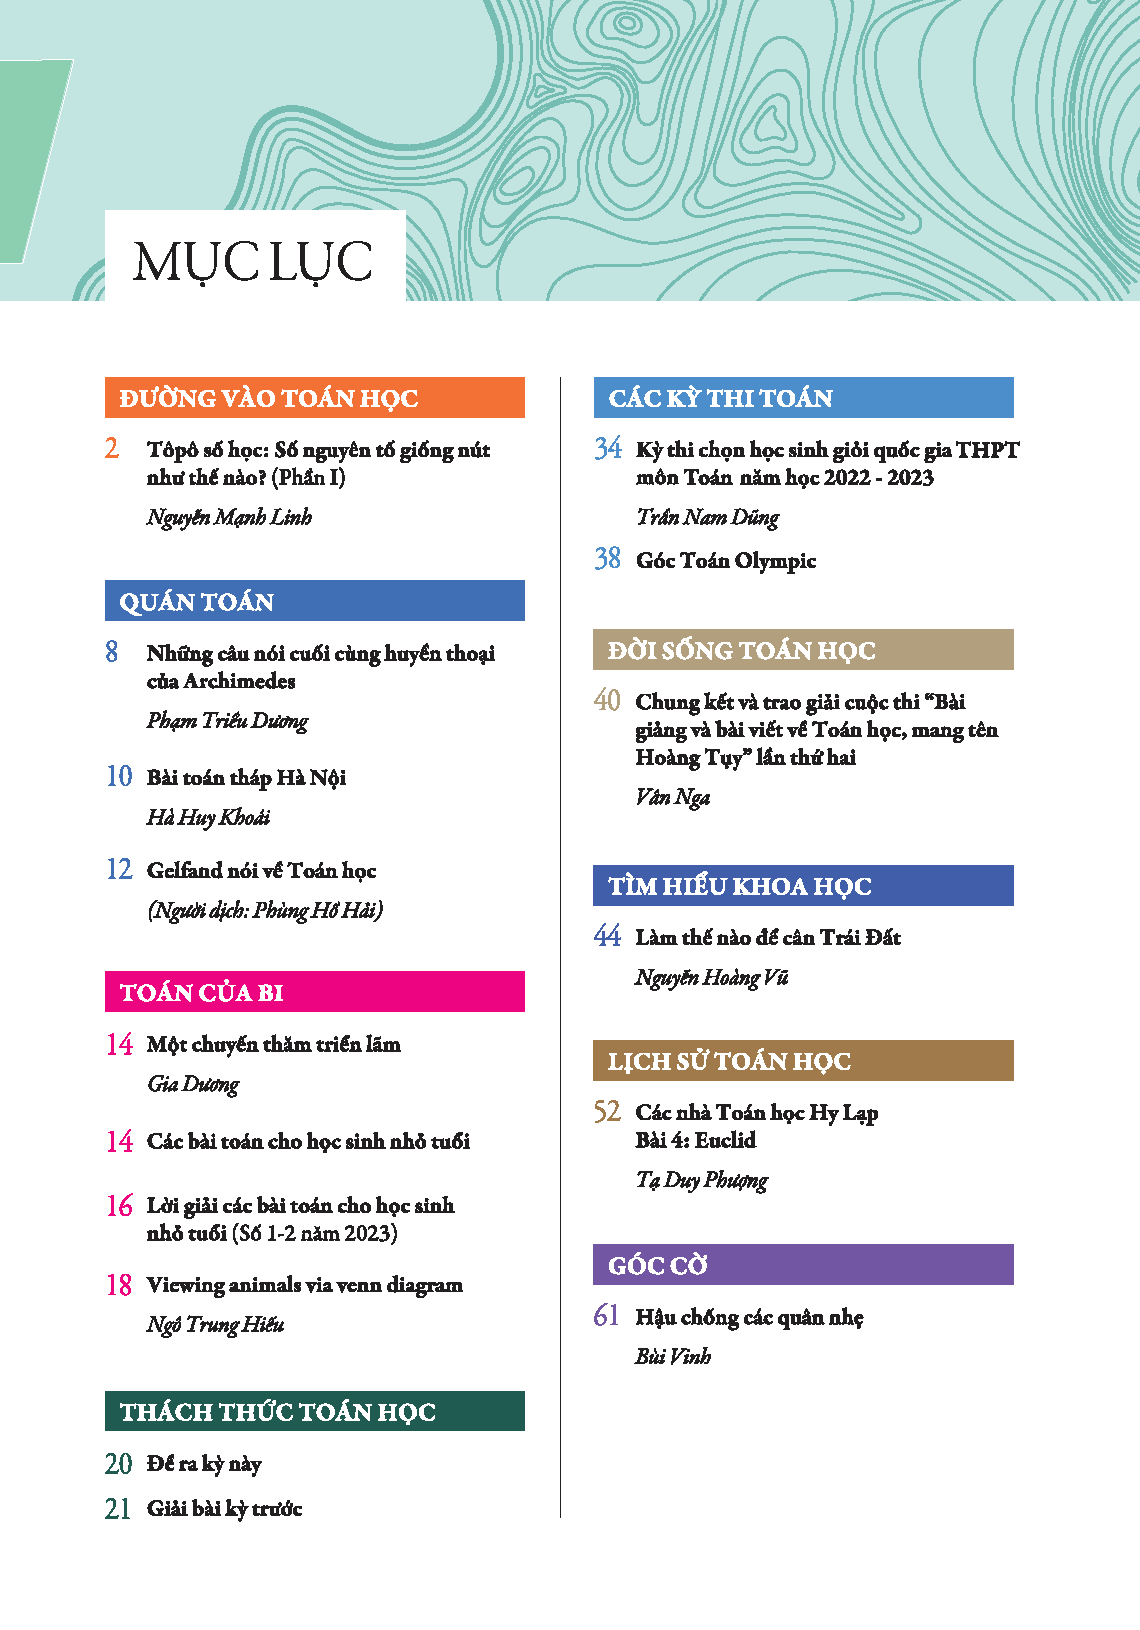
\includegraphics[scale=1]{ML.pdf}}}
%	 \centering
%	 \vspace*{0cm}
%	 \endgroup
%	 \newpage	  
%	 \pagestyle{empty}

%	\setcounter{page}{2}
%	\setcounter{figure}{0}
%	\thispagestyle{duongvaotoanhocnone}
\pagestyle{duongvaotoanhoc}
\everymath{\color{duongvaotoanhoc}}
\graphicspath{{../duongvaotoanhoc/pic/}}
\blfootnote{$^1$\color{duongvaotoanhoc}Universit\'e Paris--Saclay.}
\begingroup
\AddToShipoutPicture*{\put(0,616){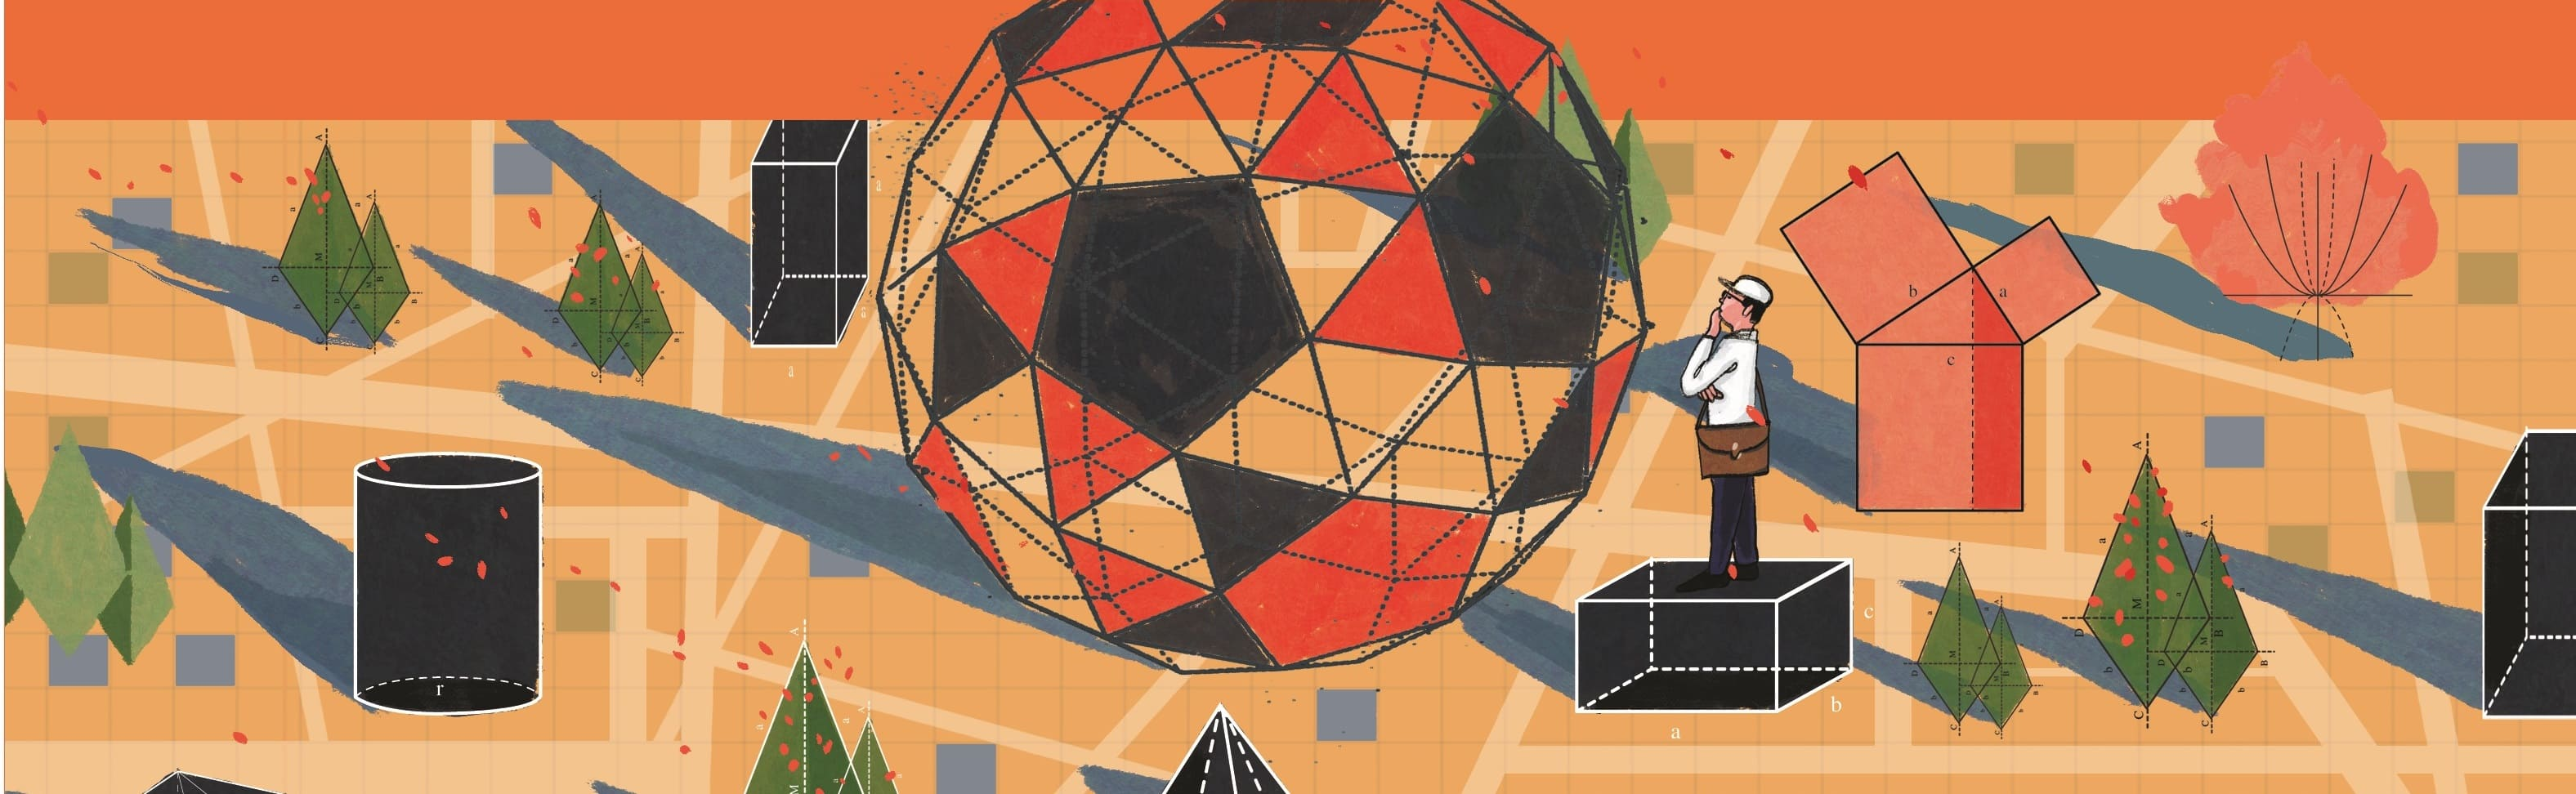
\includegraphics[width=19.3cm]{../bannerduongvao}}}
\AddToShipoutPicture*{\put(58,525){
\includegraphics[scale=1]{../tieude.pdf}}}
\centering
\endgroup
\vspace*{180pt}

\begin{multicols}{2}	
	\textbf{\color{duongvaotoanhoc}Lược đồ}
	\vskip 0.1cm
	Bây giờ, hãy dạo qua thế giới hình học đại số một chút. Với ý tưởng tiên phong của Descartes là nghiên cứu các đối tượng hình học bằng các hệ tọa độ và phương trình đa thức, người ta đã dần dần phát triển hình học đại số. Khác với những người bạn bên tôpô học, các nhà hình học đại số nghiên cứu các đối tượng cứng nhắc hơn: tập nghiệm của các hệ phương trình đa thức. Sau một thời gian, giới toán học nhận ra rằng các trực giác hình học thường mang đến các chứng minh không chặt chẽ và đặc biệt là không giúp gì được ở số chiều cao hơn. Họ đã chuyển sang dùng đại số giao hoán làm công cụ chính để nghiên cứu hình học. Grothendieck, nhà toán học được công nhận rộng rãi là có ảnh hưởng nhất thế kỷ XX, đã cách mạng hóa hình học đại số một lần nữa bằng định nghĩa {\bf\color{duongvaotoanhoc} lược đồ}.
	\vskip 0.1cm
	Ta quay lại với khái niệm trường. Nếu bỏ qua việc luôn làm được phép chia, ta thu được khái niệm {\bf\color{duongvaotoanhoc} vành}. Chẳng hạn, $\mathbb{Z}$ và $\mathbb{Z}/n\mathbb{Z}$ là các vành (phép cộng và phép nhân được hiểu theo nghĩa hiển nhiên). Chú ý rằng ta vẫn yêu cầu làm được phép trừ, nên $\mathbb{N}$ không phải là một vành. Với mỗi vành $R$, ta xây dựng được một không gian tôpô $\text{Spec}(R)$, được gọi là {\bf\color{duongvaotoanhoc} phổ} của $R$. Nếu chỉ nhìn $\text{Spec}(R)$ như một không gian thì ta mất rất nhiều thông tin. Chẳng hạn, phổ của một trường luôn là một điểm. Vì thế, người ta đã làm giàu $\text{Spec}(R)$ một cấu trúc gọi là {\bf\color{duongvaotoanhoc} bó}, chúng làm cho $\text{Spec}(R)$ trở thành một lược đồ.
	\vskip 0.1cm
	Cũng như việc người ta quan tâm đến các hàm liên tục giữa các không gian tôpô, trong hình học đại số người ta quan tâm đến các {\bf\color{duongvaotoanhoc} cấu xạ} giữa các lược đồ. Một cấu xạ $\text{Spec}(R) \to \text{Spec}(S)$ đơn giản được cho bởi một {\bf\color{duongvaotoanhoc} đồng cấu vành} theo chiều ngược lại $f: S \to R$, đồng cấu ở đây nghĩa là $f(x+y) = f(x)+f(y)$, $f(xy) = f(x)f(y)$ và $f(1) = 1$. Chẳng hạn, $\mathbb{Z}$ là một vành con của $\mathbb{Q}$, và phép bao hàm $\mathbb{Z} \to \mathbb{Q}$ cho ta một cấu xạ $\text{Spec}(\mathbb{Q}) \to \text{Spec}(\mathbb{Z})$. Về mặt tôpô thì $\text{Spec}(\mathbb{Q})$ chỉ có một điểm, nên ảnh của cấu xạ này là một điểm của $\text{Spec}(\mathbb{Z})$, được gọi là {\bf\color{duongvaotoanhoc} điểm tổng quát}. Với mỗi số nguyên tố $p$, phép lấy dư modulo $p: \mathbb{Z} \to \mathbb{F}_p$ cho ta một cấu xạ $\text{Spec}(\mathbb{F}_p) \to \text{Spec}(\mathbb{Z})$, đó là một {\bf\color{duongvaotoanhoc} điểm đóng}. Các điểm đóng này và điểm tổng quát tạo nên không gian $\text{Spec}(\mathbb{Z})$. Khác với các không gian Euclid, tôpô trên lược đồ $\text{Spec}(\mathbb{Z})$ rất thô: điểm tổng quát là một điểm nhưng lại trù mật trong cả không gian (người ta hay nói ``điểm tổng quát là điểm nằm ở mọi nơi, nhưng không nằm cụ thể ở đâu cả'').
	\vskip 0.1cm
	Quay lại với lý thuyết không gian phủ. Khi áp dụng nó cho lược đồ, ta không thể chỉ xét khía cạnh tôpô ngây thơ được. Ta muốn $\text{Spec}(\mathbb{F}_p)$ giống với đường tròn $\mathbb{S}^1$, nhưng $\text{Spec}(\mathbb{F}_p)$ lại chỉ có một điểm. Vấn đề với không gian tôpô $\text{Spec}(R)$ là nó có quá ít lân cận, mỗi lân cận đều quá lớn. Cách khắc phục là sáng tạo ra một khái niệm tôpô mới dùng được cho các lược đồ (thứ mà ngày nay gọi là tôpô Grothendieck), với các ``lân cận'' mới. Một trong những loại tôpô đủ mạnh để phân biệt các ``không gian 1 điểm'' $\text{Spec}(K)$ (với $K$ là các trường) là {\bf\color{duongvaotoanhoc} tôpô étale}. Từ ``étale'' được lấy từ văn học Pháp, mang nghĩa nôm na là trạng thái dịu dàng của biển. Với công cụ mới này, người ta định nghĩa được khái niệm nhóm cơ bản étale của lược đồ. Chẳng hạn, nhóm cơ bản étale của $\text{Spec}(\mathbb{F}_p)$ là một nhóm có cùng họ hàng với $\mathbb{Z}$, gọi là ``$\mathbb{Z}$ mũ''. Điều này giải thích vì sao việc coi $\text{Spec}(\mathbb{F}_p)$ như đường tròn $\mathbb{S}^1$ là hợp lý. Tương tự, khái niệm phủ trong thế giới lược đồ phải được hiểu là phủ étale. Đối với các trường, một phủ étale của $\text{Spec}(K)$ đơn giản là $\text{Spec}(L)$, với $L/K$ là một mở rộng bậc hữu hạn. Như vậy, dù $\text{Spec}(K)$ về mặt tôpô chỉ một $1$ điểm, nó lại có nhóm cơ bản étale không tầm thường, hay có rất nhiều phủ. 
	\vskip 0.1cm
	Thực ra khái niệm mở rộng trường và mở rộng vành còn cho ta thêm một chút bên phía tôpô, nó ứng với khái niệm {\bf\color{duongvaotoanhoc} phủ phân nhánh}. Nói nôm na, một phủ phân nhánh bậc $n$ là một hàm liên tục $p: Y \to X$ sao cho nếu bỏ đi một số hữu hạn điểm của $X$ (và các điểm của $Y$ nằm trên chúng) thì ta thu được một phủ $n$-tờ. Các điểm bỏ đi kia (cùng các điểm nằm trên) gọi là các {\bf\color{duongvaotoanhoc} điểm rẽ nhánh} của $p$. Hiện tượng rẽ nhánh là phiên bản hình học của hiện tượng ``nghiệm bội'' trong đại số. Ta xét ví dụ khi $Y$ là đường cong elliptic cho bởi phương trình $y^2=x(x-1)(x-2)$ trong $\mathbb{C}^2$ và $X = \mathbb{C}$. Lấy $p$ là phép chiếu lên trục hoành, $p(x,y) = x$. Khi bỏ đi các điểm $0, 1, 2$ khỏi $X$ (và các điểm $(0,0), (1,0), (2,0)$ khỏi $Y$), ta thu được một phủ $2$--tờ: với mỗi $x \neq 0,1,2$ thì phương trình $y^2=x(x-1)(x-2)$ có hai nghiệm phức phân biệt. Ở các điểm $0, 1, 2$ xảy ra hiện tượng rẽ nhánh, phương trình $y^2=0$ có nghiệm kép $y=0$. Ta nói rằng {\bf\color{duongvaotoanhoc} chỉ số rẽ nhánh} của $p$ tại các điểm $(0,0)$, $(1,0)$, $(2,0)$ bằng $2$.
	\vskip 0.1cm
	\textbf{\color{duongvaotoanhoc}Lý thuyết số đại số}
	\vskip 0.1cm
	Để tìm hiểu các phủ (étale) phân nhánh của lược đồ $\text{Spec}(\mathbb{Z})$, ta bắt đầu từ điểm tổng quát: Phủ étale của $\text{Spec}(\mathbb{Q})$ thì có dạng $\text{Spec}(K)$, với $K = \mathbb{Q}(\alpha)$, và $\alpha$ là nghiệm của một đa thức bậc $n$ bất khả quy với hệ số hữu tỷ. Số $\alpha$ như vậy được gọi là một {\bf\color{duongvaotoanhoc} số đại số}, chẳng hạn $\sqrt{2}, \sqrt[3]{2}, \frac{1 + \sqrt{-3}}{2}$ là các số đại số. Trường $K$ được gọi là một {\bf\color{duongvaotoanhoc} trường số}, và mọi phần tử của nó đều là số đại số. Ta muốn thứ gì đó trong $K$ đóng vai trò như các số nguyên đối với số hữu tỷ. Đó là các {\bf\color{duongvaotoanhoc} số nguyên đại số}. Chúng là những phần tử của $K$ mà là nghiệm của một đa thức với hệ số nguyên và hệ số đầu bằng $1$. Chẳng hạn $\sqrt{2}$ là một số đại số vì nó là nghiệm của $x^2 - 2$. $\frac{1 + \sqrt{5}}{2}$ cũng là một số nguyên đại số (dù trông không có vẻ vậy) vì nó là nghiệm của $x^2-x-1$. Các số nguyên đại số trong $K$ tạo thành một vành $\mathcal{O}$. Việc chuyển từ $\mathbb{Z}$ sang $\mathcal{O}$ là chuyển từ lý thuyết số sơ cấp sang lý thuyết số đại số. Một bài tập đơn giản (bằng cách dùng phân tích duy nhất ra thừa số nguyên tố) là: Các số nguyên đại số trong $\mathbb{Q}$ chính là các số nguyên theo nghĩa cổ điển.
	\vskip 0.1cm
	Lý thuyết số đại số xuất phát từ nỗ lực chứng minh định lý lớn Fermat của Cauchy, Lamé... Ý tưởng như sau: với phương trình $x^2 + y^2 = z^2$ chẳng hạn, ta giải bằng cách đưa về $x^2=z^2-y^2=(z-y)(z+y)$, sau đó lập luận (với phân tích duy nhất ra thừa số nguyên tố) rằng $z-y$ và $z+y$ phải là các số chính phương. Bây giờ, xét phương trình $x^p+y^p=z^p$, với p là số nguyên tố lẻ (dễ thấy ta chỉ cần xét trường hợp này). Để phân tích triệt để $z^p-y^p$ thành các nhân tử bậc nhất, ta buộc phải dùng căn bậc $p$ phức của $1$. Gọi nó là $\zeta = \cos(\frac{2\pi}{p})+i \cdot \sin(\frac{2\pi}{p})$. Thế thì $\zeta$ là một số nguyên đại số (nghiệm của phương trình $x^p - 1$). Và như vậy ta đưa về chứng minh rằng phương trình trên không có nghiệm trong vành mới $\mathbb{Z}[\zeta]$, vành các số nguyên đại số của $\mathbb{Q}(\zeta)$. Sơ hở của cách tiếp cận này là lập luận như trong trường hợp $p=2$ không còn đúng nữa, vì nói chung không có phân tích duy nhất ra thừa số nguyên tố trong $\mathbb{Z}[\zeta]$.
	\vskip 0.1cm
	Một ví dụ về sự không tồn tại của phân tích duy nhất là trường số $K = \mathbb{Q}(\sqrt{-5})$. Vành số nguyên đại số của nó là $\mathcal{O} = \mathbb{Z}[\sqrt{-5}]$, gồm các số có dạng $a+b\sqrt{-5}$ với $a,b \in \mathbb{Z}$. Số $6$ có thể phân tích thành $6 = 2 \cdot 3 = (1+\sqrt{-5}) \cdot (-\sqrt{-5})$. Để thấy rằng hai phân tích này là triệt để và thực sự khác nhau, ta định nghĩa {\bf\color{duongvaotoanhoc} chuẩn} của một số $a+b\sqrt{-5}$ bởi $N(a+b\sqrt{-5}) = a^2 + 5b^2$. Đây là một số tự nhiên, và ta thấy ngay rằng $N(xy) = N(x)N(y)$. Trong phân tích $6 = 2 \cdot 3 = (1+\sqrt{-5}) \cdot (-\sqrt{-5})$, ta có $N(2) = 4, N(3) = 9, N(1+\sqrt{-5}) = N(1-\sqrt{-5}) = 6$, nên các nhân tử xuất hiện ở hai phân tích thực sự khác nhau.  Ngoài ra, về cơ bản ta không thể phân tích thêm được nữa, vì không có phần tử nào có chuẩn bằng $2$ hoặc $3$ (một tính toán số học đơn giản cho thấy rằng phương trình các $a^2 + 5b^2 = 2$ và $a^2 + 5b^2 = 3$ đều không có nghiệm nguyên). Điều này cho thấy sự thiếu sót của phân tích duy nhất ra thừa số nguyên tố trong $\mathbb{Z}[\sqrt{-5}]$.
	\vskip 0.1cm
	Sự sụp đổ của phân tích duy nhất trong $\mathcal{O}$ đã chấm dứt hi vọng chứng minh định lý lớn Fermat bằng lý thuyết số đại số cổ điển. Dù vậy, vành $\mathcal{O}$ vẫn giữ được một tính chất của vành $\mathbb{Z}$; nó là một {\bf\color{duongvaotoanhoc} vành Dedekind}. Thay vì phân tích duy nhất của các số, người ta định nghĩa khái niệm {\bf\color{duongvaotoanhoc} số lý tưởng} (cái mà ngày nay gọi là {\bf\color{duongvaotoanhoc} iđêan}). Đại khái nó là thứ gì đó cho phép nói về quan hệ chia hết cũng như làm phép nhân. Việc $\mathcal{O}$ là vành Dedekind có nghĩa là mọi số lý tưởng đều phân tích một cách duy nhất ra các số lý tưởng nguyên tố. Một số nguyên đại số $a \in \mathcal{O}$ định nghĩa một số lý tưởng $(a)$, được gọi là một số lý tưởng chính. Hai số $a$ và $b$ định nghĩa cùng một số lý tưởng nếu chúng {\bf\color{duongvaotoanhoc} liên kết}, nghĩa là $a|b$ đồng thời $b|a$. Nói riêng, nếu là $u|1$ thì $(u) = (1)$. Nếu tất cả số lý tưởng nguyên tố đều có dạng trên thì $\mathcal{O}$ có phân tích duy nhất của các số (thực sự). Điều này không đúng trong $\mathbb{Z}[\sqrt{-5}]$; cụ thể là khi phân tích $(6) = (2) \cdot (3) = (1 + \sqrt{-5}) \cdot (1 - \sqrt{-5})$, ta vẫn phân tích được tiếp: $(2) = \mathfrak{p}_1\mathfrak{p}_2$, $(3) = \mathfrak{p}_3\mathfrak{p}_4$, $(1 + \sqrt{-5}) = \mathfrak{p}_1\mathfrak{p}_3$, $(1 - \sqrt{-5}) = \mathfrak{p}_2\mathfrak{p}_4$, trong đó $\mathfrak{p}_1, \mathfrak{p}_2, \mathfrak{p}_3, \mathfrak{p}_4$ là các số lý tưởng nguyên tố {\it không chính}. Chuẩn của chúng lần lượt là $N(\mathfrak{p}_1) = N(\mathfrak{p}_2) = 2$ và $N(\mathfrak{p}_3) = N(\mathfrak{p}_4) = 3$. Như vậy ta có phân tích duy nhất của $(6)$ thành các số lý tưởng.
	\vskip 0.1cm
	Cũng như mỗi số nguyên tố $p$ ứng với các điểm đóng $\text{Spec}(\mathbb{F}_p) \to \text{Spec}(\mathbb{Z})$, mỗi số lý tưởng nguyên tố $\mathfrak{p}$ trong trong $\mathcal{O}$ cho ta một trường hữu hạn $\mathbb{F}_{\mathfrak{p}}$ (gọi là {\bf\color{duongvaotoanhoc} trường thặng dư} của $\mathfrak{p}$), cùng một điểm đóng $\text{Spec}(\mathbb{F}_{\mathfrak{p}}) \to \text{Spec}(\mathcal{O})$. Cùng với điểm tổng quát $\text{Spec}(K)$, chúng tạo thành lược đồ $\text{Spec}(\mathcal{O})$. Vì $\mathbb{Z}$ là một vành con của $\mathcal{O}$, ta có một cấu xạ $\text{Spec}(\mathcal{O}) \to \text{Spec}(\mathbb{Z})$, một phủ étale phân nhánh. Mỗi số nguyên tố $p$ trong $\mathbb{Z}$ có thể không còn là số lý tưởng nguyên tố trong $\mathcal{O}$, nó phân rã thành tích của một số hữu hạn số lý tưởng nguyên tố, $(p) = \mathfrak{p_1}\mathfrak{p_2}\cdots\mathfrak{p_n}$. Các số lý tưởng nguyên tố xuất hiện trong phân tích trên chính xác là những điểm của $\text{Spec}(\mathcal{O})$ nằm trên điểm đóng của $\text{Spec}(\mathbb{Z})$ ứng với $p$. Hiện tượng phân nhánh nhánh xảy ra nếu có một số lý tưởng $\mathfrak{p}_i$ xuất hiện nhiều lần trong phân tích trên, ta gọi đó số lần đó là {\bf\color{duongvaotoanhoc} chỉ số rẽ nhánh} của $\mathfrak{p}_i$, nó đóng vai trò như chỉ số rẽ nhánh trong tôpô cổ điển.
	\vskip 0.1cm
	Một bất đẳng thức trong lý thuyết số đại số, {\it chặn Minkowski}, cho phép xác định cụ thể phân tích trên. Hơn thế nữa, nó còn cho ta biết chính xác khi nào thì một số nguyên tố $p$ rẽ nhánh trong $\mathcal{O}$. Một hệ quả của nó là với mọi trường số $K$, luôn có ít nhất một số nguyên tố $p$ rẽ nhánh trong vành $\mathcal{O}$ các số nguyên đại số trong $K$, nghĩa là $\text{Spec}(\mathbb{Z})$ không có phủ  étale không rẽ nhánh nào ngoài phủ tầm thường (cho bởi ánh xạ đồng nhất $\mathbb{Z} \to \mathbb{Z}$), hay nó là đơn liên.
	\vskip 0.1cm
	\textbf{\color{duongvaotoanhoc}Nút}
	\vskip 0.1cm
	Trong thế giới của các không gian tôpô thì có rất nhiều không gian đơn liên, và ta muốn tìm cái nào giống với $\text{Spec}(\mathbb{Z})$. Sự đột phá nằm ở các phát hiện sau đây của Mumford, Manin, và sau này là Mazur. Ở phía tôpô, các khái niệm điểm ($0$--chiều), đường ($1$--chiều), mặt ($2$--chiều) được tổng quát lên thành các đa tạp. Một đa tạp $3$--chiều là một không gian tôpô mà nhìn địa phương thì giống như không gian Euclid $\mathbb{R}^3$ (cũng như bề mặt trái đất là một đa tạp $2$--chiều, nhìn địa phương thì giống như mặt phẳng).
	\vskip 0.1cm
	Bên cạnh nhóm cơ bản, tôpô đại số cổ điển còn cung cấp các bất biến đại số khác cho các không gian tôpô, gọi là các {\bf\color{duongvaotoanhoc} nhóm đồng điều}. Nhóm đồng điều bậc $n$ của một đa tạp $X$ được xây dựng như sau: Xét các tổ hợp tạo thành từ một số đa tạp con $n$--chiều (chúng được gọi là các {\bf\color{duongvaotoanhoc} $n$-dây chuyền}). Nếu chúng tạo thành một vòng kín, ta gọi nó là một {\bf\color{duongvaotoanhoc} $n$--chu trình}. Nếu nó tạo thành biên của một đa tạp con $(n+1)$--chiều, ta gọi nó là một {\bf\color{duongvaotoanhoc} $n$--biên}. Một $n$--biên thì luôn là một $n$--chu trình. Nhóm $H_n(X)$ được định nghĩa là chênh lệch giữa các nhóm các $n$--chu trình và nhóm các $n$--biên: một $n$--chu trình mà không phải $n$--biên thì nó bao quanh một ``lỗ thủng'' $(n+1)$--chiều; như vậy các nhóm đồng điều phát hiện các lỗ thủng trên $X$. Phiên bản đối ngẫu của đồng điều là {\bf\color{duongvaotoanhoc} đối đồng điều}, các nhóm $H^n(X)$. Về cơ bản thì chúng cũng phát hiện các lỗ thủng. Về mặt kỹ thuật thì chúng dễ tính toán hơn đồng điều một chút, đồng thời có nhiều cấu trúc hơn. {\it Đối ngẫu Poincaré} nói rằng nếu $X$ là một đa tạp đóng, khả định hướng, $d$--chiều, thì ta có một đối ngẫu hoàn hảo giữa hai nhóm $H^{d-i}(X)$ và $H^i(X)$ với mỗi $i = 0,1,\ldots,d$.
	\vskip 0.1cm
	Với các lược đồ, các nhóm đối đồng điều nhìn chung không cho thông tin gì (phần lớn chúng bằng $0$) khi ta tính theo tôpô thông thường. Một lần nữa nhờ công của Grothendieck, ta có thể tính {\bf\color{duongvaotoanhoc}đối đồng điều étale}.  Trên một trường, chúng được gọi là {\bf\color{duongvaotoanhoc}đối đồng điều Galois}, một công cụ đã được dùng từ lâu trước đó trong số học. Với các trường hữu hạn, đối đồng điều Galois của chúng rất đơn giản, chúng khác $0$ ngoài bậc $0$ và $1$, và ta có một đối ngẫu hoàn hảo giữa các nhóm đối đồng điều ở hai bậc này. Điều này tương tự với đối ngẫu Poincaré cho các đa tạp $1$--chiều, khẳng định thêm niềm tin rằng phổ của trường hữu hạn là phiên bản đại số của đường tròn. 
	\vskip 0.1cm
	Đối với các lược đồ $\text{Spec}(\mathcal{O})$, với $\mathcal{O}$ là vành số nguyên đại số của một trường số $K$ nào đó, các nhóm đối đồng điều étale thỏa mãn đối ngẫu giữa bậc $0$ và bậc $3$ cũng như bậc $1$ và bậc $2$. Các kết quả này được gọi là {\it đối ngẫu Artin--Verdier}, được khám phá khi áp dụng đối đồng điều étale cho lý thuyết trường các lớp toàn cục, một phần của lý thuyết số. Điều này gợi cho ta rằng phiên bản tôpô của $\text{Spec}(\mathcal{O})$ ``nên" là các đa tạp $3$--chiều. Vậy $\text{Spec}(\mathbb{Z})$ ứng với đa đạp đóng $3$--chiều nào? Ta thấy ở trên rằng $\text{Spec}(\mathbb{Z})$ đơn liên, và đa tạp đóng $3$--chiều đơn liên thì chỉ có thể đồng phôi với mặt (siêu) cầu  $\mathbb{S}^3$! Đó là nội dung của {\it giả thuyết Poincaré}, bài toán duy nhất đã được giải trong $7$ bài toán thiên niên kỷ. Tác giả của lời giải, thiên tài lập dị Perelman, đã từ chối cả Huy chương Fields lẫn Giải thưởng Thiên niên kỷ (Millennium Prize) cho công trình vô song của mình.
	\vskip 0.1cm
	Sau khi bỏ ra rất nhiều công sức, ta đã thấy được cầu nối mong manh giữa tôpô học và số học, rằng phiên bản số học của $\mathbb{S}^1$ là (phổ của) một trường hữu hạn, và của một đa tạp đóng $3$--chiều là vành các số nguyên đại số của một trường số. Bây giờ là lúc chúng ta thu hoạch kết quả, chiêm ngưỡng những sự tương tự đáng ngạc nhiên dựa trên cầu nối này. Một số lý tưởng nguyên tố $\mathfrak{p}$ trong $\mathcal{O}$ cho ta một phép nhúng $\text{Spec}(\mathbb{F}_\mathfrak{p}) \hookrightarrow \text{Spec}(\mathcal{O})$. Về phía tôpô, ta xét các phép nhúng $\mathbb{S}^1 \hookrightarrow M$, với $M$ là một đa tạp (đóng, khả định hướng) $3$-chiều. Chúng được gọi là các {\bf\color{duongvaotoanhoc} nút} trong $M$. Nói riêng, phiên bản tôpô của mỗi số nguyên tố $p$ (với phép nhúng tương ứng $\text{Spec}(\mathbb{F}_p) \hookrightarrow \text{Spec}(\mathbb{Z})$) là một nút trong $\mathbb{S}^3$ (ta sẽ tập trung vào các nút này). Từ một định lý sâu sắc trong tôpô học, {\it định lý Borsuk--Ulam}, ta có thể chỉ ra rằng một phép nhúng như thế không thể là toàn ánh, nghĩa là ta có thể xem một nút như một phép nhúng từ $\mathbb{S}^1$ vào $\mathbb{S}^3$ bỏ đi một điểm, nói cách khác chính là không gian Euclid $\mathbb{R}^3$.
	\vskip 0.1cm
	Để biểu diễn một nút $K: \mathbb{S}^1 \hookrightarrow \mathbb{R}^3$ ta có thể chiếu nó lên một mặt phẳng sau cho tại mỗi điểm giao nhau chỉ có đúng $2$ đường đi qua. Chúng ứng với một {\bf\color{duongvaotoanhoc} sợi trên} và một {\bf\color{duongvaotoanhoc} sợi dưới}, ta biểu diễn sợi dưới bằng nét đứt tại giao điểm đó.  Đó là một {\bf\color{duongvaotoanhoc} biểu đồ phẳng} của nút.
	\begin{figure}[H]
		\vspace*{-5pt}
		\centering
		\captionsetup{labelformat= empty, justification=centering}
		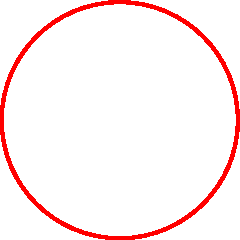
\includegraphics[width= 0.28\linewidth]{unknot.pdf}\quad
		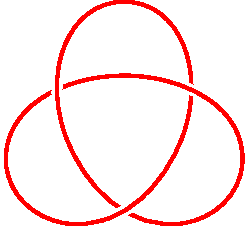
\includegraphics[width= 0.28\linewidth]{trefoil.pdf}\quad
		
\includegraphics[width= 0.28\linewidth]{figure 8.pdf}
		\caption{\small\textit{\color{duongvaotoanhoc}Hình $10$: Biểu đồ phẳng của nút tầm thường, nút ba lá, và nút số $8$.}}
		\vspace*{-10pt}
	\end{figure}
	Tất nhiên, mọi nút đều đồng phôi với $\mathbb{S}^1$. Ta cần cả thông tin về phép nhúng $\mathbb{S}^1 \to \mathbb{R}^3$ để phân biệt các nút với nhau. Các nhà lý thuyết nút gọi sự giống nhau của các nút là {\bf\color{duongvaotoanhoc} đẳng luân}. Một cách trực giác, hai nút đẳng luân nếu ta có thể tháo dỡ một nút rồi buộc thành nút còn lại (mà không cắt được cắt nút ra). Hóa ra, hai nút đẳng luân khi và chỉ khi phần bù của chúng trong $\mathbb{S}^3$ đồng phôi với nhau ({\it định lý Gordon--Luecke}).
	\vskip 0.1cm
	\textbf{\color{duongvaotoanhoc}Từ điển M$^2$KR}
	\vskip 0.1cm
	Từ điển Mazur--Morishita--Kapranov--Reznikov (M$^2$KR) là một danh sách những sự tương tự giữa lý thuyết số và hình học của các đa tạp $3$--chiều; ở đó các số lý tưởng tưởng ứng với các liên kết, các số lý tưởng nguyên tố ứng với các nút. Sau đây là một số tương ứng giữa tôpô và số học trong từ điển này.
	\vskip 0.1cm
	Mỗi số lý tưởng trong $\mathcal{O}$ phân tích thành tích của các số lý tưởng nguyên tố. Phiên bản tôpô của số lý tưởng là {\bf\color{duongvaotoanhoc} liên kết}: một liên kết trong một đa tạp đóng $3$--chiều $M$ là một phép nhúng từ một số hữu hạn bản sao rời rạc của $\mathbb{S}^1$ vào $M$. Các ví dụ về liên kết trong $\mathbb{S}^3$ là {\bf\color{duongvaotoanhoc} liên kết Hopf} và {\bf\color{duongvaotoanhoc} vòng Borromean}, lần lượt được tạo bởi $2$ và $3$ nút tầm thường lồng nhau.
	\begin{figure}[H]
		\vspace*{-15pt}
		\centering
		\captionsetup{labelformat= empty, justification=centering}
		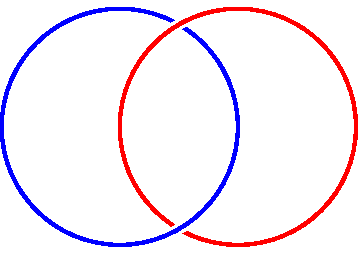
\includegraphics[width= 0.38\linewidth]{hopf.pdf}\quad\quad
		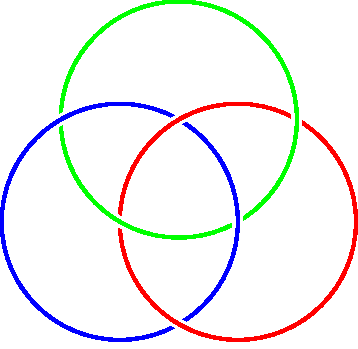
\includegraphics[width= 0.38\linewidth]{borromean.pdf}
		\caption{\small\textit{\color{duongvaotoanhoc}Hình $11$: Biểu đồ phẳng của liên kết Hopf và vòng Borromean.}}
		\vspace*{-10pt}
	\end{figure}
	Để thêm phần thuyết phục rằng tại sao $M$ lại tương ứng với (vành số nguyên đại số) một trường số, ta nhắc đến {\it định lý Alexander}: Mọi đa tạp đóng $3$--chiều đều là một phủ phân nhánh của $\mathbb{S}^3$, trong đó các điểm rẽ nhánh trong $\mathbb{S}^3$ tạo thành một liên kết. Tương tự, một mở rộng $L/K$ của trường số có thể được coi như một phủ phân nhánh giữa hai đa tạp đóng $3$--chiều.
	\vskip 0.1cm
	Một số nguyên đại số $a \in \mathcal{O}$ ứng với một mặt compact $S$ (có thể có biên) nhúng trong đa tạp đóng $3$--chiều $M$. Số lý tưởng chính $(a)$ ứng với biên $\partial S$, đây là một liên kết, và chúng ứng với các $1$--đối biên, tức là phần tử $0$ trong nhóm đồng điều $H_1(M)$. Các số lý tưởng khác tương ứng với các liên kết, chúng là các $1$--chu trình mà không phải biên, đại diện cho các phần tử không tầm thường của $H_1(M)$. Ta biết rằng trong $\mathbb{Z}$ có phân tích duy nhất ra thừa số nguyên tố, hay mọi số lý tưởng nguyên tố đều là số lý tưởng chính. Tương ứng, với $M = \mathbb{S}^3$, ta có $H_1(M) = 0$ (vì $\mathbb{S}^3$ không có lỗ thủng $2$--chiều nào), nghĩa là mọi liên kết đều là biên của một mặt nào đó. Seifert đã đưa ra một thuật toán khá đơn giản để xây dựng một mặt với biên cho trước. Chẳng hạn, {\bf\color{duongvaotoanhoc} mặt Seifert} của liên kết Hopf chính là {\it mặt M\"obius}.
	\begin{figure}[H]
		\vspace*{-5pt}
		\centering
		\captionsetup{labelformat= empty, justification=centering}
		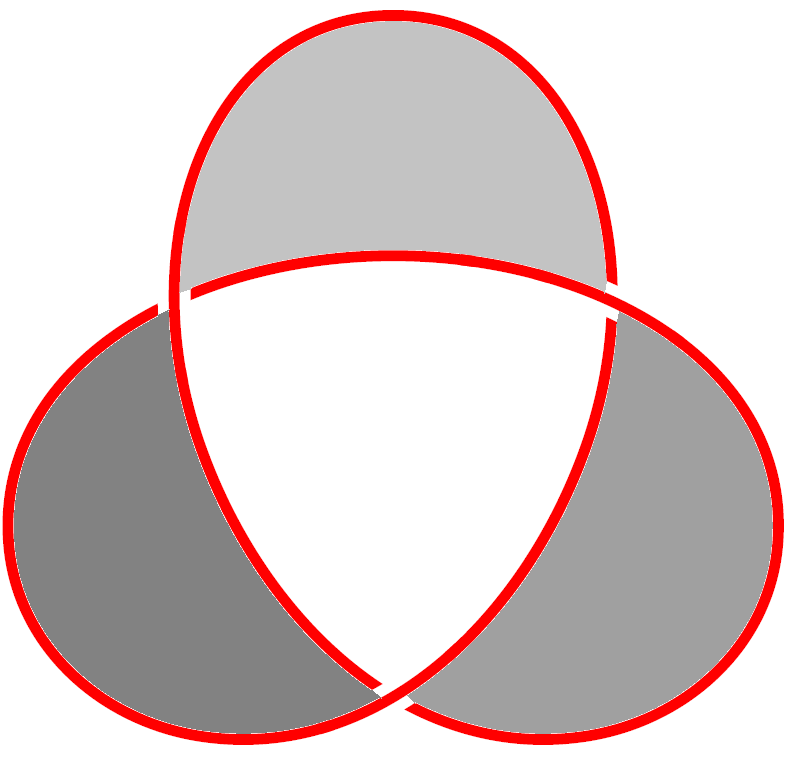
\includegraphics[width= 0.4\linewidth]{seifert1}\quad\quad
		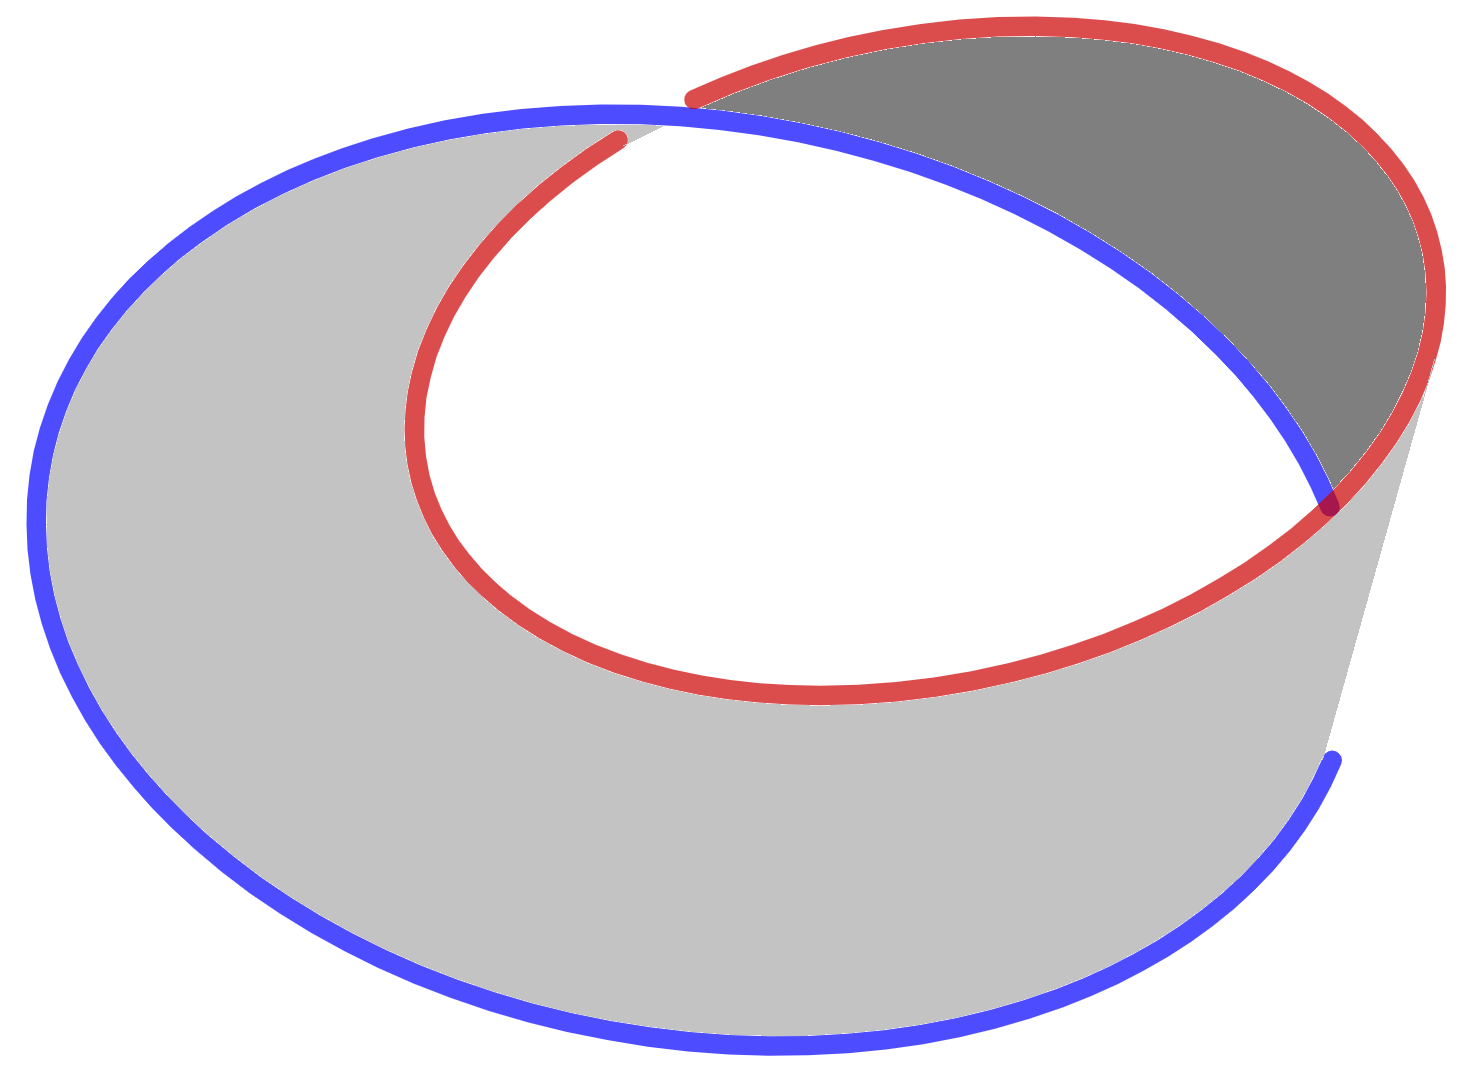
\includegraphics[width= 0.4\linewidth]{seifert2}
		\caption{\small\textit{\color{duongvaotoanhoc}Hình $12$: Mặt Seifert của nút ba lá và của liên kết Hopf (mặt M\"obius).}}
		\vspace*{-10pt}
	\end{figure}
	Sự tương tự tiếp theo: với $p$ là một số nguyên tố, ta xét vành $\mathbb{Z}_p$ các số nguyên $p$--adic cũng như trường $\mathbb{Q}_p$ các số $p$--adic. So với $\text{Spec}(\mathbb{Z})$, phổ $\text{Spec}(\mathbb{Z}_p)$ chỉ còn $2$ điểm là điểm tổng quát $\text{Spec}(\mathbb{Q}_p)$ và điểm đóng $\text{Spec}(\mathbb{F}_p)$, vì thế ta gọi thao tác này {\bf\color{duongvaotoanhoc} địa phương hóa} (tập trung nhìn vào số nguyên tố $p$ và quên đi các số nguyên tố khác). Thao tác này ứng với việc lấy {\bf\color{duongvaotoanhoc} lân cận ống} $V$ của nút, kết quả thu được là một hình xuyến đặc. Dù hình xuyến đặc không đồng phôi với đường tròn, chúng {\bf\color{duongvaotoanhoc} tương đương đồng luân với nhau}, điều này ứng với việc $\text{Spec}(\mathbb{Z}_p)$ và $\text{Spec}(\mathbb{F}_p)$ {\bf\color{duongvaotoanhoc} tương đương đồng luân étale với nhau}. Khi bỏ nút ban đầu khỏi $V$, ta thu được một không gian tương đương đồng luân với mặt xuyến (rỗng). Nhóm cơ bản của mặt xuyến là $\mathbb{Z} \times \mathbb{Z}$, một nhóm được sinh bởi hai phần tử là hai khuyên như trong Hình $13$.
	\begin{figure}[H]
		\vspace*{-5pt}
		\centering
		\captionsetup{labelformat= empty, justification=centering}
		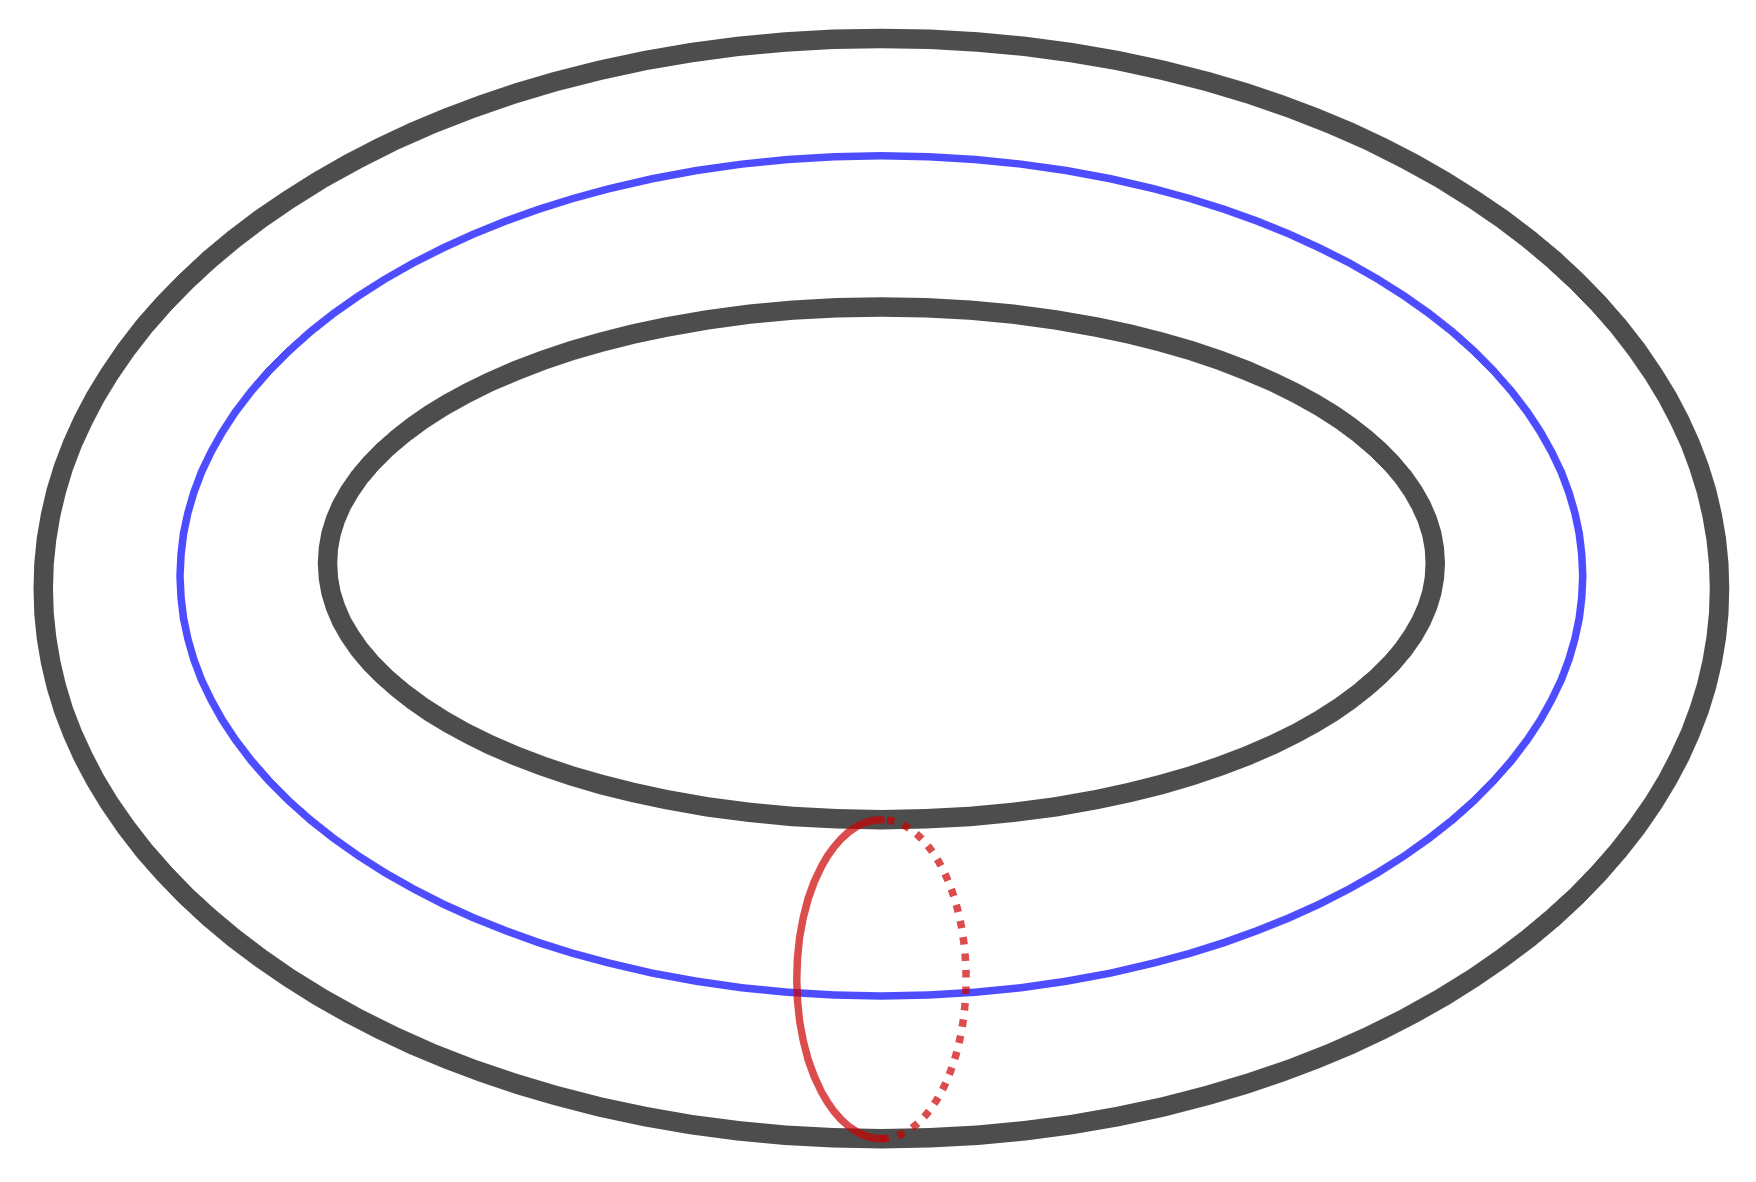
\includegraphics[width= 0.65\linewidth]{h13}
		\caption{\small\textit{\color{duongvaotoanhoc}Hình $13$: Nhóm cơ bản của mặt xuyến được sinh bởi hai khuyên màu xanh và màu đỏ.}}
		\vspace*{-5pt}
	\end{figure}
	Tương ứng, khi bỏ $\text{Spec}(\mathbb{F}_p)$ khỏi $\text{Spec}(\mathbb{Z}_p)$, ta thu được $\text{Spec}(\mathbb{Q}_p)$, và {\bf\color{duongvaotoanhoc} nhóm Galois rẽ nhánh yếu} (một phiên bản nhỏ hơn của nhóm cơ bản étale) của $\mathbb{Q}_p$ cũng được mô tả bởi $2$ phần tử sinh. Sau cùng, lý thuyết trường các lớp địa phương của Tate cho ta các đối ngẫu hoàn hảo giữa đối đồng điều Galois của  $\mathbb{Q}_p$ ở bậc $0$ và bậc $2$, cũng như ở bậc $1$ và chính nó. Tương ứng, ta có đối ngẫu Poincaré cho mặt xuyến, một đa tạp đóng $2$--chiều.
	\vskip 0.1cm
	\textbf{\color{duongvaotoanhoc}Thao tác trên biểu đồ phẳng}
	\vskip 0.1cm
	Quay lại với sự đẳng luân của các nút. Một câu hỏi rất tự nhiên là làm thế nào để chứng minh hai nút không đẳng luân? Đẳng luân vốn là một điều kiện tôpô quá khó sử dụng. Một khó khăn khi sử dụng các biểu đồ phẳng là hai nút đẳng luôn có thể cho hai biểu đồ phẳng trông rất khác nhau. Vậy vấn đề đầu tiên là ta cần tìm cách phân biệt hai nút qua biểu đồ phẳng của chúng (bài toán nhận biết nút). Điều này có thể được thực hiện một cách tổ hợp. Cụ thể, hai biểu đồ phẳng biểu diễn hai nút đẳng luân khi và chỉ khi tồn tại một chuỗi hữu hạn các thao tác thuộc một trong $4$ kiểu, được gọi là các {\bf\color{duongvaotoanhoc} chuyển động Reidemeister}.
	\begin{figure}[H]
		\vspace*{-10pt}
		\centering
		\captionsetup{labelformat= empty, justification=centering}
		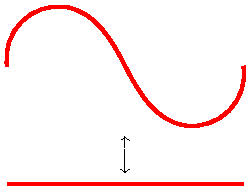
\includegraphics[width= 0.3\linewidth]{R0.pdf}\quad
		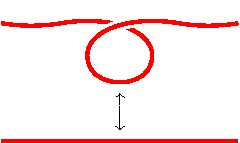
\includegraphics[width= 0.3\linewidth]{R1.pdf}
		\caption{\small\textit{\color{duongvaotoanhoc}R$0$: Phép đẳng luân phẳng.\hspace*{20pt}  RI: Phép xoắn.}}
		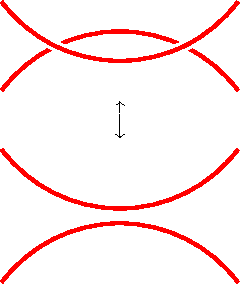
\includegraphics[width= 0.3\linewidth]{R2.pdf}\quad
		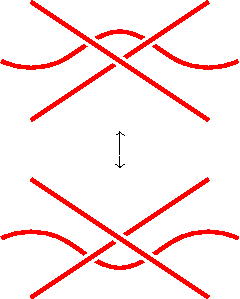
\includegraphics[width= 0.3\linewidth]{R3.pdf}
		\caption{\small\textit{\color{duongvaotoanhoc}RII: Phép đè.\hspace*{30pt} RIII: Phép trượt.}}
		\caption{\small\textit{\color{duongvaotoanhoc}Hình $14$: Các chuyển động Reidemeister.}}
		\vspace*{-10pt}
	\end{figure}
	Từ biểu đồ phẳng của nút, ta dùng các đại lượng không đổi qua các chuyển động Reidemeister, các {\bf\color{duongvaotoanhoc} bất biến nút}. Hai nút có bất biến khác nhau thì phải khác nhau. Một ví dụ như vậy là {\bf\color{duongvaotoanhoc} bất biến tô màu}. Ta nói một biểu đồ phẳng của nút là {\bf\color{duongvaotoanhoc} tô được bằng $\pmb{3}$ màu} nếu mỗi sợi (phần đường cong liên tục giữa hai giao điểm liên tiếp của nút) đều có thể tô được bằng một trong $3$ màu cho trước, sao cho
	\vskip 0.05cm
	$\bullet$ ít nhất hai màu phải được dùng;
	\vskip 0.05cm
	$\bullet$ tại mỗi giao điểm, sợi trên cùng $2$ sợi dưới hoặc là được tô cùng màu, hoặc là được tô $3$ màu khác nhau.
	\vskip 0.05cm
	Ví dụ, nút ba lá hiển nhiên tô được bằng $3$ màu, nút tầm thường hiển nhiên không tô được bằng $3$ màu. Nút số $8$ cũng không tô được bằng $3$ màu. Vậy ít nhất ta biết rằng nút $3$ lá không đẳng luân với nút tầm thường cũng như nút số $8$.
	\vskip 0.05cm
	Hiển nhiên là bất biến tô màu chỉ cho phép phân loại các nút thành $2$ lớp. Ta cần các loại bất biến khác. Ví dụ, xét nút ba lá trái và ảnh gương của nó là nút ba lá phải. Tất nhiên cả hai đều tô được bằng $3$ màu. Rất ngạc nhiên, hai nút này không đẳng luân! Hãy thử dùng các chuyển động Reidemeister để gỡ nút này thành nút kia và bạn sẽ sớm bị thuyết phục. Một bất biến cho phép phân biệt hai nút này là {\bf\color{duongvaotoanhoc} đa thức Alexander}. Đa thức này đến từ {\it lý thuyết Alexander--Fox}, và người ta phát hiện ra phiên bản số học của nó là {\it lý thuyết Iwasawa}. Sự song song của chúng cho phép ta dịch các kết quả từ một bên sang bên còn lại.
	\begin{figure}[H]
		\vspace*{-10pt}
		\centering
		\captionsetup{labelformat= empty, justification=centering}
		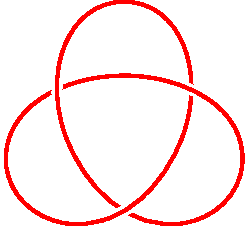
\includegraphics[width= 0.36\linewidth]{trefoil.pdf}\quad\quad
		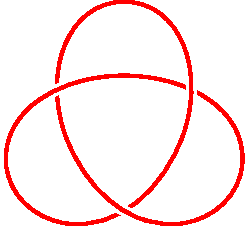
\includegraphics[width= 0.36\linewidth]{mirror trefoil.pdf}
		\caption{\small\textit{\color{duongvaotoanhoc}Hình $15$: Nút ba lá trái và nút ba lá phải.}}
		\vspace*{-10pt}
	\end{figure}
	Một kiểu bất biến khác cho liên kết là {\bf\color{duongvaotoanhoc} số liên kết}. Xét một liên kết được tạo bởi hai nút. Giữa hai nút $L$ và $K$, ta có thể định nghĩa {\bf\color{duongvaotoanhoc} số liên kết} qua biểu đồ phẳng của chúng như sau. Chẳng hạn, tô màu đỏ cho $L$ và màu xanh cho $K$, đồng thời định hướng cho chúng (mỗi nút có thể có $1$ trong $2$ hướng). Tại các điểm trên biểu đồ phẳng mà có một sợi của nút này nằm trên một sợi của nút kia hoặc ngược lại, ta đánh dấu $+$ hoặc $-$ theo quy tắc ở Hình $16$. Sau đó ta lấy số dấu cộng trừ đi số dấu trừ, và lấy kết quả chia đôi. Kết quả cuối cùng thu được được gọi là số liên kết $\text{lk}(L,K)$. Chẳng hạn, số liên kết của hai nút trong liên kết Hopf là $1$ hoặc $-1$, tùy theo cách định hướng hai nút.
	\begin{figure}[H]
		\vspace*{-5pt}
		\centering
		\captionsetup{labelformat= empty, justification=centering}
		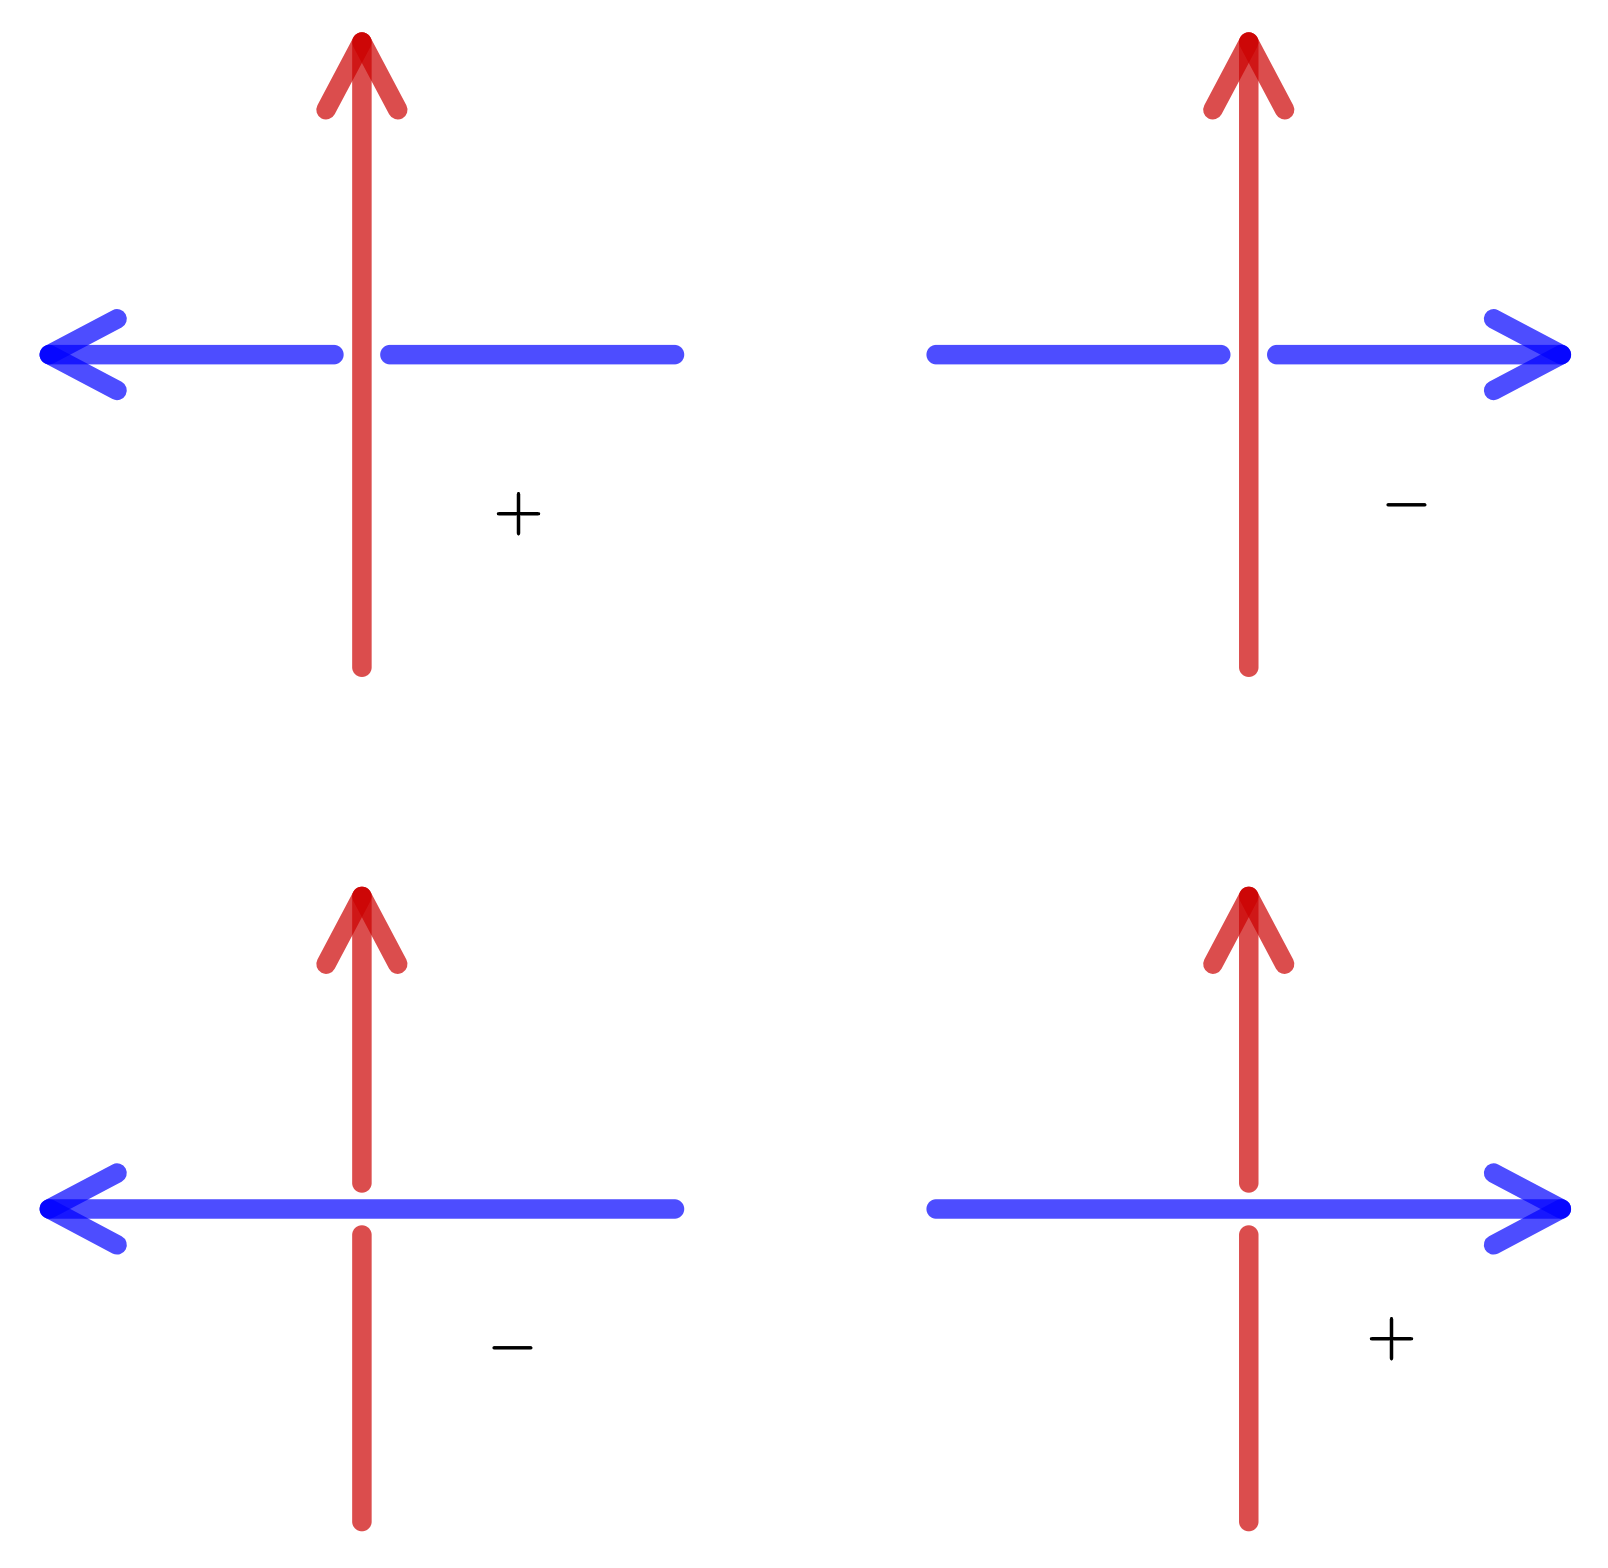
\includegraphics[width= 0.6\linewidth]{h16}
		\caption{\small\textit{\color{duongvaotoanhoc}Hình $16$: Quy tắc tính số liên kết.}}
		\vspace*{-10pt}
	\end{figure}
	Nhiều tính toán cho thấy rằng số liên kết thỏa mãn các tính chất tương tự như {\bf\color{duongvaotoanhoc} ký hiệu Legendre} $\left(\dfrac{p}{q}\right)$ giữa hai số nguyên tố $p, q$ trong lý thuyết thặng dư bậc hai. Ta có thể chứng minh rằng $\text{lk}(K,L) = \text{lk}(L,K)$. Tương ứng, ta có luật tương hỗ bậc hai, nói rằng 
	\begin{align*}
		\left(\dfrac{p}{q}\right) = (-1)^{\tfrac{(p-1)(q-1)}{4}}\left(\dfrac{q}{p}\right).
	\end{align*}
	Bài toán trung tâm của tôpô số học có lẽ là câu hỏi tự nhiên nhất: số nguyên tố nào ứng với nút nào? Đây vẫn là một câu hỏi mở. Nếu một ngày người ta xây dựng được một tương ứng $1-1$ tốt giữa chúng, theo nghĩa mỗi kết quả với số nguyên tố thì ta có kết quả với các nút tương ứng, một số lượng khổng lồ bài toán tôpô học sẽ được giải bằng các kết quả tương tự ở lý thuyết số, và ngược lại.
	
	 Có thể nói, tôpô số học là một trong những ví dụ điển hình nhất về tư tưởng toán học thống nhất, rằng tất cả những đại số, giải tích, hình học, số học... đều chỉ là một.
\end{multicols} 
%	\newpage
%
%	\setcounter{figure}{0}
%	\thispagestyle{quantoannone}
\pagestyle{quantoan}
\everymath{\color{quantoan}}
\graphicspath{{../quantoan/pic/}}
%\blfootnote{\color{quantoan}\color{quantoan}$^*$Nguồn Math. Intellegencer, Số $41$.}
\begingroup
\AddToShipoutPicture*{\put(0,616){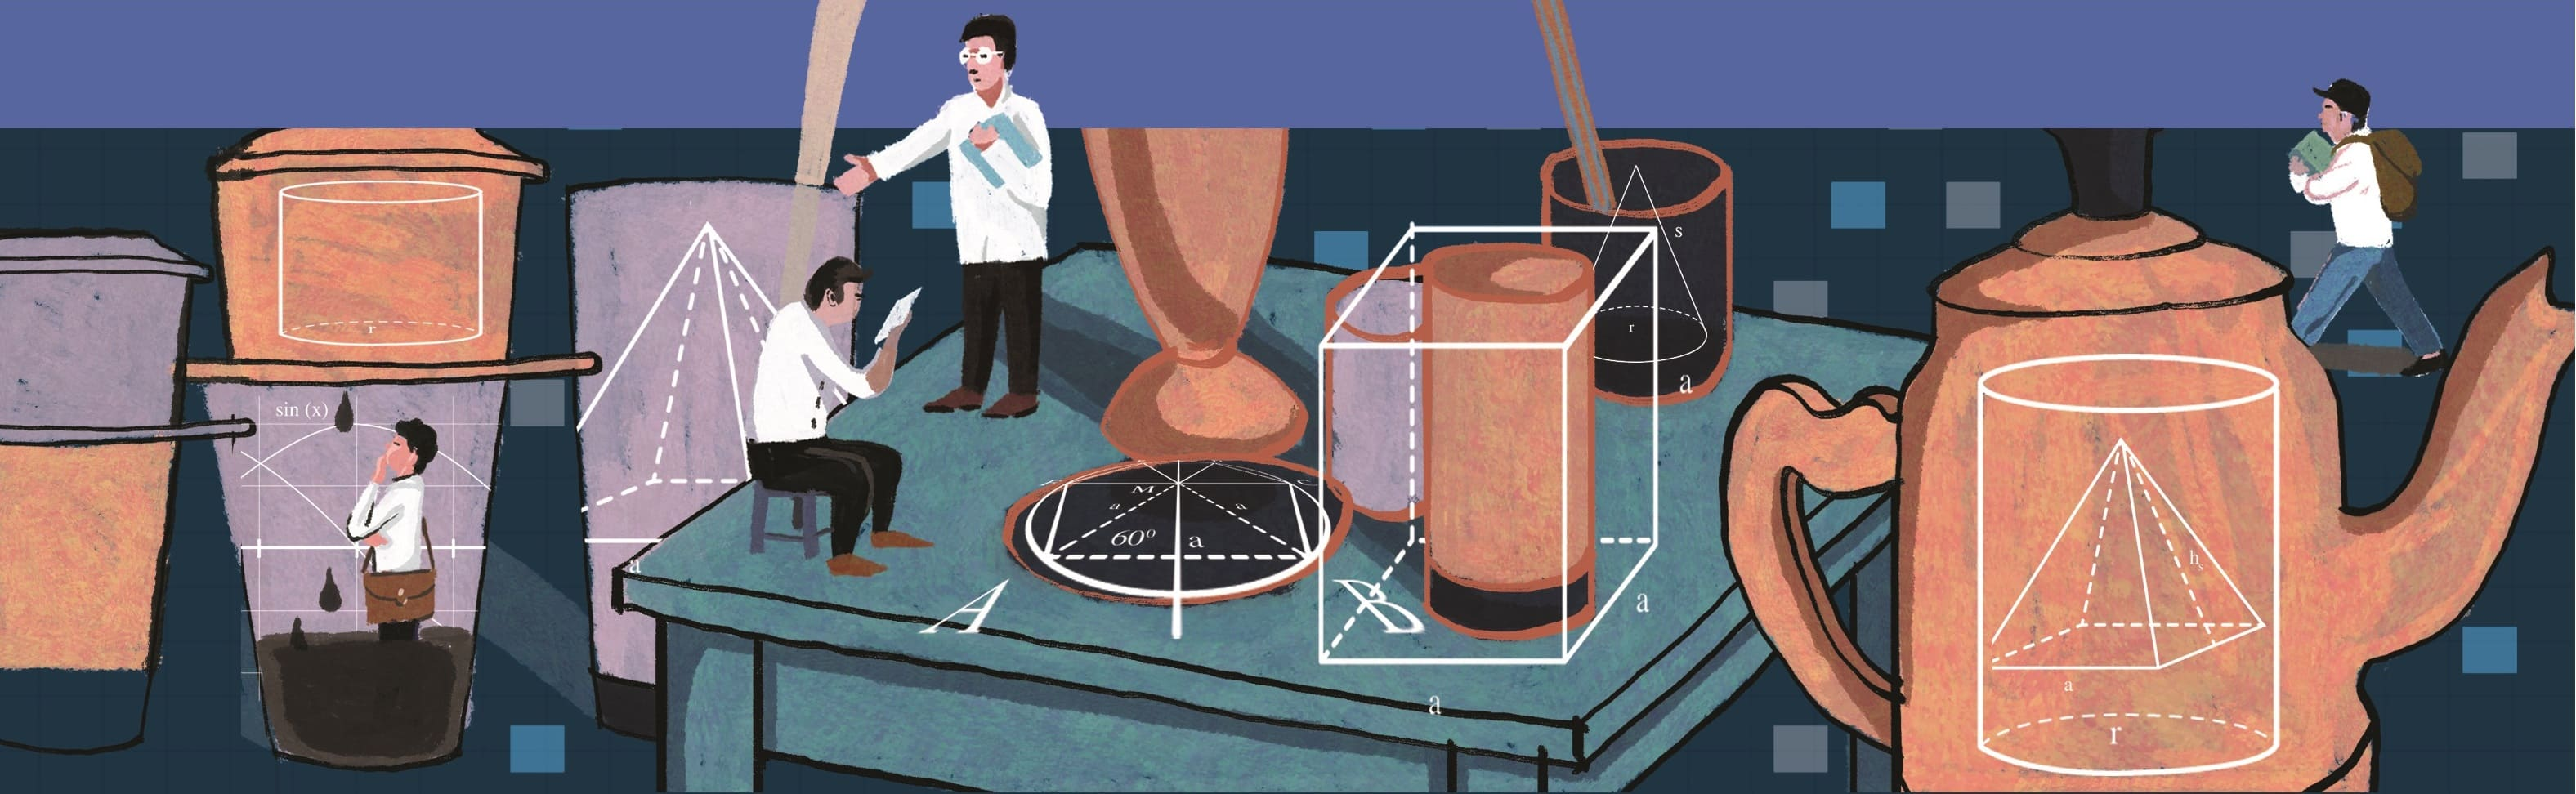
\includegraphics[width=19.3cm]{../bannerquantoan}}}
\AddToShipoutPicture*{\put(120,552){
\includegraphics[scale=1]{../tieude.pdf}}}
\centering
\endgroup
\vspace*{155pt}

\begin{multicols}{2}
	Người ta kể lại rằng nhà toán học Pythagoras đã thiết kế một loại cốc đặc biệt dành cho các học trò của mình (Hình $1$). Ở phần giữa của nó có một lỗ thông xuống đáy được che lại bởi một cấu trúc tạo thành bình thông nhau.
	\begin{figure}[H]
		\vspace*{-5pt}
		\centering
		\captionsetup{labelformat= empty, justification=centering}
		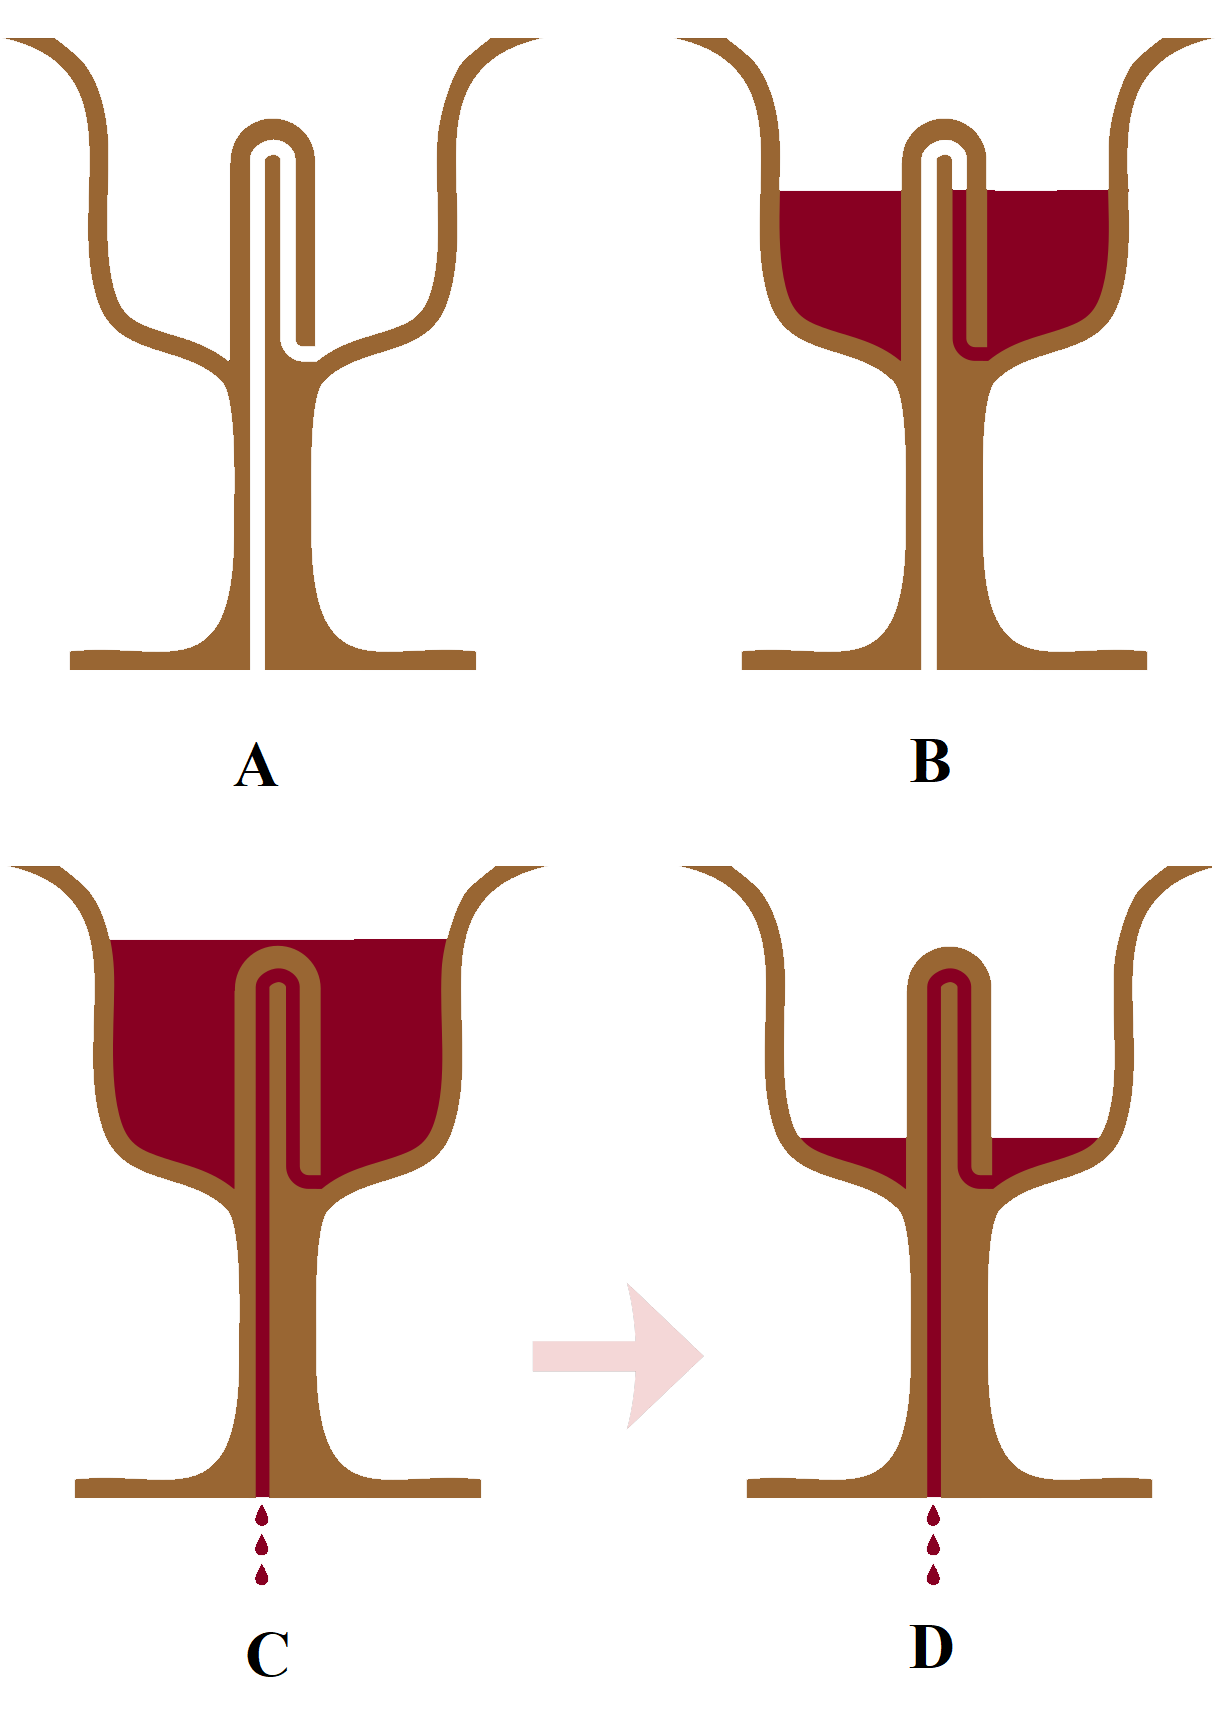
\includegraphics[width= 1\linewidth]{1}
		\caption{\small\textit{\color{quantoan}Hình $1$. Chiếc cốc của Pythagoras. Khi rót đầy chất lỏng vượt ngưỡng, toàn bộ chất lỏng trong cốc sẽ bị chảy ra ngoài}}
		\vspace*{-10pt}
	\end{figure}
	Khi đổ dần rượu vào cốc, mực rượu sẽ dâng lên ở trong cốc cũng như nhánh thông với nó (Hình $1$B). Đến khi mực rượu vượt ngưỡng chứa của nhánh này, nó bắt đầu sẽ bị chảy ra ngoài (Hình $1$C). Nhưng thay vì chỉ rút xuống mức tới hạn trước khi rượu bắt đầu chảy ra, toàn bộ chất lỏng trong cốc lại vẫn tiếp tục tạo thành dòng chảy ra ngoài cho đến khi chảy hết rượu. Những kẻ tham lam sẽ không còn lại gì cả!
	
	Đây là một bài học của Pythagoras cho các học trò của mình về việc phải có chừng mực trong cuộc sống, không được thái quá. Vậy còn bài học về vật lý ở đây là gì? Tại sao rượu lại có thể tiếp tục chảy ngược ra ngoài dù mực rượu trong phần ống cao hơn trong cốc? Những gì ta đã biết về bình thông nhau có bị vi phạm?
	\vskip 0.1cm
	Thực chất của hiện tượng xảy ra trong chiếc cốc của Pythagoras giống với quy trình hoạt động của ống xi phông (Hình $2$). Ống này có dạng ống chữ U ngược với hai đầu đặt ở hai khối chất lỏng khác nhau, một đầu cao hơn đầu còn lại. Chất lỏng trong ống xi phông có thể chảy từ khối chất lỏng cao ngược lên đỉnh chữ U rồi chảy xuống khối chất lỏng ở dưới. Để bắt đầu dòng chảy, người ta cần hút không khí ra khỏi đầu dưới của ống để tạo sự chênh lệch với áp suất khí quyển ở đầu còn lại. Hai mô hình được đưa ra để giải thích hiện tượng này. Trong mô hình thứ nhất, khi chất lỏng chảy vượt qua đỉnh của chữ U ngược, nó tạo ra một vùng áp suất thấp nên áp suất khí quyển từ đầu đường ống sẽ tiếp tục đẩy chất lỏng đi. Mô hình thứ hai dựa trên lực liên kết phân tử, trong đó sự kết dính giữa các khối nước sẽ kéo chúng theo nhau tạo thành dòng chảy. Việc mô hình nào là chính xác vẫn còn là một vấn đề đang được khoa học nghiên cứu.
	\begin{figure}[H]
		\vspace*{-5pt}
		\centering
		\captionsetup{labelformat= empty, justification=centering}
		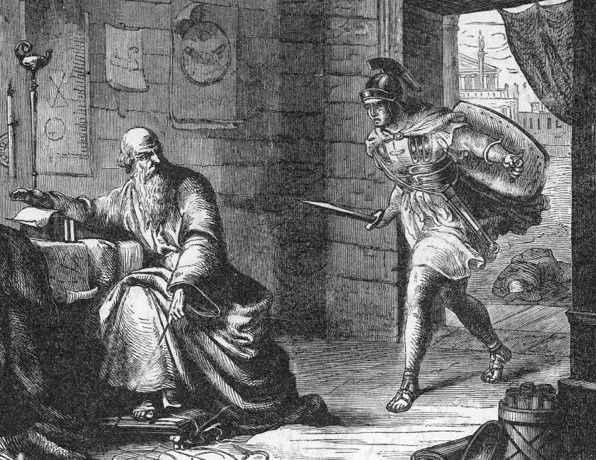
\includegraphics[width= 1\linewidth]{2}
		\caption{\small\textit{\color{quantoan}Hình $2$. Ống xi phông có thể tạo dòng chảy đi lên ngược với chiều của trọng lực nếu hai đầu của chữ U ngược có độ cao khác nhau.}}
		\vspace*{-10pt}
	\end{figure}
	Nếu nhìn lại vào cấu tạo của chiếc cốc Pythagoras, ta có thể thấy ngay một đoạn chữ U ngược tương tự như ống xi phông với một đầu nối với lòng cốc và đầu còn lại nối với chân cốc. Trong thực tế, ống xi phông được sử dụng thường xuyên trong đời sống để tháo nước khỏi các bình chứa, lấy bia ra khỏi thùng bia, rút nước khỏi các mái nhà có diện tích lớn, hay trong khay đựng bột giặt của các máy giặt, ...  Một số nghiên cứu khảo cổ cũng cho thấy ống xi phông đã được sử dụng từ thời Ai Cập cổ đại trong nhiều công việc như dẫn nước thủy lợi hay chế biến đồ uống. 
	\begin{figure}[H]
		\vspace*{-5pt}
		\centering
		\captionsetup{labelformat= empty, justification=centering}
		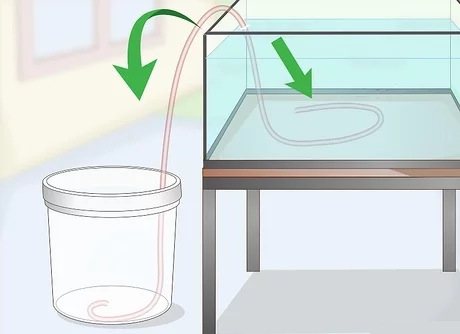
\includegraphics[width= 1\linewidth]{3}
		\caption{\small\textit{\color{quantoan}Hình $3$. Ống xi phông dùng để rút nước khỏi bể chứa.}}
		\vspace*{-10pt}
	\end{figure}
\end{multicols}
%	\newpage
%
%	\setcounter{figure}{0}
%	\thispagestyle{toancuabinone}
\pagestyle{toancuabi}
\everymath{\color{toancuabi}}
\graphicspath{{../toancuabi/pic/}}
\begingroup
\AddToShipoutPicture*{\put(0,616){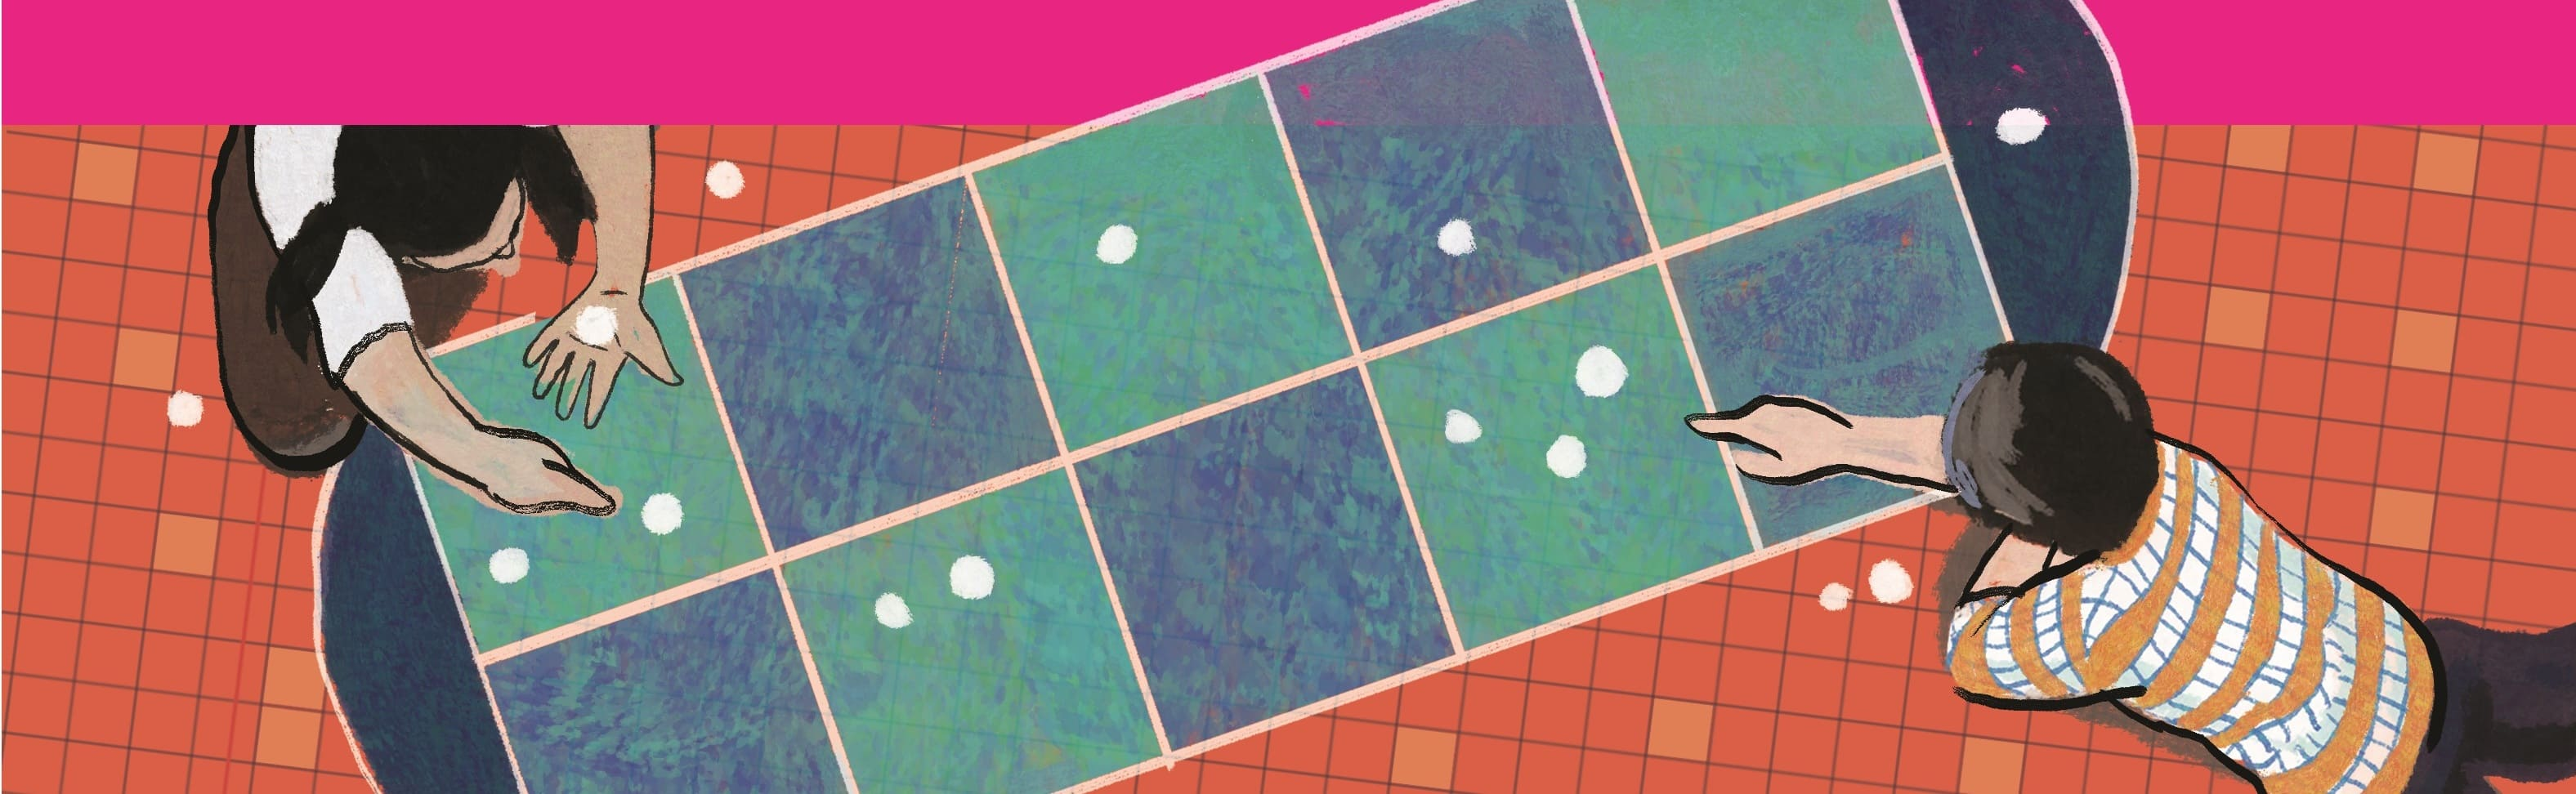
\includegraphics[width=19.3cm]{../bannertoancuabi}}}  
\AddToShipoutPicture*{\put(70,492){
\includegraphics[scale=1]{../tieude1.pdf}}} 
\centering
\endgroup
\vspace*{215pt}

\begin{multicols}{2}
	Trong chương trình phổ thông của Việt Nam, toán tổ hợp đếm được giới thiệu ở cấp THPT. Tuy nhiên trong một số cuộc thi học sinh giỏi toán dành cho cấp tiểu học và đầu cấp PTCS thì phần tổ hợp đếm đã được đưa vào nội dung bài thi khá nhiều, ví dụ như một số cuộc thi khá phổ biến ở Việt Nam hiện nay như IMAS (International Mathematics Assessment), Apmops (The Asia Pacific Mathematical Olympiad for Primary Schools), IMSO (The International Mathematics and Science Olympiad)...
	\vskip 0.1cm
	Trong bài viết này chúng ta cùng làm quen với một số bài toán về đếm tổ hợp trong một số cuộc thi học sinh giỏi cấp tiểu học và lớp $6$ THCS.
	\vskip 0.1cm
	Trước hết chúng ta làm quen với một số khái niệm cơ bản trong phần toán tổ hợp đếm.
	\vskip 0.1cm
	\textbf{\color{toancuabi}Quy tắc cộng, quy tắc nhân:} Quy tắc cộng và quy tắc nhân là hai quy tắc đếm cơ bản, có nội dung có thể được mô tả như sau:
	\vskip 0.1cm
	Có hai công việc gọi là Job $1$ và Job $2$ (có thể mở rộng ra nhiều hơn $2$ công việc) được thực hiện một cách độc lập nhau. Có $m$ cách thực hiện Job $1$ và $n$ cách thực hiện Job $2$, khi đó hai quy tắc đếm cơ bản được phát biểu như sau:
	\vskip 0.1cm
	\textbf{\color{toancuabi}Quy tắc cộng:} Có $m+n$ cách để thực hiện Job $1$ hoặc Job $2$.
	\begin{figure}[H]
		\centering
		\vspace*{-5pt}
		\captionsetup{labelformat=empty, justification=centering}
		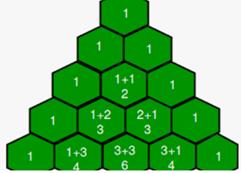
\includegraphics[width=0.85\linewidth]{_1}
		\caption{\small\textit{\color{toancuabi}Quy tắc cộng trong tam giác Pascal.}}
		\vspace*{-10pt}
	\end{figure}
	\textbf{\color{toancuabi}Quy tắc nhân:} Có $m\times n$ cách để thực hiện Job$1$ và Job$2$ (thực hiện cả hai công việc).
	\begin{figure}[H]
		\centering
		\vspace*{-5pt}
		\captionsetup{labelformat=empty, justification=centering}
		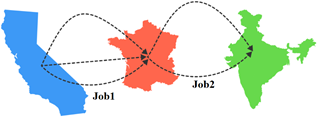
\includegraphics[width=1\linewidth]{_2}
		\caption{\small\textit{\color{toancuabi}Quy tắc nhân trong bài toán đếm đường đi.}}
		\vspace*{-10pt}
	\end{figure}
	\textbf{\color{toancuabi}Giai thừa:} của $n$ là số cách sắp xếp thứ tự của $n$ phần tử trong một tập hợp, được ký hiệu là $n!$ và có công thức là: $n!=1\times 2\times 3\times \ldots\times n $.
	\vskip 0.1cm
	Ghi chú: $0!=1$
	\begin{figure}[H]
		\centering
		\vspace*{5pt}
		\captionsetup{labelformat=empty, justification=centering}
		
\includegraphics[width=1\linewidth]{_3}
		\vspace*{-15pt}
	\end{figure}
	\textbf{\color{toancuabi}Hoán vị (Permutation):} Có $n$ người và chỉ có $k$ cái ghế trên một hàng ($k\le n$), ta cần xếp đủ $k$ người từ nhóm $n$ người vào $k$ cái ghế. Khi đó số cách xếp gọi là hoán vị và ký hiệu là:
	\begin{align*}
		P(n,k)&=n\!\times\!(n\!-\!1)\!\!\times\!\!(n\!-\!2)\!\!\times\!\!\ldots\!\!\times\!\!(n\!-\!k\!+\!1\!)\\
		&= \frac{n!}{(n-k)!} 
	\end{align*}
	\vskip 0.1cm
	Trong trường hợp có $n$ người và có đúng $n$ cái ghế khi đó ta có số cách sắp xếp $n$ người này chính là định nghĩa của $n!$ (số cách sắp xếp các phần tử của một tập hợp $n$ phần tử): $P(n,n)=n!$
	\begin{figure}[H]
		\centering
		\vspace*{-10pt}
		\captionsetup{labelformat=empty, justification=centering}
		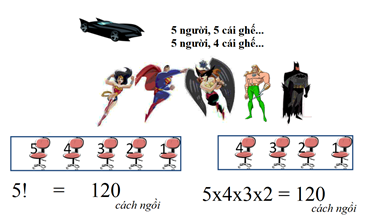
\includegraphics[width=1\linewidth]{_4}
		\vspace*{-15pt}
	\end{figure}
	\resizebox{\columnwidth}{!}{{\textbf{\color{toancuabi}Hoán vị vòng tròn (Circular Permutation):}}} Xung quanh một bàn tròn có $n$ người ngồi. Hai hoán vị được coi là như nhau nếu chúng có thể chồng khít vào nhau bằng phép xuay. Số cách sắp xếp $n$ người xung quanh môt cái bàn tròn cố định là: (\textit{cố định: có nghĩa là ta không thể nhấc nó ra để lật ngược lại được})
	\begin{align*}
		P_n=(n-1)!
	\end{align*}
	Số là $(n-1)!$ thay vì $n!$ vì có $n$ cách xoay bàn và $n$ hoán vị do xoay bàn từ $1$ vị trí là như nhau.
	\begin{figure}[H]
		\centering
		\vspace*{5pt}
		\captionsetup{labelformat=empty, justification=centering}
		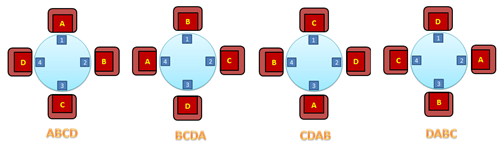
\includegraphics[width=1\linewidth]{_5}
		\caption{\small\textit{\color{toancuabi}Hoán vị vòng tròn $4$ người ngồi xung quanh một cái bàn hình tròn.}}
		\vspace*{-10pt}
	\end{figure}
	\textbf{\color{toancuabi}Tổ hợp (Combonation):}  Đếm số cách để chọn $k$ người từ một nhóm $n$ người là một trong những bài toán tổ hợp đếm cơ bản, và nó được gọi bằng một cái tên đặc biệt: TỔ HỢP và được ký hiệu  $C(n,k)$; $C_n^k$ và có công thức là:
	\begin{align*}
		C_n^k&=C(n,k)=\frac{P(n,k)}{k!} \\[-0.5ex]
		&= \frac{n\!\times\!(n\!-\!1)\!\times\!(n\!-\!2)\!\times\!\ldots \!\times\!(n\!-\!k\!+\!1)}{k!}\\[-0.75ex]
		& = \frac{n!}{k!\times(n-k)!}
	\end{align*}
	\vskip 0.1cm
		\textbf{\color{toancuabi}Bài toán số $\pmb{1}$: (IMAS)}
		\vskip 0.1cm
		Sơ đồ dưới đây gồm nhiều tam giác vuông cân.
		\vskip 0.1cm
		Có bao nhiêu cách một con kiến có thể đi từ $A$ đến $C$ nếu nó chỉ được phép di chuyển lên trên, sang phải hay theo đường chéo? 
		\begin{figure}[H]
			\centering
			\vspace*{-10pt}
			\captionsetup{labelformat=empty, justification=centering}
			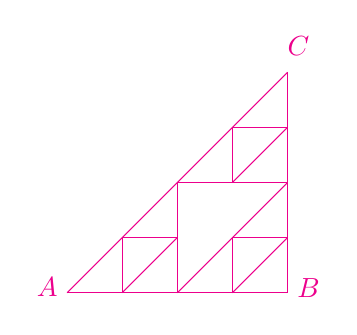
\begin{tikzpicture}[toancuabi,scale=0.7]
				\draw  (-4.,0.)-- (0.,0.);
				\draw  (0.,4.)-- (0.,0.);
				\draw  (0.,4.)-- (-4.,0.);
				\draw  (-3.,0.)-- (-3.,1.);
				\draw  (-3.,1.)-- (-2.,1.);
				\draw  (-2.,0.)-- (-2.,2.);
				\draw  (-2.,2.)-- (0.,2.);
				\draw  (-1.,2.)-- (-1.,3.);
				\draw  (-1.,3.)-- (0.,3.);
				\draw  (0.,1.)-- (-1.,1.);
				\draw  (-1.,1.)-- (-1.,0.);
				\draw  (0.,2.)-- (-2.,0.);
				\draw  (0.,1.)-- (-1.,0.);
				\draw  (-2.,1.)-- (-3.,0.);
				\draw  (0.,3.)-- (-1.,2.);
				\draw (-4.36,0.11) node {$A$};
				\draw (0.38,0.09) node {$B$};
				\draw (0.2,4.47) node {$C$};
			\end{tikzpicture}
			\vspace*{-10pt}
		\end{figure}
	\textbf{\color{toancuabi}Phân tích bài toán:} Tại mỗi điểm nút trên hình vẽ, số cách đi từ $A$ đến nó sẽ bằng tổng số cách đi từ $A$ đến các điểm nút ngay đằng trước nó theo chiều mũi tên được phép đi (phải, lên trên và đi chéo).
	\vskip 0.1cm
	Vậy nên ta có để điền mũi tên hướng đi và áp dụng quy tắc cộng để giải quyết các bài toán dạng này.
	\vskip 0.1cm
	\textit{Lời giải}: Theo quy tắc cộng thể hiện trên hình vẽ bên dưới ta có tổng số cách đi từ $A$ đến $C$ là $42$.
	\begin{figure}[H]
		\centering
%		\vspace*{-10pt}
		\captionsetup{labelformat=empty, justification=centering}
		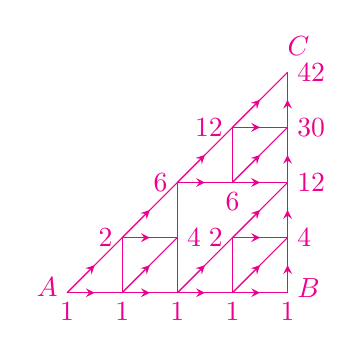
\begin{tikzpicture}[toancuabi,scale=0.7]
			\draw  (-4.,0.)-- (0.,0.);
			\draw  (0.,4.)-- (0.,0.);
			\draw  (0.,4.)-- (-4.,0.);
			\draw  (-3.,0.)-- (-3.,1.);
			\draw  (-3.,1.)-- (-2.,1.);
			\draw  (-2.,0.)-- (-2.,2.);
			\draw  (-2.,2.)-- (0.,2.);
			\draw  (-1.,2.)-- (-1.,3.);
			\draw  (-1.,3.)-- (0.,3.);
			\draw  (0.,1.)-- (-1.,1.);
			\draw  (-1.,1.)-- (-1.,0.);
			\draw  (0.,2.)-- (-2.,0.);
			\draw  (0.,1.)-- (-1.,0.);
			\draw  (-2.,1.)-- (-3.,0.);
			\draw  (0.,3.)-- (-1.,2.);
			
			\draw[-stealth]  (-4.,0.)-- (-3.5,0.);
			\draw[-stealth]  (-3.,0)-- (-2.5,0.);
			\draw[-stealth]  (-2,0)-- (-1.5,0.);
			\draw[-stealth] (-1.,0.)-- (-0.5,0.);
			\draw[-stealth]  (0,0)-- (0,0.5);
			\draw[-stealth]  (0,1)-- (0,1.5);
			\draw[-stealth]  (0,2)-- (0,2.5);
			\draw[-stealth]  (0,3)-- (0,3.5);
			\draw[-stealth]  (-3,1)-- (-2.5,1);
			\draw[-stealth]  (-1,1)-- (-0.5,1);
			\draw[-stealth]  (-2,2)-- (-1.5,2);
			\draw[-stealth]  (-1,2)-- (-0.5,2);
			\draw[-stealth]  (-1,3)-- (-0.5,3);
			
			\draw[-stealth]  (-4,0)-- (-3.5,0.5);
			\draw[-stealth]  (-3,1)-- (-2.5,1.5);
			\draw[-stealth]  (-2.,2.)-- (-1.5,2.5);
			\draw[-stealth]  (-1.,3.)-- (-0.5,3.5);
			\draw[-stealth]  (-3,0)-- (-2.5,0.5);
			\draw[-stealth]  (-2,0)-- (-1.5,0.5);
			\draw[-stealth]  (-1,0)-- (-0.5,0.5);
			\draw[-stealth]  (-1,1)-- (-0.5,1.5);
			\draw[-stealth]  (-1,2)-- (-0.5,2.5);
			
			\draw (-4.36,0.11) node {$A$};
			\draw (0.38,0.09) node {$B$};
			\draw (0.2,4.47) node {$C$};
			
			\draw (-4,0) node[below]{$1$};
			\draw (-3,0) node[below]{$1$};
			\draw (-2,0) node[below] {$1$};
			\draw (-1,0) node[below] {$1$};
			\draw (0,0) node[below] {$1$};
			\draw (-3,1) node[left] {$2$};
			\draw (-2,1) node[right] {$4$};
			\draw (-1,1) node[left] {$2$};
			\draw (0,1) node[right] {$4$};
			\draw (-2,2) node[left] {$6$};
			\draw (-1,2) node[below] {$6$};
			\draw (0,2) node[right] {$12$};
			\draw (0,3) node[right] {$30$};
			\draw (0,4) node[right] {$42$};
			\draw (-1,3) node[left] {$12$};
		\end{tikzpicture}
		\vspace*{-10pt}
	\end{figure}
	\textbf{\color{toancuabi}Bài toán số $\pmb{2}$: (IMAS)}
	\vskip 0.1cm
	$8$ ký tự $2,0,1,5,I,M,A,S$ được xếp trên $1$ hàng. Hỏi có bao nhiêu cách xếp sao cho các chữ số đứng đằng trước các chữ cái, chữ số $0$ không đứng đầu tiên.
	\vskip 0.1cm
	\textit{Lời giải.}
	Có $8$ vị trí để xếp $8$ ký tự, các chữ số đứng đằng trước các chữ cái nên $4$ vị trí đầu tiên là các chữ số và $4$ vị trí sau cùng. Ta thực hiện $2$ công việc là xếp chữ số và xếp chữ cái:
	\vskip 0.1cm
	+ Có $3\times3\times2\times1=18$ cách xếp các chữ số (chữ số $0$ không đứng ở đầu nên vị trí đầu chỉ có $3$ cách chọn chữ số).
	\vskip 0.1cm
	+ Có $4\times3\times2\times1=4!=24$ cách xếp $4$ chữ cái.
	\vskip 0.1cm
	Theo quy tắc nhân (hai quy tắc cơ bản trong đếm tổ hợp là quy tắc cộng và quy tắc nhân) ta có số cách xếp $8$ ký tự là: $18\times24=432$.
	\vskip 0.1cm
	(Ta có thể lập luận: ta thực hiện $3$ công việc theo thứ tự là Job $1$ là viết chữ số đầu tiên, Job $2$ là viết $3$ chữ số tiếp theo, Job $3$ là viết $4$ chữ cái, và theo quy tắc nhân ta có kết quả là: $P(3,1)\times P(3,3)\times P(4,4)=3\times3!\times4!=432$)
	\vskip 0.1cm
	Mở rộng bài toán số $2$, các bạn thử sức với bài toán số $3$ nhé.
	\vskip 0.1cm
	\textbf{\color{toancuabi}Bài toán số $\pmb{3}$:}
	\vskip 0.1cm
	$8$ ký tự $2,0,1,5,I,M,A,S$ được xếp trên $1$ hàng. Hỏi có bao nhiêu cách xếp thỏa mãn một trong các điều kiện sau:
	\vskip 0.1cm
	$a)$ Không có hai chữ cái nào đứng cạnh nhau.
	\vskip 0.1cm
	$b)$ Chữ số $0$ nằm giữa hai chữ cái $I$ và $S$.
	\vskip 0.1cm
	$c)$ Chữ số $0$ và chữ số $1$ không đứng cạnh nhau.
	\vskip 0.1cm
	$d)$ $4$ chữ cái luôn đứng cạnh nhau.
	\vskip 0.1cm
	\textbf{\color{toancuabi}Bài toán số $4$: (IMAS)}
	\vskip 0.1cm
	Có bao nhiêu số có $3$ chữ số không chứa chữ số $3$ và chia hết cho $3$.
	\vskip 0.1cm
	\textbf{\color{toancuabi}Phân tích bài toán:}
	\vskip 0.1cm
	Gọi số có $3$ chữ số là $\overline{abc}$:
	\vskip 0.1cm
	Thử từ số nhỏ để tìm quy luật:
	\begin{align*}
		&102, 105, 108,111, 114, 117\\
		&120, 126, 129,132, 135, 138\\
		&141, 144, 147,150, 156, 159...
	\end{align*}
	Ta nhận thấy chữ số $c$ lặp theo nhóm $(2,5,8)$, $(1,4,7)$, $(0,6,9)$ và mỗi nhóm này xuất hiện phụ thuộc vào số dư chi $3$ của số $\overline{ab}$ từ đó ta có lời giải như sau:
	\vskip 0.1cm
	\textit{Lời giải}.
	Nếu $\overline{ab}$ chia $3$ dư $0$ ta có $3$ cách chọn $c=\{0,6,7\}$
	\vskip 0.1cm
	Nếu $\overline{ab}$ chia $3$ dư $1$ ta có $3$ cách chọn $c=\{2,5,8\}$
	\vskip 0.1cm
	Nếu $\overline{ab}$ chia $3$ dư $2$ ta có $3$ cách chọn $c=\{1,4,7\}$
	\vskip 0.1cm
	Vậy mỗi số $\overline{ab}$ ta luôn có $3$ cách chọn chữ số $c$.
	\vskip 0.1cm
	Ta có $9\times 10$ cách tạo ra số $\overline{ab}$.
	\vskip 0.1cm
	Vậy số số có $3$ chữ số không chứa chữ số $3$ và chia hết cho $3$ là: $9\times10\times3=270$ (số);
	\vskip 0.1cm
	\textbf{\color{toancuabi}Bài toán số $5$: (APMOPS)}
	\vskip 0.1cm
	Mỗi cạnh của hình ngũ giác có cạnh $a,$ $b,$ $c,$ $d,$ $e$ tương ứng được tô bằng một trong $3$ mầu xanh, đỏ, vàng. Hỏi có bao nhiêu cách tô mầu cách cạnh của hình ngũ giác này sao cho không có $2$ cạnh nào kề nhau có cùng mầu.
	\begin{figure}[H]
		\centering
		\vspace*{-10pt}
		\captionsetup{labelformat=empty, justification=centering}
		\begin{tikzpicture}[toancuabi, scale=0.75]
			\draw  (-5.,3.)-- (-3.,4.);
			\draw  (-3.,4.)-- (-1.,4.);
			\draw  (-1.,4.)-- (0.,2.);
			\draw  (0.,2.)-- (-3.,0.);
			\draw  (-3.,0.)-- (-5.,3.);
			\draw (-4.08,3.89) node {$e$};
			\draw (-2.,4.35) node {$a$};
			\draw (-0.32,3.21) node {$b$};
			\draw (-1.2,0.95) node {$c$};
			\draw (-4.2,1.39) node {$d$};
		\end{tikzpicture}
		\vspace*{-10pt}
	\end{figure}
	\textbf{\color{toancuabi}Phân tích bài toán:} Nếu ta tô thứ tự $a,$ $b,$ $c,$ $d,$ $e$ thì $a$ và $b$ có tương ứng $3$ và $2$ cách tô. Đến tô $c$ thông thường sẽ có $2$ cách tô, $d$ cũng $2$ cách tô, nhưng nếu như vậy thì $e$ sẽ không xác định được số cách tô vì nó phụ thuộc vào $2$ cạnh $a$ và $d$, bởi vậy ta cần xét đến mầu cụ thể của $c$ cũng như của $d$ để tính được số cách tô mầu $c$. Vậy ta có thể tiếp cận bài toán bằng hai cách sau đây.
	\vskip 0.1cm
	\textit{Lời giải $1$:}
	Tô $a$, có $3$ cách tô, tô $b$, có $2$ cách tô.
	\vskip 0.1cm
	Tô $c$:
	\vskip 0.1cm
	\textbf{\color{toancuabi}Trường hợp $\pmb{1}$:} $c$ cùng mầu với $a, c$ có $1$ cách tô, $d$ có $2$ cách tô, $e$ có $1$ cách tô, số cách tô ngũ giác là: $3\times2\times1\times2\times1=12$.  \hfill($1$)
	\vskip 0.1cm
	\textbf{\color{toancuabi}Trường hợp $\pmb{2}$:} $c$ khác mầu với $a, c$ có $1$ cách tô (vì $c$ khác với cạnh $b$ kề với nó), xét $2$ khả năng tô $d$:
	\vskip 0.1cm
	$2.1$ $d$ cùng mầu với $a, d$ có $1$ cách tô, e có $2$ cách tô. Số cách tô ngũ giác là $3\times2\times1\times2\times1=12$. \hfill($2$)
	\vskip 0.1cm
	$2.2$ $d$ khác mầu $a, d$ có $1$ cách tô (vì $c$ khác mầu $a$), $e$ có $1$ cách tô. Số cách tô ngũ giác là: $3\times2\times1\times1\times1=6$. \hfill($3$)
	\vskip 0.1cm
	Từ ($1$),($2$),($3$) ta có số cách tô cần tìm là: $12+12+6=30$.
	\vskip 0.1cm
	\textit{Lời giải $2$:}
	Tô $a$, có $3$ cách tô. Tô $c$, xét $2$ trường hợp:
	\vskip 0.1cm
	\textbf{\color{toancuabi}Trường hợp $\pmb{1}$:} $c$ cùng mầu $a, c$ có $1$ cách tô, $b$ có $2$ cách tô, $d$ có $2$ cách tô, $e$ có $1$ cách tô. Số cách tô ngũ giác là: 
	$3\times1\times2\times2$ \linebreak$\times1=12$. \hfill ($1$)
	\vskip 0.1cm
	\textbf{\color{toancuabi}Trường hợp $\pmb{2}$:} $c$ khác mầu $a, c$ có $2$ cách tô, $b$ có $1$ cách tô. Xét $2$ khả năng tô $d$.
	\vskip 0.1cm
	$2.1$ $d$ cùng mầu với $a, d$ có $1$ cách tô, $e$ có $2$ cách tô. Số cách tô ngũ giác là: $3\times2\times1\times1\times2=12$. \hfill ($2$)
	\vskip 0.1cm
	$2.2$ $d$ khác mầu $a$, $d$ có $1$ cách tô (do $c$ khác mầu $a$), $e$ có $1$ cách tô. Số cách tô ngũ giác là: $3\times2\times1\times1\times1=6$.\hfill ($3$)
	\vskip 0.1cm
	Từ ($1$),($2$),($3$) ta có số cách tô cần tìm là: $12+12+6=30$.
	\vskip 0.1cm
		\textbf{\color{toancuabi}Bài toán số $\pmb{6}$: (Apmops)}
		\vskip 0.1cm
		$A,B,C,D,E$ và $F$ là các điểm nằm trên $2$ đường thẳng như hình vẽ. Có bao nhiêu tam giác được tạo bởi $3$ trong $6$ điểm đã cho.
		\begin{figure}[H]
			\centering
			\vspace*{-5pt}
			\captionsetup{labelformat=empty, justification=centering}
			\begin{tikzpicture}[toancuabi]
				\draw  (-5.,2.)-- (-0.02,2.58);
				\draw  (-4.94,2.78)-- (-0.66,5.62);
				\draw[fill=white]  (-3.9971801091570645,3.4056094602789573) circle (1.5pt);
				\draw (-3.86,3.77) node {$A$};
				\draw[fill=white]  (-2.7676858702243776,4.221442086112797) circle (1.5pt);
				\draw (-2.62,4.59) node {$B$};
				\draw[fill=white]  (-1.6167058823529414,4.985176470588236) circle (1.5pt);
				\draw (-1.48,5.35) node {$C$};
				\draw[fill=white]  (-3.7559113331848124,2.144893860793737) circle (1.5pt);
				\draw (-3.62,2.51) node {$F$};
				\draw[fill=white]  (-2.1392062633270745,2.3331848127048787) circle (1.5pt);
				\draw (-2.,2.71) node {$E$};
				\draw[fill=white]  (-0.8951175965118869,2.4780786734986155) circle (1.5pt);
				\draw (-0.76,2.85) node {$D$};
			\end{tikzpicture}
			\vspace*{-5pt}
		\end{figure}
	\vskip 0.1cm
	\textbf{\color{toancuabi}Phân tích bài toán:}
	\vskip 0.1cm
	Trên mặt phẳng cứ $3$ điểm phân biệt không thẳng hàng luôn tạo ra một tam giác, còn $3$ điểm phân biệt thẳng hàng thì không tạo ra một tam giác thông thưởng mà thường được gọi là tam giác suy biến (degenerate triangle). Tương tự như thế, nếu có các đường thẳng đôi một cắt nhau, mà không có $3$ đường thẳng nào cắt nhau tại $1$ điểm ($3$ đường đồng quy) thì cứ $3$ đường thẳng tạo ra được $1$ đoạn thẳng. Cứ $3$ đường thẳng đồng quy thì nó tạo ra một tam giác suy biến (có $3$ đỉnh trùng vào nhau). Các tính chất này có thể được áp dụng để giải bài toán trên và các bài toán mở rộng ở phần dưới.
	\vskip 0.1cm
	\textit{Lời giải $1$:}
	Xét $2$ trường hợp, trường hợp $1$: tam giác có đáy nằm ở đường thẳng phía dưới, đỉnh nằm ở đường thẳng phía trên, có $C(3,2)$ cách chọn đáy và $C(3,1)$ cách chọn đỉnh, theo quy tắc nhân, số tam giác đếm được là: $C(3,2)\times C(3,1)$. Tương tự, trường hợp $2$: tam giác có đáy nằm ở đường thẳng phía trên, đỉnh nằm ở đường thẳng phía dưới, có $C(3,2)$ cách chọn đáy và $C(3,1)$ cách chọn đỉnh, theo quy tắc nhân, số tam giác đếm được là: $C(3,2)\times C(3,1)$.
	\vskip 0.1cm
	Vậy số tam giác cần tìm là: $2\times C(3,2)\times C(3,1) = 2\times3\times3=18$.
	\vskip 0.1cm
	\textit{Lời giải $2$:}
	Số cách chọn ra $3$ điểm là: $C(6,3)=6\times 5\times4/3!=20$
	\vskip 0.1cm
	Số tam giác suy biến là: $3\times C(3,3)=2$
	\vskip 0.1cm
	Vậy số tam giác là: $20-2=18$
	\vskip 0.1cm
	Mở rộng bài toán số $5$, các bạn thử sức của mình xem sao nhé.
	\vskip 0.1cm
		\textbf{\color{toancuabi}Bài toán $\pmb{6.1}$ (Apmops)}
		\vskip 0.1cm
		Cho các điểm $A1$, $A2$, $A3$, $B1$, $B2$, $B3$, $B4$, $C1$, $C2$, $C3$, $C4$ và $C5$ nằm trên $3$ đường thẳng như hình vẽ. Có bao nhiêu tam giác được tạo bởi $3$ trong các đỉnh đã cho?
		\begin{figure}[H]
			\centering
			\vspace*{-5pt}
			\captionsetup{labelformat=empty, justification=centering}
			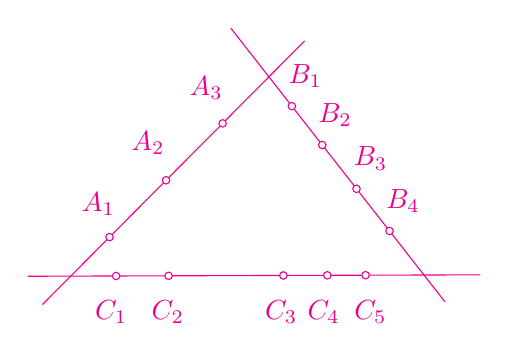
\begin{tikzpicture}[toancuabi, scale=0.9]
				\draw  (-5.4,1.6)-- (-1.7,5.32);
				\draw  (-2.74,5.5)-- (0.28,1.64);
				\draw  (-5.6,2.)-- (0.78,2.02);
				\draw[fill=white]  (-4.45248688627018,2.552634806236469) circle (1.5pt);
				\draw (-4.61,3.02) node {$A_1$};
				\draw[fill=white]  (-3.6547027796748095,3.3547312593539766) circle (1.5pt);
				\draw (-3.91,3.88) node {$A_2$};
				\draw[fill=white]  (-2.856811147760132,4.1569358190087335) circle (1.5pt);
				\draw (-3.09,4.66) node {$A_3$};
				\draw[fill=white]  (-1.8796143213988348,4.400301748542881) circle (1.5pt);
				\draw (-1.69,4.82) node {$B_1$};
				\draw[fill=white]  (-1.4504776019983348,3.851802497918401) circle (1.5pt);
				\draw (-1.27,4.28) node {$B_2$};
				\draw[fill=white]  (-0.9673278934221485,3.2342667776852623) circle (1.5pt);
				\draw (-0.77,3.66) node {$B_3$};
				\draw[fill=white]  (-0.5014784346378021,2.6388432972522895) circle (1.5pt);
				\draw (-0.31,3.06) node {$B_4$};
				\draw[fill=white]  (-4.359949489986439,2.003887305674024) circle (1.5pt);
				\draw (-4.43,1.5) node {$C_1$};
				\draw [fill=white] (-3.619831371238773,2.0062074251685305) circle (1.5pt);
				\draw (-3.63,1.5) node {$C_2$};
				\draw[fill=white]  (-2.0000353766631944,2.0112851555590496) circle (1.5pt);
				\draw (-2.03,1.5) node {$C_3$};
				\draw[fill=white]  (-1.3800414693107446,2.0132287101275526) circle (1.5pt);
				\draw (-1.43,1.5) node {$C_4$};
				\draw[fill=white]  (-0.839921385192901,2.0149218765354453) circle (1.5pt);
				\draw (-0.77,1.5) node {$C_5$};
			\end{tikzpicture}
			\vspace*{-15pt}
		\end{figure}
		\textbf{\color{toancuabi}Bài toán $\pmb{6.2}$}
		Có bao nhiêu tam giác trong hình vẽ?
		\begin{figure}[H]
			\centering
			\vspace*{-10pt}
			\captionsetup{labelformat=empty, justification=centering}
			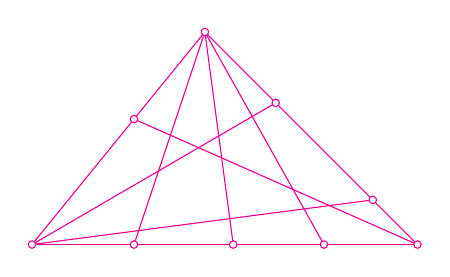
\begin{tikzpicture}[toancuabi,scale=0.9]
				\draw  (1.,3.)-- (-1.44,0.);
				\draw  (-1.44,0.)-- (4.,0.);
				\draw  (4.,0.)-- (1.,3.);
				\draw  (1.,3.)-- (0.,0.);
				\draw  (1.,3.)-- (1.4,0.);
				\draw  (1.,3.)-- (2.68,0.);
				\draw  (4.,0.)-- (0.,1.7704918032786887);
				\draw  (-1.44,0.)-- (2.,2.);
				\draw  (-1.44,0.)-- (3.37,0.63);
					\draw [fill=white] (1.,3.) circle (1.5pt);
					\draw [fill=white] (-1.44,0.) circle (1.5pt);
					\draw [fill=white] (4.,0.) circle (1.5pt);
					\draw [fill=white] (0.,0.) circle (1.5pt);
					\draw [fill=white] (1.4,0.) circle (1.5pt);
					\draw [fill=white] (2.68,0.) circle (1.5pt);
					\draw [fill=white] (0.,1.7704918032786887) circle (1.5pt);
					\draw [fill=white] (2.,2.) circle (1.5pt);
					\draw [fill=white] (3.37,0.63) circle (1.5pt);
			\end{tikzpicture}
			\vspace*{-5pt}
		\end{figure}
		\textbf{\color{toancuabi}Bài toán $\pmb{6.3}$}
		Có bao nhiêu tam giác được tạo bởi $3$ trong $12$ điểm đã cho trên lưới ô vuông như hình vẽ?
		\begin{figure}[H]
			\centering
			\vspace*{-5pt}
			\captionsetup{labelformat=empty, justification=centering}
			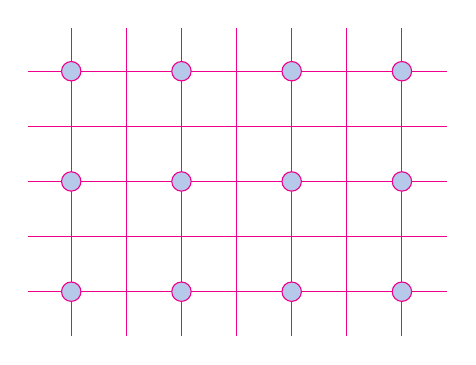
\begin{tikzpicture}[toancuabi,scale=0.7]
				\draw [xstep=1.0cm,ystep=1.0cm] (-2.78,-0.8) grid (4.82,4.78);
					\draw [fill=cackithi!40] (-2.,4.) circle (5.0pt);
					\draw [fill=cackithi!40] (0.,4.) circle (5.0pt);
					\draw [fill=cackithi!40] (2.,4.) circle (5.0pt);
					\draw [fill=cackithi!40] (4.,4.) circle (5.0pt);
					\draw [fill=cackithi!40] (4.,2.) circle (5.0pt);
					\draw [fill=cackithi!40] (4.,0.) circle (5.0pt);
					\draw [fill=cackithi!40] (2.,0.) circle (5.0pt);
					\draw [fill=cackithi!40] (2.,2.) circle (5.0pt);
					\draw [fill=cackithi!40] (0.,2.) circle (5.0pt);
					\draw [fill=cackithi!40] (0.,0.) circle (5.0pt);
					\draw [fill=cackithi!40] (-2.,2.) circle (5.0pt);
					\draw [fill=cackithi!40] (-2.,0.) circle (5.0pt);
			\end{tikzpicture}
			\vspace*{-5pt}
		\end{figure}
	\textbf{\color{toancuabi}Bài toán số $\pmb{7}$: (Apmops)}
	\vskip 0.1cm
	Có bao nhiêu cách để tô $6$ mặt của một hình lập phương bằng $6$ mầu, mỗi mặt được tô bằng $1$ mầu sao cho không có hai mặt nào có cùng mầu? (Hai cách tô mầu được coi là như nhau nếu chúng nhìn giống hệt nhau sau một phép xoay hình). 
	\vskip 0.1cm
	\textbf{\color{toancuabi}Phân tích bài toán:} Hướng đi thứ nhất, ta hình dung nếu cố định hình lập phương lại và mỗi cách nhìn khác nhau ở mỗi phía được coi là khác nhau, như thế thì số cách tô sẽ như tô theo hàng ngang ($6$ người ngồi trên $6$ cái ghế trên $1$ hàng) và sẽ là $6!=720$ cách. Do hình lập phương này xoay được nên ta xem mỗi một kiểu tô có bao nhiêu cách xoay nó xung quanh chính nó. Do có $6$ mầu ta có $6$ cách xuay để có đáy khác mầu. Mỗi cách đặt đáy với $1$ mầu ta có $4$ cách xoay xung quanh chính nó (do hình lập phương có $4$ cạnh bên), từ đó ta có hướng giải quyết bài toán.
	\vskip 0.1cm
	Hướng đi thứ $2$, do hình lập phương xoay được nên ta có thể cố định mầu ở những vị trí ta có thể xuay nó về và ta sẽ có hướng giải quyết bài toán như lời giải $2$.
	\vskip 0.1cm
	Hướng đi thứ $3$ gần giống với hướng thứ $2$, ta có thể hình dung mình có thể tô mầu ở đáy bằng mầu tùy thích do hình lập phương xoay được, mặt đối diện trên đỉnh sẽ còn $5$ cách tô, $4$ mặt xung quanh ta sẽ hình dung nó như $4$ người ngồi xung quanh một cái bàn tròn nên ta có thể áp dụng bài toán hoán vị vòng tròn để giải quyết.
	\vskip 0.1cm
	\textit{Lời giải $1$:}
	Giả sử hình lập phương cố định, khi đó ta có $6!=720$ cách tô.
	\vskip 0.1cm
	Mỗi cách tô ta có $6$ cách đặt các mặt khác mầu nhau xuống đáy, khi đặt rồi ta có $4$ cách xoay xung quanh nó, vậy ứng với mỗi cách tô mầu ta có $6\times4=24$ cách xoay nó xung quanh chính nó. Vậy số cách tô mầu là: $720:24=30$ (cách).
	\vskip 0.1cm
	\textit{Lời giải $2$:}
	Đầu tiên ta tô mầu $1$ mặt (mầu ta thích), rồi đặt nó xuống đáy, khi đó ở mặt đối diện trên đỉnh có $5$ cách tô.
	\vskip 0.1cm
	Tiếp theo ta tô mầu $1$ mặt xung quanh (mầu ta thích trong $4$ mầu còn lại), rồi xoay nó sang bên trái, khi đó mặt bên phải có $3$ cách tô, còn $2$ mặt còn lại (trước và sau) có $2!$ cách tô, vậy số cách tô mầu là: $1\times5\times1\times3\times2!=30$ (cách)
	\vskip 0.1cm
	\textit{Lời giải $3$:}
	Tương tự như lời giải $2$, đầu tiên ta tô mầu $1$ mặt (mầu ta thích), rồi đặt nó xuống đáy, khi đó ở mặt đối diện trên đỉnh có $5$ cách tô.
	\vskip 0.1cm
	Còn $4$ mặt xung quanh, do xoay được nên theo bài toán hoán vị vòng tròn ta có $4!/4=6$ cách tô.
	\vskip 0.1cm
	Vậy số cách tô mầu hình lập phương là: $5\times 6=30$ (cách).
	\vskip 0.1cm
	\textbf{\color{toancuabi}Bài toán số $\pmb{8}$: (IMSO)}
	\vskip 0.1cm
	Một hình lập phương được tô các mặt bằng $6$ mầu, mỗi mặt $1$ mầu khác nhau và được đánh số từ $1$ đến $6$ sao cho tổng hai mặt đối diện bằng $7$. Hỏi có bao nhiêu cách tô mầu và đánh số hình lập phương này? (Hai cách tô mầu, đánh số được coi là như nhau nếu chúng nhìn giống hệt nhau sau một phép xoay hình). 
	\vskip 0.1cm
	Phân tích bài toán: Bài toán này là tương đối khó khi các bạn lớp $5,6$ đi thi gặp phải, và đúng là trong năm thi đó đoàn học sinh Việt Nam chỉ có đúng $1$ bạn làm được, tuy nhiên nếu chia bài toán làm hai bước, bước $1$ tô mầu, bước $2$ điền số thì ta có thể giải quyết được bài toán một cách tương đối dễ dàng.
	\vskip 0.1cm
	\textit{Lời giải:}
	Bước $1$: Tô mầu hình lập phương, theo bài toán số $7$, ta có $30$ cách tô mầu hình lập phương này.
	\vskip 0.1cm
	Bước $2$: Đánh số, ta đánh theo thứ tự:
	\vskip 0.1cm
	Đánh số $1$, có $6$ cách. Đánh số $6$ ở mặt đối diện số $1$, có $1$ cách.
	\vskip 0.1cm
	Đánh số $2$, có $4$ cách (do còn $4$ mặt chưa đánh số). Đánh số $5$ ở mặt đối diện, có $1$ cách.
	\vskip 0.1cm
	Đánh số $3$, có $2$ cách (do còn $2$ mặt chưa đánh số). Đánh số $4$ ở mặt đối diện, có $1$ cách.
	\vskip 0.1cm
	Vậy ta có $6\times1\times4\times1\times2\times1=48$ cách đánh số.
	\vskip 0.1cm
	Theo quy tắc nhân ta có số cách tô mầu và đánh số là: $30\times 48=1440$ (cách).
	\vskip 0.1cm
	\textbf{\color{toancuabi}Bài toán số $\pmb{9}$: (IMAS)}
	\vskip 0.1cm
		Một bàn cờ hình vuông $5\times 5$ được xếp một hình chữ L chiếm $4$ ô như hình vẽ. Ta có thể xuay hoặc lật hình chữ L này. Hỏi có bao nhiêu cách xếp hình chữ L này vào bàn cờ hình vuông đã cho?
		\begin{figure}[H]
			\centering
			\vspace*{-5pt}
			\captionsetup{labelformat=empty, justification=centering}
			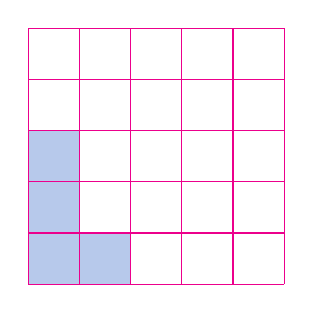
\begin{tikzpicture}[toancuabi,scale=0.65]
				\filldraw[cackithi!40] (0,0) rectangle (1,3);
				\filldraw[cackithi!40] (1,0) rectangle (2,1);
				\draw (0,0) grid (5,5);
			\end{tikzpicture}
			\vspace*{-10pt}
		\end{figure}
	\textbf{\color{toancuabi}Phân tích bài toán:} Ta nhận thấy hình chữ L tô đen có thể xoay hoặc lật được, nên ta sẽ xem nó có thể có bao nhiêu cách biến hình (xoay hoặc lật).  Ứng với mỗi phép biến hình bằng xoay, lật ta xem có bao nhiêu cách trượt nó theo hàng ngang và hàng dọc, từ đó ta có cách giải quyết bài toán.
	\vskip 0.1cm
	\textit{Lời giải:}
	Ta tính số cách xoay, lật hình chữ L tô đậm, như hình dưới ta có $8$ cách.
	\begin{figure}[H]
		\centering
		\vspace*{-5pt}
		\captionsetup{labelformat=empty, justification=centering}
		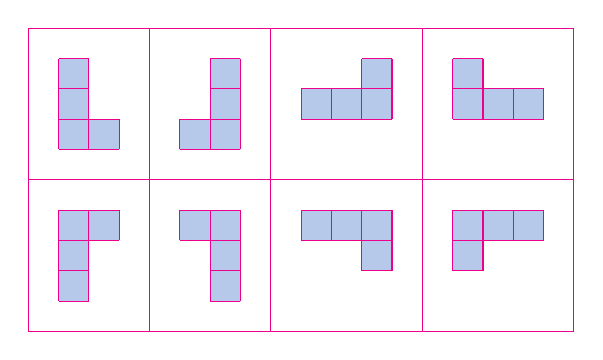
\begin{tikzpicture}[toancuabi,scale=0.385]
			\fill[cackithi!40] (1.,3.) -- (2.,3.) -- (2.,1.) -- (3.,1.) -- (3.,0.) -- (1.,0.) -- cycle;
			\fill[cackithi!40] (5.,0.) -- (7.,0.) -- (7.,3.) -- (6.,3.) -- (6.,1.) -- (5.,1.) -- cycle;
			\fill[cackithi!40] (9.,2.) -- (11.,2.) -- (11.,3.) -- (12.,3.) -- (12.,1.) -- (9.,1.) -- cycle;
			\fill[cackithi!40] (14.,3.) -- (14.,1.) -- (17.,1.) -- (17.,2.) -- (15.,2.) -- (15.,3.) -- cycle;
			\fill[cackithi!40] (3.,-2.) -- (1.,-2.) -- (1.,-5.) -- (2.,-5.) -- (2.,-3.) -- (3.,-3.) -- cycle;
			\fill[cackithi!40] (5.,-2.) -- (7.,-2.) -- (7.,-5.) -- (6.,-5.) -- (6.,-3.) -- (5.,-3.) -- cycle;
			\fill[cackithi!40] (9.,-2.) -- (12.,-2.) -- (12.,-4.) -- (11.,-4.) -- (11.,-3.) -- (9.,-3.) -- cycle;
			\fill[cackithi!40] (14.,-2.) -- (14.,-4.) -- (15.,-4.) -- (15.,-3.) -- (17.,-3.) -- (17.,-2.) -- cycle;
			\draw [] (1.,3.)-- (2.,3.);
			\draw [] (2.,3.)-- (2.,1.);
			\draw [] (2.,1.)-- (3.,1.);
			\draw [] (3.,1.)-- (3.,0.);
			\draw [] (3.,0.)-- (1.,0.);
			\draw [] (1.,0.)-- (1.,3.);
			\draw [] (5.,0.)-- (7.,0.);
			\draw [] (7.,0.)-- (7.,3.);
			\draw [] (7.,3.)-- (6.,3.);
			\draw [] (6.,3.)-- (6.,1.);
			\draw [] (6.,1.)-- (5.,1.);
			\draw [] (5.,1.)-- (5.,0.);
			\draw [] (9.,2.)-- (11.,2.);
			\draw [] (11.,2.)-- (11.,3.);
			\draw [] (11.,3.)-- (12.,3.);
			\draw [] (12.,3.)-- (12.,1.);
			\draw [] (12.,1.)-- (9.,1.);
			\draw [] (9.,1.)-- (9.,2.);
			\draw [] (14.,3.)-- (14.,1.);
			\draw [] (14.,1.)-- (17.,1.);
			\draw [] (17.,1.)-- (17.,2.);
			\draw [] (17.,2.)-- (15.,2.);
			\draw [] (15.,2.)-- (15.,3.);
			\draw [] (15.,3.)-- (14.,3.);
			\draw [] (3.,-2.)-- (1.,-2.);
			\draw [] (1.,-2.)-- (1.,-5.);
			\draw [] (1.,-5.)-- (2.,-5.);
			\draw [] (2.,-5.)-- (2.,-3.);
			\draw [] (2.,-3.)-- (3.,-3.);
			\draw [] (3.,-3.)-- (3.,-2.);
			\draw [] (5.,-2.)-- (7.,-2.);
			\draw [] (7.,-2.)-- (7.,-5.);
			\draw [] (7.,-5.)-- (6.,-5.);
			\draw [] (6.,-5.)-- (6.,-3.);
			\draw [] (6.,-3.)-- (5.,-3.);
			\draw [] (5.,-3.)-- (5.,-2.);
			\draw [] (9.,-2.)-- (12.,-2.);
			\draw [] (12.,-2.)-- (12.,-4.);
			\draw [] (12.,-4.)-- (11.,-4.);
			\draw [] (11.,-4.)-- (11.,-3.);
			\draw [] (11.,-3.)-- (9.,-3.);
			\draw [] (9.,-3.)-- (9.,-2.);
			\draw [] (14.,-2.)-- (14.,-4.);
			\draw [] (14.,-4.)-- (15.,-4.);
			\draw [] (15.,-4.)-- (15.,-3.);
			\draw [] (15.,-3.)-- (17.,-3.);
			\draw [] (17.,-3.)-- (17.,-2.);
			\draw [] (17.,-2.)-- (14.,-2.);
			\draw  (0.,4.)-- (18.,4.);
			\draw  (18.,4.)-- (18.,-6.);
			\draw  (18.,-6.)-- (0.,-6.);
			\draw  (0.,4.)-- (0.,-6.);
			\draw  (0.,-1.)-- (18.,-1.);
			\draw  (13.,4.)-- (13.,-6.);
			\draw  (8.,4.)-- (8.,-6.);
			\draw  (4.,4.)-- (4.,-6.);
			\draw  (1.,2.)-- (2.,2.);
			\draw  (1.,1.)-- (2.,1.);
			\draw  (2.,1.)-- (2.,0.);
			\draw  (6.,2.)-- (7.,2.);
			\draw  (6.,1.)-- (7.,1.);
			\draw  (6.,1.)-- (6.,0.);
			\draw  (11.,2.)-- (11.,1.);
			\draw  (10.,2.)-- (10.,1.);
			\draw  (11.,2.)-- (12.,2.);
			\draw  (15.,2.)-- (15.,1.);
			\draw  (15.,2.)-- (14.,2.);
			\draw  (16.,2.)-- (16.,1.);
			\draw  (15.,-2.)-- (15.,-3.);
			\draw  (16.,-2.)-- (16.,-3.);
			\draw  (15.,-3.)-- (14.,-3.);
			\draw  (11.,-3.)-- (12.,-3.);
			\draw  (11.,-3.)-- (11.,-2.);
			\draw  (10.,-2.)-- (10.,-3.);
			\draw  (6.,-3.)-- (7.,-3.);
			\draw  (7.,-4.)-- (6.,-4.);
			\draw  (6.,-3.)-- (6.,-2.);
			\draw  (2.,-3.)-- (2.,-2.);
			\draw  (2.,-3.)-- (1.,-3.);
			\draw  (1.,-4.)-- (2.,-4.);
		\end{tikzpicture}
		\vspace*{-10pt}
	\end{figure}
	Ứng với mỗi cách biến hình này, ta xem có bao nhiêu cách dời hình theo hàng ngang và hàng dọc, và ta tính được số cách dời hình bằng trượt (tịnh tiến) theo hai chiều ngang, dọc là: $3\times4=12$.
	\begin{figure}[H]
		\centering
		\vspace*{-10pt}
		\begin{tikzpicture}[toancuabi,scale=0.65, node font= \scriptsize]
			\filldraw[cackithi!40] (0,0) rectangle (1,3);
			\filldraw[cackithi!40] (1,0) rectangle (2,1);
			\draw (0,0) grid (5,5);
			\draw (1.5,0.5) node {$1$};
			\draw (2.5,0.5) node {$2$};
			\draw (3.5,0.5) node {$3$};
			\draw (4.5,0.5) node {$4$};
			\draw (0.5,2.5) node {$1$};
			\draw (0.5,3.5) node {$2$};
			\draw (0.5,4.5) node {$3$};			
			\draw (0.2, 5.5) node[right] {$3$ cách di chuyển theo cột dọc};
			\draw (5.2, 0.4) node[right] {$4$ cách di chuyển theo hàng ngang};
		\end{tikzpicture}
		\vspace*{-15pt}
	\end{figure}
		Theo quy tắc nhân, ta có số cách đặt chữ L vào ô vuông $5\times 5$ là: $8\times12=96$ (cách)
	\vskip 0.1cm
	Mở rộng bài toán số $9$. Các bạn thử sức mình xem nhé.
	\vskip 0.1cm
	Bài toán số $9.1$: Đề bài giống như bài toán số $9$, hình được xếp vào được thay đổi như sau:
	\begin{figure}[H]
		\centering
		\vspace*{-5pt}
		\captionsetup{labelformat=empty, justification=centering}
		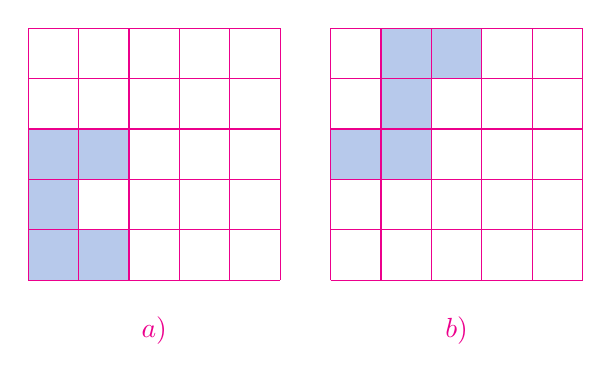
\begin{tikzpicture}[toancuabi,scale=0.64]
			\filldraw [cackithi!40] (0,0) rectangle (1,3);
			\filldraw [cackithi!40] (1,0) rectangle (2,1);
			\filldraw [cackithi!40] (1,2) rectangle (2,3);
			\filldraw [cackithi!40] (6,2) rectangle (8,3);
			\filldraw [cackithi!40] (7,3) rectangle (8,5);
			\filldraw [cackithi!40] (8,4) rectangle (9,5);
			\draw (0,0) grid (5,5);
			\draw (6,0) grid (11,5);
			\draw (2.5, -1) node {$a)$};
			\draw (8.5, -1) node {$b)$};
		\end{tikzpicture}
		\vspace*{-30pt}
	\end{figure}
	\textbf{\color{toancuabi}Bài toán số $\pmb{10}$: (IMSO).}
	\vskip 0.1cm
	Một hình tròn và một tam giác được xếp trên các điểm cắt của lưới ô vuông như hình vẽ sao cho tam giác và hình tròn không cùng nằm trên một hàng hay một cột.
	\vskip 0.1cm
		Hỏi có bao nhiêu cách xếp tam giác và hình tròn vào lưới ô vuông như hình vẽ này. Trên hình vẽ là một ví dụ về cách xếp tam giác và hình tròn.
		\begin{figure}[H]
			\centering
			\vspace*{-10pt}
			\captionsetup{labelformat=empty, justification=centering}
			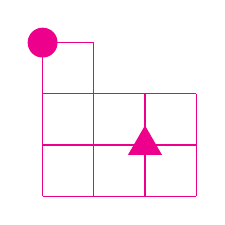
\begin{tikzpicture}[scale= 0.65,toancuabi]
				\draw (0,0) grid (3,2);
				\draw (0,2) grid (1,3);
				\draw[fill = toancuabi] (0,3) circle (8pt);
				\node[fill=white, toancuabi,regular polygon, regular polygon sides=3,inner sep=2.5pt] at (2,1) {};
			\end{tikzpicture}
			\vspace*{-10pt}
		\end{figure}
	\vskip 0.1cm
	\textbf{\color{toancuabi}Phân tích bài toán:} Bài toán này các bạn nhỏ lớp $4,5$ trong câu lạc bộ toán UMC đã làm được theo nhiều cách khác nhau, các bạn quan sát sẽ thấy ngoài hai điểm ở hàng trên cùng thi bên dưới cứ mỗi hình chữ nhật sẽ có $2!\times 2!=4$ cách đặt hình tròn và tam giác (do mỗi cặp đỉnh không kề nhau của $1$ hình chữ nhật sẽ có $2!$ cách đặt hình tròn và tam giác). Sau đây là một số cách giải của các bạn.
	\vskip 0.1cm
	\textit{Lời giải $1$: }(Lê Kỳ Nam, Vĩnh Giang)
	\vskip 0.1cm
	Nếu đường tròn nằm trên hàng đầu tiên (có $2$ vị trí), thì ở mỗi vị trí sẽ có $14 - 4 - 1 = 9$ cách chọn tam giác, tổng số cách chọn là: $9 \times 2 = 18$.
	\vskip 0.1cm
	Nếu đường tròn đi vào phần còn lại của $2$ cột đầu tiên, thì ở mỗi vị trí, số cách chọn tam giác là $14 - 3 - 3 - 1 = 7$, tổng số cách chọn là $6 \times 7 = 42$.
	\vskip 0.1cm
	Nếu đường tròn đi ở $2$ cột cuối cùng, thì ở mỗi vị trí, tam giác sẽ có $14 - 3 - 2 - 1 = 8$ lựa chọn, tổng số cách chọn là $6 \times 8 = 48$.
	\vskip 0.1cm
	Tổng số cách xếp hình tròn và hình tam giác là: $18 + 42 + 48 = 108$.
	\vskip 0.1cm
	Đáp số: $108$
	\vskip 0.1cm
	\textit{Lời giải $2$:} (Nguyễn Gia Tuấn)
	\vskip 0.1cm
	Nếu hình tròn và hình tam giác không được đặt trên hình vuông trên cùng thì có $3 \times 4 \times 2 \times 3 = 72$ cách chọn.
	\vskip 0.1cm
	Nếu một trong các tam giác hoặc hình tròn được đặt trên hình vuông trên cùng thì có $2 \times 3 \times 3 \times 2 = 36$ cách chọn.
	\vskip 0.1cm
	Tổng cộng có $72 + 36 = 108$ cách chọn.
	\vskip 0.1cm
	\textit{Lời giải $3$:} (Nguyễn Trọng Cường).
	\vskip 0.1cm
	Tổng số các cách có thể đặt hình tròn và tam giác vào $2$ điểm bất kỳ của hình là: $14\times13 = 182$ cách
	\vskip 0.1cm
	Nếu hình tròn và tam giác nằm trên cùng $1$ cột, hoặc $1$ hàng, thì $2$ điểm sẽ tạo nên $1$ đoạn thẳng. Ta đếm số đoạn thẳng của hình trên.
	\vskip 0.1cm
	Số đoạn thẳng của hình là :
	\begin{align*}
		&1 + (1+2+3) \times 3 + (1+2+3) \times 2 \\
		&+ (1+2) \times 2 = 37
	\end{align*}
	Hình tròn và tam giác ở $2$ đầu đoạn thẳng, đổi chỗ được cho nhau $\Rightarrow$ có $37 \times 2 = 74$ cách ko thỏa mãn
	\vskip 0.1cm
	Số cách thỏa mãn đề bài là $182 - 74 = 108$ cách.
	\vskip 0.1cm
	\textit{Lời giải $4$:} (Nguyễn Gia Tuấn). -- Dùng phần bù:
	\vskip 0.1cm
	Với lưới ô vuông $3 \times 3$ thì ta có $C(4,2)\times C(4,2)\times 4 = 144$ cách chọn. (Do mỗi hình chữ nhật có $4$ cách đặt tam giác và hình tròn).
	\vskip 0.1cm
	Trong lưới $3 \times 3$ đó, nếu đặt hình tròn hoặc tam giác vào $2$ điểm trên cùng ở bên phải thì có $2 \times 3 \times  3 \times 2 = 36$ cách chọn.
	\vskip 0.1cm
	Vậy ta có $144 - 36 = 108$ cách chọn để xếp hình tròn và hình tam giác.
	\vskip 0.1cm
	Trả lời: $108$ lựa chọn.
\end{multicols}
\newpage
\begingroup
\AddToShipoutPicture*{\put(122,675){
\includegraphics[scale=1]{../tieude.pdf}}}  
\centering
\endgroup
\vspace*{25pt} 
\begin{multicols}{2}
	Cùng với cảnh sát thành phố, thám tử Xuân Phong đã tóm gọn được một băng cướp gồm $50$ tên. Tuy nhiên khi tra hỏi, tên cướp nào cũng muốn làm giảm nhẹ tội lỗi của mình. Qua điều tra, Xuân Phong biết rằng tất cả $50$ tên chưa từng cùng tham gia một vụ cướp, tuy nhiên cứ hai tên bất kỳ trong số chúng đều đã gặp gỡ nhau tại các vụ cướp bóc chung duy nhất đúng một lần. Khi khai nhận, tất cả các tên cướp đều trả lời rằng, chúng chỉ mới đi trộm cắp cướp giật và số vụ cướp mà mỗi tên tham gia đều ít hơn $8$ vụ. Xuân Phong nghe lời khai của chúng đã xác định được ngay có ít nhất một tên cướp đã nói dối. Em có biết vì sao Xuân Phong lại kết luận được như vậy hay không?
	%	Giả sử tất cả các tên cướp đều khai thật. Ta chọn một tên cướp bất kỳ, gọi tên là $A$. Tên này tham gia không quá $7$ vụ cướp, hơn nữa $49$ tên còn lại đều chỉ tham gia đúng duy nhất một vụ cướp chung với $A$. Theo nguyên lý Dirichlet, phải có một vụ cướp (đặt tên là $T$) mà có không ít hơn $7$ tên trong số $49$ tên còn lại tham gia. Cùng với $A$, sẽ có không ít hơn $8$ tên cướp tham gia vụ cướp $T$ này. Vì $50$ tên cướp không cùng tham gia một vụ, nên phải có một tên không tham gia vụ $T$. Ta gọi đó là tên cướp $B$. 
	%	\vskip 0.1cm
	%	Ta sẽ chỉ ra $B$ tham gia ít nhất $8$ vụ cướp. Thật vậy, theo kết luận điều tra $B$ có tham gia các vụ cướp cùng với mỗi tên trong số tất cả các tên tham gia vụ $T$, hơn nữa tất cả các vụ cướp đó là khác nhau.  Nếu không, sẽ có hai vụ cướp trùng nhau. Điều đó có nghĩa là có hai tên cướp (đặt tên là $X$ và $Y$) sao cho $B,X,Y$ cùng tham gia một vụ $S$ ($S$ khác với $T$); hơn nữa $X,Y$ cũng đã tham gia cả vụ cướp $T$. Suy ra $X,Y$ cùng tham gia cả $2$ vụ cướp khác nhau là $S$ và $T$. Điều này mâu thuẫn với kết luận điều tra.
	%	\vskip 0.1cm
	%	Mâu thuẫn trên chỉ ra phải có một tên cướp khai gian dối. Điều này có nghĩa ít nhất có một tên đã tham gia không ít hơn $8$ vụ cướp.
\end{multicols}
\begin{figure}[H]
	\centering
	\vspace*{-15pt}
	\captionsetup{labelformat= empty, justification=centering}
	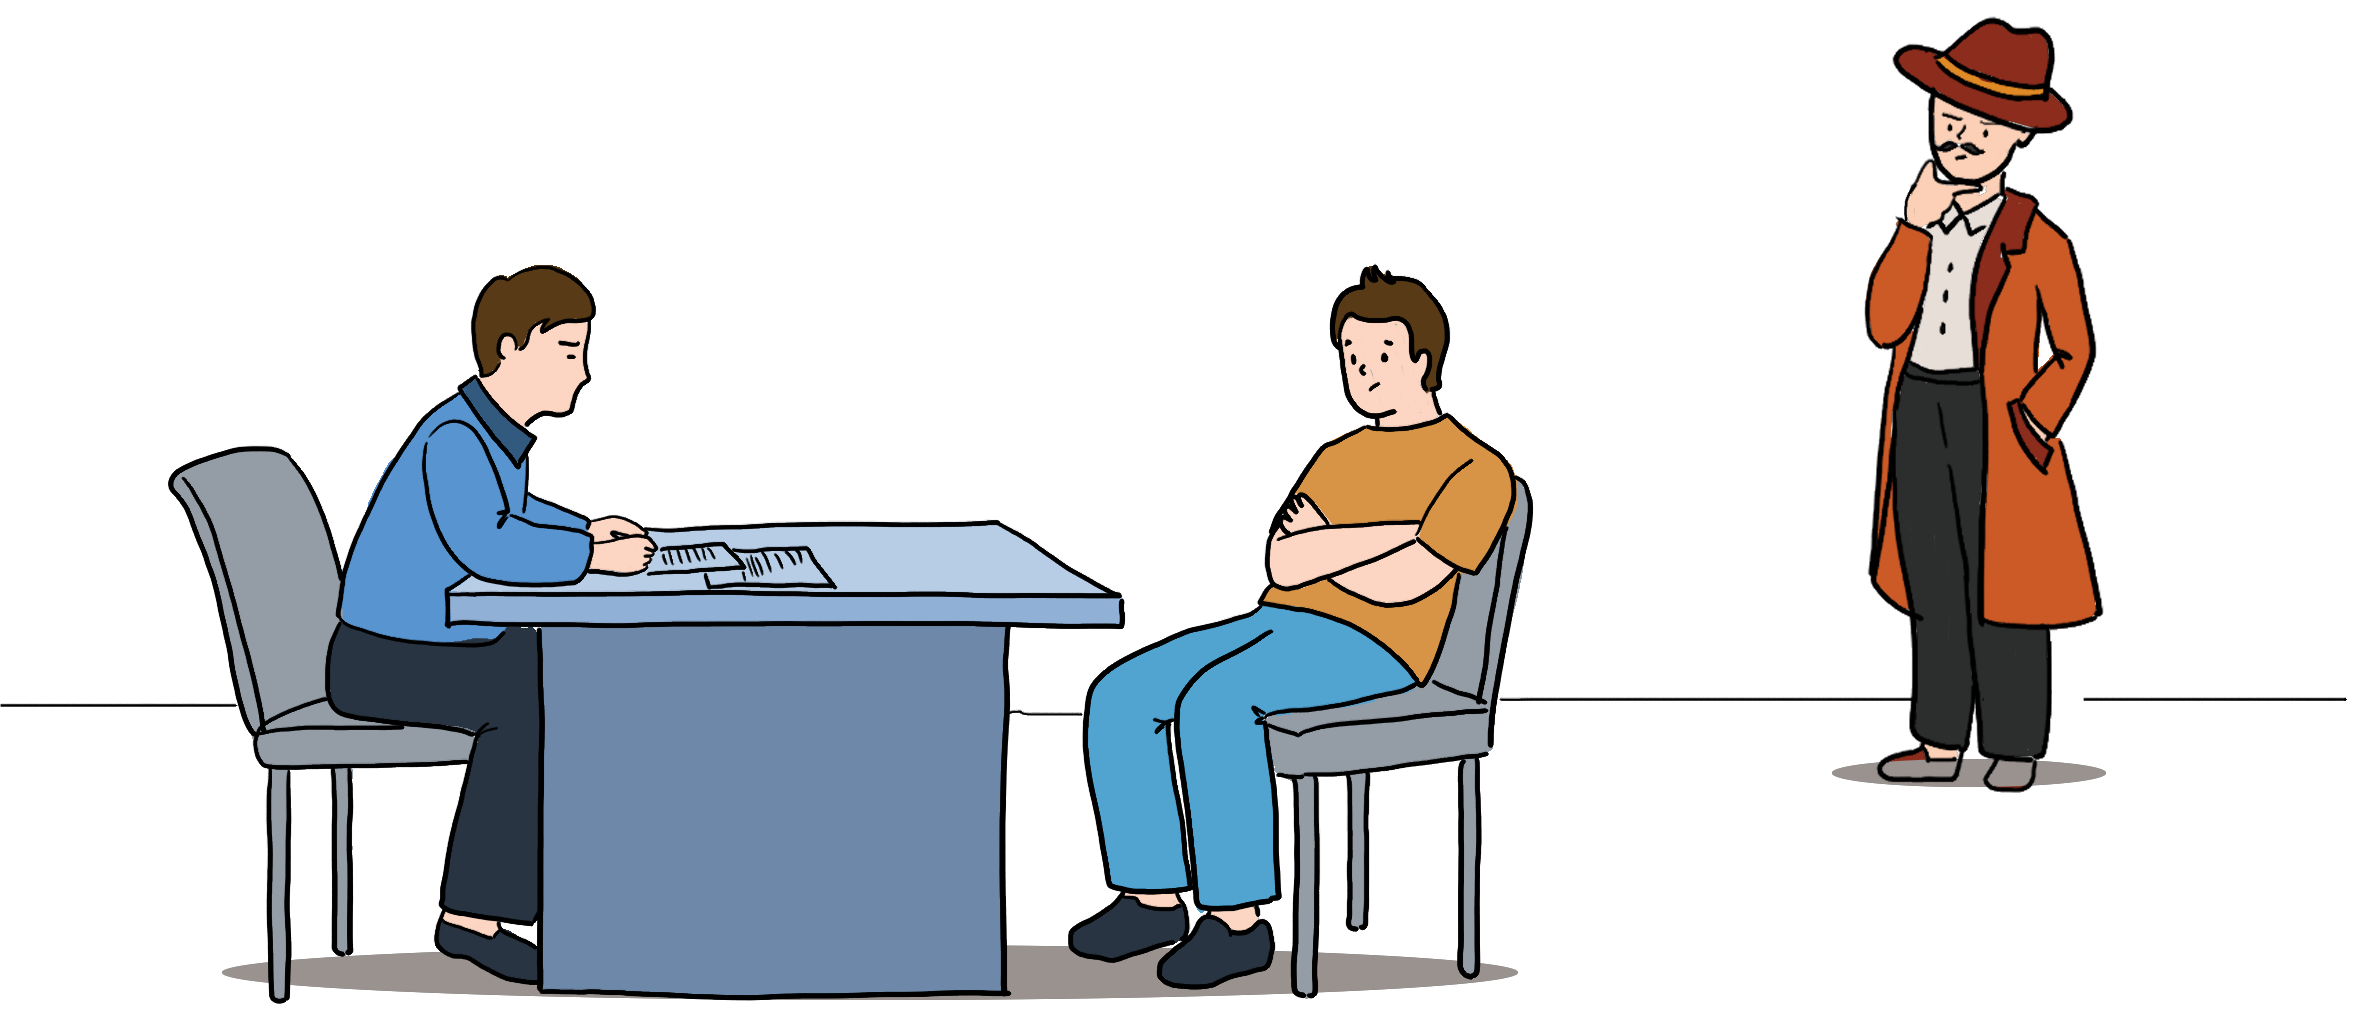
\includegraphics[width=0.85\linewidth]{xp}
	\vspace*{-10pt}
\end{figure}
\vspace*{-10pt}
{\color{toancuabi}\rule{1\linewidth}{0.1pt}}
\begingroup
\AddToShipoutPicture*{\put(115,315){
\includegraphics[scale=1]{../tieude11.pdf}}} 
\centering
\endgroup
\vspace*{45pt}

\begin{multicols}{2}
	$\pmb{1.}$ Ở nhà một mình, bé Hoa rót ra một cốc sữa đầy và uống hết một nửa. Sau đó Hoa rót thêm nước ép táo vào cho đầy cốc, rồi lại uống hết một nửa. Cuối cùng, bé lại rót thêm nước ép táo vào đầy cốc rồi uống hết sạch cả cốc. Hỏi bé Hoa đã uống thứ gì nhiều hơn: sữa hay nước ép táo?
	\begin{figure}[H]
		\centering
		\vspace*{-5pt}
		\captionsetup{labelformat= empty, justification=centering}
		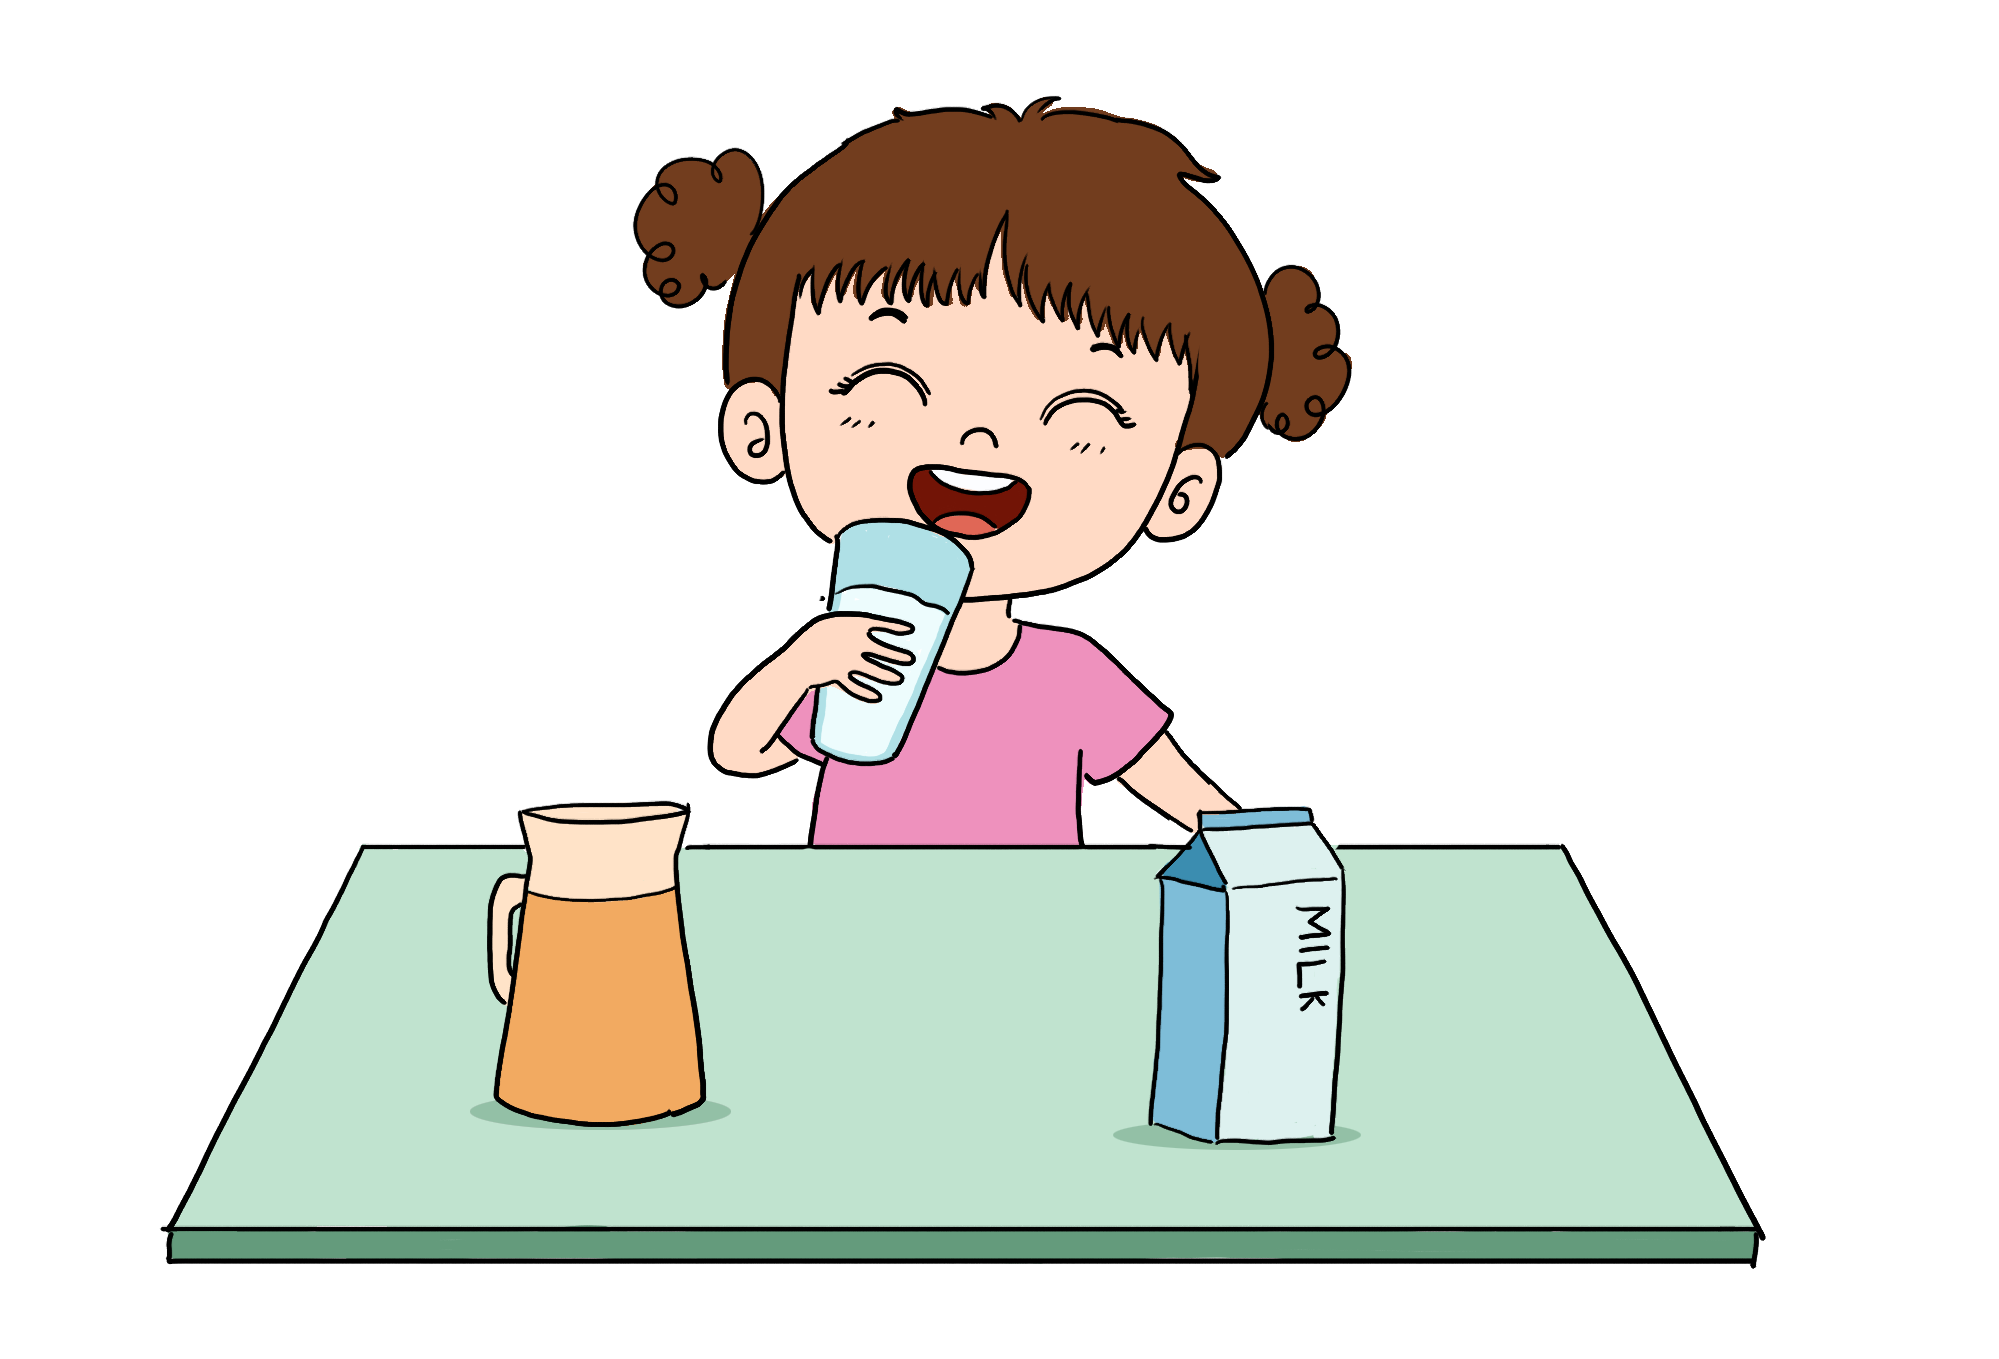
\includegraphics[width=0.9\linewidth]{Pi6_bai1}
		\vspace*{-5pt}
	\end{figure}
	$\pmb{2.}$ Dê con và Sói cùng thi xem ai chạy từ nhà tới bờ suối và quay ngược lại nhanh hơn. Biết rằng khoảng cách từ nhà tới bờ suối là $100$ bước nhảy của Dê con. Một bước nhảy của Sói dài gấp $3$ lần một bước nhảy của Dê con. Tuy nhiên trong khoảng thời gian Sói nhảy được một bước thì Dê con lại nhảy được $3$ bước. Hỏi ai sẽ chiến thắng?
	\begin{figure}[H]
		\centering
		\vspace*{-5pt}
		\captionsetup{labelformat= empty, justification=centering}
		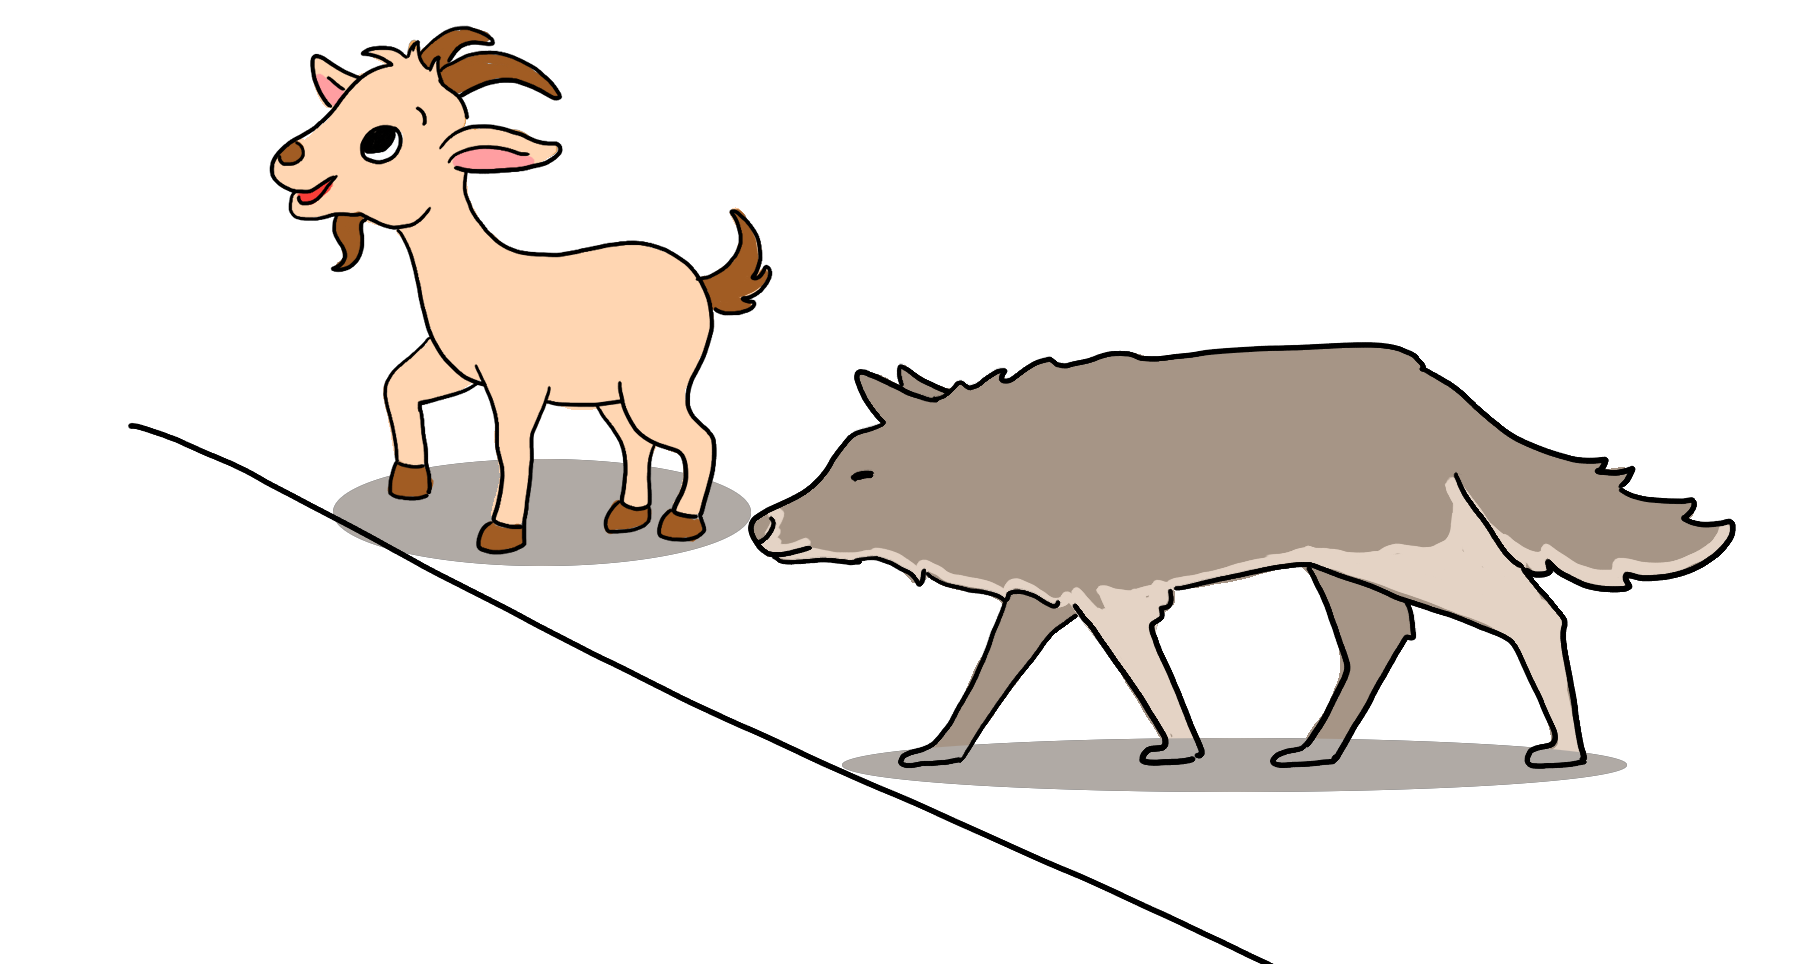
\includegraphics[width=0.95\linewidth]{Pi6_bai2}
		\vspace*{-5pt}
	\end{figure}
	$\pmb{3.}$ 	Có tất cả $25$ chú chim cúc cu và gà trống cùng tham gia một cuộc thi hùng biện giữa các loài vật. Trong số $15$ chú chim bất kỳ luôn có ít nhất một chú gà trống, và trong số $12$ chú chim bất kỳ luôn có ít nhất một chú chim cúc cu. Hỏi trong cuộc thi đó có bao nhiêu chú gà trống và bao nhiêu chú chim cúc cu tham gia?
	\begin{figure}[H]
		\centering
		\vspace*{-5pt}
		\captionsetup{labelformat= empty, justification=centering}
		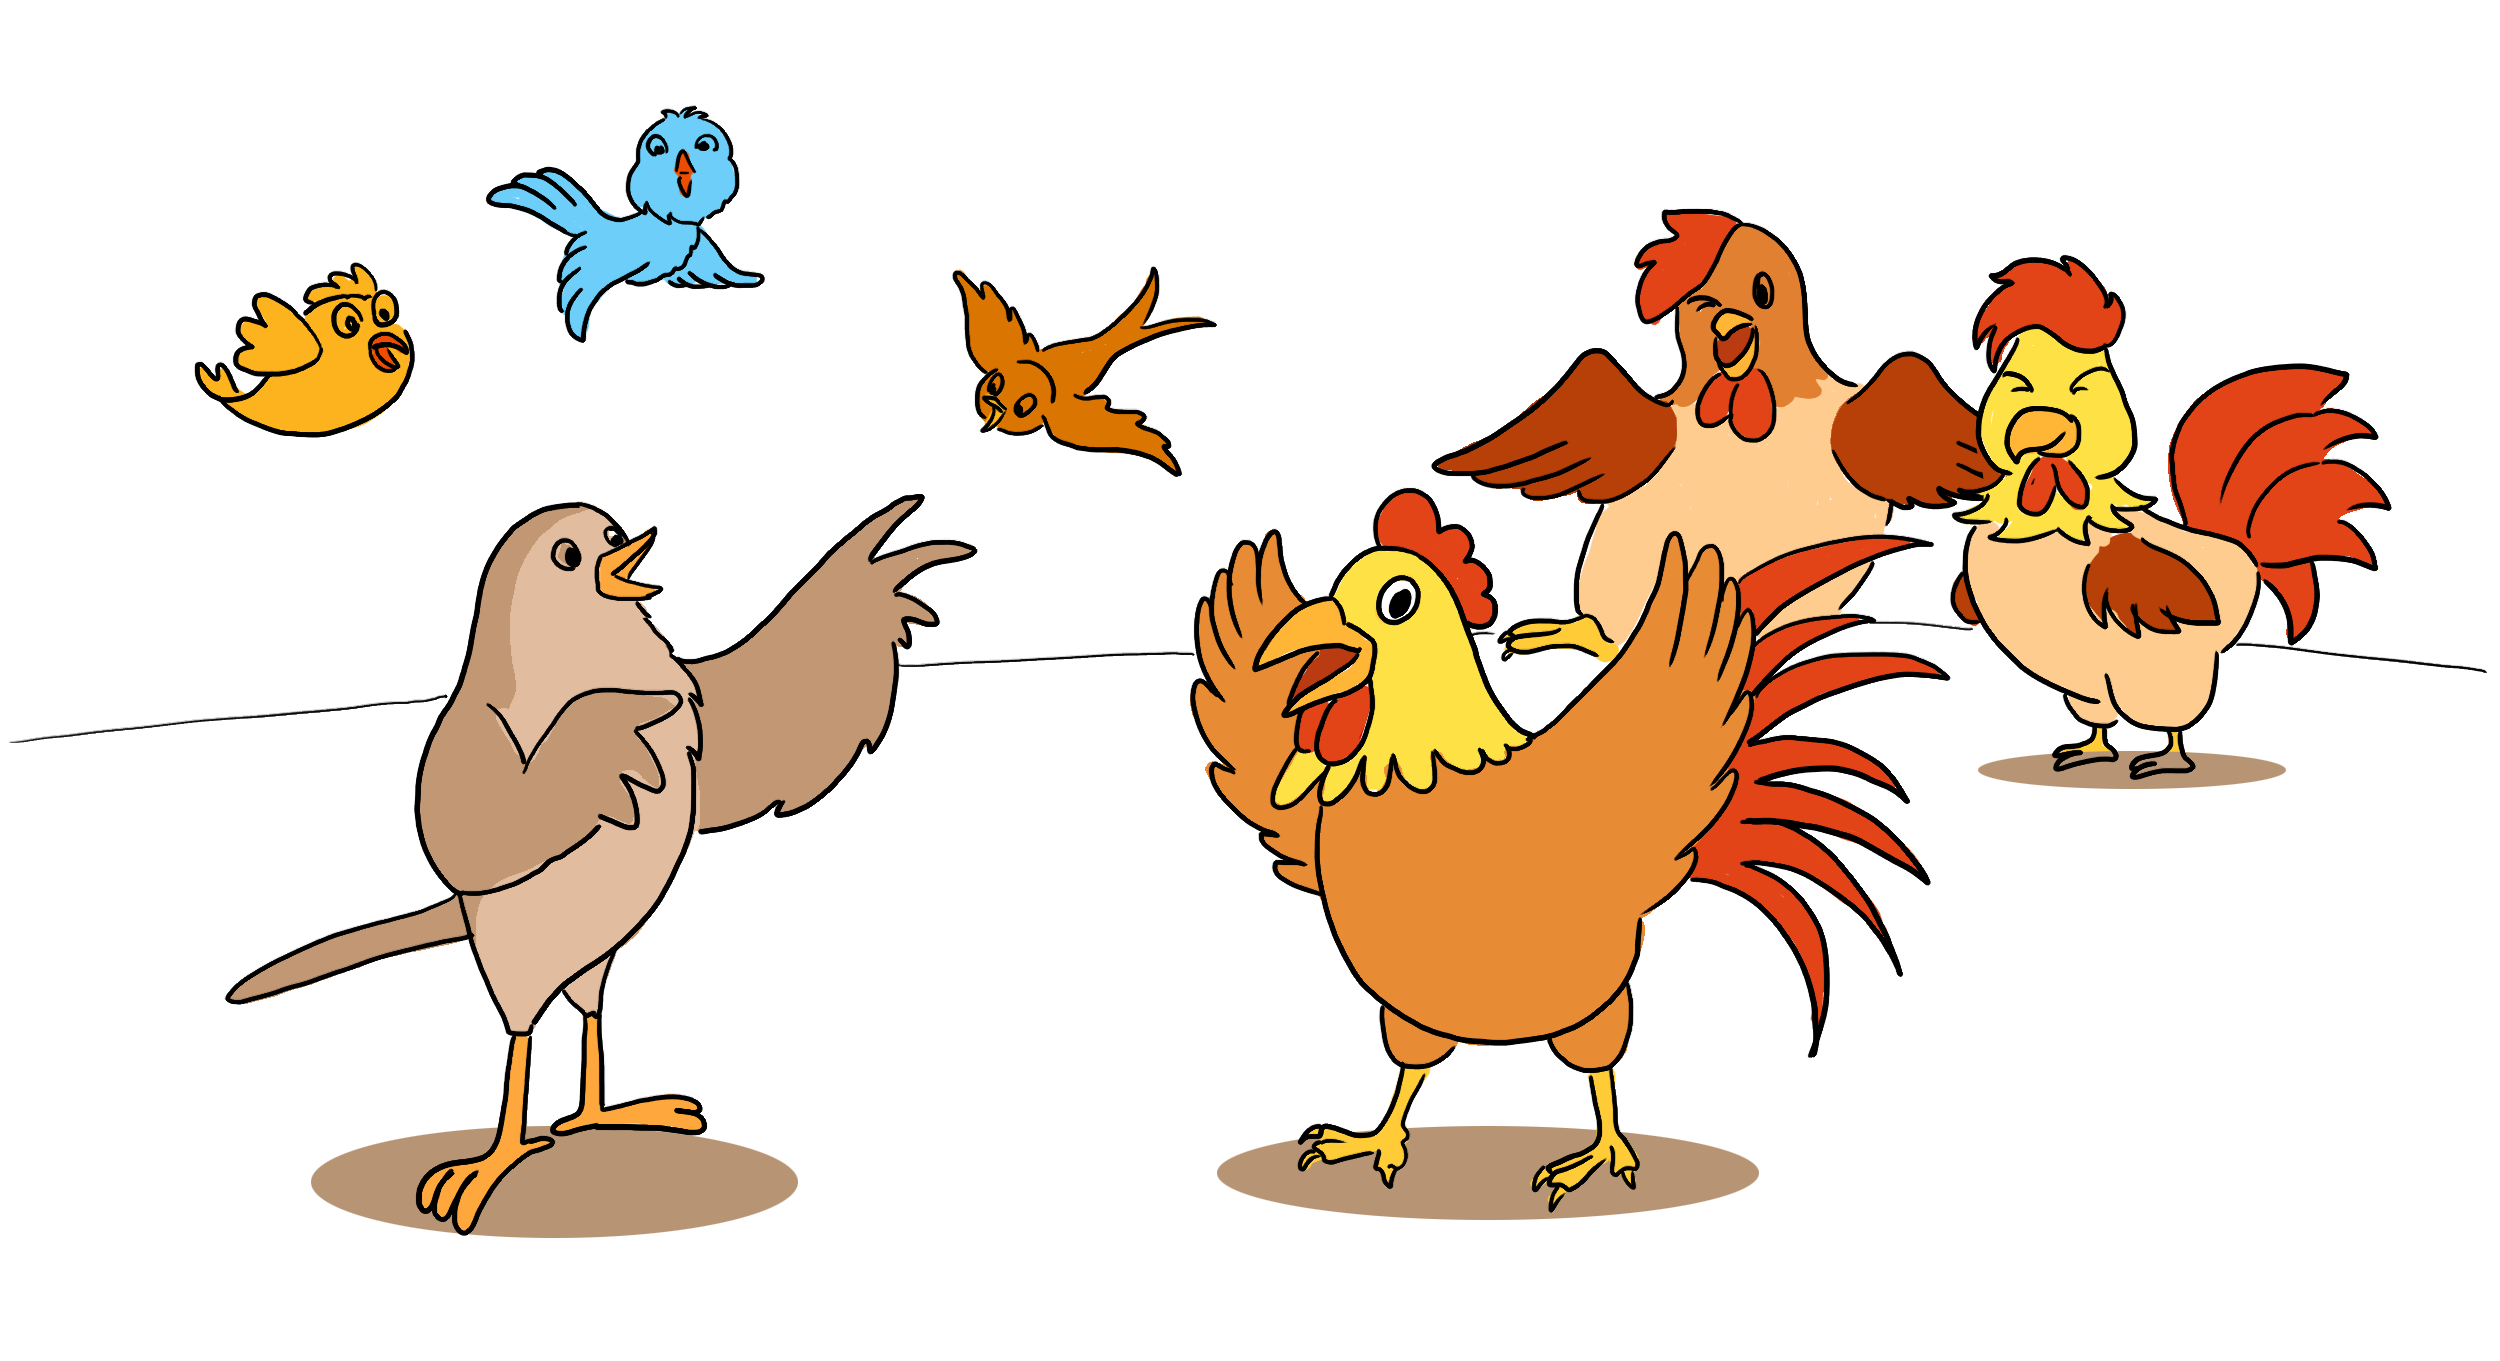
\includegraphics[width=1\linewidth]{Pi6_bai3}
		\vspace*{-10pt}
	\end{figure}
	$\pmb{4.}$ Người ta trồng trong công viên hai loài cây gồm phượng vĩ và sấu. Trong đó phượng vĩ chiếm $60\%$ tổng số hai loài. Vào mùa xuân cây sấu được trồng thêm trong công viên, do đó cây phượng vĩ chỉ còn chiếm $20\%$ tổng số cây. Sang mùa thu người ta lại trồng thêm  phượng vĩ, vì thế cây phượng vĩ lại chiếm $60\%$ tổng số cây hai loài. Hỏi sau hai lần trồng thì số cây trong công viên tăng lên bao nhiêu lần?
	\begin{figure}[H]
		\centering
		\vspace*{-5pt}
		\captionsetup{labelformat= empty, justification=centering}
		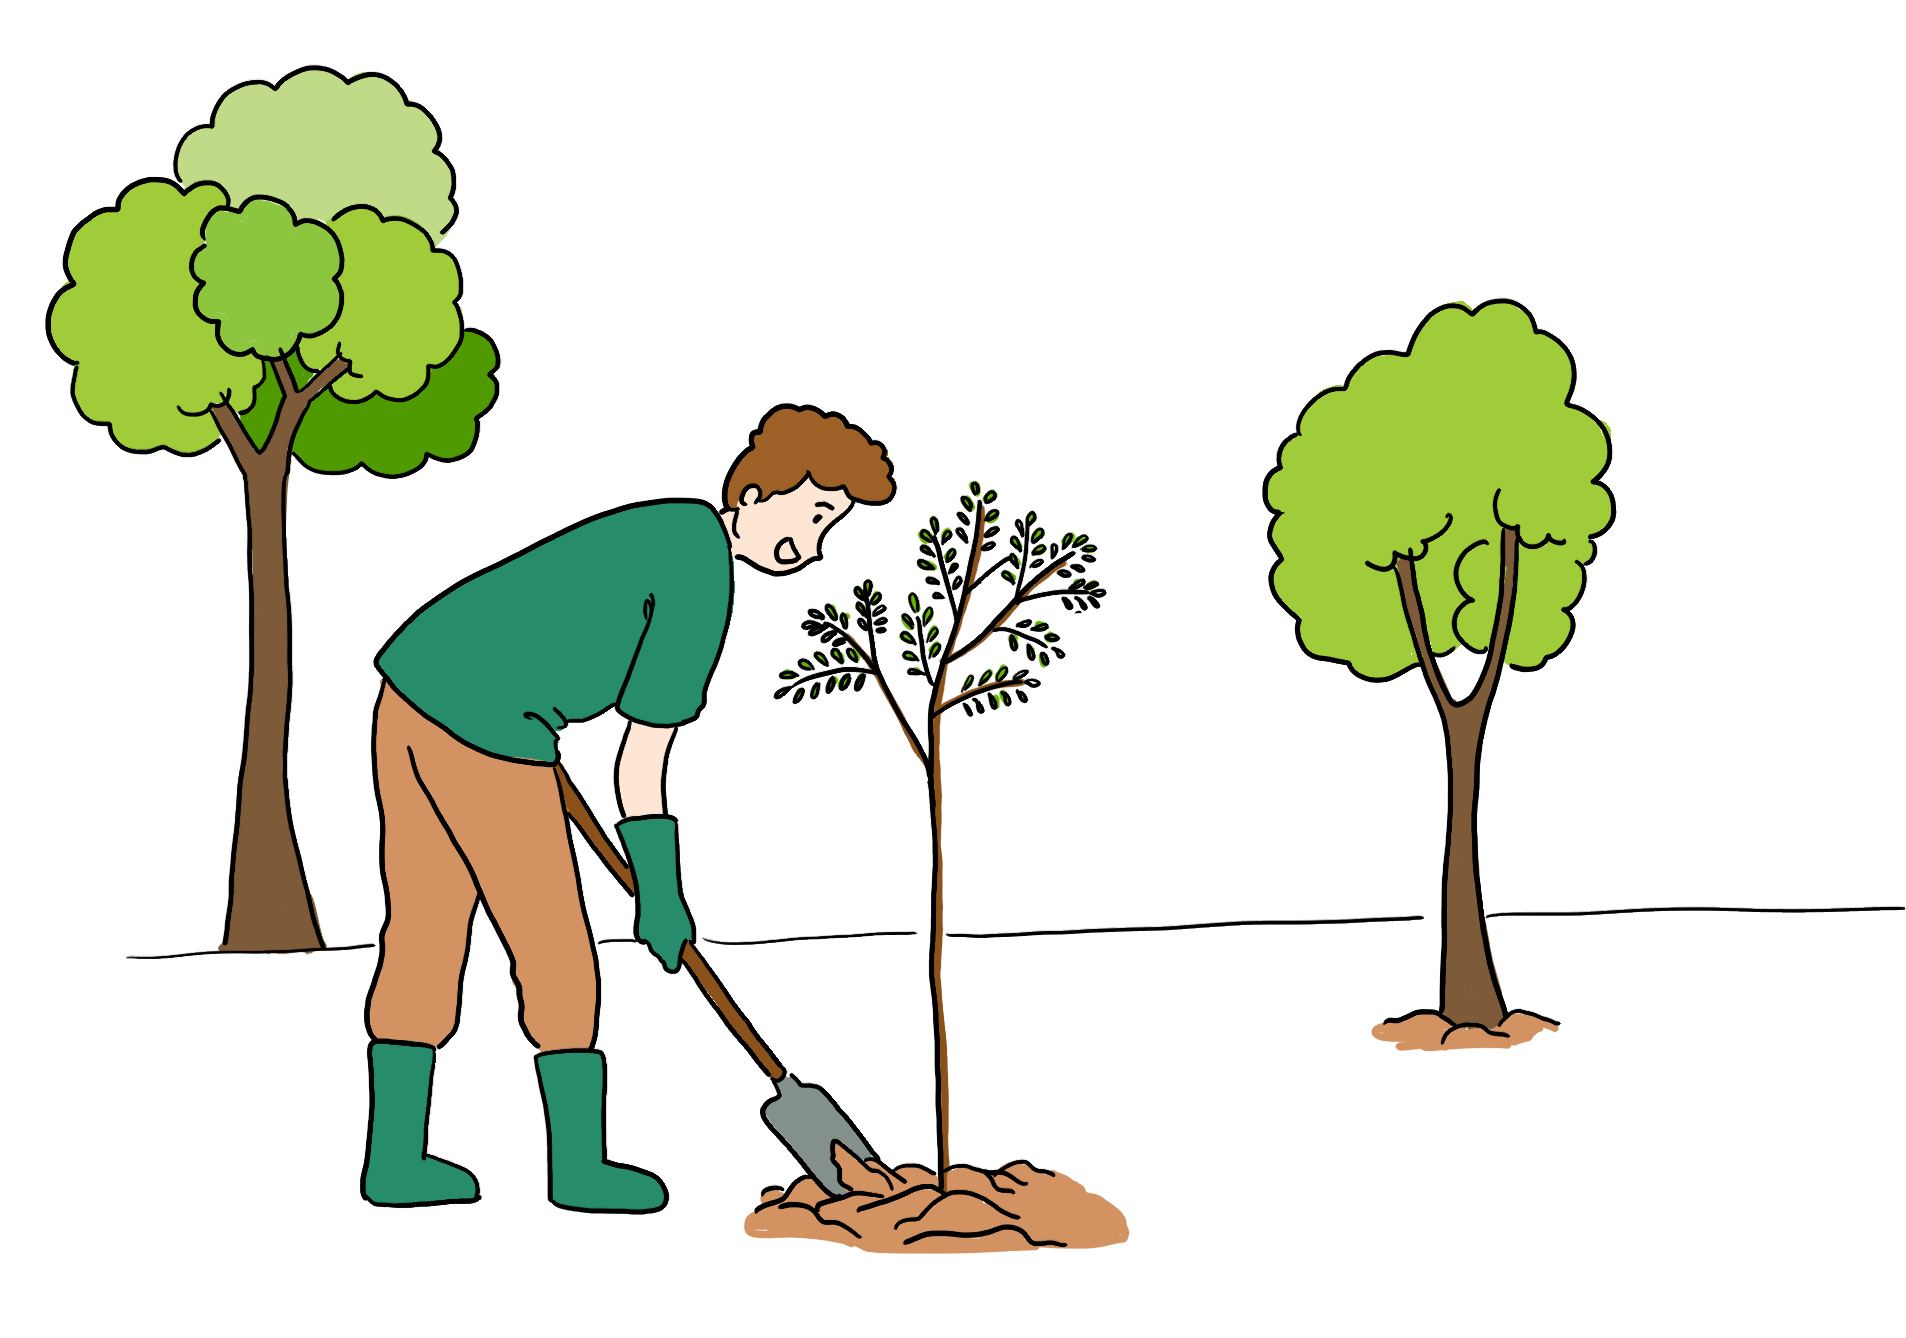
\includegraphics[width=1\linewidth]{Pi6_bai4}
		\vspace*{-10pt}
	\end{figure}
	$\pmb{5.}$ Alibaba đột nhập vào một hang động, trong đó có $100$ chiếc bao vải đựng đầy những đồng tiền. Một chiếc bao vải trong số đó chỉ đựng toàn đồng tiền giả. Khối lượng của một đồng tiền thật là $10$ gram, trong khi khối lượng của một đồng tiền giả là $9$ gram. Hỏi Alibaba làm thế nào để chỉ cân một lần duy nhất (bằng một cái cân chính xác có hiển thị số) tìm ra được bao vải chứa các đồng tiền giả?
	\begin{figure}[H]
		\centering
		\vspace*{-5pt}
		\captionsetup{labelformat= empty, justification=centering}
		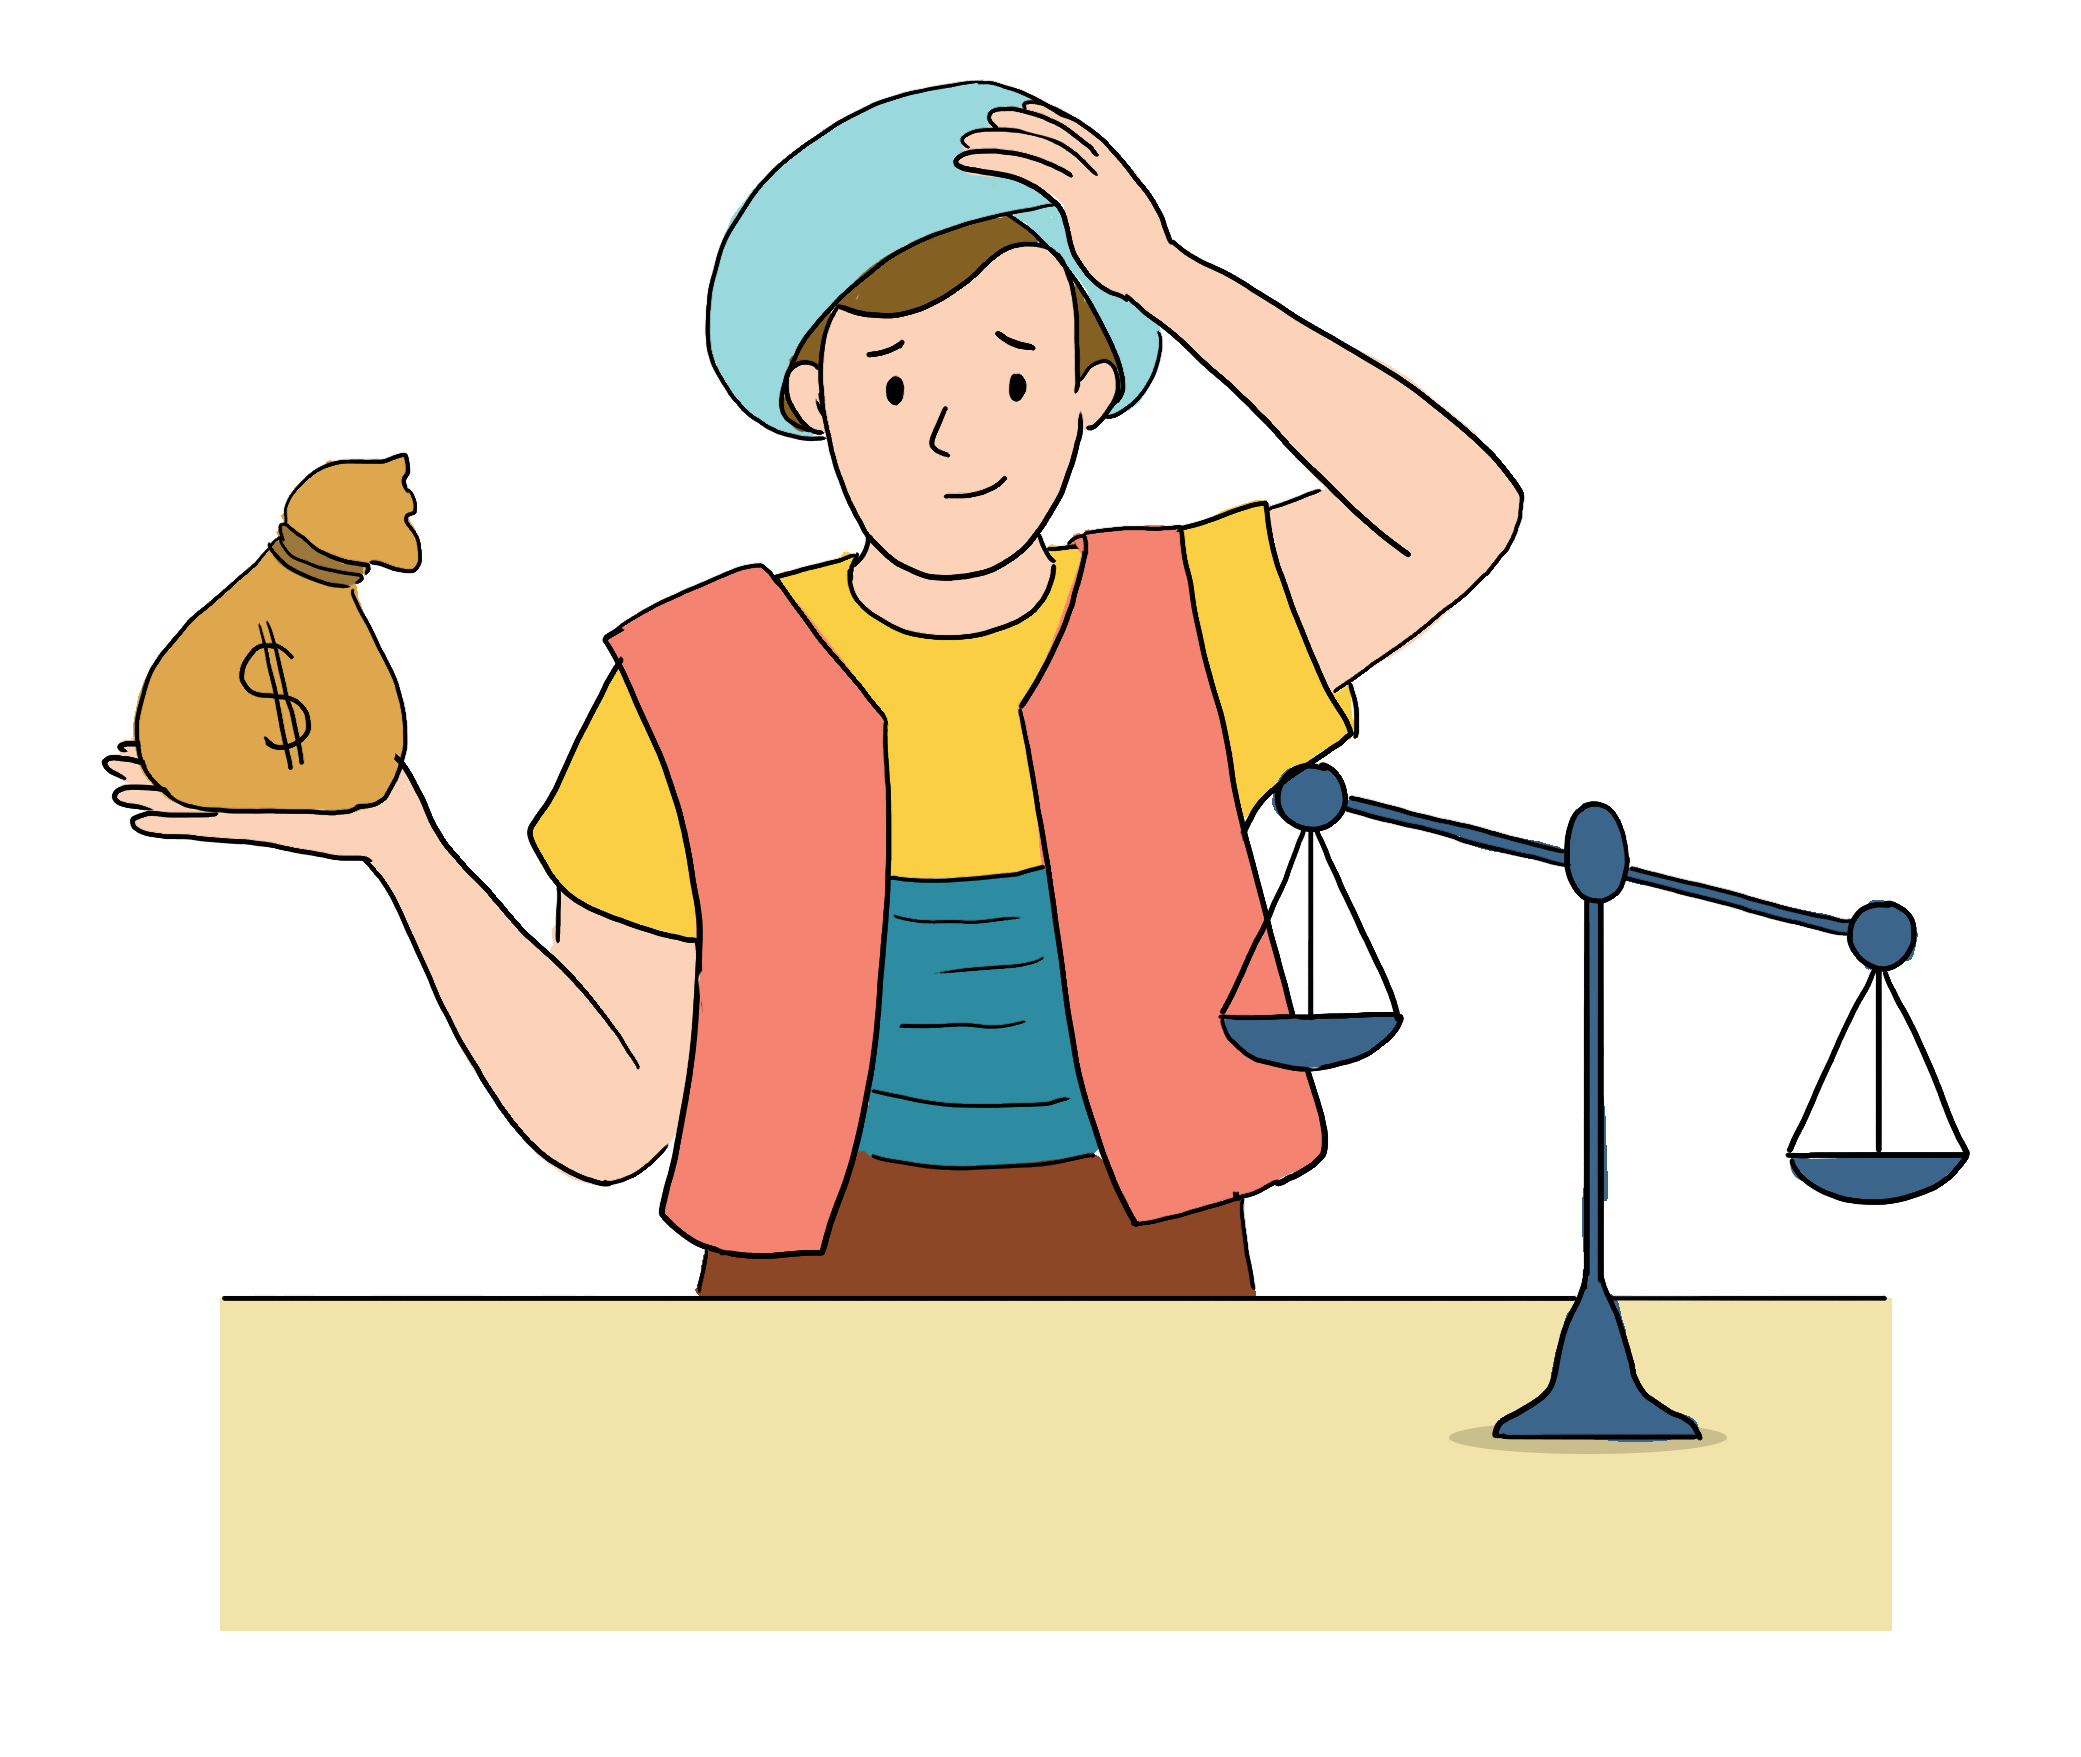
\includegraphics[width=1\linewidth]{Pi6_bai5}
		\vspace*{-10pt}
	\end{figure}
	$\pmb{6.}$ 	Trên một bàn cờ $8\times8$ người ta xếp một số lớn nhất có thể các quân Tượng sao cho không có hai quân Tượng nào ``ăn" lẫn nhau. Em hãy chứng minh rằng số các cách xếp khác nhau như vậy là một số chính phương (tức là bình phương của một số tự nhiên).
	\begin{figure}[H]
		\centering
		\vspace*{-5pt}
		\captionsetup{labelformat= empty, justification=centering}
		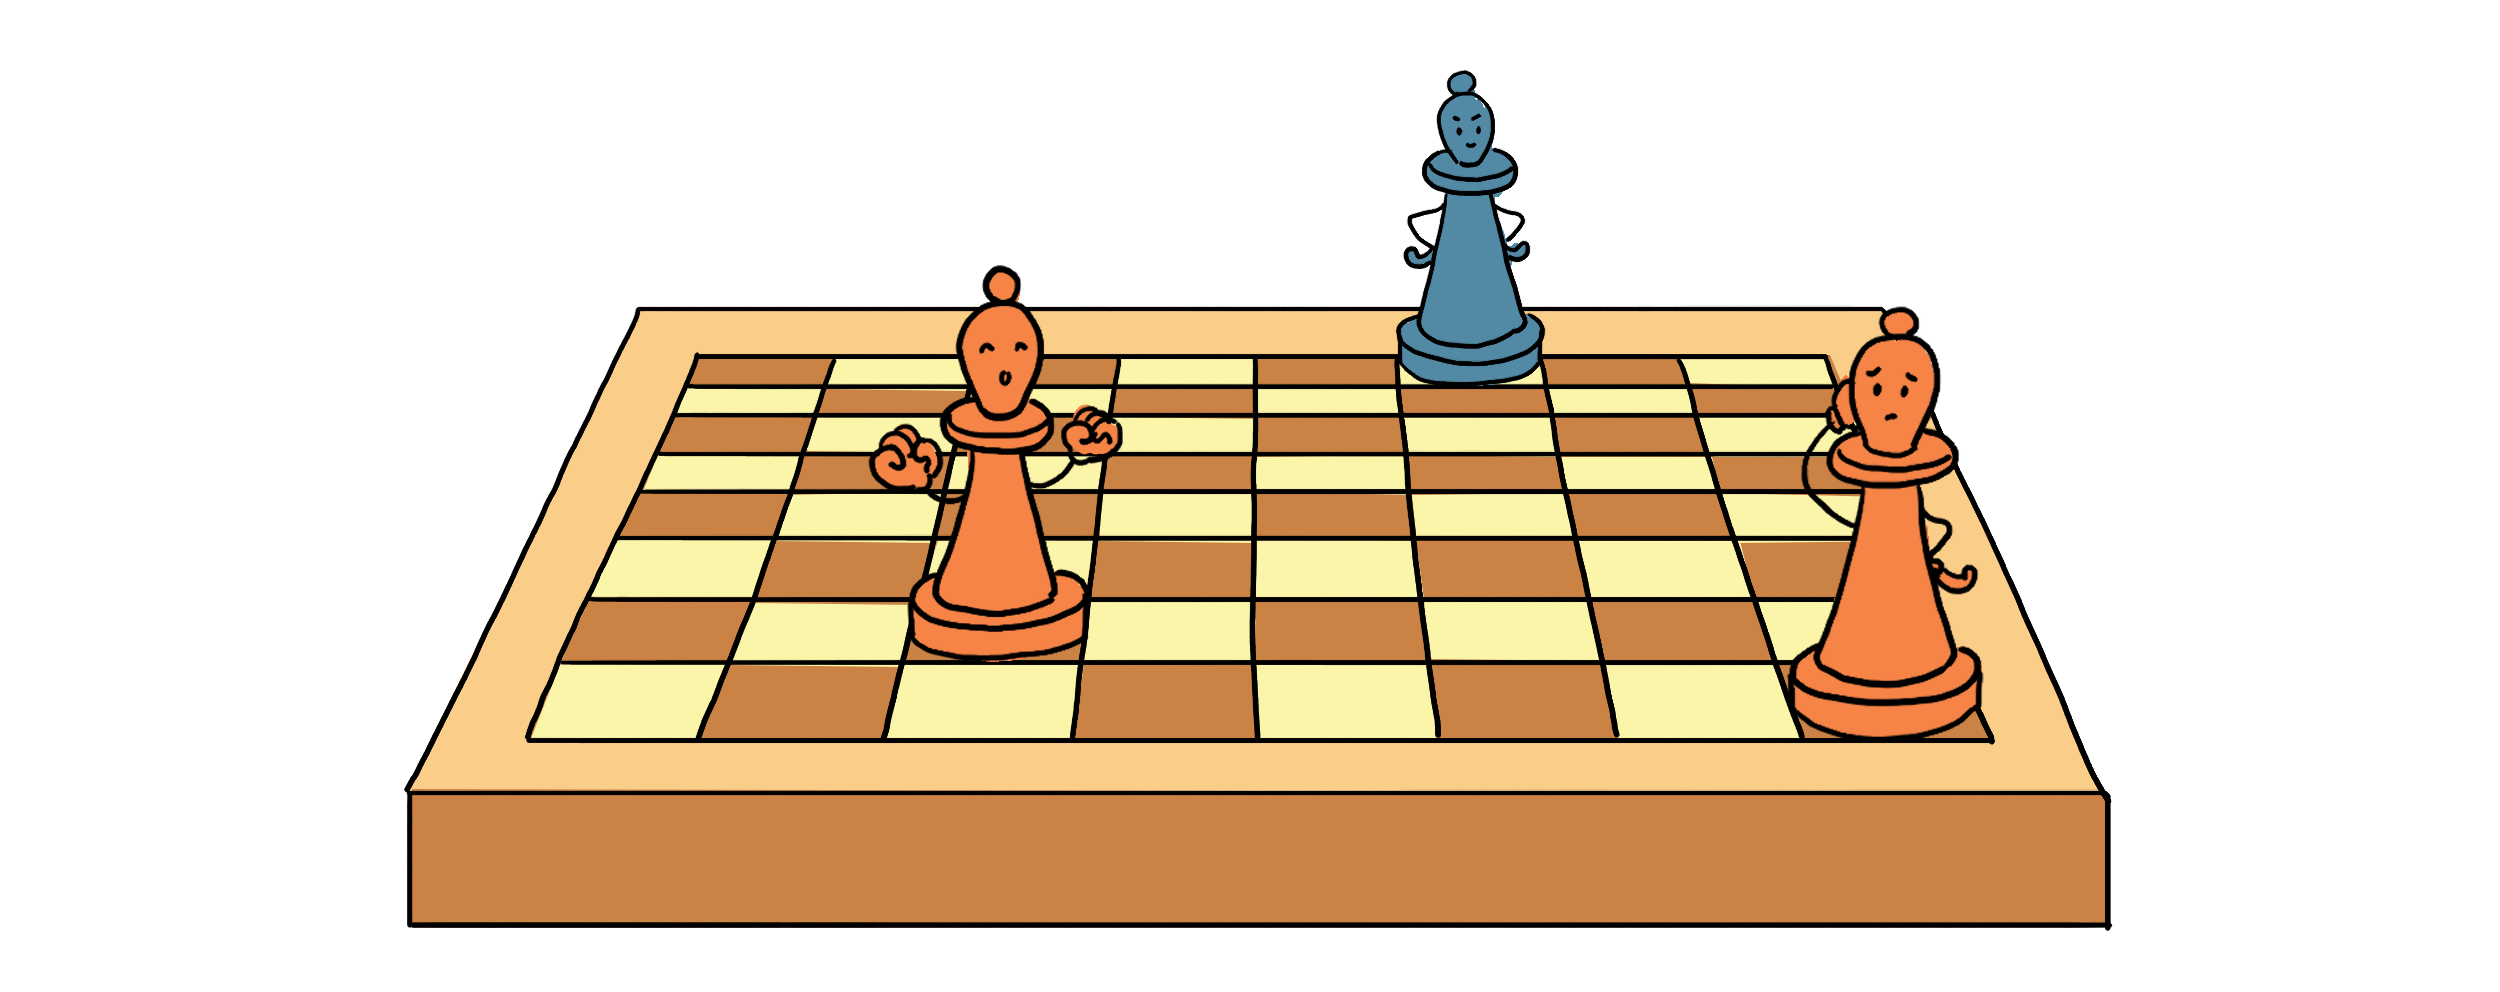
\includegraphics[width=1\linewidth]{Pi6_bai6}
		\vspace*{-5pt}
	\end{figure}
\end{multicols}
\newpage
\begingroup
\AddToShipoutPicture*{\put(112,645){
\includegraphics[scale=1]{../tieude2.pdf}}} 
\centering
\endgroup
\vspace*{55pt}

\begin{multicols}{2}
	$\pmb{1.}$	Bạn Công đã trả $24$ nghìn đồng để mua được $1$ cuốn vở, $2$ chiếc bút chì và $1$ cái tẩy. Bạn Nam thì trả tận $54$ nghìn đồng để mua được $2$ cuốn vở, $3$ chiếc bút chì và $3$ cái tẩy. Hỏi bạn An đã trả bao nhiêu tiền để mua được $2$ cuốn vở, $5$ chiếc bút chì và $1$ cái tẩy?
	\begin{figure}[H]
		\centering
		\vspace*{-5pt}
		\captionsetup{labelformat= empty, justification=centering}
		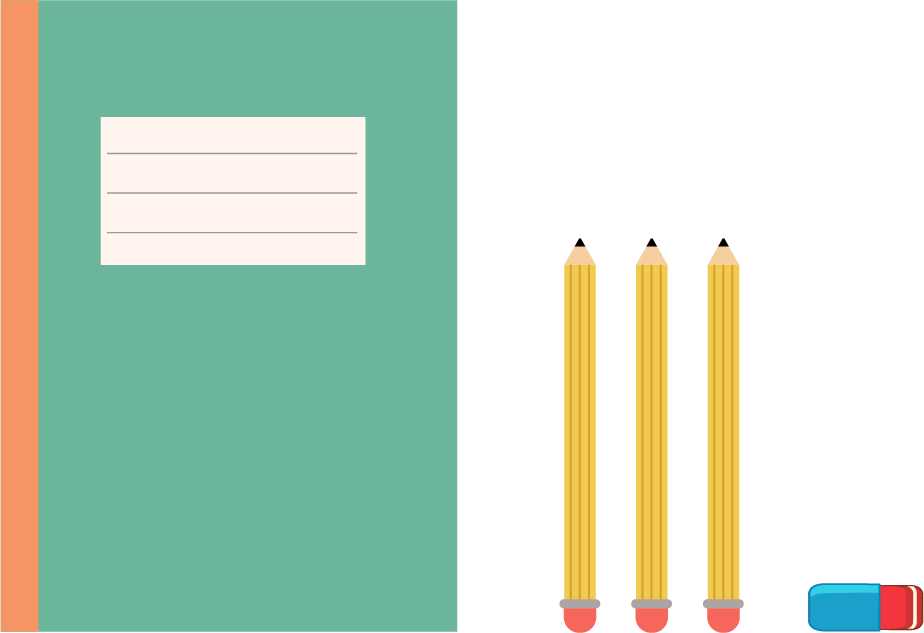
\includegraphics[width=1\linewidth]{Pi3_bai1}
		\vspace*{-10pt}
	\end{figure}
	\textit{Lời giải.} 	Cả $3$ bạn Công, Nam và An đã mua $5$ cuốn vở, $10$ chiếc bút chì và $5$ cái tẩy, bằng đúng $5$ lần số lượng mà Công đã mua. Vì thế $3$ bạn đã trả số tiền là 
	\begin{align*}
		24\times 5=120 \text{(nghìn đồng).} 
	\end{align*}
	Công và Nam đã trả $78$ nghìn đồng. Suy ra An đã trả 
	\begin{align*}
		120-78 = 42 \text{(nghìn đồng).}	
	\end{align*}
	 $\pmb{2.}$ Bác Tuyết mang sữa đựng đầy trong hai chiếc thùng ra chợ bán. Lượng sữa trong thùng to nhiều gấp $3$ lần lượng sữa trong chiếc thùng nhỏ. Khi trong chiếc thùng nhỏ còn có $15$ lít sữa, còn thùng to còn $35$ lít sữa, bác Tuyết đổ dồn một lượng sữa từ thùng to cho đầy chiếc thùng nhỏ. Khi đó trong chiếc thùng to lượng sữa còn lại  đầy tới một nửa thùng. Hỏi bác Tuyết đã đổ bao nhiêu sữa từ thùng to sang thùng nhỏ, và dung tích của mỗi thùng là bao nhiêu?
	 \begin{figure}[H]
	 	\centering
	 	\vspace*{5pt}
	 	\captionsetup{labelformat= empty, justification=centering}
	 	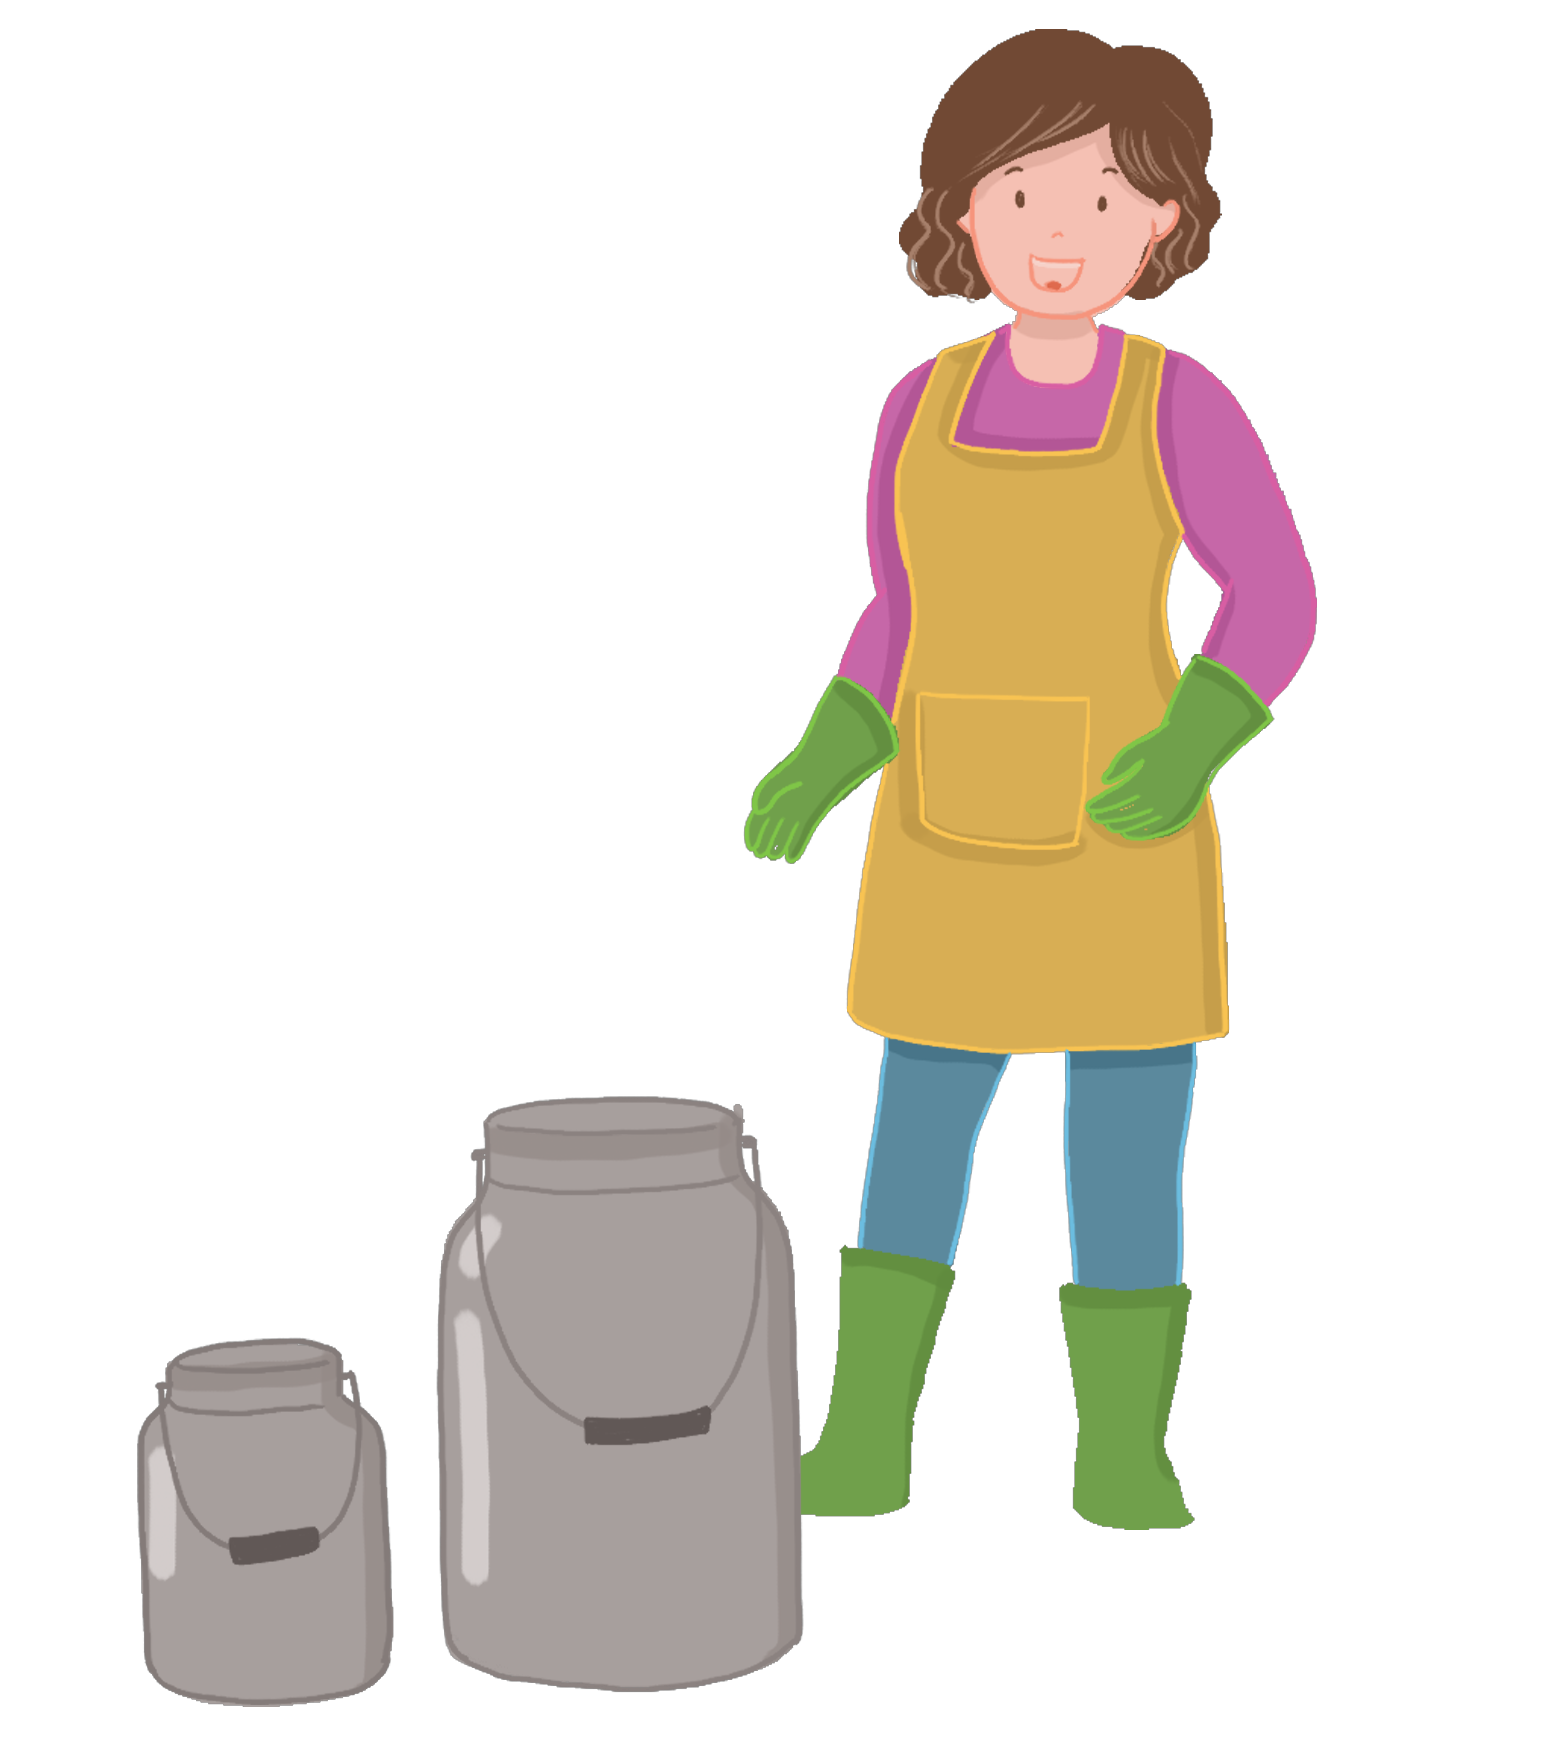
\includegraphics[width=0.75\linewidth]{Pi3_bai2}
	 	\vspace*{-5pt}
	 \end{figure}
	\textit{Lời giải}. Các em nhận thấy, sau khi đổ dồn sữa, số sữa còn lại trong thùng to sẽ gấp rưỡi số sữa trong thùng nhỏ. Gọi số sữa đã đổ dồn sang thùng nhỏ là $a$ ( lít) thì ta có 
	\begin{align*}
		1{.}5\times (15+a)=35-a.
	\end{align*}
	Từ đây suy ra $a =5$. Do đó dung tích của thùng bé là $20$ lít và thùng to là $60$ lít.
	\vskip 0.1cm
	Cách giải khác. Lượng sữa bác Tuyết có lúc đổ từ thùng to thùng nhỏ là $50$ và bằng $2{.}5$ lần dung tích thùng nhỏ. Vậy dung tích thùng nhỏ là 
	\begin{align*}
		50: 2{.}5  = 20 \text{(lít).} 
	\end{align*}
	Số sữa được đổ từ thùng to sang thùng nhỏ là: 
	\begin{align*}
		25-20=5 \text{(lít).} 
	\end{align*}
	Và dung tích thùng to là 
	\begin{align*}
		3 \times 20=60 \text{(lít).}
	\end{align*}
	$\pmb{3.}$ Một tấn hoa quả được chở tới siêu thị: táo được đóng theo các thùng gỗ  $48$ kg/thùng, lê được đóng trong các thùng gỗ $20$ kg/thùng, mận đựng trong hộp giấy theo $14$ kg/hộp còn nho đựng trong các hộp giấy theo $10$ kg/hộp. Biết rằng số kg táo được chở tới nhiều gấp đôi số kg lê, còn số kg mận và nho là bằng nhau, hỏi số lượng mỗi loại hoa quả đã được vận chuyển tới cửa hàng là bao nhiêu?
	\begin{figure}[H]
		\centering
		\vspace*{-5pt}
		\captionsetup{labelformat= empty, justification=centering}
		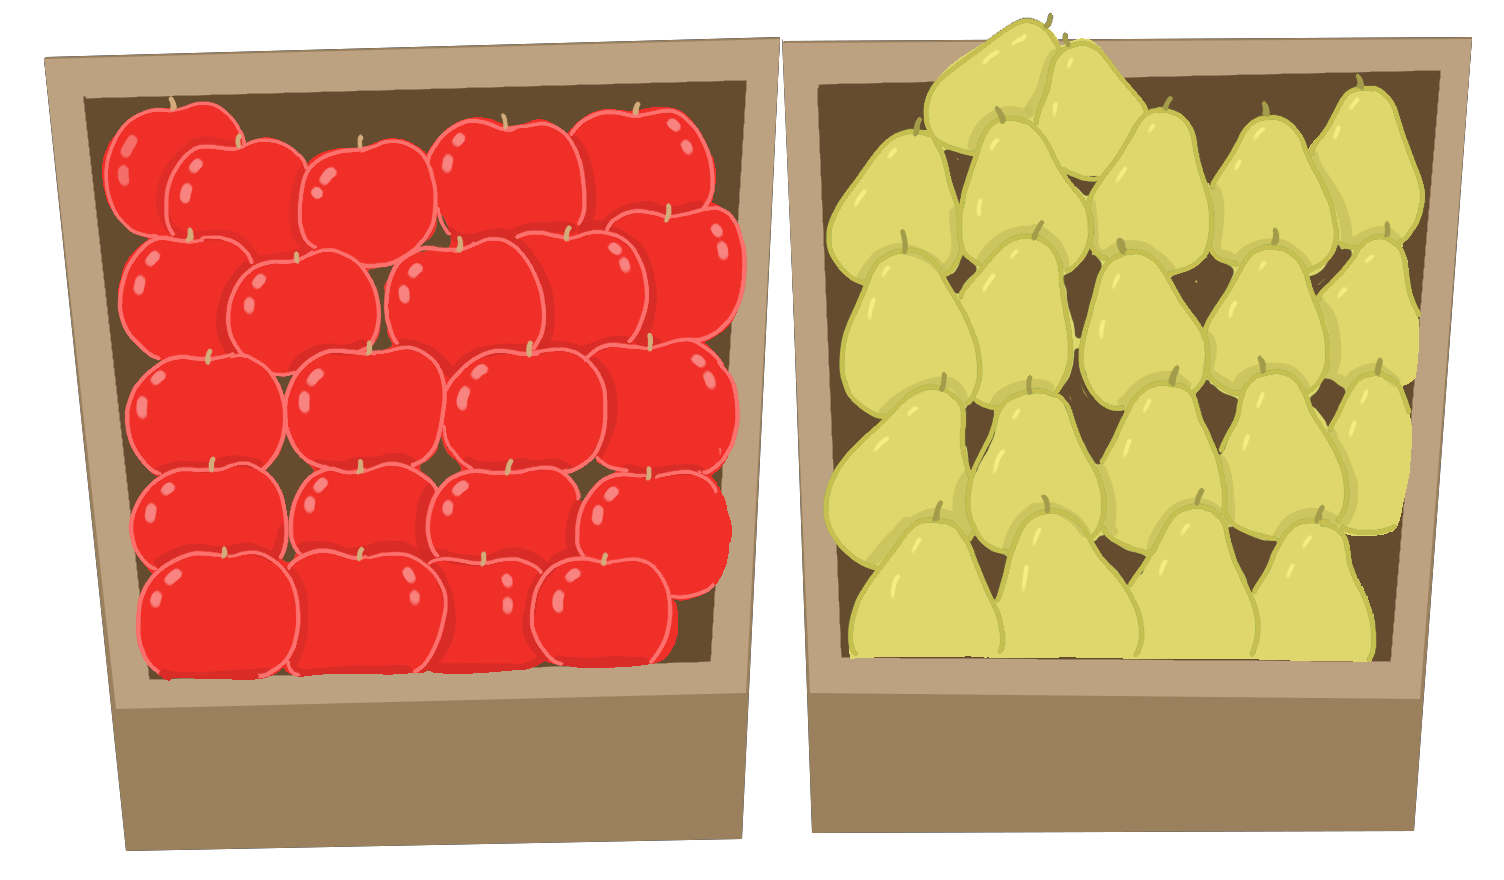
\includegraphics[width=1\linewidth]{Pi3_bai3}
		\vspace*{-15pt}
	\end{figure}
	\textit{Lời giải.} Gọi số thùng táo là $a$, số hộp mận là $b$. Suy ra số thùng lê là 
	\begin{align*}
		\dfrac{48 \times a}{40} = \dfrac{6 \times a}{5}.
	\end{align*}
	Số hộp nho là
	\begin{align*}
		\dfrac{14 \times b}{10} = \dfrac{7 \times b}{5}.
	\end{align*}
	Theo đề bài ta có tổng số kg các loại quả là: 
	\begin{align*}
		48a+24a+14b+14b =1000. 
	\end{align*}
	Có nghĩa là
	\begin{align*}
		72a+28b=1000.
	\end{align*}
	Chia cả hai vế cho $4$, ta nhận được 
	\begin{align*}
		18a+7b=250.
	\end{align*}
	Vì $\dfrac{6 \times a}{5}$ là số nguyên, suy ra $a$ chia hết cho $5$. Tương tự $b$ chia hết cho $5$. Đặt $a = 5m,b=5n$ (trong đó $m$, $n$ là các số nguyên dương),  ta rút ra được hệ thức
	\begin{align*}
		18m+7n = 50.
	\end{align*}
	Từ đây suy ra $1\le m \le 2$.
	\vskip 0.1cm 
	Thử trực tiếp, với $m=1$ suy ra $7n=32$ (loại, do $n$ là số nguyên). 
	\vskip 0.1cm
	Với $m=2$ suy ra $n=2$. Vậy $a=10,b=10$.
	\vskip 0.1cm 
	Đáp số: $10$ thùng táo, $12$ thùng lê, $14$ hộp nho và $10$ hộp mận.
	\vskip 0.1cm
	$\pmb{4.}$ Bạn An khởi hành đi bộ từ làng $A$ tới làng $B$ lúc $8$h sáng. Đồng thời vào lúc đó, bạn Bình cũng đi bộ từ làng $B$ tới làng $A$. Hai bạn đều đi với vận tốc không đổi, nhưng có thể không bằng nhau. Khi gặp nhau ở giữa đường, bạn An còn phải đi thêm $32$ phút nữa, còn Bình phải đi thêm $18$ phút nữa thì mới tới nơi. Hỏi hai bạn đã gặp nhau sau bao lâu tính từ lúc khởi hành?
	\begin{figure}[H]
		\centering
		\vspace*{-5pt}
		\captionsetup{labelformat= empty, justification=centering}
		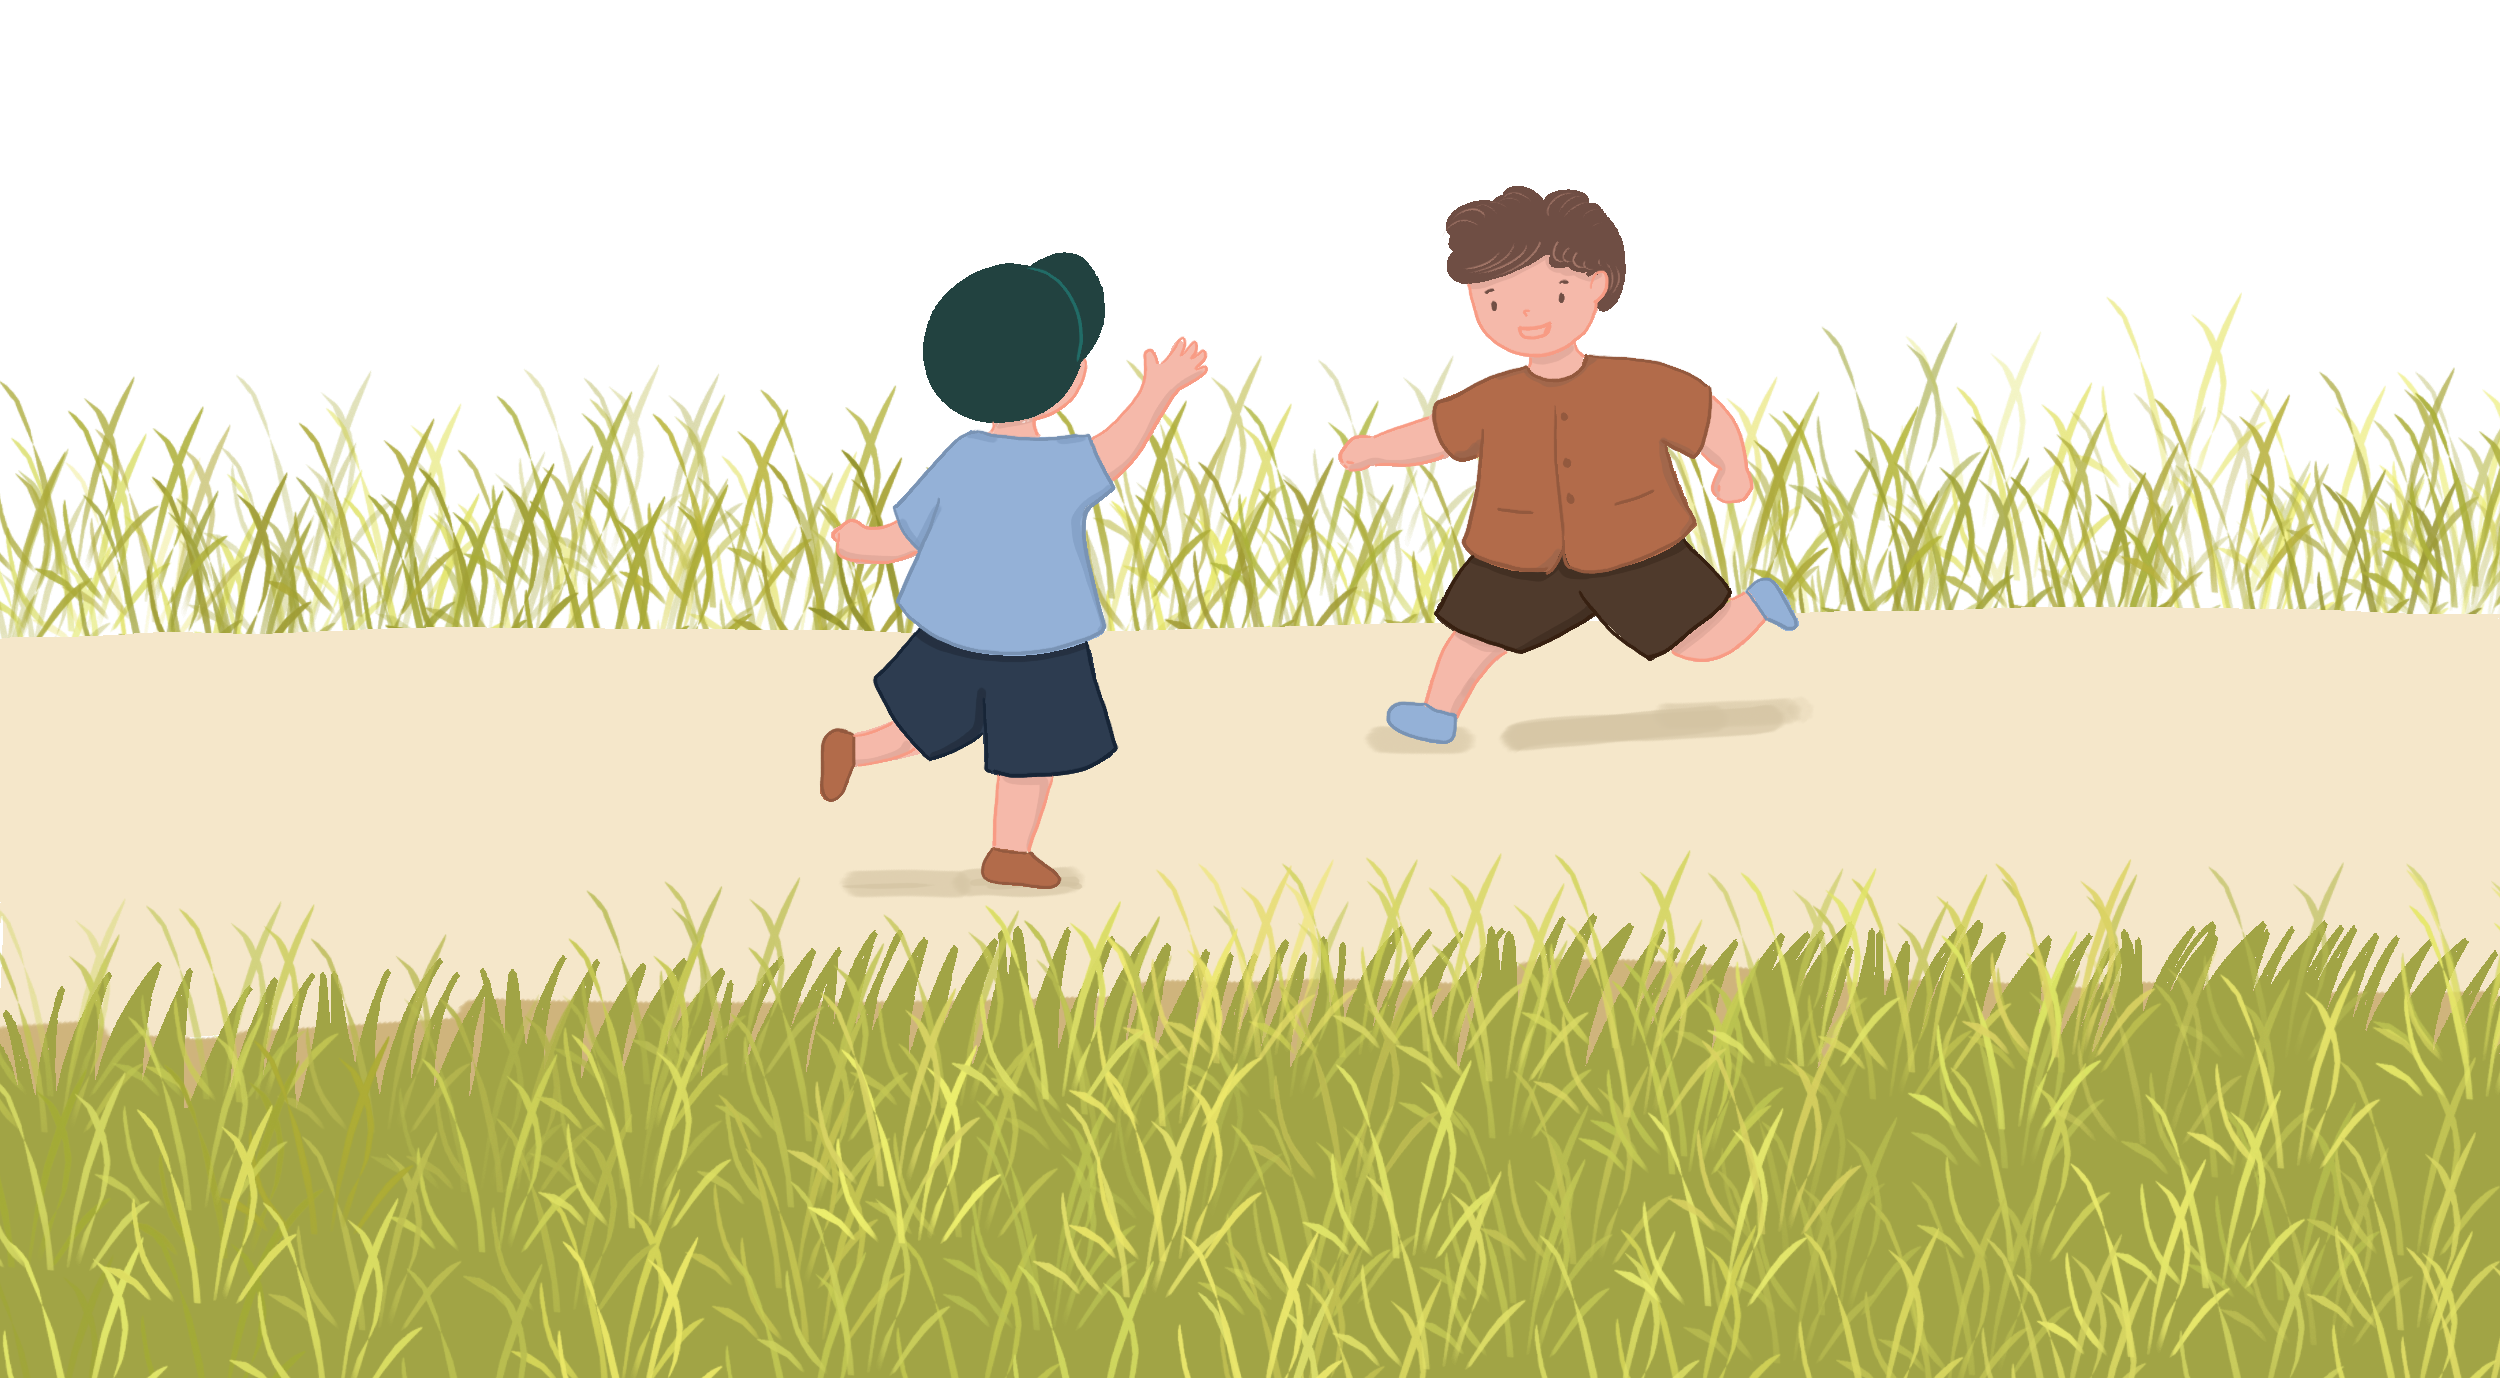
\includegraphics[width=1\linewidth]{Pi3_bai4}
		\vspace*{-15pt}
	\end{figure}
	\textit{Lời giải.} Gọi $a$ (m/phút) là vận tốc của An, còn $b$ (m/phút) là vận tốc của Bình. Giả sử sau khoảng thời gian là $t$ (phút) tính từ lúc khởi hành hai bạn đã gặp nhau. Suy ra
	\begin{align*}
		32a = tb
	\end{align*} 
	và
	\begin{align*}
		18b = ta. 
	\end{align*}
	Nhân hai vế các đẳng thức này với nhau và rút gọn cho $ab$ ta có
	\begin{align*}
		t^2=574.
	\end{align*}
	Từ đó suy ra $t=24$.
	Vậy các bạn đã gặp gỡ nhau sau $12$ phút tính từ lúc khởi hành.
	\vskip 0.1cm
	Cách khác:  Kí hiệu $C$ là điểm hai bạn gặp nhau, do quãng đường tỷ lệ thuận với thời gian đi của mỗi bạn nên tỷ số quãng đường $AC$ và $CB$ là
	$t:18$ đồng thời cũng là $32:t$.
	\begin{figure}[H]
		\vspace*{-5pt}
		\centering
		\captionsetup{labelformat= empty, justification=centering}
		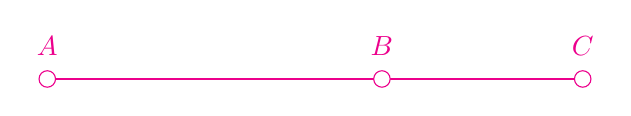
\begin{tikzpicture}[toancuabi,scale=0.85]
			\draw (0,0) -- (8,0);
			\draw (0,0.2) node [above] {$A$};
			\draw (5,0.2) node [above] {$B$};
			\draw (8,0.2) node [above] {$C$};
			\draw [fill=white] (0,0) circle (3.5pt);
			\draw [fill=white] (5,0) circle (3.5pt);
			\draw [fill=white] (8,0) circle (3.5pt);
		\end{tikzpicture}
		\vspace*{-10pt}
	\end{figure}
	Suy ra $t=24$.
	Vậy các bạn đã gặp gỡ nhau sau $12$ phút tính từ lúc khởi hành.
	\vskip 0.1cm
	$\pmb{5.}$ Trong một cuộc thi thể thao do nhà vua Pháp tổ chức, $3$ chàng ngự lâm pháo thủ là Athos, Porthos và Aramis cùng D'Artagnan chia nhau bốn vị trí đầu tiên: $1$, $2$, $3$, $4$ (ứng với giải thưởng: nhất, nhì, ba, bốn). Tổng ba số chỉ vị trí mà Athos, Porthos và D'Artagnan giữ là bằng $6$. Tổng hai số chỉ vị trí mà Porthos và Aramis giữ cũng bằng $6$. Hỏi mỗi chàng ngự lâm đã chiếm các giải nào, biết Porthos chiếm được giải cao hơn Arthos?
	\begin{figure}[H]
		\centering
		\vspace*{-5pt}
		\captionsetup{labelformat= empty, justification=centering}
		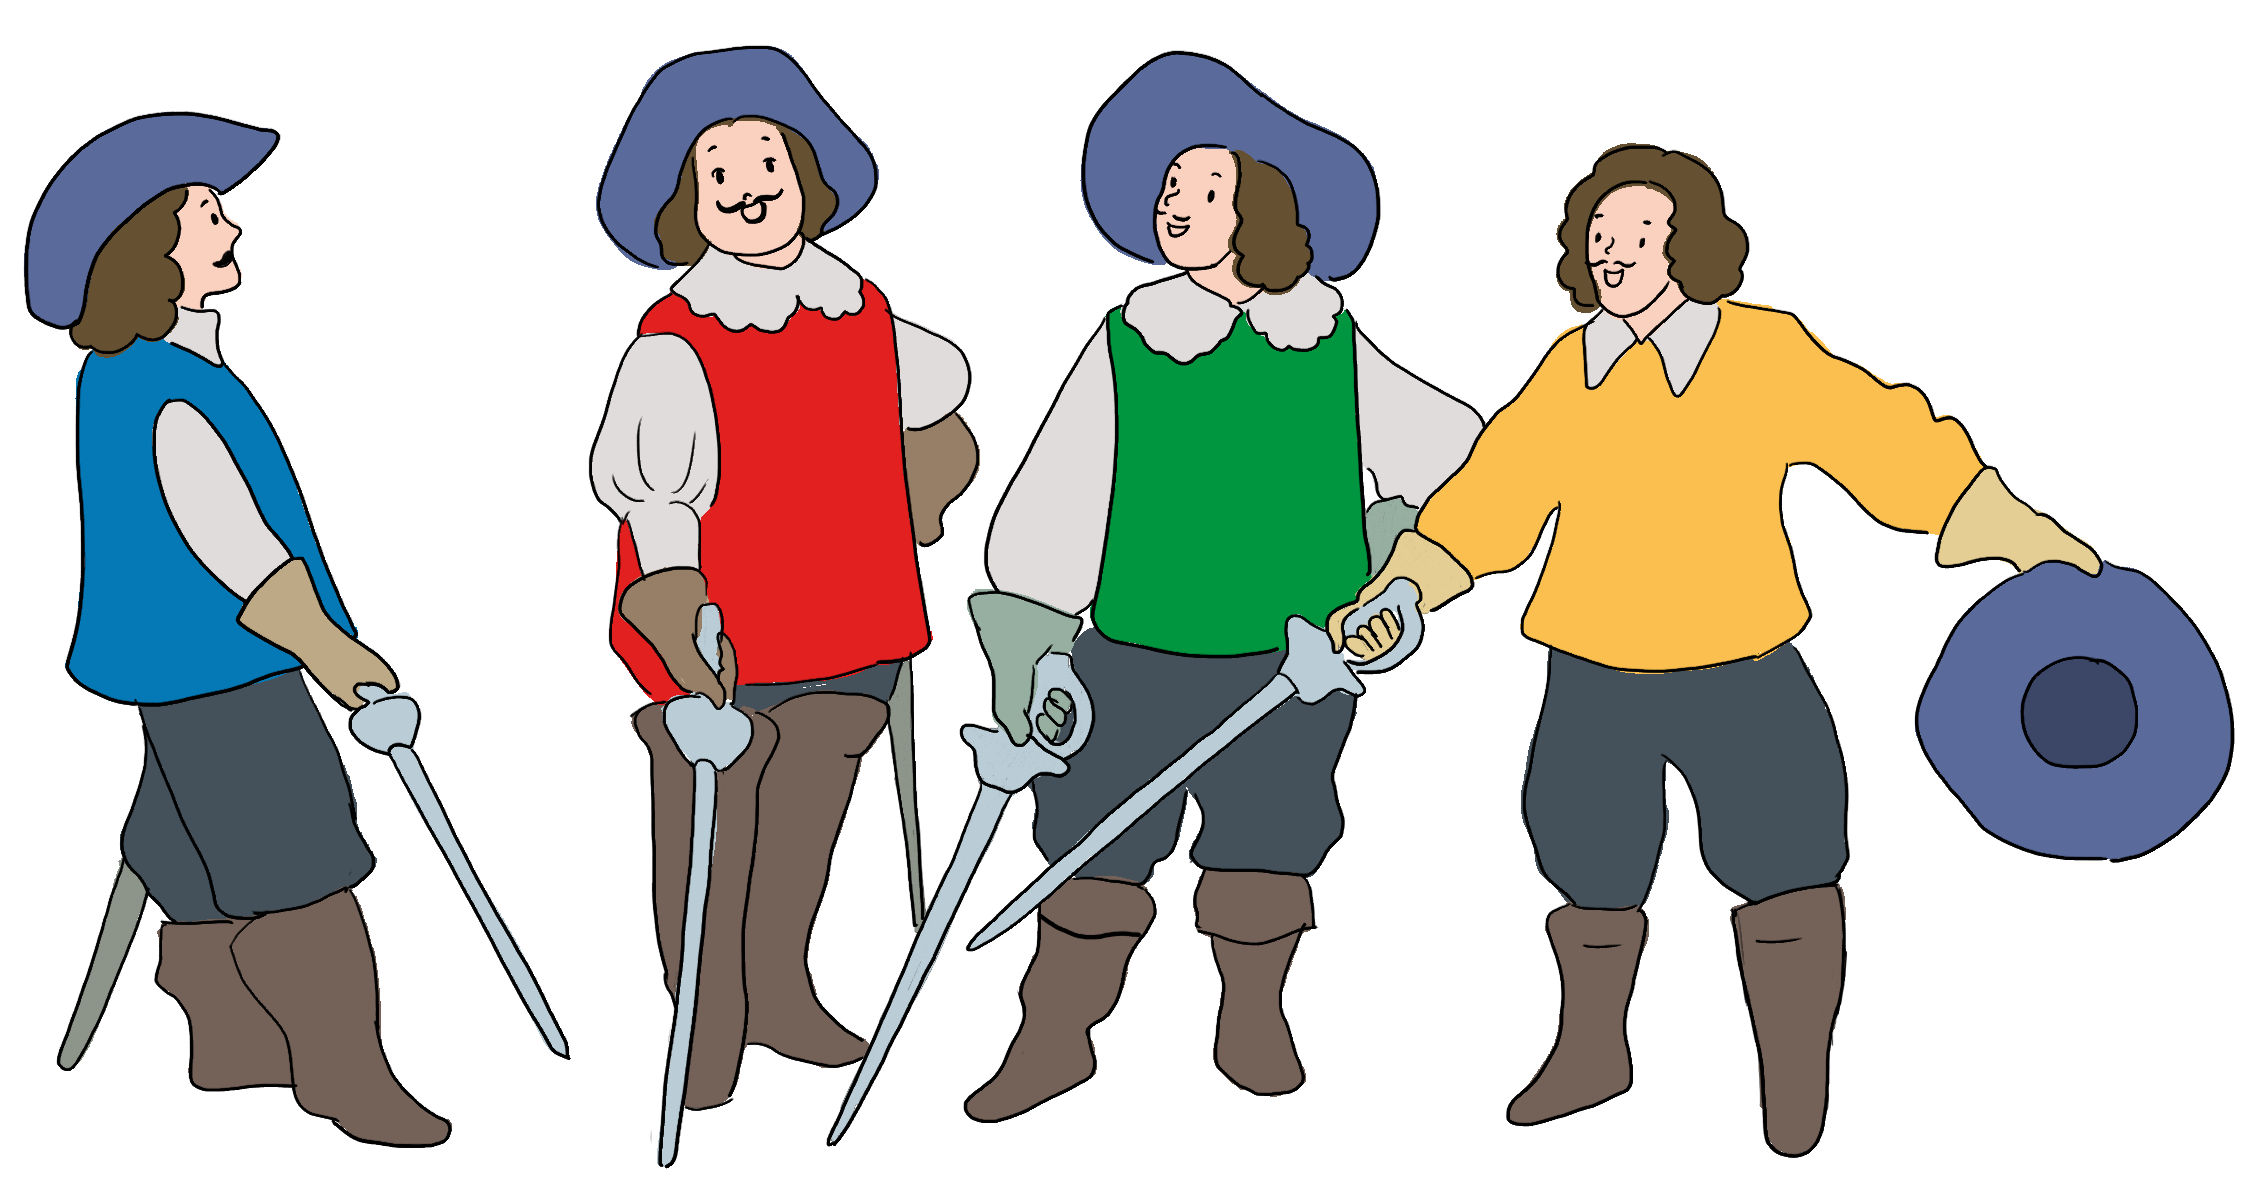
\includegraphics[width=1\linewidth]{Pi3_bai5}
		\vspace*{-15pt}
	\end{figure}
	\textit{Lời giải.} 	Tổng số vị trí của $4$ chàng ngự lâm là 
	\begin{align*}
		1+2+3+4 =10.
	\end{align*} 
	Từ điều kiện đầu tiên suy ra Aramis giữ vị trí thứ 
	\begin{align*}
		10-6 = 4.
	\end{align*}
	Từ điều kiện thứ hai suy ra Porthos giữ vị trí số $2$. Từ điều kiện cuối cùng suy ra Arthos giữ vị thứ thứ $3$, còn D'Artagnan giữ vị trí số~$1$.
	\vskip 0.1cm
	$\pmb{6.}$ Tại một khách sạn nọ, nhân viên trực quản lý điều hành phải làm việc từ $8$h sáng tới $8$h tối (phương án $A$), hoặc từ $8$h tối tới $8$h sáng (phương án $B$), hoặc làm trọn cả ngày $24$h bắt đầu từ $8$h (sáng hoặc tối) (phương án $C$). Nếu làm theo phương án $A$, nhân viên trực quản lý sẽ được nghỉ không ít hơn $1$ ngày ($24$h). Nếu làm theo phương án $B$, nhân viên trực quản lý sẽ được nghỉ không ít hơn $1$ ngày rưỡi ($36$h). Còn nếu làm theo phương án $C$, nhân viên trực quản lý sẽ được nghỉ không ít hơn hai ngày rưỡi ($60$h).
	\vskip 0.1cm
	Hỏi khách sạn phải cần có ít nhất bao nhiêu nhân viên trực quản lý để đảm bảo lịch làm việc, nghỉ ngơi ở trên được tuân thủ?
	\vskip 0.1cm
	\textit{Lời giải.} Rõ ràng thấy rằng khách sạn có thể chỉ cần $4$ nhân viên quản lý để điều hành theo sơ đồ làm việc ``một ngày làm, $3$ ngày nghỉ" theo phương án C--C--C--C.
	\vskip 0.1cm
	Ta sẽ chỉ ra rằng không thể bố trí với số nhân viên ít hơn $4$ người. Thật vậy, nếu có ai đó phải làm cả ngày ($24$h) thì trong thời gian anh ta nghỉ, vì không ai làm việc được quá $1$ ngày liền ($24$h), nên suốt thời gian nghỉ của anh ta là $2{.}5$ ngày, phải có ít nhất $3$ người khác thay phiên nhau làm việc.
	\vskip 0.1cm
	Nếu không có ai làm quá nửa ngày, thì do phải có ai đó làm việc vào ca đêm, nên khi anh ta nghỉ (ít nhất là $1{.}5$ ngày) phải có thêm ít nhất $3$ nhân viên quản lý khác phải làm thay thế.
	\vskip 0.1cm
	Vậy khách sạn cần có ít nhất $4$ nhân viên quản lý trực.
\end{multicols}
%\newpage
%\begingroup
%\thispagestyle{toancuabinone}
%\blfootnote{$^1$\color{toancuabi}Ottawa, Canada.}
%\AddToShipoutPicture*{\put(60,733){
\includegraphics[width=17.2cm]{../mathc.pdf}}}
%%\AddToShipoutPicture*{\put(-2,733){
\includegraphics[width=17.2cm]{../mathl.pdf}}} 
%\AddToShipoutPicture*{\put(66,645){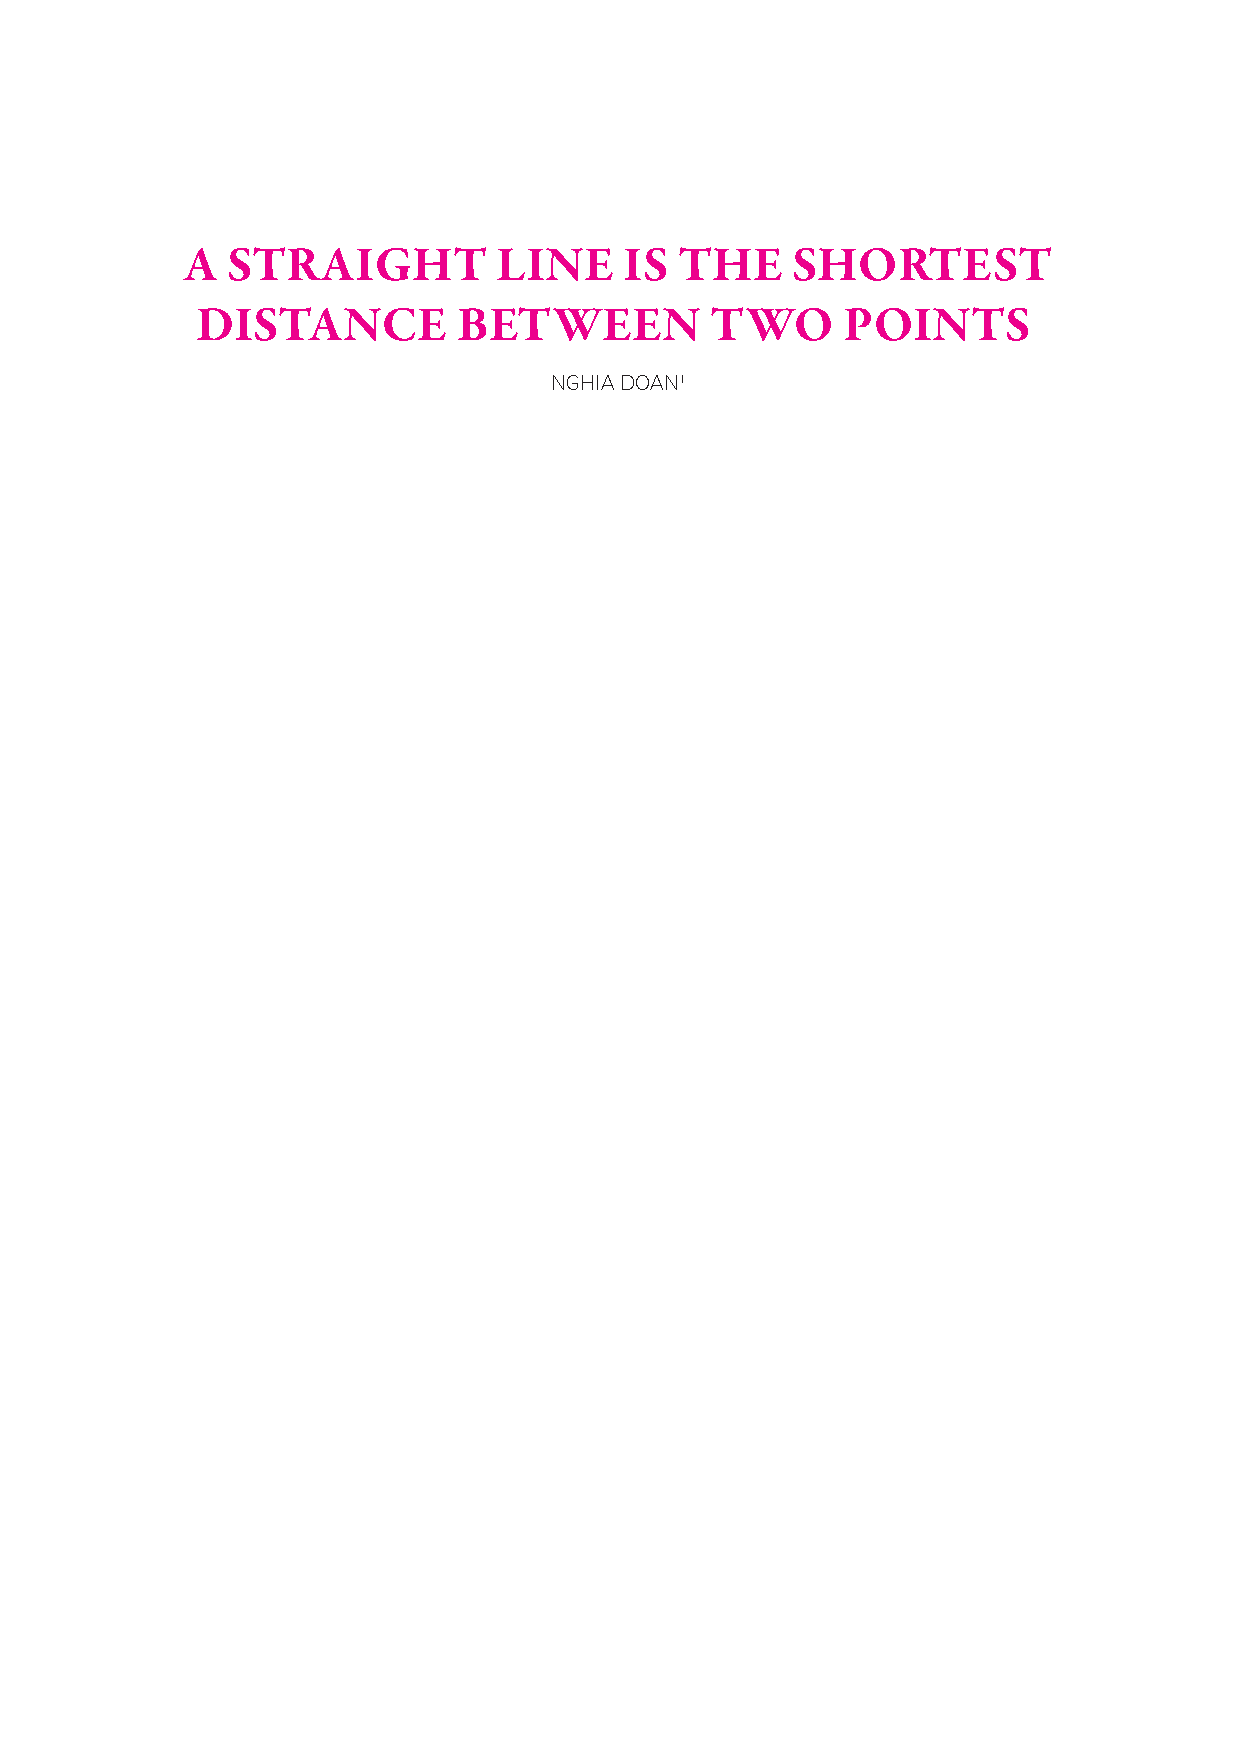
\includegraphics[scale=1]{../tieude5.pdf}}} 
%\centering
%\endgroup
%\graphicspath{{../toancuabi/pic/}}
%\vspace*{60pt}
%
%\begin{multicols}{2}
%	In this article, we explore some basic properties of broken lines.
%	\vskip 0.2cm
%	{\color{toancuabi}\textbf{Fact} (Triangle Inequality)\textbf{.}}
%	For any three points $A,B,C$, 
%	\begin{align*}
%		AB + BC \ge AC,
%	\end{align*}
%	The equality holds if and only if $A, B,$ and $C$ are collinear.
%	\vskip 0.1cm
%	{\color{toancuabi}\textbf{Fact} (Broken Line Inequality)\textbf{.}}
%	For any points $A_1,A_2,\ldots,A_n$, $A_1A_2 + A_2A_3 + \ldots + A_{n-1} A_{n} \ge A_1 A_n.$
%	The equality holds if and only if $A_1,A_2,\ldots,A_{n-1},$ and $A_n$ are collinear.
%	\vskip 0.2cm
%	\PIbox{ {\color{toancuabi}\textbf{Lemma} (Heron's Problem)\textbf{.}}
%		Two points $A$ and $B$ lie on one side of a straight line $l$.
%		$C$ is a point on on $l$.
%		The sum $CA+CB$ is minimal if and only if $C = BC' \cap \ell$, where $B'$ is the reflection of $B$ over $l$.}
%	\vskip 0.2cm
%	\begin{figure}[H]
%		\vspace*{-5pt}
%		\centering
%		\captionsetup{labelformat= empty, justification=centering}
%		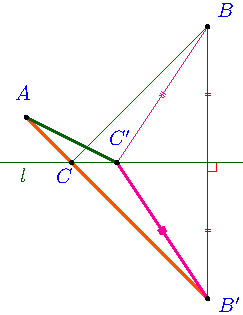
\includegraphics[width= 0.85\linewidth]{heron-problem-1.pdf}
%		\vspace*{-5pt}
%	\end{figure}
%	\vskip 0.1cm
%	\PIbox{ {\color{toancuabi}\textbf{Example} (Cross--section of a cube)\textbf{.}}
%		Lilian cuts a cube with side length $1.$ She got a with a  hexagon cross--section as shown below.
%		What is the minimal value of the hexagon perimeter $AB+BC+CD+DE+EF+FA$?}
%	\begin{figure}[H]
%		\vspace*{-5pt}
%		\centering
%		\captionsetup{labelformat= empty, justification=centering}
%		\includegraphics[width= 1\linewidth]{pi-2023-02-01.pdf}
%		\vspace*{-20pt}
%	\end{figure}
%	\textit{Solution.}
%	The diagram below is obtained by unfolding the cube into a net. The hexagon perimeter forms a broken line $ABCDEFA'.$
%	\begin{figure}[H]
%		\vspace*{-5pt}
%		\centering
%		\captionsetup{labelformat= empty, justification=centering}
%		\includegraphics[width= 0.9\linewidth]{pi-2023-02-02.pdf}
%		\vspace*{-5pt}
%	\end{figure}
%	This is always larger or equal the distance $AA',$ which is same as three times the diagonal of the unit square.
%	Hence the perimeter is always at least ${3\sqrt{2}}.$
%	\vskip 0.2cm
%	\PIbox{{\color{toancuabi}\textbf{Example} (Diagonal of a hexagon)\textbf{.}}		
%		$ABCDEF$ is a convex hexagon, where $\angle A \ge 90\dg$ and $\angle D \ge 90\dg.$
%		Prove that $BC+CE+EF+FB\ge 2AD.$}
%	\vskip 0.2cm
%	\begin{figure}[H]
%		\vspace*{-5pt}
%		\centering
%		\captionsetup{labelformat= empty, justification=centering}
%		\includegraphics[width= 1\linewidth]{pi-2023-02-03.pdf}
%		\vspace*{-10pt}
%	\end{figure}
%	\textit{Proof}.
%	Let $M, N,$ and $P$ be the midpoints of $BF, BE,$ and $CE,$ respectively.
%	Since any broken line is longer or equal the distance between two endpoints, so $AD\le AM+MN+NP+PD.$
%	$MN$ is the median segment in $\triangle BEF,$ thus $FE = 2MN.$ Similarly $BC=2NP.$
%	In $\triangle ABF,$ $\angle A \ge 90\dg,$ thus $BF \ge 2AM.$ Similarly $CE \ge 2DP.$
%	Therefore $BC+CE+EF+FB \ge 2(AM+MN+NP+PD) = 2AD.$
%	\vskip 0.2cm
%	\PIbox{{\color{toancuabi}\textbf{Example} (Romanian Math Olympiad)\textbf{.}}
%		Let $ABCD$ be a convex quadrilateral. It is known that the circles with diameter $AB$ and $CD$ are externally tangent,
%		and so are the circles with diameters $AD$ and $BC.$
%		Prove that $ABCD$ is a rhombus.}
%	\begin{figure}[H]
%		\vspace*{-5pt}
%		\centering
%		\captionsetup{labelformat= empty, justification=centering}
%		\includegraphics[width= 0.8\linewidth]{romanian-pb-gt-40.pdf}
%		\vspace*{-10pt}
%	\end{figure}
%	\textit{Proof}.
%	We first prove a claim.
%	\vskip 0.1cm
%	\textbf{\color{toancuabi}Claim.} Let $M$ and $N$ be the midpoint of $AB$ and $CD$, respectively, then $AD+ BC \ge 2MN.$
%	\vskip 0.1cm
%	\textit{Proof.}
%	Let $E$ be the midpoint of $AC.$ It is easy to see that 
%	\begin{align*}
%		MN \le ME+EN = \frac{BC}{2} + \frac{AD}{2} = \frac{AD+BC}{2}
%	\end{align*}
%	The equality can happen if and only if $MN$ intersect $AC$ at the midpoint of $AC$, so $MN \parallel AD \parallel BC.$
%	\vskip 0.1cm
%	By the claim $AD+BC \ge 2MN, \text{\ similarly\ } AB+CD \ge 2PQ,$ thus 
%	\begin{align*}
%		AB\!+\!BC\!+\!CD\!+\!DA \!\ge\! 2(MN+PQ). \tag{$*$}
%	\end{align*}
%	Now, let $P$ and $Q$ be the midpoints of $BC$ and $AD$, respectively.
%	Since the circles of diameters $AB$ and $CD$ are externally tangent so $AB+CD = 2MN,$ similarly $AD+BC = 2.$
%	Thus 
%	\begin{align*}
%		AB\!+\!BC\!+\!CD\!+\!DA \!=\! 2(MN+PQ). \tag{$**$} 
%	\end{align*}	
%	($**$) implies the existence of equality in ($*$), so $MN \parallel AD \parallel BC$ and $PQ \parallel AB \parallel CD$.
%	Thus $ABCD$ is a parallelogram, and $MN = AD = BC.$ Similarly $AB=CD.$ Since $AB +CD = 2MN$ (see above), therefore
%	\begin{align*}
%		AD = BC = MN = AB = CD.
%	\end{align*}
%	Hence, $ABCD$ is a rhombus.
%\end{multicols}
\newpage
\begingroup
\thispagestyle{toancuabinone}
\blfootnote{$^1$\color{toancuabi}Ottawa, Canada.}
\AddToShipoutPicture*{\put(60,733){\includegraphics[width=17.2cm]{../mathc.pdf}}}
%\AddToShipoutPicture*{\put(-2,733){\includegraphics[width=17.2cm]{../mathl.pdf}}} 
\AddToShipoutPicture*{\put(170,675){\includegraphics[scale=1]{../tieude4.pdf}}} 
\centering
\endgroup
\graphicspath{{../toancuabi/pic/}}
\vspace*{33pt}

\begin{multicols}{2}
	In this article, we explore the use of Venn diagrams through a few examples.
	\vskip 0.2cm
	\PIbox{{\color{toancuabi}\textbf{Example} (Overlapping rugs)\textbf{.}}
		Three rugs have a combined area of $200$ $m^2.$ The rugs are overlapped as shown in the diagram below.
		The overlapped rugs together cover a floor area of $140$ $m^2.$ Furthermore, the area covered by exactly any two rugs is $24$ $m^2$. 
		What is the total area covered by all the rugs?}
	\begin{figure}[H]
		\vspace*{-5pt}
		\centering
		\captionsetup{labelformat= empty, justification=centering}
		\includegraphics[width= 1\linewidth]{pi-2023-01-01.pdf}
		\vspace*{-15pt}
	\end{figure}
	\textit{Solution.}
	The total area of the three rugs, when not overlapping, is the sum of the areas of the three rectangles, which is $200$ $m^2.$
	The region shown in the above diagram is formed by the overlapping rugs and has a total area of $140$ $m^2.$
	This means that $200-140=60$ $m^2$ is the total area of the three \textcolor{red}{red dotted parts}
	(because they are where the rugs overlapped once) plus twice \textcolor{blue}{the blue hatch part}
	(because it is where the rugs overlapped twice).
	\vskip 0.1cm
	In other words, if $r$ and $b$ are the areas of a red dotted and the blue hatch, respectively, then $3r + 2b = 60.$
	Furthermore, since the area of a red dotted part plus the blue hatch part is $24$ $m^2,$ we have $r + b = 24.$
	Therefore $b = 3(r + b)- (3r+2b) = 3 \cdot 24 - 60 = 12.$
	\vskip 0.2cm
	\PIbox{
		{\color{toancuabi}\textbf{Exercise} (Overlapping circles)\textbf{.}}
		Three circles with radii $2$, $3$ and $4$ are overlapping each other.
		The largest circle is partitioned into the shaded region $A$ and two unshaded regions $B$ and $C$.
		If the total area of the shaded regions is $17 \pi$, what is the area of the region $A$?}
	\begin{figure}[H]
		\vspace*{-5pt}
		\centering
		\captionsetup{labelformat= empty, justification=centering}
		\includegraphics[width= 1\linewidth]{pi-2023-01-02.pdf}
		\vspace*{-15pt}
	\end{figure}
	\textit{Solution.}
	The total area of the three circles is the area of the shaded regions plus \textit{twice} the area of the unshaded regions:
	\begin{align*}
		&4\pi + 9\pi + 16\pi = 17\pi + 2(B+C) \\
		\Rightarrow \,&B+C = 6\pi \\
		\Rightarrow \,&A = 16\pi - (B+C) = 10\pi
	\end{align*}
	\vskip 0.2cm
	\PIbox{{\color{toancuabi}\textbf{Example} (Alligators are ferocious and creepy crawlers)\textbf{.}}
		If all alligators are ferocious creatures and some creepy crawlers are alligators. It is easy to verify that:
		(i) all alligators are creepy crawlers; (ii) some ferocious creatures are creepy crawlers;
		and (iii) some alligators are not creepy creatures.}
	
	\PIbox{
		Now, which statements below are true, false, or undecidable (you can't say it is true or false)?
		\vskip 0.1cm
		$S1.$ Some of creepy creatures are ferocious.
		\vskip 0.1cm
		$S2.$ Some ferocious creatures are creepy crawlers.
		\vskip 0.1cm
		$S3.$ Some alligators are not creepy creatures.
		\vskip 0.1cm
		$S4.$ Some ferocious crawlers are not alligators.
		\vskip 0.1cm
		$S5.$ Alligators are ferocious and creepy crawlers.}
	\vskip 0.2cm
	\textit{Solution.}
	To help the reasoning with visual cues, you can use Venn diagrams.
	\vskip 0.1cm
	First, we draw a \textcolor{red}{red circle} depicting the set of alligators. In other words all alligators are in this circle.
	Since all alligators are ferocious creatures, thus the \textcolor{blue}{blue circle} containing all ferocious creatures must cover the circle of alligators .
	Now, some creepy crawlers are alligators, thus the \textcolor{green}{green circle} containing all creepy crawlers must intersect and not contain the circle of alligators.
	Logically the circle of creepy crawlers then should intersect the circle of ferocious creatures and should not cover it.
	We get the diagram shown below.
	\begin{figure}[H]
		\vspace*{-5pt}
		\centering
		\captionsetup{labelformat= empty, justification=centering}
		\includegraphics[width= 1\linewidth]{pi-2023-01-03.pdf}
		\vspace*{-10pt}
	\end{figure}
	For $S1,$ those creepy crawlers are alligators, they must be in the intersection of the \textcolor{red}{red circle} and \textcolor{green}{green circle}.
	Since the \textcolor{red}{red circle} resides within of the \textcolor{blue}{blue circle} the intersection must be part of the \textcolor{blue}{blue circle}.
	In other words, those creepy crawlers are ferocious creatures. Thus the statement $S1$ is true.
	\vskip 0.1cm
	It is also easy to verify that $S2$ is true.
	\vskip 0.1cm
	Since we know that \textit{some creepy crawlers are alligators}, thus the \textcolor{green}{green circle} intersect
	and may not contain the whole the \textcolor{red}{red circle}, thus $S2$ is \textit{undecidable.}
	We don't know if some alligators are not creepy.
	\vskip 0.1cm
	The remaining two statements $S4$ and $S5$ are both \textit{undecidable}. Try to prove it yourself.
	\vskip 0.1cm
	\PIbox{{\color{toancuabi}\textbf{Exercise} (Are boys good at math)\textbf{.}}
		Let us assume that \textit{all boys in the math club are good at math.} 
		Which of the following statements must be true?
		\vskip 0.1cm
		$S1.$ No boy whose math is not good is a member of the math club.
		\vskip 0.1cm
		$S2.$ All boys whose math is good are members of the math club.
		\vskip 0.1cm
		$S3.$ All boys who are not members of the math club are not good at math.
		\vskip 0.1cm
		$S4.$ Every member of the math club whose math is good is a boy.
		\vskip 0.1cm
		$S5.$ There is one boy in the math club whose math is not good.
		\vskip 0.1cm
		Now decide whether the following is true or false.
		\textit{A girl is good at math as a boy who is not member of the math club is not good as math as a boy who is member of the math club.}}
	\vskip 0.1cm
	\textit{Solution.}
	Draw three circles that are pairwise intersecting. One circle is labeled \textit{boys}; the girls are outside of this circle. One circle is labeled \textit{math} meaning whoever in this circle is good at math; the students outside of this circle are not good at math. One circle is labeled \textit{club} meaning whoever in this circle is a member of the math club; the students outside of this circle are not members of the math club.
	None of the circles can contain another one. The \textit{club} circle must contain the inversection of the \textit{boys} circle and the \textit{math} circle.
	A diagram is shown below.
	\begin{figure}[H]
		%			\vspace*{-5pt}
		\centering
		\captionsetup{labelformat= empty, justification=centering}
		\includegraphics[width= 1\linewidth]{pi-2023-01-04.pdf}
		\vspace*{-10pt}
	\end{figure}
	For $S2,$ $S3,$ $S4,$ and $S5,$ it is easy to find a counterexample, thus none of them is true.
	The statement $S1$ means that if a boy is not good at math, then he is not a member of the math club. This is obviously true. We conclude that $S1$ is true.
	\vskip 0.1cm
	\columnbreak
	\PIbox{
	\centerline{\textbf{\color{toancuabi}Vocabulary}}
	\vskip 0.1cm
	{\color{toancuabi}Venn diagram (n):} sơ đồ Venn, biểu đồ Venn
	\vskip 0.1cm
	{\color{toancuabi}intersection (n):} phần giao nhau
	\vskip 0.1cm
	{\color{toancuabi}overlapping (adj):} chồng lên nhau
	\vskip 0.1cm
	{\color{toancuabi}furthermore (adv):} hơn nữa
	\vskip 0.1cm
	{\color{toancuabi}undecidable (adj):} không xác định được tính đúng/sai
	\vskip 0.1cm
	{\color{toancuabi}suppose (v):} giả sử 
	\vskip 0.1cm
	{\color{toancuabi}suppose by contradiction (v):} giả sử bằng phản chứng 
	\vskip 0.1cm
	{\color{toancuabi}rug (n):} tấm thảm
	\vskip 0.1cm
	{\color{toancuabi}alligator (n):} cá sấu
	\vskip 0.1cm
	{\color{toancuabi}ferocious (adj):} hung dữ
	\vskip 0.1cm
	{\color{toancuabi}creepy (adj):} rùng rợn
	\vskip 0.1cm
	{\color{toancuabi}crawler (n):} loài bò sát
	\vskip 0.1cm
	{\color{toancuabi}creature (n):} sinh vật}
\end{multicols}
\newpage
\begingroup
\blfootnote{$^1$\color{toancuabi}Trường Liên cấp Hội nhập Quốc tế iSchool Quảng Trị.}
\AddToShipoutPicture*{\put(48,680){\includegraphics[scale=1]{../tieude10.pdf}}}   
\centering
\endgroup
\vspace*{30pt} 

\begin{multicols}{2}
	\textbf{\color{toancuabi}Ayatori} (hay trò chơi dây) là một trò chơi mà khi nhắc đến chắc chắn những người hâm mộ bộ truyện tranh Doraemon đều biết đến và nhớ ngay tới nhân vật Nobita. Trò chơi Ayatori là một trò chơi rất thú vị, người chơi sẽ sử dụng một sợi dây được buộc thành hình tròn, sau đó dùng những ngón tay của mình đan xen các sợi dây để tạo ra nhiều hình dạng khác nhau từ đơn giản đến phức tạp. Hôm nay, em hãy thử xếp hình ngôi sao thông qua trò chơi Ayatori nhé!
	\vskip 0.1cm
	\textit{Bước} $1$: Cách cầm dây khi mới bắt đầu chơi trò chơi Ayatori là giữ sợi dây trong ngón cái và ngón út bằng hai tay, rồi kéo ngang để chuẩn bị chơi.
	\begin{figure}[H]
		\vspace*{-10pt}
		\centering
		\captionsetup{labelformat= empty, justification=centering}
		\includegraphics[width=0.81\linewidth]{1a}
		
		\vspace*{1pt}
		\includegraphics[width=0.81\linewidth]{1b}
		
		\vspace*{1pt}
		\hspace*{1pt}\includegraphics[width=0.81\linewidth]{1c}
		\vspace*{-10pt}
	\end{figure}
	\textit{Bước} $2$: Thả dây ở hai ngón tay út. Sau đó dùng hai ngón tay út luồn phía dưới sợi dây ở hai ngón cái để kéo sợi dây ra như hình vẽ.
	\begin{figure}[H]
		\vspace*{-5pt}
		\centering
		\captionsetup{labelformat= empty, justification=centering}
		\includegraphics[width=0.81\linewidth]{2a}
%		\vspace*{-5pt}
	\end{figure}
	\begin{figure}[H]
		\vspace*{5pt}
		\centering
		\captionsetup{labelformat= empty, justification=centering}
		\includegraphics[width=0.81\linewidth]{2b}
		\vspace*{-10pt}
	\end{figure}
	\textit{Bước} $3$: Lấy ngón trỏ tay phải móc vào phần dây giữa ngón cái và ngón út của tay trái. Thực hiện tương tự với ngón trỏ tay trái.
	\begin{figure}[H]
		\vspace*{-5pt}
		\centering
		\captionsetup{labelformat= empty, justification=centering}
		\includegraphics[width=0.81\linewidth]{3a}
		
		\vspace*{1pt}
		\includegraphics[width=0.81\linewidth]{3b}
			
		\vspace*{1pt}
		\includegraphics[width=0.81\linewidth]{3c}
				
		\vspace*{1pt}
		\hspace*{1pt}\includegraphics[width=0.81\linewidth]{3d}
		\vspace*{-10pt}
	\end{figure}
	\textit{Bước} $4$: Thả dây ở hai ngón tay út.
	\begin{figure}[H]
		\vspace*{-5pt}
		\centering
		\captionsetup{labelformat= empty, justification=centering}
		\includegraphics[width= 0.81\linewidth]{4}
		\vspace*{-10pt}
	\end{figure}
	\textit{Bước} $5$: Dùng ngón út để kéo sợi dây ở dưới cùng lên và chúng ta sẽ hoàn hành ngôi sao năm cánh.
	\begin{figure}[H]
		\vspace*{5pt}
		\centering
		\captionsetup{labelformat= empty, justification=centering}
		\includegraphics[width= 0.81\linewidth]{5}
		\vspace*{-5pt}
	\end{figure}
	Hãy thử suy ngẫm xem hình ngôi sao năm cánh em vừa tạo ra có bao nhiêu trục đối xứng?
	\vskip 0.1cm
	\textbf{\color{toancuabi}Làm cây thông Noel}
	\vskip 0.1cm
	\textit{Bước} $1$: Xếp hai tờ giấy màu cứng chồng lên nhau rồi gấp đôi lại cho đều nhau. Sau đó lấy bút vẽ phác họa hình cây thông lên mặt ngoài của tờ giấy rồi dùng kéo cắt theo các đường đã vẽ sẵn. Lúc mở ra, em sẽ có hai cây thông với kích thước giống nhau.
	\begin{figure}[H]
		\vspace*{-5pt}
		\centering
		\captionsetup{labelformat= empty, justification=centering}
		\includegraphics[width= 1\linewidth]{6}
		\vspace*{-15pt}
	\end{figure}
	\textit{Bước} $2$: Gấp đôi cây thông theo chiều ngang, gấp đầu nhọn xuống dưới để xác định tâm của mỗi cây thông. Tiếp đến dùng kéo cắt một đường từ đỉnh cây thông xuống điểm vừa đánh dấu. Cây thông còn lại thì cắt từ đáy lên điểm vừa đánh dấu.
	\begin{figure}[H]
		\vspace*{-5pt}
		\centering
		\captionsetup{labelformat= empty, justification=centering}
		\includegraphics[width= 1\linewidth]{7}
		\vspace*{-15pt}
	\end{figure}
	\textit{Bước} $3$: Sau khi đã hoàn thành việc cắt hai cây thông, em hãy ghép chúng lại với nhau theo các khe đã cắt, chú ý để các góc không bị cong. Nếu sau khi ráp cây thông bị lung lay các em có thể cố định lại bằng keo dán.
	\begin{figure}[H]
		\vspace*{-5pt}
		\centering
		\captionsetup{labelformat= empty, justification=centering}
		\includegraphics[width= 1\linewidth]{8}
		\vspace*{-15pt}
	\end{figure}
	\textit{Bước} $4$: Cuối cùng các em chỉ cần điều chỉnh sao cho cây thông đứng vững, trang trí thêm các dây ruy băng hay rắc kim tuyến,... hoặc vẽ họa tiết lên cây thông Noel để nhìn đẹp hơn.
	\begin{figure}[H]
		\vspace*{-5pt}
		\centering
		\captionsetup{labelformat= empty, justification=centering}
		\includegraphics[height= 0.31\linewidth]{9a}
		\includegraphics[height= 0.31\linewidth]{9b}
		\includegraphics[height= 0.31\linewidth]{9c}
		\caption{\small\textit{\color{toancuabi}Ảnh: Internet.}}
		\vspace*{-10pt}
	\end{figure}
	\textbf{\color{toancuabi}Bài tập}
	\vskip 0.1cm
	Còn gì tuyệt vời hơn khi được thả diều dưới bầu trời xanh và trong làn gió mát của những buổi chiều mùa hè oi ả. Bằng những kiến thức của bài ``Hình có trục đối xứng" và trí tưởng tượng phong phú của mình, em hãy tự làm ra cho mình một con diều đẹp đẽ với màu sắc rực rỡ nhé. Chúc em thành công!
	\begin{figure}[H]
			\vspace*{-5pt}
			\centering
			\captionsetup{labelformat= empty, justification=centering}
			\includegraphics[width= 1\linewidth]{10}
			\caption{\small\textit{\color{toancuabi}Hình ảnh con diều (Ảnh: Internet)}}
			\vspace*{-5pt}
		\end{figure}
\end{multicols}
%	\newpage 

	\setcounter{figure}{0}
	\thispagestyle{thachthuctoanhocnone}
\pagestyle{thachthuctoanhoc}
\everymath{\color{thachthuctoanhoc}}
\graphicspath{{../thachthuctoanhoc/pic/}}
\begingroup
\AddToShipoutPicture*{\put(0,616){\includegraphics[width=19.3cm]{../thachthuctoanhoc/bannerthachthuc}}}
\centering
\vspace*{4cm}
\endgroup
\vspace*{-8pt}
\begin{tBox}
	\begin{itemize}[leftmargin = 13pt, itemsep = 1.0pt] 
		\item Mỗi bài toán đề xuất (kèm theo lời giải) cần được nêu rõ là bài sáng tác hay bài sưu tầm.
		%		\item Mỗi bài toán đề xuất (kèm theo lời giải) cần được nêu rõ là bài sáng tác hay bài sưu tầm (nếu là bài sưu tầm, cần ghi rõ nguồn).
		\item Bài giải cho mỗi bài toán cần được trình bày trong một file riêng hoặc
		một tờ giấy riêng.
		\item  Người đề xuất bài toán hoặc gửi bài giải cho các bài toán trong mục ``Thách thức kỳ này" cần ghi rõ họ, đệm, tên và nơi làm việc/học tập, số điện thoại liên hệ. Nếu là học sinh (hoặc sinh viên) cần ghi rõ là học sinh lớp mấy (hoặc sinh viên năm thứ mấy).
		\item Các bài toán trong mục Thách thức kỳ này hướng tới các độc giả là học sinh phổ thông; được phân chia thành các mức độ $B$, $A$, và được sắp xếp theo độ khó tăng dần, theo đánh giá chủ quan của Ban biên tập. Các bài toán mức độ $B$ không đòi hỏi các kiến thức vượt quá chương trình môn Toán cấp THCS; các bài toán mức độ $A$ không đòi hỏi các kiến thức vượt quá chương trình môn Toán cấp THPT.
		\item Cách thức gửi bài toán đề xuất hoặc lời giải: gửi file thu được bằng cách scan, ảnh chụp (rõ nét) của bản viết tay, hoặc được soạn thảo bằng các phần mềm Latex, Word tới \url{bbt@pi.edu.vn} hoặc gửi qua đường bưu điện tới Tòa soạn (xem địa chỉ tại bìa $2$).
		\item Hạn gửi lời giải cho các bài toán P$711$--P$720$: trước ngày $15/7/2023$.
	\end{itemize}
\end{tBox}
\begin{center}
	\vspace*{-5pt}
	\textbf{\color{thachthuctoanhoc}\color{thachthuctoanhoc}\color{thachthuctoanhoc}THÁCH THỨC KỲ NÀY}
	\vspace*{-5pt}
\end{center}
\begin{multicols}{2}
	\setlength{\abovedisplayskip}{4pt}
	\setlength{\belowdisplayskip}{4pt}
	{\color{thachthuctoanhoc}{\usefont{T5}{qag}{b}{n} P711.}}
	(Mức $B$) Bác An có $6$ tấm thẻ $A,$ $B,$ $C,$ $D,$ $E,$ $F$. Bác ghi các số nguyên dương $1,$ $2,$ $3,$ $4,$ $5,$ $6$ lên mỗi tấm thẻ, sao cho mỗi thẻ được ghi một số và không có hai thẻ nào có số giống nhau. Biết rằng tổng các số ghi ở các tấm thẻ $A,$ $B,$ $C$ bằng $14$ và tổng các số được ghi ở các tấm thẻ $A,$ $D,$ $E$ là $12$. Hỏi bác An có bao nhiêu cách ghi số như vậy?
	\vskip 0.3cm
	\hfill	\textit{Nguyễn Tường Thanh, Hải Dương}
	\vskip 0.3cm
	{\color{thachthuctoanhoc}{\usefont{T5}{qag}{b}{n} P712.}}
	(Mức $B$) Tìm tất cả các số nguyên $a$ sao cho $a^2+a+1$ chỉ có ước nguyên tố không vượt quá $5$. 
	\begin{flushright}
		\textit{Hà Duy Hưng, Hà Nội}
	\end{flushright}
	{\color{thachthuctoanhoc}{\usefont{T5}{qag}{b}{n} P713.}}
	(Mức $B$) Xác định tất cả các cặp số thực $(a;b)$ sao cho $a+b$ là số nguyên và $a^3+b^3=2$. 
	\vskip 0.1cm
	\hfill	\textit{Nguyễn Đức Tấn, Tp. Hồ Chí Minh}
	\vskip 0.1cm
	{\color{thachthuctoanhoc}{\usefont{T5}{qag}{b}{n} P714.}}
	(Mức $B$) Cho $2023$ số nguyên dương $a_1,$ $a_2,$ $\ldots,$ $a_{2023}$ thỏa mãn
	\begin{align*}
		\frac{1}{a_1^2}+\frac{1}{a_2^2}+\cdots+\frac{1}{a_{2023}^2}\ge 33.
	\end{align*}
	Chứng minh rằng, trong $2023$ số đó, luôn tìm được ít nhất $21$ số bằng nhau.  
	\vskip 0.1cm
	\hfill	\textit{Nguyễn Văn Quý, Hà Nội (st)}
	\vskip 0.1cm
	{\color{thachthuctoanhoc}{\usefont{T5}{qag}{b}{n} P715.}}
	(Mức $B$) Cho tam giác không cân $ABC$ nội tiếp đường tròn $(O)$, có $M$ là trung điểm $BC$. Đường tròn ngoại tiếp tam giác $AMO$ cắt đường tròn $(O)$ tại điểm thứ hai $D$. Đường thẳng $AM$ cắt $(O)$  tại điểm thứ hai $E$. Chứng minh rằng $DE\| BC$. 
	\begin{center}
		\definecolor{qqqqff}{rgb}{0,0,1}
		\definecolor{qqqqffa}{rgb}{1,1,1}
		\definecolor{cqcqcq}{rgb}{0.7529411764705882,0.7529411764705882,0.7529411764705882}
		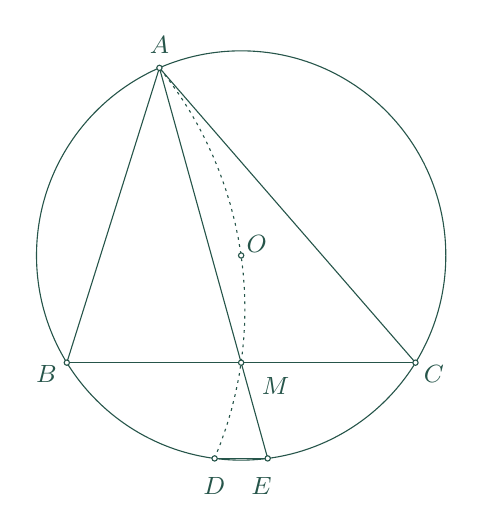
\begin{tikzpicture}[thachthuctoanhoc,scale=0.6, node font=\small]
			\draw  (-3.26,4.44)-- (-5.22,-1.8);
			\draw  (-5.22,-1.8)-- (2.16,-1.8);
			\draw  (2.16,-1.8)-- (-3.26,4.44);
			\draw  (-1.53,0.4687820512820516) circle (4.331682351721972cm);
			\draw  (-2.0917832603951787,-3.826316499922491)-- (-0.9682167396048218,-3.8263164999224912);
			\draw  (-3.26,4.44)-- (-0.9682167396048218,-3.8263164999224912);
			\draw [shift={(-9.556965317919069,-0.665608974358972)},dash pattern=on 1pt off 1.6pt]  plot[domain=-0.40050890991965815:0.6812945286306901,variable=\t]({1*8.106726541220599*cos(\t r)+0*8.106726541220599*sin(\t r)},{0*8.106726541220599*cos(\t r)+1*8.106726541220599*sin(\t r)});
			\draw [fill=white] (-3.26,4.44) circle (1.6pt);
			\draw (-3.26,4.93) node {$A$};
			\draw [fill=white] (-5.22,-1.8) circle (1.6pt);
			\draw (-5.65,-2.05) node {$B$};
			\draw [fill=white] (2.16,-1.8) circle (1.6pt);
			\draw (2.55,-2.05) node {$C$};
			\draw [fill=white] (-1.53,0.4687820512820516) circle (1.6pt);
			\draw (-1.2,0.71) node {$O$};
			\draw [fill=white] (-1.53,-1.8) circle (1.6pt);
			\draw (-0.8,-2.3) node {$M$};
			\draw [fill=white] (-2.0917832603951787,-3.826316499922491) circle (1.6pt);
			\draw (-2.1,-4.4) node {$D$};
			\draw [fill=white] (-0.9682167396048218,-3.8263164999224912) circle (1.6pt);
			\draw (-1.1,-4.4) node {$E$};
		\end{tikzpicture}
	\end{center}
	\begin{flushright}
		\textit{Bằng Linh, Phú Thọ (st)}
	\end{flushright}
	{\color{thachthuctoanhoc}{\usefont{T5}{qag}{b}{n} P716.}}
	(Mức $B$) Trong một lớp học có $33$ học sinh. Mỗi bạn viết lên bảng số người trong lớp có cùng tên với mình và viết lên bảng số người có cùng họ với mình (không tính bản thân người đó). Sau khi tất cả học sinh hoàn thành việc viết số, thì trên bảng mỗi số $0,1,2,\ldots,10$ đều xuất hiện ít nhất một lần. Hỏi số $6$ xuất hiện bao nhiêu lần?
	\begin{flushright}
		\textit{Tô Trung Hiếu, Nghệ An (st)}
	\end{flushright}
	{\color{thachthuctoanhoc}{\usefont{T5}{qag}{b}{n} P717.}}
	(Mức $A$) Chứng minh rằng, với mọi bộ ba số thực $(a;b;c)$ thoả mãn  $ac\ne0$ và $b^2\ge4ac$, ta có
	\begin{align*}
		(a-b)^4+(b-c)^4+(c-a)^4 \ge \dfrac{81}{128}c^4.
	\end{align*}
	\begin{flushright}
		\textit{Nguyễn Văn Long, Vĩnh Phúc}
	\end{flushright}
	{\color{thachthuctoanhoc}{\usefont{T5}{qag}{b}{n} P718.}}
	(Mức $A$) Cho tam giác $ABC$ và $P$ là một điểm cố định nằm trong tam giác đó. Một đường thẳng $d$ quay quanh điểm $P$, cắt các đường thẳng $BC,CA,AB$ tương ứng tại các điểm $D,E,F$. Gọi $Q$ là giao điểm thứ hai của hai đường tròn $(ADE)$ và $(APF)$. Chứng minh rằng, $Q$ luôn thuộc một đường tròn cố định.  
	\begin{center}
		\definecolor{ffqqqq}{rgb}{1,0,0}
		\definecolor{qqqqff}{rgb}{0,0,1}
		\definecolor{qqqqffa}{rgb}{1,1,1}
		\begin{tikzpicture}[thachthuctoanhoc, scale=0.65, node font= \small]
			\draw  (-4.76,5.36)-- (-6.22,-0.5);
			\draw  (-6.22,-0.5)-- (0.2,-0.5);
			\draw  (0.2,-0.5)-- (-4.76,5.36);
			\draw [color=ffqqqq] (-5.222691037714135,1.894862071043978) circle (3.4958924272738447cm);
			\draw  (-5.750222132850728,2.8374132314498297) circle (2.709978575054024cm);
			\draw  (-7.76943396226415,-0.5)-- (-1.7287290671233002,1.7787000672061575);
			\draw  (-7.76943396226415,-0.5)-- (-6.22,-0.5);
			\draw [fill=white] (-4.76,5.36) circle (1.6pt);
			\draw (-4.76,5.73) node {$A$};
			\draw [fill=white] (-6.22,-0.5) circle (1.6pt);
			\draw (-6.36,-0.87) node {$B$};
			\draw [fill=white] (0.2,-0.5) circle (1.6pt);
			\draw (0.26,-0.81) node {$C$};
			\draw [fill=white] (-3.74,1.02) circle (1.6pt);
			\draw (-3.5,0.65) node {$P$};
			\draw [fill=white] (-7.76943396226415,-0.5) circle (1.6pt);
			\draw (-8.1,-0.73) node {$D$};
			\draw [fill=white] (-1.7287290671233002,1.7787000672061575) circle (1.6pt);
			\draw (-1.34,1.95) node {$E$};
			\draw [fill=white] (-6.059271801059053,0.14511455191366746) circle (1.6pt);
			\draw (-6.3,0.5) node {$F$};
			\draw [fill=white] (-8.418223065252786,3.3125499506724045) circle (1.6pt);
			\draw (-8.82,3.53) node {$Q$};
		\end{tikzpicture}
	\end{center}
	\begin{flushright}
		\textit{Phạm Vĩnh Minh, Đồng Tháp}
	\end{flushright}
	{\color{thachthuctoanhoc}{\usefont{T5}{qag}{b}{n} P719.}}
	(Mức $A$) Cho $S$ là một tập hữu hạn các số nguyên lớn hơn $1$ thoả mãn: với mỗi số nguyên dương $n$, tồn tại $x\in S$ sao cho  hoặc $x,n$ nguyên tố cùng nhau, hoặc $n$ chia hết cho $x$.  Chứng minh rằng, tồn tại $x,y\in S$ (có thể $x=y$) sao cho ước chung lớn nhất của $x,y$ là một số nguyên tố. 
	\begin{flushright}
		\textit{Bằng Linh, Phú Thọ (st)}
	\end{flushright}
	{\color{thachthuctoanhoc}{\usefont{T5}{qag}{b}{n} P720.}}
	(Mức $A$) Một thành phố có $1332$ căn nhà. Mỗi dịp Noel, ông già Noel sẽ đến thăm các căn nhà đó theo thứ tự tùy ý. Chứng minh rằng, có thể tìm được $12$ căn nhà trong thành phố đó sao cho trong $3$ năm liên tiếp, có ít nhất $2$ năm mà ông già Noel đến thăm $12$ căn nhà đó theo cùng một thứ tự.
	\begin{flushright}
		\textit{Trương Bảo Nam, Hà Nội}
	\end{flushright}
	\textbf{\color{thachthuctoanhoc}ĐÍNH CHÍNH}
	\vskip 0.05cm
	$\bullet$ Trong phát biểu của bài toán {\color{thachthuctoanhoc}{\usefont{T5}{qag}{b}{n} P685}} tập $7$ số $3$, câu ``Cho $2023$ hình có tổng diện tích lớn hơn $2023$" đổi thành ``Cho $2023$ hình có tổng diện tích lớn hơn $2022$".
	\vskip 0.05cm
	$\bullet$ Trong phát biểu của bài toán {\color{thachthuctoanhoc}{\usefont{T5}{qag}{b}{n} P707}} tập $7$ số $5$, công thức của $a$ bị thiếu số $x$, công thức đúng là:
	\begin{align*}
		a=\left\lfloor x+\dfrac12\right\rfloor+\left\lfloor\sqrt{2}x\right\rfloor.
	\end{align*} 
	Thành thật cáo lỗi cùng bạn đọc.
\end{multicols}
\newpage
\centerline{{\large{\textbf{\color{thachthuctoanhoc}GIẢI BÀI KỲ TRƯỚC}}}}
\vspace*{-5pt}
\begin{multicols}{2}
	\setlength{\abovedisplayskip}{4pt}
	\setlength{\belowdisplayskip}{4pt}
	{\color{thachthuctoanhoc}{\usefont{T5}{qag}{b}{n} P681.}}
	(Mức $B$) Một số có bốn chữ số $\overline{a b c d}$ được gọi là số ``zig zag", nếu $a, b, c, d$ đôi một khác nhau, và $a<b, b>c, c<d$ (chẳng hạn, $1204$ là số ``zig zag"). Hỏi có bao nhiêu số ``zig zag" có chữ số hàng nghìn là $7$?\\
	\textbf{\color{thachthuctoanhoc}Lời giải} (\textit{phỏng theo cách giải của bạn Trần Hữu Dương, lớp $11$ Toán $1$, trường THPT chuyên Hưng Yên, tỉnh Hưng Yên})\textbf{\color{thachthuctoanhoc}.}
	\vskip 0.05cm
	Vì $a = 7$ và $b > a$ (giả thiết), nên \linebreak $b \in \{8; 9\}$. \hfill ($1$)
	\vskip 0.05cm
	Vì $b, d$ cùng lớn hơn $c$, và $b$, $c$, $d$ đôi một khác nhau (giả thiết), nên
	\begin{align*}
		c \le \max\{b, d\} - 2 \le 9 - 2 = 7.
	\end{align*}
	Từ đó, do $c \ne a = 7$, suy ra 
	\begin{align*}
		c \in \{0; 1; 2; 3;4; 5; 6\}. \tag{$2$}
	\end{align*}
	Rõ ràng, với mỗi $b$ thỏa mãn ($1$), tất cả $c$ thỏa mãn ($2$) đều đáp ứng yêu cầu $c < b$.
	\vskip 0.05cm
	Tiếp theo, dễ thấy, với mỗi 
	\begin{align*}
		c = k \in \{0; 1; 2;3; 4; 5; 6\},
	\end{align*}
	có $7 - k$ giá trị của $d$ thỏa mãn yêu cầu $d > c$, là: $k \!+\! 1, k \!+\! 2, \ldots, 9$, trừ ra $7$ và $b$.
	\vskip 0.05cm
	Vì vậy, với $a = 7$, số bộ ($b, c, d$) thỏa mãn $a < b, b > c, c < d$ là:
	\begin{align*}
		2(7 + 6 + 5 + 4 + 3 + 2 + 1) = 56.
	\end{align*}
	Vậy, có $56$ số ``zig zag" có chữ số hàng nghìn là $7$.
	\vskip 0.05cm
	\textbf{\color{thachthuctoanhoc}Bình luận và Nhận xét}
	\vskip 0.05cm	
	Trong số các lời giải Tạp chí đã nhận được từ bạn đọc, rất tiếc, có:
	\vskip 0.05cm
	-- Một lời giải sai, do người giải bài không lưu ý tới ràng buộc ``$a$, $b$, $c$, $d$ đôi một khác nhau";
	\vskip 0.05cm
	-- Một lời giải không được chấp nhận là lời giải hoàn chỉnh, do người giải bài chỉ nêu ra số các cặp $(c, d)$ thỏa mãn yêu cầu của bài toán, mà không có bất cứ lý giải nào.
	\begin{flushright}
		\textbf{\color{thachthuctoanhoc}Lê Huy}
	\end{flushright}
	{\color{thachthuctoanhoc}{\usefont{T5}{qag}{b}{n} P683.}}
	(Mức $B$) Cho tam giác $ABC$ có $\angle BAC\ne90^\circ$ và nội tiếp $(O)$. Gọi $M$ là trung điểm của cạnh $BC$. Đường tròn đi qua $A$ và tiếp xúc với $BC$ tại $B$, cắt $AM$ tại điểm thứ hai $D$ (khác $A$). Các đường thẳng $BD$, $CD$ tương ứng cắt $(O)$ tại các điểm thứ hai $E$, $F$. Chứng minh rằng $AM$ là phân giác của góc $EAF$. 
	\vskip 0.05cm
	\textbf{\color{thachthuctoanhoc}Lời giải} (\textit{của người chấm bài})\textbf{\color{thachthuctoanhoc}.}
	\vskip 0.05cm
	Do $MB$ tiếp xúc với đường tròn $(ABD)$ tại $B$, nên
	\begin{align*}
		\angle MAB = \angle MBD. \tag{$1$}
	\end{align*}
	Suy ra, $\Delta MAB \sim \Delta MBD$. Do đó
	\begin{align*}
		\frac{{MA}}{{MB}} = \frac{{MB}}{{MD}}.
	\end{align*}
	Từ đó, do $M$ là trung điểm $BC$ (giả thiết), ta được:
	\begin{align*}
		M{C^2} = M{B^2} = MD \cdot MA.
	\end{align*}
	Suy ra, $\dfrac{{MA}}{{MC}} = \dfrac{{MC}}{{MD}}$.  
	\vskip 0.05cm
	Do đó, $\Delta MAC \sim \Delta MCD$. Vì vậy
	\begin{align*}
		\angle MAC = \angle MCD. \tag{$2$}
	\end{align*}
	Do $\angle BAC \ne {90^{\circ}}$  (giả thiết), nên có thể xảy ra hai trường hợp sau:
	\vskip 0.05cm
	$\diamond$ \textit{Trường hợp $1$: $\angle BAC$ là góc nhọn.}
	\vskip 0.05cm
	Khi đó, điểm $D$ nằm giữa hai điểm $A$, $M$; do đó, $E$ nằm trên cung $AC$ không chứa $B$, và $F$ nằm trên cung $AB$ không chứa $C$, của đường tròn $(O)$. (Xem Hình $1$).
	\begin{figure}[H]
		\vspace*{-5pt}
		\centering
		\captionsetup{labelformat= empty, justification=centering}
		\definecolor{qqwuqq}{rgb}{0.,0.39215686274509803,0.}
		\definecolor{uuuuuu}{rgb}{0.26666666666666666,0.26666666666666666,0.26666666666666666}
		\definecolor{qqqqff}{rgb}{0.,0.,1.}
		\begin{tikzpicture}[thachthuctoanhoc,scale=0.55]
			\draw [shift={(-1.,-1.)},,pattern color=qqwuqq,fill=qqwuqq,fill opacity=0.10000000149011612] (0,0) -- (0.:0.4) arc (0.:36.027373385103616:0.4) -- cycle;
			\draw [shift={(0.,5.)},,pattern color=qqwuqq,fill=qqwuqq,fill opacity=0.10000000149011612] (0,0) -- (-99.46232220802563:0.4) arc (-99.46232220802563:-63.43494882292201:0.4) -- cycle;
			\draw [shift={(0.,5.)},,pattern color=qqwuqq,fill=qqwuqq,fill opacity=0.10000000149011612] (0,0) -- (-63.43494882292201:0.6) arc (-63.43494882292201:-40.601294645004465:0.6) -- cycle;
			\draw [shift={(7.,-1.)},,pattern color=qqwuqq,fill=qqwuqq,fill opacity=0.10000000149011612] (0,0) -- (157.16634582208246:0.6) arc (157.16634582208246:180.:0.6) -- cycle;
			\draw [shift={(0.,5.)},,pattern color=qqwuqq,fill=qqwuqq,fill opacity=0.10000000149011612] (0,0) -- (-40.60129464500447:0.4) arc (-40.60129464500447:-4.573921259900855:0.4) -- cycle;
			\draw [shift={(0.,5.)},,pattern color=qqwuqq,fill=qqwuqq,fill opacity=0.10000000149011612] (0,0) -- (-122.29597638594316:0.6) arc (-122.29597638594316:-99.46232220802563:0.6) -- cycle;
			\draw [] (0.,5.)-- (-1.,-1.);
			\draw [] (7.,-1.)-- (0.,5.);
			\draw [] (3.,1.4166666666666667) circle (4.673358297603317cm);
			\draw [] (-1.,2.0833333333333335) circle (3.0833333333333335cm);
			\draw [] (0.,5.)-- (3.,-1.);
			\draw [] (-1.52392156862745,2.589019607843137)-- (0.,5.);
			\draw [] (0.,5.)-- (6.531531531531531,4.477477477477478);
%			\begin{scriptsize}
			\draw (-0.4,5.9) node[anchor=north west] {$A$};
			\draw (-1.7,-1) node[anchor=north west] {$B$};
			\draw (7.,-0.76) node[anchor=north west] {$C$};
			\draw (2.56,-1) node[anchor=north west] {$M$};
			\draw (2.92,1.6) node[anchor=north west] {$O$};
			\draw (1.68,1.16) node[anchor=north west] {$D$};
			\draw (6.52,5.12) node[anchor=north west] {$E$};
			\draw (-2.3,3.1) node[anchor=north west] {$F$};
%			\end{scriptsize}
			\draw [] (6.531531531531531,4.477477477477478)-- (-1.,-1.);
			\draw [] (-1.52392156862745,2.589019607843137)-- (7.,-1.);
			\draw [shift={(0.,5.)},,color=qqwuqq] (-63.43494882292201:0.6) arc (-63.43494882292201:-40.601294645004465:0.6);
			\draw [shift={(0.,5.)},,color=qqwuqq] (-63.43494882292201:0.5) arc (-63.43494882292201:-40.601294645004465:0.5);
			\draw [shift={(7.,-1.)},,color=qqwuqq] (157.16634582208246:0.6) arc (157.16634582208246:180.:0.6);
			\draw [shift={(7.,-1.)},,color=qqwuqq] (157.16634582208246:0.5) arc (157.16634582208246:180.:0.5);
			\draw [] (-1.,-1.)-- (-1.52392156862745,2.589019607843137);
			\draw [shift={(0.,5.)},,color=qqwuqq] (-122.29597638594316:0.6) arc (-122.29597638594316:-99.46232220802563:0.6);
			\draw [shift={(0.,5.)},,color=qqwuqq] (-122.29597638594316:0.5) arc (-122.29597638594316:-99.46232220802563:0.5);
			\draw [] (3.,-1.)-- (-1.,-1.);
			\draw [] (1.035,-1.09) -- (1.035,-0.91);
			\draw [] (0.965,-1.09) -- (0.965,-0.91);
			\draw [] (3.,-1.)-- (7.,-1.);
			\draw [] (4.965,-0.91) -- (4.965,-1.09);
			\draw [] (5.035,-0.91) -- (5.035,-1.09);
			\draw [fill=white] (0.,5.) circle (1.5pt);
			\draw [fill=white] (-1.,-1.) circle (1.5pt);
			\draw [fill=white] (7.,-1.) circle (1.5pt);
			\draw [fill=white] (3.,-1.) circle (1.5pt);
			\draw [fill=white] (3.,1.4166666666666667) circle (1.5pt);
			\draw [fill=white] (0.,5.) circle (1.5pt);
			\draw [fill=white] (1.9333333333333331,1.1333333333333335) circle (1.5pt);
			\draw [fill=white] (7.,-1.) circle (1.5pt);
			\draw [fill=white] (-1.52392156862745,2.589019607843137) circle (1.5pt);
			\draw [fill=white] (-1.,-1.) circle (1.5pt);
			\draw [fill=white] (6.531531531531531,4.477477477477478) circle (1.5pt);
		\end{tikzpicture}
		\caption{\small\textit{\color{thachthuctoanhoc}Hình $1$}}
		\vspace*{-10pt}
	\end{figure}
	Vì thế, $ABCE$ và $ACBF$ là các tứ giác lồi nội tiếp; tia $AB$ nằm giữa hai tia $AF$, $AM$, và tia $AC$ nằm giữa hai tia $AM$, $AE$. Do đó
	\begin{align*}
		&\angle CAE = \angle CBE = \angle MBD, \tag{$3$}\\[-0.5ex]
		&\angle FAB = \angle BCF = \angle MCD, \tag{$4$}\\[-0.5ex]
		&\angle FAM = \angle FAB + \angle BAM,\tag{$5$}\\[-0.5ex]
		&\angle MAE = \angle MAC + \angle CAE.\tag{$6$}
	\end{align*}
	Từ ($3$) và ($1$), suy ra $\angle CAE = \angle MAB.$  \hfill ($7$)
	\vskip 0.05cm
	Từ ($4$) và ($2$), suy ra $\angle FAB = \angle MAC.$ \hfill ($8$)
	\vskip 0.05cm
	Từ ($5$), ($6$), ($7$), ($8$), suy ra $\angle FAM = \angle MAE$.  Vì thế, $AM$ là phân giác của góc $EAF$.
	\vskip 0.05cm
	$\diamond$ \textit{Trường hợp $2$: $\angle BAC$  là góc tù.}
	\vskip 0.05cm
	Trong trường hợp này, điểm $A$ nằm giữa hai điểm $D$, $M$; do đó, $E$ nằm trên cung $AC$ chứa $B$, và $F$ nằm trên cung $AB$ chứa $C$, của đường tròn $(O)$.
	\vskip 0.05cm
	Vì thế, có thể xảy ra các khả năng sau:
	\vskip 0.05cm
	-- \textit{Khả năng} $2.1$: $E$ nằm trên cung $AB$ không chứa $C$, và $F$ nằm trên cung $AC$ không chứa $B$, của đường tròn $(O)$.
	\vskip 0.05cm
	-- \textit{Khả năng} $2.2$: $E$ nằm trên cung $BC$ không chứa $A$, và $F$ nằm trên cung $AC$ không chứa $B$, của đường tròn $(O)$.
	\vskip 0.05cm
	-- \textit{Khả năng} $2.3$: $E$ nằm trên cung $AB$ không chứa $C$, và $F$ nằm trên cung $BC$ không chứa $A$, của đường tròn $(O)$.
	\vskip 0.05cm
	Dưới đây, ta sẽ xét khả năng $2.1$ (xem Hình $2$); hai khả năng còn lại ($2.2$ và $2.3$) được xét theo cách tương tự.
	\begin{figure}[H]
		\vspace*{-5pt}
		\centering
		\captionsetup{labelformat= empty, justification=centering}
		\definecolor{qqwuqq}{rgb}{0.,0.39215686274509803,0.}
		\definecolor{uuuuuu}{rgb}{0.26666666666666666,0.26666666666666666,0.26666666666666666}
		\definecolor{xdxdff}{rgb}{0.49019607843137253,0.49019607843137253,1.}
		\definecolor{qqqqff}{rgb}{0.,0.,1.}
		\begin{tikzpicture}[thachthuctoanhoc,scale=0.5]
			\draw [shift={(1.8267105859605084,5.824054386499082)},,pattern color=qqwuqq,fill=qqwuqq,fill opacity=0.10000000149011612] (0,0) -- (-133.48963894565472:0.4) arc (-133.48963894565472:-67.65164216337305:0.4) -- cycle;
			\draw [shift={(-0.8805700005813275,2.9701425001453328)},,pattern color=qqwuqq,fill=qqwuqq,fill opacity=0.10000000149011612] (0,0) -- (0.:0.4) arc (0.:65.83799678228164:0.4) -- cycle;
			\draw [shift={(6.8805700005813275,2.970142500145332)},,pattern color=qqwuqq,fill=qqwuqq,fill opacity=0.10000000149011612] (0,0) -- (141.80175331435518:0.6) arc (141.80175331435518:180.:0.6) -- cycle;
			\draw [shift={(1.8267105859605084,5.824054386499082)},,pattern color=qqwuqq,fill=qqwuqq,fill opacity=0.10000000149011612] (0,0) -- (-67.65164216337305:0.6) arc (-67.65164216337305:-29.453395477728233:0.6) -- cycle;
			\draw [] (3.,2.) circle (4.cm);
			\draw [] (-0.8805700005813275,2.9701425001453328)-- (6.8805700005813275,2.970142500145332);
			\draw [] (6.8805700005813275,2.970142500145332)-- (1.8267105859605084,5.824054386499082);
			\draw [] (1.8267105859605084,5.824054386499082)-- (-0.8805700005813275,2.9701425001453328);
			\draw [] (-0.8805700005813272,5.681189975599776) circle (2.711047475454443cm);
			\draw [] (-0.30487452631651313,4.253398403590497)-- (1.8267105859605084,5.824054386499082);
			\draw [] (1.8267105859605084,5.824054386499082)-- (3.0302104433382717,5.999885914512225);
			\draw (1.7,6.75) node[anchor=north west] {$A$};
			\draw (-1.85,3.12) node[anchor=north west] {$B$};
			\draw (6.92,3.2) node[anchor=north west] {$C$};
			\draw (2.78,4) node[anchor=north west] {$M$};
			\draw (1.06,8.22) node[anchor=north west] {$D$};
			\draw (-1.3,4.94) node[anchor=north west] {$E$};
			\draw (2.9,6.9) node[anchor=north west] {$F$};
			\draw [shift={(6.8805700005813275,2.970142500145332)},,color=qqwuqq] (141.80175331435518:0.6) arc (141.80175331435518:180.:0.6);
			\draw [shift={(6.8805700005813275,2.970142500145332)},,color=qqwuqq] (141.80175331435518:0.5) arc (141.80175331435518:180.:0.5);
			\draw [shift={(1.8267105859605084,5.824054386499082)},,color=qqwuqq] (-67.65164216337305:0.6) arc (-67.65164216337305:-29.453395477728233:0.6);
			\draw [shift={(1.8267105859605084,5.824054386499082)},,color=qqwuqq] (-67.65164216337305:0.5) arc (-67.65164216337305:-29.453395477728233:0.5);
			\draw [] (1.1443570196456636,7.483812780548872)-- (6.8805700005813275,2.970142500145332);
			\draw [] (3.,2.9701425001453323)-- (1.8267105859605084,5.824054386499082);
			\draw [] (-0.8805700005813275,2.9701425001453328)-- (1.1443570196456636,7.483812780548872);
			\draw (2.76,2.14) node[anchor=north west] {$O$};
			\draw [] (1.8267105859605084,5.824054386499082)-- (1.1443570196456636,7.483812780548872);
			\begin{scriptsize}
				\draw [fill=white] (3.,2.) circle (1.5pt);
				\draw [fill=white] (-0.8805700005813275,2.9701425001453328) circle (1.5pt);
				\draw [fill=white] (6.8805700005813275,2.970142500145332) circle (1.5pt);
				\draw [fill=white] (1.8267105859605084,5.824054386499082) circle (1.5pt);
				\draw [fill=white] (3.,2.9701425001453323) circle (1.5pt);
				\draw [fill=white] (1.1443570196456636,7.483812780548872) circle (1.5pt);
				\draw [fill=white] (1.8267105859605075,5.824054386499084) circle (1.5pt);
				\draw [fill=white] (6.8805700005813275,2.970142500145332) circle (1.5pt);
				\draw [fill=white] (3.0302104433382717,5.999885914512225) circle (1.5pt);
				\draw [fill=white] (-0.8805700005813275,2.9701425001453328) circle (1.5pt);
				\draw [fill=white] (-0.30487452631651313,4.253398403590497) circle (1.5pt);
			\end{scriptsize}
		\end{tikzpicture}
		\caption{\small\textit{\color{thachthuctoanhoc}Hình $2.$}}
		\vspace*{-10pt}
	\end{figure}
	Trong trường hợp này, $AEBC$ và $AFCB$ là các tứ giác lồi nội tiếp; tia $AM$ nằm giữa hai tia $AE$, $AC$, đồng thời nằm giữa hai tia $AB$, $AF$. Do đó
	\begin{align*}
		\angle EAM &= \angle EAC - \angle MAC\\[-0.5ex]
		&= \left( {{{180}^{\circ}} - \angle EBC} \right) - \angle MAC\\[-0.5ex]
		&= \left( {{{180}^{\circ}} - \angle MBD} \right) - \angle MAC\\[-0.5ex]
		&= {180^{\circ}} \!-\! \angle MAB \!-\! \angle MAC\,\,\,({\text{do}}(1))\\[-0.5ex]
		&= {180^{\circ}} - \angle BAC;\tag{$9$}\\[-0.5ex]
		\angle FAM &= \angle FAB - \angle MAB\\[-0.5ex]
		&= \left( {{{180}^{\circ}} - \angle BCF} \right) - \angle MAB\\[-0.5ex]
		&= \left( {{{180}^{\circ}} - \angle MCD} \right) - \angle MAB\\[-0.5ex]
		&= {180^{\circ}} \!-\! \angle MAC \!-\! \angle MAB\,\,\,({\text{do}}(2))\\[-0.5ex]
		&= {180^{\circ}} - \angle BAC. \tag{$10$}
	\end{align*}
	Từ ($9$) và ($10$) suy ra, $\angle EAM = \angle FAM$.  Vì thế, $AM$ là phân giác của góc $EAF$.
	\vskip 0.05cm
	$\diamond$ Kết quả xét hai trường hợp trên đây cho ta điều phải chứng minh theo yêu cầu đề bài.
	\vskip 0.05cm
	\textbf{\color{thachthuctoanhoc}Bình luận và Nhận xét}
	\vskip 0.05cm
	$\pmb{1.}$ Để tránh việc xét các trường hợp, như ở Lời giải trên, phải sử dụng góc định hướng. Chúng tôi đã không trình bày lời giải theo cách vừa nêu, để các bạn học sinh cấp THCS có thể hiểu lời giải.
	\vskip 0.05cm
	$\pmb{2.}$ Trong số các lời giải Tạp chí đã nhận được từ bạn đọc, lời giải của bạn \textit{Nguyễn Hữu Trí} (lớp $11$A$1$, THPT số $2$ Phù Cát, Bình Định) là lời giải duy nhất đúng và hoàn chỉnh; tất cả các lời giải còn lại chỉ đúng cho trường hợp góc $BAC$ là góc nhọn.
	\begin{flushright}
		\textbf{\color{thachthuctoanhoc}Hạ Vũ Anh}
	\end{flushright}
	{\color{thachthuctoanhoc}{\usefont{T5}{qag}{b}{n} P684.}}
	(Mức $B$) Trong mặt phẳng toạ độ $Oxy$, cho một đường ``trái tim'' như hình dưới đây. Biết rằng, điểm $M(x;y)$ thuộc đường đó khi và chỉ khi $\left(x^2\!+\!y^2\!-\!4\right)^{\!3}\!=\! x^2y^3$. 
	\begin{figure}[H]
		\centering
		\vspace*{-5pt}
		\captionsetup{labelformat= empty, justification=centering}
		\includegraphics[width=0.75\linewidth]{P1}
	\end{figure}
	Hỏi có bao nhiêu điểm nguyên thuộc đường đó?  
	\vskip 0.01cm
	({\it Điểm nguyên là điểm có cả hoành độ và tung độ đều là các số nguyên}).
	\vskip 0.01cm
	\textbf{\color{thachthuctoanhoc}Lời giải} (\textit{dựa theo cách giải của một bạn học sinh lớp $11$ THPT})\textbf{\color{thachthuctoanhoc}.}
	\vskip 0.01cm
	$\bullet$ Giả sử $M(x, y)$ là một điểm nguyên thuộc đường ``trái tim" đã cho trong đề bài. Khi đó, theo giả thiết của bài ra, ta có:
	\begin{align*}
		{\left( {{x^2} + {y^2} - 4} \right)^3} = {x^2}{y^3}. \tag{$1$}
	\end{align*}
	Tiếp theo, ta có:
	\begin{align*}
		(1) &\Leftrightarrow {x^2} + {y^2} - 4 = \sqrt[3]{{{x^2}}} \cdot y\\[-0.5ex]
		 &\Leftrightarrow {y^2} - \sqrt[3]{{{x^2}}} \cdot y + {x^2} - 4 = 0.
	\end{align*}
	Do đó, phương trình ẩn $t$ dưới đây là phương trình có nghiệm thực:
	\begin{align*}
		{t^2} - \sqrt[3]{{{x^2}}} \cdot t + {x^2} - 4 = 0.
	\end{align*}
	Suy ra
	\begin{align*}
		\Delta  &= \sqrt[3]{{{x^4}}} - 4{x^2} + 16 \\[-0.5ex]
		&=  - \sqrt[3]{{{x^4}}}\left( {4\sqrt[3]{{{x^2}}} - 1} \right) + 16 \ge 0. \tag{$2$}
	\end{align*}
	Nhận thấy, nếu $\sqrt[3]{{{x^2}}} \ge 2$  thì
	\begin{align*}
		-\! \sqrt[3]{{{x^4}}}\left( {4\sqrt[3]{{{x^2}}} \!-\! 1} \right) \le  \!-\! {2^2}\left( {4 \cdot 2 \!-\! 1} \right) =  \!-\! 28;
	\end{align*}
	do đó, $\Delta \le - 28 + 16 = -12$, mâu thuẫn với ($2$).
	\vskip 0.01cm
	Vì vậy, $\sqrt[3]{{{x^2}}} < 2$; suy ra, $x^2 < 8$. Mà $x \in \mathbb{Z}$ nên ${x^2} \in \left\{ {0;1;4} \right\}$.
	\vskip 0.01cm 
	-- Với $x^2 = 0$,  từ ($1$) ta được $y = \pm 2$.
	\vskip 0.01cm 
	-- Với $x^2 = 1$,  từ ($1$) ta được $y (y-1) = 3$,  là điều vô lý, vì $y(y-1)$  là một số chẵn (do  $y \in \mathbb{Z}$).
	\vskip 0.01cm
	-- Với $x^2 = 4$,  từ ($1$) ta được $y = 0$.
	\vskip 0.01cm
	Như vậy, nếu điểm nguyên $M(x, y)$ thuộc đường ``trái tim" thì
	\begin{align*}
		\left( {x,y} \right) \!\in\! \left\{\! {\left( {0, \!-\! 2} \right)\!;\!\left( {0,2} \right)\!;\!\left( { \!-\! 2,0} \right)\!;\!\left( {2,0} \right)} \!\right\}. \tag{$3$}
	\end{align*}
	$\bullet$ Ngược lại, bằng cách kiểm tra trực tiếp, dễ thấy, tất cả các điểm nguyên $M(x, y)$, với $(x, y)$ thỏa mãn ($3$), đều thuộc đường ``trái tim".
	\vskip 0.01cm
	$\bullet$ Vậy, có tất cả bốn điểm nguyên thuộc đường ``trái tim" đã cho trong đề bài.
	\vskip 0.01cm
	\textbf{\color{thachthuctoanhoc}Bình luận và Nhận xét}
	\vskip 0.05cm
	Trong số các lời giải Tạp chí đã nhận được từ bạn đọc, chỉ có hai lời giải là lời giải đúng và hoàn chỉnh, tuy cách giải khá dài dòng. Các lời giải còn lại là lời giải không hoàn chỉnh, do có ít nhất một trong các khiếm khuyết sau:
	\vskip 0.05cm
	-- Thiếu phần trình bày cách giải một bất phương trình bậc ba không tầm thường;
	\vskip 0.05cm
	-- Thiếu phần chứng minh các điểm nguyên $M(x, y)$, với $(x, y)$ thỏa mãn ($3$) trong lời giải trên, thuộc đường ``trái tim".
	\vskip 0.1cm
	\hfill	\textbf{\color{thachthuctoanhoc}Hà Thanh}
	\vskip 0.1cm
	{\color{thachthuctoanhoc}{\usefont{T5}{qag}{b}{n} P686.}}
	(Mức $B$) Cho $a,b,c$ là các số thực dương. Chứng minh rằng
	\begin{align*}
		&\dfrac{\sqrt{b c}}{a\!+\!\sqrt{(a\!+\!b)(a\!+\!c)}}+\dfrac{\sqrt{c a}}{b+\sqrt{(b+c)(b+a)}}\\
		&+\dfrac{\sqrt{a b}}{c+\sqrt{(c+a)(c+b)}} \geq 1.
	\end{align*}
	\textbf{\color{thachthuctoanhoc}Lời giải} (\textit{dựa theo tất cả lời giải Tạp chí đã nhận được từ bạn đọc})\textbf{\color{thachthuctoanhoc}.}
	\vskip 0.05cm
	Do $a, b, c > 0$, nên theo bất đẳng thức trung bình cộng -- trung bình nhân cho hai số thực dương, ta có:
	\begin{align*}
		&\frac{{\sqrt {bc} }}{{a + \sqrt {\left( {a + b} \right)\left( {a + c} \right)} }} \\[-0.5ex]
		= &\frac{{bc}}{{a\sqrt {bc}  + \sqrt {\left( {ac + bc} \right)\left( {ab + bc} \right)} }}\\[-0.5ex]
		\ge &\frac{{bc}}{{a \cdot \dfrac{{b + c}}{2} + \dfrac{{\left( {ac + bc} \right) + \left( {ab + bc} \right)}}{2}}}\\[-0.5ex]
		= &\frac{{bc}}{{ab + bc + ca}}.
	\end{align*}
	Bằng cách hoàn toàn tương tự, ta cũng chứng minh được:
	\begin{align*}
		&\frac{{\sqrt {ca} }}{{b + \sqrt {\left( {b + c} \right)\left( {b + a} \right)} }} \ge \frac{{ca}}{{ab + bc + ca}},\\[-0.5ex]
		&\frac{{\sqrt {ab} }}{{c + \sqrt {\left( {c + a} \right)\left( {c + b} \right)} }} \ge \frac{{ab}}{{ab + bc + ca}}.
	\end{align*}
	Cộng ba bất đẳng thức nêu trên, vế theo vế, ta thu được bất đẳng thức cần chứng minh theo yêu cầu đề bài.
	\vskip 0.05cm
	\textbf{\color{thachthuctoanhoc}Bình luận và Nhận xét}
	\vskip 0.05cm
	$\pmb{1.}$ Từ lời giải trên, dễ thấy, dấu đẳng thức, ở bất đẳng thức cần chứng minh của đề bài, xảy ra khi và chỉ khi $a = b = c$.
	\vskip 0.05cm
	$\pmb{2.}$ Tất cả các lời giải Tạp chí đã nhận được từ bạn đọc đều là lời giải đúng và hoàn chỉnh.
	\vskip 0.1cm
		\hfill\textbf{\color{thachthuctoanhoc}Võ Quốc Bá Cẩn}
	\vskip 0.1cm
	{\color{thachthuctoanhoc}{\usefont{T5}{qag}{b}{n} P687.}}
	(Mức $A$) Tìm tất cả các cặp số thực $(p;q)$, sao cho phương trình $x^3-px+q=0$ có ba nghiệm thực phân biệt $a,b,c$  thoả mãn:
	\begin{align*}
		a^2-b=b^2-c=c^2-a.
	\end{align*}
	\textbf{\color{thachthuctoanhoc}Lời giải} (\textit{của người chấm bài})\textbf{\color{thachthuctoanhoc}.}
	\vskip 0.05cm
	$\bullet$ Giả sử $(p, q)$ là cặp số thực thỏa mãn yêu cầu đề bài.
	\vskip 0.05cm
	Khi đó, do phương trình
	\begin{align*}
		{x^3} - px + q = 0 \tag{$1$}
	\end{align*}
	có ba nghiệm thực $a, b, c$, nên theo định lý Vi--et cho phương trình bậc ba ta có:
	\begin{align*}
		&a + b + c = 0, \tag{$2$}\\[-0.5ex]
		&ab + bc + ca = -p,  \tag{$3$}\\[-0.5ex]
		&abc = -q. \tag{$4$}  
	\end{align*}
	Vì $a$, $b$, $c$ thỏa mãn
	\begin{align*}
		{a^2} - b = {b^2} - c = {c^2} - a,
	\end{align*}
	nên
	\begin{align*}
		&\left( {a - b} \right)\left( {a + b} \right) = b - c,\\[-0.5ex]
		&\left( {b - c} \right)\left( {b + c} \right) = c - a,\\[-0.5ex]
		&\left( {c - a} \right)\left( {c + a} \right) = a - b.
	\end{align*}
	Từ ba đẳng thức vừa nêu trên, với lưu ý 
	\begin{align*}
		(a - b)(b - c)(c - a) \ne 0
	\end{align*}
	(do $a \ne b \ne c \ne a$), suy ra
	\begin{align*}
		(a + b)(b + c)(c + a) = 1. \tag{$5$}
	\end{align*}
	Từ ($5$), ($2$) và ($4$), ta được $q = 1$. \hfill ($6$)
	\vskip 0.05cm
	Đặt
	\begin{align*}
		d = {a^2} - b = {b^2} - c = {c^2} - a, \tag{$7$}
	\end{align*}
	ta có:
	\begin{align*}
		3d &= {a^2} + {b^2} + {c^2}\quad({\text{do}}(2))\\[-0.5ex]
		&= {\left( {a + b + c} \right)^2} - 2\left( {ab + bc + ca} \right)\\[-0.5ex]
		&= 2p \quad({\text{do }}(2){\text{ và }}(3)).
	\end{align*}
	Suy ra, $d = \dfrac{{2p}}{3}$. Vì thế, từ ($7$) ta có:
	\begin{align*}
		{a^2} = b + \frac{{2p}}{3}, {b^2} = c + \frac{{2p}}{3}, {c^2} = a + \frac{{2p}}{3}.
	\end{align*}
	Tiếp theo, vì $a$ là nghiệm của phương trình ($1$), nên
	\begin{align*}
		{a^3} - pa + q = 0.
	\end{align*}
	Suy ra
	\begin{align*}
		0 &= a\left( {{a^2} - p} \right) + q = a\left( {b + \frac{{2p}}{3} - p} \right) + q \\
		&= a\left( {b - \frac{p}{3}} \right) + q.
	\end{align*}
	Bằng các lập luận hoàn toàn tương tự, ta cũng chứng minh được:
	\begin{align*}
		b\left( {c - \frac{p}{3}} \right) + q = 0, c\left( {a - \frac{p}{3}} \right) + q = 0.
	\end{align*}
	Vì thế
	\begin{align*}
		0 &= \left( {ab + bc + ca} \right) - \frac{p}{3}\left( {a + b + c} \right) + 3q \\
		&=  - p + 3q \quad(\text{do ($2$) và ($3$)}).
	\end{align*}
	Suy ra, $p = 3q = 3$ (do ($6$)).
	\vskip 0.05cm
	Như vậy, nếu $(p, q)$ là cặp số thỏa mãn yêu cầu đề bài thì $p = 3$ và $q = 1$.
	\vskip 0.05cm
	$\bullet$ Ngược lại, với $(p, q) = (3, 1)$, dễ thấy, phương trình $x^3 - 3x + 1$ có ba nghiệm thực phân biệt
	\begin{align*}
		a = 2\cos \frac{{2\pi }}{9}, b = 2\cos \frac{{4\pi }}{9}, c = 2\cos \frac{{8\pi }}{9}.
	\end{align*}
	Hơn nữa, ta có:
	\begin{align*}
		{a^2} - b &= 4{\cos ^2}\frac{{2\pi }}{9} - 2\cos \frac{{4\pi }}{9} = 2,\\
		{b^2} - c &= 4{\cos ^2}\frac{{4\pi }}{9} - 2\cos \frac{{8\pi }}{9} = 2,\\
		{c^2} - a &= 4{\cos ^2}\frac{{8\pi }}{9} - 2\cos \frac{{2\pi }}{9} \\
		&= 2\cos \frac{{16\pi }}{9} + 2 - 2\cos \frac{{2\pi }}{9} \\
		&= 2\cos \frac{{2\pi }}{9} + 2 - 2\cos \frac{{2\pi }}{9} = 2.
	\end{align*}
	Vì vậy, ${a^2} - b = {b^2} - c = {c^2} - a$.
	\vskip 0.05cm
	$\bullet$ Vậy, $(p, q) = (3, 1)$ là cặp số thực duy nhất thỏa mãn yêu cầu đề bài.
	\vskip 0.05cm
	\columnbreak
	\textbf{\color{thachthuctoanhoc}Bình luận và Nhận xét}
	\vskip 0.05cm
	Trong số các lời giải Tạp chí nhận được từ bạn đọc, rất tiếc, có ba lời giải sai, do người giải bài đã mắc lỗi kiến thức cơ bản, khi đồng nhất ``hệ số" của hai đẳng thức số, hoặc mắc lỗi logic cơ bản, khi không thực hiện việc kiểm tra cặp số $(3, 1)$ có thỏa mãn hay không yêu cầu của đề bài. Trong số các lời giải còn lại, có ba lời giải không hoàn chỉnh, do người giải bài \textit{chỉ} chứng minh cặp số $(3, 1)$ thỏa mãn yêu cầu đề bài bằng hai từ ``dễ thấy".
	\begin{flushright}
		\textbf{\color{thachthuctoanhoc}Lưu Thị Thanh Hà}
	\end{flushright}
	{\color{thachthuctoanhoc}{\usefont{T5}{qag}{b}{n} P688.}}
	(Mức $A$) Chứng minh rằng, không tồn tại dãy vô hạn các số nguyên tố đôi một phân biệt, mà hai số hạng liên tiếp bất kỳ trong dãy sai khác nhau không quá $2023$. 
	\vskip 0.05cm
	\textbf{\color{thachthuctoanhoc}Lời giải} (\textit{của người chấm bài})\textbf{\color{thachthuctoanhoc}.}
	\vskip 0.05cm
	Ta sẽ chứng minh khẳng định của bài toán bằng phương pháp phản chứng.
	\vskip 0.05cm
	Giả sử ngược lại, tồn tại dãy vô hạn các số nguyên tố đôi một phân biệt ${\left( {{p_n}} \right)_{n \ge 0}}$, thỏa mãn
	\begin{align*}
		\left| {{p_n} - {p_{n + 1}}} \right| \le 2023, \text{ với mọi } n \in \mathbb{N}. \tag{$1$}
	\end{align*}
	Xét số nguyên dương $k$ tùy ý, thỏa mãn $2023!k > {p_0}.$ \hfill ($2$)
	\vskip 0.05cm
	Xét tập hợp $S$ gồm tất cả các số hạng của dãy ${\left( {{p_n}} \right)_{n \ge 0}}$, mà mỗi số hạng đều không vượt quá $(2023!k + 1)$.
	\vskip 0.05cm
	Rõ ràng, $S$ là tập hữu hạn và khác rỗng (do ($2$)). Vì thế, tồn tại chỉ số $i$, sao cho  \linebreak ${p_i} \le 2023!k + 1,$ và ${p_{i + 1}} > 2023!k + 1.$ \hfill ($3$)
	\vskip 0.05cm
	Vì  ${p_{i + 1}}$ là số nguyên tố, và với mọi $q = \overline {2,2024} ,$  $(2023!k + q)$ là hợp số (do với mọi $q = \overline {2,2024} ,$  $2023!k \,\,\vdots \,\,q$), nên từ ($3$) suy ra ${p_{i + 1}} \ge 2023!k + 2025.$  Do đó
	\begin{align*}
		\left| {{p_i} \!-\! {p_{i \!+\! 1}}} \right| &= {p_{i + 1}} \!-\! {p_i} \\
		&\ge \left( {2023!k \!+\! 2025} \right) \!-\! \left( {2023!k \!+\! 1\!} \right)\\
		&= 2024,
	\end{align*}
	mâu thuẫn với ($1$).
	\vskip 0.05cm
	Mâu thuẫn nhận được chứng tỏ giả sử phản chứng là sai. Vì thế, ta có điều phải chứng minh theo yêu cầu đề bài.
	\vskip 0.05cm
	\textbf{\color{thachthuctoanhoc}Bình luận và Nhận xét}
	\vskip 0.05cm
	Tạp chí đã nhận được bốn lời giải từ bạn đọc. Ba trong bốn lời giải đó, rất tiếc, là lời giải sai (do người giải bài mặc nhiên cho rằng, nếu tồn tại một dãy vô hạn các số nguyên tố thỏa mãn yêu cầu đề bài thì dãy đó phải là dãy tăng); lời giải còn lại là một lời giải không hoàn chỉnh, do người giải bài đã sử dụng các kết quả không dễ thấy, nhưng không chứng minh các kết quả đó.
	\begin{flushright}
		\textbf{\color{thachthuctoanhoc}Lưu Thị Thanh Hà}
	\end{flushright}
	{\color{thachthuctoanhoc}{\usefont{T5}{qag}{b}{n} P689.}}
	(Mức $A$) Cho tam giác $ABC$ không vuông, nội tiếp $(O)$ và có hai đường cao $BE,CF$ cắt nhau tại $H$. Đường thẳng $AH$ cắt $(O)$ tại điểm thứ hai $K$ (khác $A$). Đường thẳng $KE$ cắt đường tròn ngoại tiếp tam giác $AEF$ tại điểm thứ hai $G$ (khác $E$); đường thẳng $CG$ cắt đường tròn ngoại tiếp tam giác $AEF$ tại điểm thứ hai $I$ (khác $G$).  Các đường thẳng $AI$ và $BC$ cắt nhau tại $M$. Chứng minh rằng các đường thẳng $BK,EF,MH$ đồng quy hoặc đôi một song song.
	\vskip 0.05cm
	\textbf{\color{thachthuctoanhoc}Lời giải} (\textit{của người chấm bài})\textbf{\color{thachthuctoanhoc}.}
	\begin{figure}[H]
		\vspace*{-5pt}
		\centering
		\captionsetup{labelformat= empty, justification=centering}
		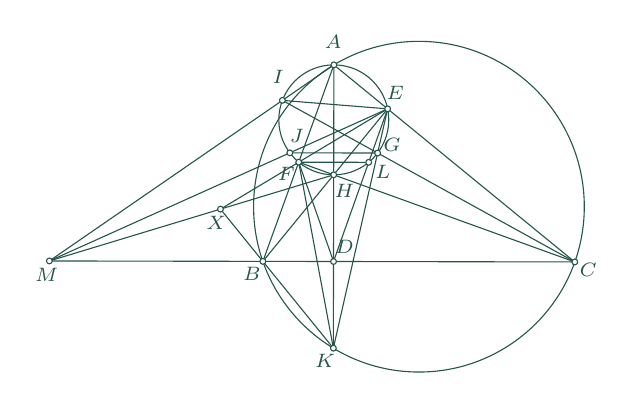
\begin{tikzpicture}[thachthuctoanhoc,scale=0.7, node font=\scriptsize]
			\draw  (2.,1.) circle (3.cm);
			\draw  (4.82748704506956,-0.0026549805211204536)-- (0.4569503366576697,3.57274128828748);
			\draw  (0.4569503366576697,3.57274128828748)-- (-0.8312527311621594,0.008028240176761736);
			\draw  (-0.8312527311621594,0.008028240176761736)-- (4.82748704506956,-0.0026549805211204536);
			\draw  (0.4569503366576697,3.57274128828748)-- (0.44724713614873457,-1.5668966757159692);
			\draw  (1.432232055433027,2.774894513168247)-- (-0.8312527311621594,0.008028240176761736);
			\draw  (1.432232055433027,2.774894513168247)-- (0.44724713614873457,-1.5668966757159692);
			\draw  (-0.18103594269847173,1.8073068848549558)-- (4.82748704506956,-0.0026549805211204536);
			\draw  (-0.18103594269847173,1.8073068848549558)-- (1.432232055433027,2.774894513168247);
			\draw  (0.45506749361137,2.5754279181153) circle (0.9973151474945761cm);
			\draw  (-0.4775862143160019,2.928690659586082)-- (4.82748704506956,-0.0026549805211204536);
			\draw  (0.4569503366576697,3.57274128828748)-- (-4.704942283062641,0.015341437467058655);
			\draw  (-4.704942283062641,0.015341437467058655)-- (-0.8312527311621594,0.008028240176761736);
			\draw  (0.45318465056507007,1.5781145479431207)-- (-4.704942283062641,0.015341437467058655);
			\draw  (-0.18103594269847173,1.8073068848549558)-- (-1.6006792850500084,0.9558492620250048);
			\draw  (-1.6006792850500084,0.9558492620250048)-- (0.44724713614873457,-1.5668966757159692);
			\draw  (1.432232055433027,2.774894513168247)-- (0.4502158933569024,0.005608936113575909);
			\draw  (-4.704942283062641,0.015341437467058655)-- (1.432232055433027,2.774894513168247);
			\draw  (-0.3426316747165554,1.9768349510073795)-- (1.2505007981656342,1.9738272520352071);
			\draw  (-0.18103594269847173,1.8073068848549558)-- (1.0882661111340752,1.8049105502452032);
			\draw  (-0.18103594269847173,1.8073068848549558)-- (0.4502158933569024,0.005608936113575909);
			\draw  (-0.18103594269847173,1.8073068848549558)-- (0.44724713614873457,-1.5668966757159692);
			\draw  (-0.4775862143160019,2.928690659586082)-- (1.432232055433027,2.774894513168247);
			\draw [fill=white] (0.4569503366576697,3.57274128828748) circle (1.5pt);
			\draw (0.44395705230662313,3.9944074949817354) node {$A$};
			\draw [fill=white] (-0.8312527311621594,0.008028240176761736) circle (1.5pt);
			\draw (-1.0309196087686856,-0.2274269473463274) node {$B$};
			\draw [fill=white] (4.82748704506956,-0.0026549805211204536) circle (1.5pt);
			\draw (5.071382576430405,-0.15368311429256215) node {$C$};
			\draw [fill=white] (0.45318465056507007,1.5781145479431207) circle (1.5pt);
			\draw (0.6467525932044781,1.284321630255861) node {$H$};
			\draw [fill=white] (0.44724713614873457,-1.5668966757159692) circle (1.5pt);
			\draw (0.2964693861990923,-1.7944833997388399) node {$K$};
			\draw [fill=white] (1.432232055433027,2.774894513168247) circle (1.5pt);
			\draw (1.5685505063765464,3.0726095818096697) node {$E$};
			\draw [fill=white] (-0.18103594269847173,1.8073068848549558) circle (1.5pt);
			\draw (-0.40409702781167944,1.5977329207343636) node {$F$};
			\draw [fill=white] (1.2505007981656342,1.9738272520352071) circle (1.5pt);
			\draw (1.5132426315862222,2.1139397521107206) node {$G$};
			\draw [fill=white] (-0.4775862143160019,2.928690659586082) circle (1.5pt);
			\draw (-0.5515846939192104,3.3491489557612892) node {$I$};
			\draw [fill=white] (-4.704942283062641,0.015341437467058655) circle (1.5pt);
			\draw (-4.754983177983841,-0.24586290560976876) node {$M$};
			\draw [fill=white] (-1.6006792850500084,0.9558492620250048) circle (1.5pt);
			\draw (-1.6761781479891333,0.7128069240891801) node {$X$};
			\draw [fill=white] (0.4502158933569024,0.005608936113575909) circle (1.5pt);
			\draw (0.6467525932044781,0.2703439257665883) node {$D$};
			\draw [fill=white] (1.0882661111340752,1.8049105502452032) circle (1.5pt);
			\draw (1.3473190072152499,1.6346048372612463) node {$L$};
			\draw [fill=white] (-0.3426316747165554,1.9768349510073795) circle (1.5pt);
			\draw (-0.21973744517726582,2.2798633764816927) node {$J$};
		\end{tikzpicture}
		\caption{\small\textit{\color{thachthuctoanhoc}Hình $1$.}}
		\vspace*{-10pt}
	\end{figure}
	Từ giả thiết về các điểm $E$, $F$, $H$ suy ra, $H$ thuộc đường tròn $(AEF)$.
	\vskip 0.05cm
	Gọi $D$ là giao điểm của các đường thẳng $AH$ và $BC$; gọi $L$, $J$ tương ứng là giao điểm thứ hai của $DE$, $ME$ và đường tròn $(AEF)$.
	\vskip 0.05cm
	Do bốn điểm $A$, $E$, $L$, $F$ cùng thuộc một đường tròn, và do bốn điểm $A$, $B$, $D$, $E$ cũng cùng thuộc một đường tròn (vì $\angle AEB = \angle ADB = {90^{\rm{o}}}$), nên
	\begin{align*}
		\left( {LF,BC} \right) &= \left( {LF,DE} \right) + \left( {DE,DB} \right) \\
		&= \left( {LF,DE} \right) + \left( {AB,AE} \right) \\
		&= 0\left( {\bmod \pi } \right).
	\end{align*}
	Suy ra, $LF \parallel BC$. \hfill ($1$)
	\vskip 0.05cm
	Do bốn điểm $A$, $E$, $I$, $H$ cùng thuộc một đường tròn, và do bốn điểm $D$, $C$, $E$, $H$ cũng cùng thuộc một đường tròn (vì $\angle HEC = \angle HDC = {90^{\rm{o}}}$), nên
	\begin{align*}
		\left( {IM,IE} \right) &= \left( {IA,IE} \right) = \left( {HA,HE} \right) \\
		&= \left( {HD,HE} \right) = \left( {CD,CE} \right) \\
		&= \left( {CM,CE} \right)\left( {\bmod \pi } \right).
	\end{align*}
	Suy ra, bốn điểm $M$, $C$, $E$, $I$ cùng thuộc một đường tròn. Vì thế
	\begin{align*}
		\left( {JG,BC} \right) &= \left( {JG,JE} \right) + \left( {JE,BC} \right) \\
		&= \left( {IG,IE} \right) + \left( {ME,MC} \right) \\
		&= \left( {IC,IE} \right) + \left( {ME,MC} \right) \\
		&= 0\left( {\bmod \pi } \right).
	\end{align*}
	Do đó, $JG \parallel BC$. \hfill ($2$)
	\vskip 0.05cm
	Từ ($1$) và ($2$), với lưu ý $DA$ là phân giác của góc $EDF$, suy ra, $L$ và $F$ đối xứng với nhau qua $DA$, $G$ và $J$ đối xứng với nhau \linebreak qua $DA$.  \hfill ($3$)
	\vskip 0.05cm
	Xảy ra hai trường hợp sau:
	\vskip 0.05cm
	$\bullet$ \textit{Trường hợp $1$: Hai đường thẳng $EF$ và $BK$ cắt nhau.} (Xem Hình $1$).
	\vskip 0.05cm
	Gọi $X$ là giao điểm của $EF$ và $KB$, ta có:
	\begin{align*}
		K(XE, HM) = &K(BE, DM) = E(BK, DM)  \\
		&\text{(do $M$, $B$, $D$ thẳng hàng)}\\
		= &E(HG, LJ) = (HG, LJ)\\
		= &(HJ, FG)  \quad\text{ (do ($3$))}\\
		= &E(HJ, FG) = E(HM, FK) \\
		= &E(XK, HM).
	\end{align*}
	Do đó, ba điểm $H$, $X$, $M$ thẳng hàng. Vì thế, ba đường thẳng $BK$, $EF$, $MH$ đồng quy.
	\vskip 0.05cm
	$\bullet$ \textit{Trường hợp $2$: $EF \parallel BK$.} (Xem Hình $2$).
	\vskip 0.1cm
	Ta nhắc lại (không chứng minh) kết quả quen biết sau:
	\vskip 0.05cm
	\textbf{\color{thachthuctoanhoc}Bổ đề.} \textit{Cho $XY$ và $ZT$ là hai tia song song. Khi đó, nếu U, V là hai điểm phân biệt, thỏa mãn
		\begin{align*}
			X(ZY, UV) = Z(XT, UV),
		\end{align*}
		thì $UV \parallel XY \parallel ZT$.}
	\vskip 0.05cm
	\begin{figure}[H]
		\vspace*{-5pt}
		\centering
		\captionsetup{labelformat= empty, justification=centering}
		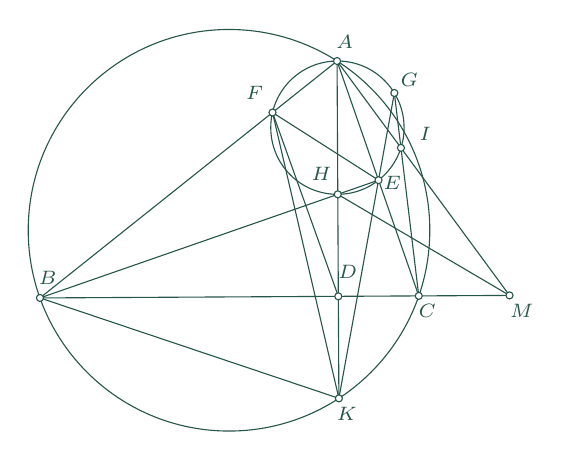
\begin{tikzpicture}[thachthuctoanhoc,scale=0.85,node font=\scriptsize]
			\draw  (1.,1.) circle (3.cm);
			\draw  (2.614310141930731,3.528636542815037)-- (-1.8244420559691163,-0.011200807195559825);
			\draw  (-1.8244420559691163,-0.011200807195559825)-- (3.83517371994642,0.019291084100292677);
			\draw  (3.83517371994642,0.019291084100292677)-- (2.614310141930731,3.528636542815037);
			\draw  (3.2336198029743386,1.748444565875232)-- (-1.8244420559691163,-0.011200807195559825);
			\draw  (1.6498826291915458,2.759520273475368)-- (3.2336198029743386,1.748444565875232);
			\draw  (2.6196759739193825,2.532681681267403) circle (0.9959693159898536cm);
			\draw  (2.614310141930731,3.528636542815037)-- (2.6414623325661375,-1.5110956594217069);
			\draw  (2.6414623325661375,-1.5110956594217069)-- (3.470229252038968,3.050865045988163);
			\draw  (3.83517371994642,0.019291084100292677)-- (3.470229252038968,3.050865045988163);
			\draw  (2.614310141930731,3.528636542815037)-- (5.190874627682908,0.026595093125835134);
			\draw  (5.190874627682908,0.026595093125835134)-- (3.83517371994642,0.019291084100292677);
			\draw  (-1.8244420559691163,-0.011200807195559825)-- (2.6414623325661375,-1.5110956594217069);
			\draw  (2.6250418059080345,1.5367268197197703)-- (5.190874627682908,0.026595093125835134);
			\draw  (1.6498826291915458,2.759520273475368)-- (2.633252069237086,0.012815580149031594);
			\draw  (1.6498826291915458,2.759520273475368)-- (2.6414623325661375,-1.5110956594217069);
			\draw [fill=white] (2.614310141930731,3.528636542815037) circle (1.5pt);
			\draw (2.727567502969913,3.8181318849538077) node {$A$};
			\draw [fill=white] (-1.8244420559691163,-0.011200807195559825) circle (1.5pt);
			\draw (-1.7074013500479646,0.2859959770145827) node {$B$};
			\draw [fill=white] (3.83517371994642,0.019291084100292677) circle (1.5pt);
			\draw (3.963023112024893,-0.20501843171239478) node {$C$};
			\draw [fill=white] (3.2336198029743386,1.748444565875232) circle (1.5pt);
			\draw (3.440330354347786,1.7115216797703234) node {$E$};
			\draw [fill=white] (1.6498826291915458,2.759520273475368) circle (1.5pt);
			\draw (1.3812376725894857,3.0578515101507455) node {$F$};
			\draw [fill=white] (2.6250418059080345,1.5367268197197703) circle (1.5pt);
			\draw (2.3791056645185082,1.8382350755708339) node {$H$};
			\draw [fill=white] (2.6414623325661375,-1.5110956594217069) circle (1.5pt);
			\draw (2.7592458519200407,-1.7504039470666048) node {$K$};
			\draw [fill=white] (3.470229252038968,3.050865045988163) circle (1.5pt);
			\draw (3.6937571459488074,3.2479216038515113) node {$G$};
			\draw [fill=white] (3.5689065068798143,2.2311584256320334) circle (1.5pt);
			\draw (3.9313447630747653,2.440123705623258) node {$I$};
			\draw [fill=white] (5.190874627682908,0.026595093125835134) circle (1.5pt);
			\draw (5.372709640305575,-0.20501843171239478) node {$M$};
			\draw [fill=white] (2.633252069237086,0.012815580149031594) circle (1.5pt);
			\draw (2.7750850263951046,0.38103102386496535) node {$D$};
		\end{tikzpicture}
		\caption{\small\textit{\color{thachthuctoanhoc}Hình $2$.}}
		\vspace*{-10pt}
	\end{figure}
	Tiếp theo, bằng cách thực hiện các biến đổi tỷ số kép tương tự như ở trường hợp $1$, ta được:
	\begin{align*}
		K\left( {BE,HM} \right) = E\left( {FK,HM} \right).
	\end{align*}
	Từ đó, do $KB \parallel EF$ nên theo Bổ đề ta có $HM \parallel KB \parallel EF$.
	\vskip 0.05cm
	Kết quả xét hai trường hợp nêu trên cho ta điều phải chứng minh theo yêu cầu đề bài.
	\vskip 0.05cm
	\textbf{\color{thachthuctoanhoc}\color{thachthuctoanhoc}Bình luận và Nhận xét}
	\vskip 0.05cm
	$\pmb{1.}$ Ở lời giải trên, ta hoàn toàn không sử dụng giả thiết ``$K$ là giao điểm của $AH$ và đường tròn $(O)$". Điều này cho thấy, kết luận của bài toán vẫn đúng, khi $K$ là một điểm tùy ý, không trùng $A$, $H$, của đường thẳng $AH.$
	\vskip 0.05cm
	$\pmb{2.}$ Tạp chí đã nhận được hai lời giải từ bạn đọc. Rất tiếc, cả hai lời giải đó đều không là lời giải hoàn chỉnh, do người giải bài hoặc đã mắc lỗi ``chính tả", hoặc đã mắc lỗi chuyên môn (không xét độ dài đại số khi sử dụng định lý Menelaus đảo).
	\begin{flushright}
		\textbf{\color{thachthuctoanhoc}\color{thachthuctoanhoc}
			Trần Quang Hùng}
	\end{flushright}
\end{multicols}
	\newpage 

%	\thispagestyle{empty}
%	\begingroup 
%%	\AddToShipoutPicture*{\put(0,0){\includegraphics[width=19.3cm]{thumoi}}}
%	\centering
%	\vspace*{0cm}
%	\endgroup
%	\newpage	
%	\pagestyle{empty}
%
%	\setcounter{figure}{0}
%	\thispagestyle{hoccungpinone}
\pagestyle{hoccungpi}
\everymath{\color{hoccungpi}}
\graphicspath{{../hoccungpi/pic/}}
\blfootnote{$^{1}$\color[named]{diendantoanhoc}THPT chuyên Lê Quý Đôn, Bình Định.}
\begingroup
\AddToShipoutPicture*{\put(0,616){\includegraphics[width=19.3cm]{../bannerhoccungpi}}}
\AddToShipoutPicture*{\put(124,525){\includegraphics[scale=1]{../tieude1.pdf}}}
\centering
\endgroup

\vspace*{192pt}

\textit{\textbf{\color{hoccungpi}LTS.} Kỳ thi Bài giảng và bài viết về Toán học, lần thứ $2$, năm $2023$, do Tạp chí Pi tổ chức, với sự phối hợp của Hội Toán học, Viện Hàn lâm Khoa học và Công nghệ Việt Nam, là một diễn đàn dành cho độc giả của Pi và những người yêu Toán nói chung. Kỳ thi đã nhận được nhiều bài viết có chất lượng chuyên môn cao. Tạp chí Pi số này xin trân trọng giới thiệu cùng bạn đọc bài viết được trao giải Nhất trong hạng mục Chuyên đề Toán học.}
\begin{multicols}{2}
	Bài viết này trình bày về hai bổ đề liên quan đến mô hình hai đoạn thẳng và một vài ứng dụng trong việc tiếp cận, khai thác một số bài toán hình học phẳng.
	\vskip 0.1cm
	\textbf{\color{hoccungpi}$\pmb{1.}$ Bổ đề về hai đoạn thẳng} 
	\vskip 0.1cm
	Trong các bài toán hình học phẳng, chúng ta khá thường xuyên gặp tình huống có hai đoạn thẳng bằng nhau. Điều đó có thể gợi đến kết quả sau đây, mà chúng tôi tạm gọi là \textit{Bổ đề hai đoạn thẳng}.
	\vskip 0.1cm 
	\textbf{\color{hoccungpi}Bổ đề $\pmb{1.}$} Cho hai đoạn thẳng $AB$ và $A'B'$ trong mặt phẳng sao cho $AB$ không cùng phương với $A'B'$ và $AB=A'B'$. Khi đó tồn tại một phép quay biến $A$ thành $A'$ và $B$ thành $B'$. đồng thời cũng tồn tại một phép quay biến $A$ thành $B'$ và biến $B$ thành $A'$.
	\vskip 0.1cm
	Trước khi đi vào chứng minh, bạn đọc có thể nhận thấy rằng, bằng cách đổi vai trò của $A'$ và $B'$, ta suy ra tồn tại phép quay thứ hai biến $A$ thành $B'$ và  $B$ thành $A'$.
	\vskip 0.1cm
	\textit{Chứng minh.} Gọi $S$ là giao điểm của $AB$ và $A'B'$. Giả sử các đường trung trực của $AA'$ và $BB'$ cắt nhau tại $T$, dễ thấy hai tam giác $TAB$ và $TA'B'$ bằng nhau (c.c.c). Do đó $(BA,BT)=(B'A',B'T)\,\,\,(\bmod \pi)$, hay $(BS,BT)=(B'S,B'T)\,\,\,(\bmod \pi)$; suy ra bốn điểm $S,T,B,B'$ đồng viên. Tương tự thì bốn điểm $S,T,A,A'$ cũng đồng viên. Rõ ràng phép quay tâm $T$, góc quay $(TA,TA')=(TB,TB')$, biến  $A,B$ tương ứng thành $A',B'$. Trong trường hợp $AA'$ và $BB'$ song song thì từ giả thiết ta có hình thang cân $ABB'A'$. Lúc này $T$ trùng $S$ và ta cũng thu được kết quả như trên.
	\begin{figure}[H]
		\vspace*{-5pt}
		\centering
		\captionsetup{labelformat= empty, justification=centering}
		\includegraphics[scale=0.63]{1}
		\vspace*{-5pt}
	\end{figure}
	Chú ý rằng bổ đề trên dẫn đến kết quả sau đây.
	\vskip 0.1cm
	\textbf{\color{hoccungpi}Hệ quả.} Cho tam giác $ABC$ cố định, các điểm $M,N$ thay đổi lần lượt thuộc các cạnh $AB,AC$ sao cho $BM=CN$. Khi đó đường tròn $(AMN)$ luôn đi qua một điểm cố định khác $A$.
	\vskip 0.1cm
	\textit{Chứng minh.} Theo giả thiết ta có $BM=CN$ nên theo chứng minh của Bổ đề $1$ thì các đường tròn $(AMN)$ và $(ABC)$ cắt nhau tại $T$ (khác $A$) là giao điểm của các đường trung trực của các đoạn thẳng $MN$ và $BC$, tức là trung điểm cung $BC$ (chứa $A$) của đường tròn $(ABC)$. Mà $(ABC)$ cố định nên $T$ cố định. Vậy,  khi $M,N$ thay đổi thì đường tròn $(AMN)$ luôn đi qua một điểm cố định $T$ (khác $A$).	\vskip 0.1cm
	\vskip 0.1cm
	Bổ đề $1$ có một mở rộng tự nhiên như sau, trong đó giả thiết bằng nhau của các đoạn thẳng được bỏ đi và phép quay được thay bằng phép vị tự quay. Vì lý do này, chúng tôi cũng gọi kết quả sau là \textit{Bổ đề hai đoạn thẳng}.
	\vskip 0.1cm
	\textbf{\color{hoccungpi}Bổ đề $\pmb{2}$.} Cho hai đoạn thẳng $AB$ và $A'B'$ trong mặt phẳng sao cho hai đường thẳng $AB$ và $A'B'$ cắt nhau tại $P$. Khi đó tồn tại một phép vị tự quay biến $A$ thành $A'$ và $B$ thành $B'$. Ngoài ra, tâm của phép vị tự quay này là giao điểm thứ hai của hai đường tròn $(PAA')$ và $(PBB')$.
	\vskip 0.1cm
	Tương tự, bằng cách hoán đổi vai trò của các điểm, dễ thấy rằng cũng tồn tại một phép vị tự quay biến $A$ thành $B'$ và $B$ thành $A'$ (tâm của phép vị tự quay này là giao điểm thứ hai của các đường tròn $(PAB')$ và $(PBA')$).
	\begin{figure}[H]
		\vspace*{-5pt}
		\centering
		\captionsetup{labelformat= empty, justification=centering}
		\includegraphics[width=1\linewidth]{2}
		\vspace*{-20pt}
	\end{figure}
	\textit{Chứng minh.} Gọi $S$ là giao điểm thứ hai của các đường tròn $(PAA')$ và $(PBB')$. Ta có $(AS,AP)=(A'S,A'P) (\bmod  \pi)$, $(BS,BP)=(B'S,B'P)(\bmod  \pi)$ nên hai tam giác $SAB$ và $SA'B'$ đồng dạng. Như vậy, $S$ là tâm của phép vị tự quay biến đoạn $AB$ thành đoạn $A'B'$. 
	\vskip 0.1cm
	\textbf{\color{hoccungpi}Nhận xét.}  Ta có một số quan sát sau:
	\vskip 0.1cm
	$1)$ Nếu $S$ là tâm phép vị tự quay biến đoạn $AB$ thành đoạn $A'B'$ thì dễ thấy hai tam giác $SAB$ và $SA'B'$ đồng dạng nên $S$ cũng là tâm của phép vị tự quay biến đoạn $AA'$ thành đoạn $BB'$.
	\vskip 0.1cm 
	$2)$ Nếu hai đường tròn $(PAA')$, $(PBB')$  có tâm lần lượt là $O$, $O'$ thì $S$ cũng là tâm của phép vị tự quay biến đường tròn $(O)$ thành đường tròn $(O')$. Do đó ta có các tam giác $SAB,SA'B'$ và $SOO'$ đồng dạng.
	\vskip 0.1cm
	$3)$ Nếu $AA'$ cắt $BB'$ tại $Q$ thì các điểm $Q,S,A,B$ đồng viên và các điểm $Q,S,A',B'$ đồng viên. Điểm $S$ chính là điểm Miquel của tứ giác toàn phần xác định bởi $ABB'A'$.
	\begin{figure}[H]
		\vspace*{-5pt}
		\centering
		\captionsetup{labelformat= empty, justification=centering}
		\includegraphics[scale=0.75]{3}
		\vspace*{-10pt}
	\end{figure}
	$4)$ Với hai đoạn thẳng $AB,A'B'$ không cùng phương, luôn có hai phép vị tự quay biến đoạn thẳng này thành đoạn thẳng kia.
	\vskip 0.1cm
	$5)$ Trong trường hợp đặc biệt khi $AB=A'B'$, ta thu lại được kết quả của Bổ đề $1$ ở trên.
	\vskip 0.1cm
	\textbf{\color{hoccungpi}$2.$  Một số áp dụng}
	\vskip 0.1cm
	Bổ đề $1$ và $2$ tỏ ra khá hữu ích trong một số tình huống. Trong bài viết này, chúng tôi xin giới thiệu ứng dụng của chúng trong việc chứng minh các đoạn thẳng bằng nhau, chỉ ra một đường thẳng hoặc đường tròn đi qua điểm cố định và chứng minh một số đường tròn đồng quy.
	\vskip 0.1cm
	$\pmb{2.1.}$ \textbf{\color{hoccungpi}Chứng minh hai đoạn thẳng bằng nhau}
	\vskip 0.1cm
	Ví dụ đầu tiên được lấy từ một bài toán Vô địch Liên bang Nga năm $2006$.
	\vskip 0.1cm
	\textbf{\color{hoccungpi}Ví dụ $\pmb{1.}$} Cho tam giác $ABC$ nội tiếp đường tròn $(O)$. Hai điểm $M,N$ thay đổi trên $AB,AC$ sao cho $MN \parallel BC$, $MN$ cắt $(O)$ tại  $P,Q$ ($M$ nằm giữa $P$ và $N$). Gọi $J,K$ tương ứng là tâm đường tròn nội tiếp các tam giác $APB$, $AQC$ và $T$ là trung điểm của cung $BC$ chứa $A$ của đường tròn $(O)$. Chứng minh rằng $TJ=TK$.
	\begin{figure}[H]
		\vspace*{-5pt}
		\centering
		\captionsetup{labelformat= empty, justification=centering}
		\includegraphics[width= 0.9\linewidth]{4}
		\vspace*{-10pt}
	\end{figure}
	\textit{Phân tích:} Đề bài xuất hiện mô hình trung điểm cung $T$ và yêu cầu chứng minh $TJ=TK$. Đây là dấu hiệu khá rõ để ta vận dụng kết quả của Bổ đề $1$. Ta cần tìm ra hai đoạn thẳng bằng nhau có các đầu mút là $J$, $K$. Để ý tới giả thiết $MN$ song song với $BC$ và tính chất của tâm đường tròn nội tiếp là ta có thể tiếp cận được bài toán.
	\vskip 0.1cm
	\textit{Lời giải.} Giả sử $AJ,AK$ cắt $(ABC)$ tương ứng tại $X$, $Y$. Dễ thấy $X$, $Y$ tương ứng là trung điểm của các cung $PB$, $QC$ của đường tròn $(ABC)$. Theo một kết quả quen thuộc thì $XB=XP=XJ$ và  $YC=YQ=YK$. Mà $YC=XB$ nên $KY=XJ$. Áp dụng Bổ đề $1$ cho tam giác $AXY$, với hai điểm $J,K$ thỏa $XJ=YK$, ta suy ra đường trung trực của đoạn thẳng $JK$ đi qua trung điểm $T$ của cung $BC$ chứa $A$ của đường tròn $(ABC)$. Vậy $TJ=TK$.
	\vskip 0.1cm
	Ví dụ sau đây, được lấy từ kỳ thi Vô địch Liên bang Nga năm $2014$, cũng có thể được giải quyết bằng cách tương tự.
	\vskip 0.1cm
	\textbf{\color{hoccungpi}Ví dụ $\pmb{2.}$} Cho tam giác $ABC$ có $AB > AC$. Các điểm $M,N$ tương ứng nằm trên các cạnh $AC,AB$ sao cho $BN=CM$. Đường thẳng $MN$ cắt $BC$ tại $P$. Gọi $I$ là tâm đường tròn nội tiếp tam giác $PNB$, $J$ là tâm đường tròn bàng tiếp góc $P$ của tam giác $PMC$ và $T$ là trung điểm cung $BC$ chứa $A$. Chứng minh rằng  $TI=TJ$.
	\vskip 0.1cm
	\textit{Phân tích:} Đề bài tiếp tục xuất hiện mô hình trung điểm cung $T$ và hai đoạn thẳng $BN,CM$ bằng nhau nên cũng gợi ý đến việc vận dụng Bổ đề $1$. Tuy nhiên ý tưởng chứng minh $TI=TJ$ không giống như lời giải của ví dụ ở trên mà phải dùng đến một phép quay phù hợp. với tâm là trung điểm $T$ của cung $BC$ chứa $A$.
	\begin{figure}[H]
		\vspace*{-5pt}
		\centering
		\captionsetup{labelformat= empty, justification=centering}
		\includegraphics[width= 1\linewidth]{5}
		\vspace*{-10pt}
	\end{figure}
	\textit{Lời giải.} Theo Bổ đề $1$ thì tồn tại phép quay tâm $T$ biến $B,\,N$ lần lượt thành $C,\,M$, do đó tam giác $TNB$ biến thành tam giác $TMC$, đường tròn $(TNB)$ biến thành đường tròn $(TMC)$ suy ra $H$ biến thành $K$ ($H, K$ lần lượt là trung điểm cung $BN,CM$). Dễ chứng minh được $HB=HN=HI$; $KC=KM=KJ$. Mà $BN=CM$ nên ta có $HI=KJ$, từ đó suy ra được $TI=TJ$.
	\vskip 0.1cm
	\textbf{\color{hoccungpi}Ví dụ $\pmb{3.}$} Cho tứ giác lồi $ABCD$ có hai đường chéo $AC$ và $BD$ cắt nhau tại $P$. Gọi $I,J$ lần lượt là tâm các đường tròn $(PAD)$, $(PBC)$. Gọi $M,N,O$ lần lượt là trung điểm các đoạn thẳng $AC,BD,IJ$. Chứng minh $OM=ON$.
	\begin{figure}[H]
		\vspace*{-5pt}
		\centering
		\captionsetup{labelformat= empty, justification=centering}
		\includegraphics[width= 1\linewidth]{6}
		\vspace*{-15pt}
	\end{figure}
	\textit{Phân tích.} Bài toán xuất hiện mô hình hai đoạn thẳng cắt nhau: $AC$ và $BD$ cắt nhau tại $P$; ngoài ra, hai đường tròn $(PAD)$ và $(PBC)$ cắt nhau tại điểm thứ hai là $Q$ nên chúng là các dấu hiệu để áp dụng Bổ đề $2$ trong việc tiếp cận bài toán. Điểm $Q$ chính là tâm của phép vị tự quay mà ta quan tâm.
	\begin{figure}[H]
		\vspace*{-10pt}
		\centering
		\captionsetup{labelformat= empty, justification=centering}
		\includegraphics[width= 0.9\linewidth]{7}
		\vspace*{-10pt}
	\end{figure}
	\textit{Lời giải.} Áp dụng Bổ đề $2$ cho hai đoạn thẳng $AC$ và $BD$, do chúng cắt nhau tại $P$, ta biết rằng tồn tại phép vị tự quay $f$ với tâm $Q$ là giao điểm thứ hai (khác $P$) của các đường tròn $(PAD)$ và $(PBC)$. Phép vị tự quay $f$ biến $A$ thành $C$, biến $D$ thành $B$. Ngoài ra, ta biết rằng cũng tồn tại phép vị tự quay $g$ với tâm là $Q$ biến $A$ thành $D$, biến $C$ thành $B$; do đó đoạn $AC$  biến thành đoạn $DB$, dẫn đến $g$ biến $M$ thành $N$. Như vậy, các đường tròn $(PAD)$, $(PBC)$, $(PMN)$ cùng đi qua $Q$. Vì $f$ biến $A$ thành $C,D$ thành $B$ và $I$ thành $J$ nên các tam giác $QDB,QAC,QIJ$ đồng dạng với nhau. Từ đó suy ra các tam giác $QDN,QAM$ và $QIO$ đồng dạng. Do đó tồn tại một phép vị tự quay tâm $Q$ biến $D$ thành $N$, $A$ thành $M$ và $I$ thành $O$. Khi đó $O$ chính là tâm đường tròn $(QMN)$ nên ta có $OM=ON$.
	\vskip 0.1cm
	\textit{Nhận xét.} Kết luận của bài toán vẫn còn đúng khi $A,B,C,D$ là bốn điểm bất kỳ sao cho $AC$ và $BD$ cắt nhau. 
	\vskip 0.1cm
	$\pmb{2.2.}$ \textbf{\color{hoccungpi}Chứng minh tính thẳng hàng, đồng quy}
	\vskip 0.1cm
	Bài toán sau đây, được lấy từ các bài toán đề nghị thi Toán quốc tế năm $2006$, minh họa một ứng dụng khác của các Bổ đề $1$ và $2$.
	\vskip 0.1cm
	\textbf{\color{hoccungpi}Ví dụ $\pmb{4.}$} Cho ngũ giác lồi $ABCDE$ thỏa mãn $\angle BAC = \angle CAD = \angle DAE,$ $\angle CBA = \angle DCA =\angle EDA$. Gọi $P$ là giao điểm của $BD$ và $CE$. Chứng minh rằng $AP$ đi qua trung điểm của $CD$. 
	\begin{figure}[H]
		\vspace*{-5pt}
		\centering
		\captionsetup{labelformat= empty, justification=centering}
		\includegraphics[width= 1\linewidth]{9}
		\vspace*{-15pt}
	\end{figure}
	\textit{Phân tích.} Trong bài toán này, dấu hiệu nhận biết việc áp dụng Bổ đề $2$ là hai đoạn thẳng $BD$ và $CE$ cắt nhau tại $P$ và các tam giác $ABC$, $ADE$ có chung đỉnh $A$ và đồng dạng với nhau. Khi đó, giao điểm thứ hai của các đường tròn $(PBC)$ và $(PDE)$ chính là tâm của phép vị tự quay. 
	\vskip 0.1cm
	\textit{Lời giải $1$.} Một mặt, theo giả thiết thì hai tam giác $ABC$ và $ADE$ đồng dạng nên có một phép vị tự quay tâm $A$ biến $B$ thành $C$, biến $D$ thành $E$, và đoạn thẳng $BD$ biến thành đoạn thẳng $CE$. Áp dụng Bổ đề $2$ cho hai đoạn thẳng $BD$ và $CE$ ta thấy rằng phép vị tự quay này có tâm là giao điểm thứ hai của các đường tròn $(PBC)$ và $(PDE)$, vì thế $A$ là giao điểm thứ hai của $(PBC)$ và $(PDE)$.
	\vskip 0.1cm
	Mặt khác, vì các tam giác $ABC,ACD,ADE$ đồng dạng (g.g) nên ta có $\angle ABC = \angle ACD, \angle ADC = \angle AED$. Do đó $CD$ là tiếp tuyến chung của hai đường tròn $(PBC)$ và $(PDE)$. Mà hai đường tròn này có trục đẳng phương là $AP$ nên nó chia đôi $CD$.
	\vskip 0.1cm
	Để so sánh với lời giải sử dụng Bổ đề 1 trên đây, chúng tôi trình bày một lời giải thứ hai.
	\textit{Lời giải $2$.} Gọi $X$ là giao điểm của $AC$ và $BD$, $Y$ là giao điểm của $AD$ và $CE$. Theo \textit{Lời giải $1$}, tồn tại phép vị tự quay $f$ tâm $A$ biến $B,\,C,\,D$ tương ứng thành $C,\,D,\,E$. Vì thế, $f$ biến các đoạn thẳng $AC$ và $BD$ tương ứng thành $AD$ và $CE$. Suy ra giao điểm của $AC$ và $BD$ biến thành giao điểm của $AD$ và $CE$, tức là $f$ biến $X$ thành $Y$.
	\begin{figure}[H]
		\vspace*{-5pt}
		\centering
		\captionsetup{labelformat= empty, justification=centering}
		\includegraphics[width= 1\linewidth]{10}
		\vspace*{-15pt}
	\end{figure}
	Từ đó ta có
	\begin{align*}
		\dfrac{XA}{XC} = \dfrac{YA}{YD}. \tag{$*$}
	\end{align*}
	Gọi $I$ là giao điểm của $AP$ với $CD$ và áp dụng định lý Ceva cho tam giác $ACD$ với điểm đồng quy $P$, ta có
	\begin{align*}
		\frac{XA}{XC}\cdot \frac{IC}{ID}\cdot\frac{YD}{YA} = 1.
	\end{align*}
	Từ đó, kết hợp ($*$), ta suy ra $IC=ID$.
	\vskip 0.1cm
	\textit{Nhận xét.}  Lời giải $2$ không dùng đến Bổ đề về hai đoạn thẳng mà dùng đến kết quả của phép vị tự quay. Việc phát hiện ra hệ thức $(*)$ là điều không hề dễ. Theo quan sát trong thực tế dạy học của tác giả, rất ít học sinh nghĩ ra  lời giải theo hướng này. Mặt khác, sau khi biết về bổ đề hai đoạn thẳng thì đa số học sinh dễ dàng phát hiện ra dấu hiệu và áp dụng vào bài toán một cách dễ dàng.
	\vskip 0.1cm
	Bài toán sau đây được lấy từ một kỳ thi Vô địch Liên bang Nga.
	\vskip 0.1cm
	\textbf{\color{hoccungpi}Ví dụ $\pmb{5.}$} Cho tam giác nhọn $ABC$. Gọi $A_1$, $B_1$, $C_1$ tương ứng là tiếp điểm của các đường tròn bàng tiếp góc $A$ với $BC$, góc $B$ với $CA$, góc $C$ với $AB$. Các đường tròn $(AB_1C_1)$, $(BC_1A_1)$, $(CA_1B_1)$ cắt lại $(ABC)$ tại $M,N,P$. Gọi $D,E,F$ là các tiếp điểm của đường tròn nội tiếp với $BC,CA,AB$. Chứng minh rằng $MD,NE,PF$ đồng quy.
	\begin{figure}[H]
		\vspace*{-5pt}
		\centering
		\captionsetup{labelformat= empty, justification=centering}
		\includegraphics[width= 0.9\linewidth]{11}
		\vspace*{-10pt}
	\end{figure}
	\textit{Phân tích.} Bằng hình vẽ ta dễ phát hiện ra rằng $M,N,P$ tương ứng là các trung điểm cung $BC,CA,AB$ của đường tròn $(ABC)$ và đây là dấu hiệu để ta nghĩ đến cách tiếp cận bài toán dựa vào Bổ đề $1$. Như vậy ta phải tìm những cặp đoạn thẳng bằng nhau, tuy nhiên điều này không quá khó khi dựa vào tính chất tiếp tuyến và tiếp điểm của các đường tròn nội tiếp, bàng tiếp.
	\vskip 0.1cm
	\textit{Lời giải.} Dễ thấy $CB_1 =AE=AF=BC_1$. Áp dụng Bổ đề $1$ ta có $M$ là trung điểm cung $BC$ chứa $A$ của $(ABC)$; tương tự với $N,P.$ Ta dễ thấy rằng hai tam giác $DEF$ và $MNP$ có các cặp cạnh tương ứng song song (chẳng hạn $NP$ và $EF$ cùng vuông góc với phân giác trong góc $A$). Vì vậy tồn tại một phép vị tự biến $D,E,F$ tương ứng thành $M,N,P$. Vậy $MD,NE,PF$ đồng quy tại tâm vị tự của hai tam giác trên. 
	\vskip 0.1cm
	Bài toán sau đây được trích từ kỳ thi chọn học sinh giỏi quốc gia năm 2017 của Việt Nam.
	\textbf{\color{hoccungpi}Ví dụ 6.} Cho tam giác $ABC$ nhọn, không cân, nội tiếp đường tròn $(O)$. Các đường cao $BE$, $CF$ cắt nhau tại $H$, $AH$ cắt $(O)$ tại $D$  (khác $A$). Các đường thẳng $DE,DF$ cắt lại $(O)$ tương ứng  $P,Q$ (khác $D$). Đường tròn $(AEF)$ cắt $(O)$ và $AO$ tương ứng tại $R,S$ (khác $A$). Chứng minh rằng $BP$, $CQ$ và $RS$ đồng quy.
	\vskip 0.1cm
	Chúng ta sẽ giới thiệu hai lời giải, một lời giải sử dụng phép biến đổi góc và lời giải còn lại sử dụng Bổ đề $2$.
	\vskip 0.1cm
	\textit{Lời giải $1$.} Gọi $X$ là trung điểm của $EF$ và $K$ là giao điểm của $AD$ và $BC$. Dễ thấy hai tam giác $BFE$ và $KHE$ đồng dạng (g.g). Gọi $T$ là trung điểm của $HE$. Khi đó, do $X$ là trung điểm $FE$ nên ta suy ra hai tam giác $BFX$ và $KHT$ đồng dạng. Vì $K$ là trung điểm $DH$ nên tam giác $KHT$ và tam giác $DHE$ đồng dạng, dẫn đến các tam giác $BFX$ và $DHE$ là đồng dạng. Suy ra  $\angle{FBX}= \angle{HDE}$, kết hợp với  $\angle{HDE}=\angle{ADP} = \angle{ABP}=\angle{FBP} $ ta được  $\angle{FBX}= \angle{FBP}.$ Từ đây ta có $B,P,X$ thẳng hàng. Tương tự ta có $C,X,Q$ thẳng hàng.
	\begin{figure}[H]
		\vspace*{-10pt}
		\centering
		\captionsetup{labelformat= empty, justification=centering}
		\includegraphics[width= 0.9\linewidth]{12}
		\vspace*{-15pt}
	\end{figure}
	Kẻ đường kính $AL$ của $(O)$. Dễ thấy $SH$ đi qua $L$ và do tứ giác $HBLC$ là hình bình hành nên $HL$ đi qua trung điểm $M$ của $BC$. Dễ thấy hai tam giác $SEC$ và $SFB$ đồng dạng (g.g) nên hai tam giác $SEF$ và $SCB$ đồng dạng (c.g.c). Mà hai tam giác này có các trung tuyến tương ứng là $SX$ và $SM$ nên ta suy ra $\angle FSX =  \angle BSM$. Tương tự, do hai tam giác $SFB$ và $SRL$ đồng dạng (g.g) nên hai tam giác $SFR$ và $SBL$ đồng dạng (c.g.c), dẫn đến  $\angle FSR=\angle BSL=\angle BSM=\angle FSX$. Từ đó suy ra $S,X,R$ thẳng hàng. Vậy, $SR,BP,CQ$ đồng quy tại trung điểm $X$ của $EF$.
	\vskip 0.1cm
	\textit{Lời giải $2$.} Gọi $X$ là trung điểm của $EF$. Tương tự như \textit{Lời giải $1$}, ta cũng chứng minh được $BP$ và $CQ$ đi qua $X$. Ta cần chứng minh $SR$ cũng đi qua $X$. Kẻ đường kính $AL$. Áp dụng Bổ đề $2$ cho hai đoạn thẳng $BF$ và $CE$ (và để ý rằng chúng cắt nhau tại $A$) ta suy ra $S$ là tâm của phép vị tự quay $f$ biến đoạn $FE$ thành đoạn $BC$ và biến $X$ biến thành $M$. Từ đó $f$ biến $(AEF)$ thành $(ABC)$. Kết hợp với việc $A,R,L$ thẳng hàng, ta suy ra $f$ biến $R$ thành $L$. Các điểm $S,L,M$ tương ứng biến thành $S,R,X$. Mà  $S,L,M$ thẳng hàng nên $S,R,X$ thẳng hàng. Vậy, $SR,BP,CQ$ đồng quy tại $X$.
	\vskip 0.1cm
	\textit{Nhận xét.} Ở lời giải thứ nhất, để chứng minh $SR$ đi qua $X$, ta đã sử dụng phép biến đổi góc dựa vào việc tìm ra những cặp tam giác đồng dạng khá phức tạp. Tuy nhiên ở lời giải thứ hai thì việc áp dụng Bổ đề $2$ cho ta cách tiếp cận dễ dàng hơn nhiều. Dấu hiệu nhận biết ở đây là việc hai đường tròn $(O)$ và $(AEF)$ cắt nhau tại $ A,S$ và có $BF$ cắt $CE$ tại $A$.
	\vskip 0.1cm 
	$\pmb{2.3.}$ \textbf{\color{hoccungpi} Chứng minh đường thẳng hoặc đường tròn luôn qua điểm cố định}
	\vskip 0.1cm
	Bài toán sau đây được lấy từ đề thi Toán quốc tế (IMO) năm $2005$.
	\vskip 0.1cm
	\textbf{\color{hoccungpi}Ví dụ $\pmb{7}$.} Cho $ABCD$ là tứ giác lồi có $AD=BC$ và $AD,BC$ không song song. Gọi $E,F$ tương ứng  là các điểm trên $BC,AD$ sao cho $BE=DF$. Các đường thẳng  $AC$ và $BD$ cắt nhau tại $P$, các đường thẳng $BD$ và $EF$ cắt nhau tại $Q$, các đường thẳng $EF$ và $AC$ cắt nhau tại $R$. Chứng minh rằng, khi $E$ và $F$ thay đổi, đường tròn $(PQR)$ đi qua một điểm cố định khác $P$.
	\begin{figure}[H]
		\vspace*{-5pt}
		\centering
		\captionsetup{labelformat= empty, justification=centering}
		\includegraphics[width= 1.02\linewidth]{14}
		\vspace*{-15pt}
	\end{figure}
	\textit{Lời giải $1$.} Theo Bổ đề $1$, áp dụng cho hai đoạn thẳng $AD=BC$ có $AC$ cắt $BD$ tại $P$,  ta có giao điểm $S$ của hai đường tròn $(PAD)$ và $(PBC)$ là tâm phép quay (góc  $ \angle BSD$) biến $A$ thành $C$ và biến $D$ thành $B$, do đó ta có các tam giác cân $SAC,SBD$ đồng dạng. Vì $FD/FA=EB/EC$ nên phép quay này biến $F$ thành $E$, do đó ta có $SF=SE$ và $(FS, FR)=(FS, FE)=(AS, AC)=(AS, AR)\,\,\,(\bmod \pi)$. Do đó $A,S, R, F$ đồng viên. Tương tự, $B, E, Q, S$ đồng viên và $D, F, S, Q$ đồng viên. Từ đó $(RS, RP)=(FS, FA)=(FS, FD)=(QS, QP)\,\,\,(\bmod \pi)$. Suy ra $(PQR)$ đi qua điểm $S$ cố định.
	\vskip 0.1cm
	\textit{Lời giải $2$.} Theo Bổ đề $2$, tồn tại phép vị tự quay $f$ biến $A$ thành $C$ và biến $D$ thành $B$. Khi đó $f$ biến $ F$ thành $E$ (do $FD/FA=EB/EC$), và đoạn $DF$ biến thành đoạn $BE$. Do đó hai tứ giác $ACBD$ và $EFDB$ có chung điểm Miquel. Tâm của phép vị tự quay $f$ là giao điểm thứ hai $S$ của hai đường tròn $(PAD)$ và $(PCB)$, cũng là điểm Miquel chung của các tứ giác toàn phần $ACBD$ và $EFDB$. Do đó $S$ thuộc các đường tròn $(QEB)$ và $(QFD)$. Dễ thấy $S$ cũng là điểm Miquel chung của các tứ giác toàn phần $DFRP$ và $CEQP$, do đó $S$ thuộc $(PQR)$. Vì các đường tròn $(PAD)$ và $(PBC)$ cố định nên $S$ cố định. Vậy, đường tròn $(PQR)$ luôn đi qua điểm $S$ cố định. 
	\begin{figure}[H]
		%		\vspace*{-5pt}
		\centering
		\captionsetup{labelformat= empty, justification=centering}
		\includegraphics[width= 1\linewidth]{15}
		\vspace*{-10pt}
	\end{figure}
	\textit{Nhận xét.} $1)$ Điều thú vị là đối với bài toán này lại, chúng ta vừa có thể áp dụng Bổ đề $1$, vừa có thể áp dụng Bổ đề $2$ để giải. Điều đó cho thấy sự đa dạng và phạm vi vận dụng rộng rãi của hai bổ đề mà chúng ta đã đề cập. Trong bài toán trên, dấu hiệu để phát hiện và tiếp cận theo hướng Bổ đề $1$  là sự xuất hiện của hai đoạn thẳng bằng nhau. Mặt khác, dấu hiệu để tiếp cận và vận dụng bổ đề $2$ là có mô hình hai đoạn thẳng $AC$ và $BD$ cắt nhau tại $P$, đồng thời hai đường tròn $(PAD)$, $(PBC)$ cắt nhau tại $P$ và $S$. Hơn nữa, bài toán cũng xuất hiện hai điểm $E,F$ chia các đoạn thẳng với tỷ lệ bằng nhau nên ta nghĩ đến phép vị tự quay biến $F$ thành $E$; tâm của phép vị tự quay chính là điểm $S$.
	\vskip 0.1cm
	$2)$ Nếu thay giả thiết tứ giác $ABCD$ lồi thành bốn điểm $A, B, C, D$ bất kỳ ta vẫn thu được kết luận tương tự và các lời giải trên vẫn còn đúng.
	\vskip 0.1cm
	\textbf{\color{hoccungpi}Ví dụ $\pmb{8.}$} Cho tam giác $ABC$ nội tiếp đường tròn $(O)$ cố định với $B,C$ là các điểm cố định và điểm $A$ thay đổi trên $(O)$. Các đường cao $AD,BE,CF$ đồng quy tại $H,BO$ và $CO$ tương ứng cắt $DF,DE$ tại $K,L,KL$ cắt $EF$ tại $P$. Chứng minh rằng đường tròn $(PEL)$ luôn qua một điểm cố định.
	\vskip 0.1cm
	\textit{Phân tích.} Để ý rằng các điểm $E,F,K,L$ cùng với $P,D$ lập thành một tứ giác toàn phần, vì vậy khi xét điểm cố định mà đường tròn $(EPL)$ đi qua, ta quan tâm đến điểm Miquel của tứ giác toàn phần $EFKLPD$. Lại có $(EFD)$ chính là đường tròn Euler của tam giác $ABC$, và trung điểm $M$ của $BC$ là trung điểm cung $EF$ chứa $D$ của đường tròn này. Như vậy, ta chỉ cần chứng minh $M$ chính là điểm Miquel của tứ giác toàn phần đã nêu. Để chỉ ra điều đó, ta đưa về mô hình hai đoạn thẳng bằng nhau và áp dụng Bổ đề $1$. Từ đó ta có thể tiếp cận bài toán như sau.
	\begin{figure}[H]
		\vspace*{-5pt}
		\centering
		\captionsetup{labelformat= empty, justification=centering}
		\includegraphics[width= 1\linewidth]{16}
		\vspace*{-10pt}
	\end{figure}
	\textit{Lời giải.} Vì $BH, BO$ đẳng giác trong góc $B$ nên $BO$ vuông góc với $FD$. Tương tự, $CO$ vuông góc với $ED$. Để ý rằng $B,C$ tương ứng là tâm các đường tròn bàng tiếp góc $E,F$ của tam giác $DEF$ nên ta dễ chứng minh được $KF=LE$. Gọi $M$ là trung điểm $BC$. Dễ thấy $ME=MF$ nên $M$ là trung điểm của cung $FE$ chứa $D$ của đường tròn $(FDE)$, đường tròn Euler của tam giác $ABC$. Do đó theo Bổ đề $1$ thì $M$ là điểm Miquel của tứ giác toàn phần $EFKLDP$. Vì thế đường tròn $(LEP)$ luôn qua điểm $M$ cố định khi $A$ di động trên $O$.
	\vskip 0.1cm
	Bài toán sau đây do tác giả Trần Quang Hùng đề xuất.
	\vskip 0.1cm
	\textbf{\color{hoccungpi}Ví dụ $\pmb{9.}$} Cho tam giác $ABC$. Các điểm $E,F$ tương ứng thay đổi trên $AC,AB$ sao cho $CE=BF$. Chứng minh rằng đường thẳng Euler của tam giác $AEF$ luôn đi qua một điểm cố định.
	\vskip 0.1cm
	\textit{Phân tích.} Rõ ràng bài toán này có mô hình hai đoạn thẳng bằng nhau là $CE=BF$ nên ta có thể vận dụng Bổ đề $1$ để tiếp cận. Theo Bổ đề $1$ thì hai đường tròn $(AEF)$ và $(ABC)$ cắt nhau tại trung điểm cung của mỗi đường tròn, từ đó ta có thêm thông tin để giải bài toán.
	\vskip 0.1cm
	\textit{Lời giải.} Gọi $ G,L$ tương ứng là trọng tâm các tam giác $ABC,AEF$. Gọi $(O)$ và $(K)$ tương ứng là các đường tròn ngoại tiếp các tam giác $ABC, AEF$. Khi đó $LK,GO$ tương ứng là đường thẳng Euler của các tam giác $AEF,ABC$. Gọi giao điểm của $LK$ và $ GO$ là $R$. Ta sẽ chứng minh $R$ là một điểm cố định. Thật vậy, theo Bổ đề $1$ thì $(O)$ và $(K)$ cắt nhau tại $T$ trên các đường trung trực $EF,BC$. Gọi $ M,N$ tương ứng là trung điểm của các đoạn thẳng $BC,EF$. Ta thấy rằng các tam giác cân $TEF,TBC$ đồng dạng, do đó ta suy ra được $\dfrac{TK}{TN} = \dfrac{KO}{MN} = \dfrac{TO}{TM}$, là tỷ số không đổi.
	\begin{figure}[H]
		\vspace*{-5pt}
		\centering
		\captionsetup{labelformat= empty, justification=centering}
		\includegraphics[width= 1\linewidth]{17}
		\vspace*{-10pt}
	\end{figure}
	Suy ra $MN\parallel KO$. Ta lại có $\dfrac{GL}{MN} = \dfrac{2}{3}$  và $GL\parallel MN$, do đó $GL\parallel KO$ và
	\begin{align*}
		\dfrac{GL}{KO} = \dfrac{GL}{MN}\cdot \frac{MN}{KO} = \dfrac{2}{3} \cdot \dfrac{TM}{TO}.
	\end{align*}
	Từ đó, tỷ số $\dfrac{RG}{RO} = \dfrac{GL}{KO}$ là không đổi, do đó điểm $R$ là cố định. Vậy $KL$ luôn đi qua điểm $R$ cố định.
	\vskip 0.1cm
	$\pmb{2.4.}$ \textbf{\color{hoccungpi}Chứng minh nhiều đường tròn đồng quy}
	\vskip 0.1cm
	Bài toán sau đây xuất hiện trong đề thi Olympic Toán quốc gia của Mỹ năm $2006$.
	\vskip 0.1cm
	\textbf{\color{hoccungpi}Ví dụ $\pmb{10.}$}  Cho tứ giác lồi $ABCD$ có các cặp cạnh đối không song song và $E,F$ lần lượt là các điểm trên các cạnh $AD$ và $BC$ sao cho  $\dfrac{AE}{ED} = \dfrac{BF}{FC}$, $EF$ cắt $AB,CD$ lần lượt tại $S,T$. Chứng minh các đường tròn $(SAE)$, $(SBF)$, $(TCF)$, $(TDE)$ cùng đi qua một điểm.
	\vskip 0.1cm
	\textit{Phân tích.} Đề bài cho tứ giác toàn phần $ABCD$ và các điểm $E,F$ lần lượt chia các đoạn $AD,BC$ theo cùng tỷ số nên ta có thể liên tưởng đến mô hình hai đoạn thẳng. Hơn nữa, yêu cầu bài toán là chứng minh các đường tròn đồng quy nên ta có thể nghĩ đến điểm Miquel của tứ giác toàn phần, cũng chính là tâm của phép vị tự quay trong Bổ đề $2$.
	\begin{figure}[H]
		\vspace*{-5pt}
		\centering
		\captionsetup{labelformat= empty, justification=centering}
		\includegraphics[width= 1\linewidth]{18}
		\vspace*{-10pt}
	\end{figure}
	\textit{Lời giải.} Gọi $M$ là tâm của phép vị tự quay $f$ biến $A$ thành $B$, biến $D$ thành $C$, do đó biến $AD$ thành $BC$. Vì các điểm $E,F$ chia các đoạn thẳng này theo cùng tỷ số nên phép vị tự quay này cũng biến $E$ thành $F$. Do đó $f$ biến $AE$ thành $BF$ và biến $ED$ thành $FC$. Như vậy, tâm $M$ là điểm Miquel chung của các tứ giác toàn phần $ABFE$ và $EFCD$ (cũng như tứ giác $ABCD$). Vậy, các đường tròn $(SAE)$, $(SBF)$, $(TCF)$, $(TDE)$ cùng đi qua điểm Miquel $M$.
	\begin{figure}[H]
		%		\vspace*{-5pt}
		\centering
		\captionsetup{labelformat= empty, justification=centering}
		\includegraphics[width= 1\linewidth]{19}
		\vspace*{-10pt}
	\end{figure}
	\textit{Nhận xét:} Nếu thay giả thiết tứ giác $ABCD$ lồi bởi bốn điểm $A,B,C,D$ bất kỳ thì ta cũng thu được kết quả tương tự.
	\vskip 0.1cm
	$\pmb{2.5.}$ \textbf{\color{hoccungpi}Một số bài tập}
	\vskip 0.1cm
	Để kết thúc bài viết, chúng tôi xin mời độc giả thử sức mình với một số bài toán mà lời giải có thể sử dụng các Bổ đề $1$ và $2$.
	\vskip 0.1cm
	\textbf{\color{hoccungpi}Bài $\pmb{1}$ (Chọn đội tuyển Mỹ năm $\pmb{2007}$).} Hai đường tròn $(O)$ và $(O')$ cắt nhau tại $P,Q$.  Qua $P$ vẽ hai cát tuyến $PAB$ và $PCD$ sao cho $A,C$ thuộc $(O)$ và $B,D$ thuộc $(O')$. Tia $BD$ cắt đoạn $AC$ tại $X$. Lấy điểm $Y$ thuộc $(O)$ và $Z$ thuộc $(O')$ sao cho $PY\parallel BD,PZ\parallel AC$. Chứng minh $Q,X,Y,Z$ thẳng hàng.
	\vskip 0.1cm
	\textbf{\color{hoccungpi}Bài $\pmb{2}$.} Cho tam giác $ABC$, các điểm $E,F$ di chuyển trên $AC,AB$ sao cho $CE=BF$. Chứng minh rằng tâm đường tròn Euler của tam giác $AEF$ luôn thuộc một đường thẳng cố định khi $E,F$ di chuyển.
	\vskip 0.1cm
	\textbf{\color{hoccungpi}Bài $\pmb{3}$.} Cho tam giác $ABC$ có trung tuyến $AM$. Gọi $I,J$ lần lượt là tâm các đường tròn $(AMB),(AMC),O$ là tâm đường tròn $(ABC)$. Chứng minh $AO$ là đường đối trung của tam giác $AIJ$.
	\vskip 0.1cm
	\textbf{\color{hoccungpi}Bài $\pmb{4}$ (Olympic Iran $\pmb{1997}$).} Cho tam giác ABC nội tiếp đường tròn $(O)$. Điểm $P$ di chuyển trên cung $BC$ không chứa $A$, gọi $I,J$ lần lượt là tâm nội tiếp các tam giác $APB,APC$. Chứng minh đường tròn $(PIJ)$ luôn đi qua một điểm cố định.
	\vskip 0.1cm
	\textbf{\color{hoccungpi}Bài $\pmb{5}$.} Cho hai đường tròn $(O)$ và $(O')$ cắt nhau  tại $A,B$. Một cát tuyến thay đổi qua $A$ cắt $(O),(O')$ lần lượt tại $D,E$. Tiếp tuyến của $(O)$ tại $D$ và tiếp tuyến của $(O')$ tại $E$ cắt nhau tại $P$. Chứng minh rằng trung trực của đoạn $BP$ luôn tiếp xúc với một đường tròn cố định.
	\vskip 0.1cm
	\textbf{\color{hoccungpi}Bài $\pmb{6}$ (Olympic Canada $\pmb{2013}$).} Cho tam giác $ABC$ vuông tại $C$ có trọng tâm $G$, gọi $P$ là điểm trên $AG$ sao cho  $\angle CPA = \angle CAB$, $Q$ là điểm trên $BG$ sao cho  $\angle CQB = \angle ABC$. Chứng minh rằng các đường tròn $(AQG)$ và $(BPG)$ cắt nhau tại một điểm thuộc cạnh $AB$.
	\vskip 0.1cm
	\textbf{\color{hoccungpi}Bài $\pmb{7}$.} Cho tam giác $ABC$ nhọn có trực tâm $H$ và nội tiếp đường tròn $(O)$. Trung trực $AH$ cắt $AB,AC$ lần lượt tại $D,E$. Chứng minh rằng $OA$ là phân giác của góc  $\angle DOE$.
	\vskip 0.1cm
	\textbf{\color{hoccungpi}Bài $\pmb{8}$ (Olympic Trung Quốc $\pmb{1992}$).} Cho tứ giác lồi $ABCD$ nội tiếp đường tròn $(O),AC$ cắt $BD$ tại $P$, các đường tròn $(PAB)$ và $(PCD)$ cắt nhau tại $Q$ khác $P$ và $O$. Chứng minh $QO$ vuông góc với $QP$.
	\vskip 0.1cm
	\textbf{\color{hoccungpi}Bài $\pmb{9}$ (Olympic Toán quốc tế $\pmb{2004}$).} Cho tứ giác lồi $ABCD$, đường chéo $BD$ không là phân giác các góc  $\angle ABC, \angle CDA$. Điểm $P$ nằm trong tứ giác sao cho  $\angle PBC = \angle DBA, \angle DBC = \angle BDA$. Chứng minh tứ giác $ABCD$ nội tiếp được khi và chỉ khi $PA=PC$.
	\vskip 0.1cm
	\textbf{\color{hoccungpi}Bài $\pmb{10}$.} Cho tam giác $ABC$ nội tiếp đường tròn $(O),N$ là trung điểm cung $BC$ chứa $A$ của $(O), M$ là một điểm bất kỳ trên trung trực đoạn $BC$. Gọi $I,J$ lần lượt là tâm đường tròn bàng tiếp góc $A$ của các tam giác $ABM,ACM$. Chứng minh $I,J,A,N$ đồng viên.
	\vskip 0.1cm
	\textbf{\color{hoccungpi}Tài liệu tham khảo}
	\vskip 0.1cm
	[$1$] Lê Bá Khánh Trình, \textit{Hình học tĩnh và động}, tạp chí Pi, số $8$, tháng $8/2019$. 
	\vskip 0.1cm
	[$2$] Trần Quang Hùng. \textit{Ứng dụng một số bổ quen thuộc vào các bài toán hình học thi Olympic}.
	\vskip 0.1cm
	[$3$] Nguyễn Minh Hà, Nguyễn Xuân Bình, \textit{Bài tập nâng cao và một số chuyên đề Hình học $10$}, NXB Giáo dục, $2008$.
	\vskip 0.1cm
	[$4$] Nguyễn Văn Ban, Hoàng Chúng, \textit{Hình học của tam giác}, NXB Giáo dục.
	\vskip 0.1cm
	[$5$] V.V. Praxolov, \textit{Các bài toán về hình học phẳng, Tập II}, NXB Hải Phòng, $2002$.
	\vskip 0.1cm
	[$6$] Johnson, A. R, \textit{Advanced Euclidean Geometry}, Publications, Inc, Mineola, New York, $2007$.
\end{multicols}


%	\newpage
%
%	\setcounter{figure}{0}
%	\thispagestyle{cackithitoannone}
\pagestyle{cackithitoan}
\everymath{\color{cackithi}}
\graphicspath{{../cackithi/pic/}}
\begingroup
\AddToShipoutPicture*{\put(0,616){\includegraphics[width=19.3cm]{../bannercackithi}}}
\AddToShipoutPicture*{\put(45,530){\includegraphics[scale=0.95]{../tieude.pdf}}}
\centering
\endgroup
\vspace*{175pt}

\begin{multicols}{2}
	Kỳ thi chọn học sinh giỏi quốc gia môn Toán THPT năm học $2022-2023$ được diễn ra trong hai ngày $24$ và $25/2/2023$ với xấp xỉ $500$ thí sinh tham gia dự thi. Kết quả kỳ thi được công bố vào chiều tối ngày $13/3/2023$. Trong bài viết này, chúng tôi xin đưa ra một số tổng kết, đánh giá và bình luận về đề thi và kết quả của kỳ thi năm nay.
	\vskip 0.05cm
	\textbf{\color{cackithi}Về đề thi}
	\vskip 0.05cm
	Đề thi năm nay vẫn giữ ổn định cấu trúc đề thi HSG quốc gia môn toán từ gần $15$ năm nay.
	Ngày thứ nhất bốn bài toán lần lượt thuộc các phân môn: giải tích, số học, đại số và hình học. Bài toán giải tích là một bài toán thuộc chủ đề quen thuộc: giới hạn dãy số. Ý đầu ở mức căn bản sử dụng tính chất dãy đơn điệu và bị chặn thì có giới hạn, còn ý sau liên quan đến khảo sát dãy số ở dạng tích bằng cách logarit hóa. Việc sử dụng phép thế lượng giác chỉ giúp nhìn ra vấn đề nhanh hơn và giải gọn hơn chứ không phải là cách giải tiên quyết. Có thể đánh giá đây là bài dễ nhất của ngày thứ nhất cũng là bài dễ nhất của cả hai ngày. 
	\vskip 0.05cm
	Ở Bài $2$, bài số học, thì ý đầu là một ý hoàn toàn đại số và rất cơ bản, chúng ta có thể tìm được công thức tổng quát của dãy số một cách dễ dàng. Phần chính của bài toán này là ý sau (không liên quan gì đến ý đầu). Yêu cầu bài toán được phát biểu khá thú vị, thoạt nhìn thì có vẻ rất ``khủng" nhưng nếu xem kỹ về bản chất thì khá đơn giản, chỉ dùng đến nguyên lý Dirichlet và tính tuần hoàn của số dư của dãy truy hồi nguyên. 
	\vskip 0.05cm
	Bài $3$ là một bài về bất đẳng thức ba biến có điều kiện, có thể nói là có dạng khá quen thuộc. Hướng đi tự nhiên nhất của bài này là chuẩn hóa rồi đưa về một biến (cụ thể là biến $r = abc$). Như vậy, xét về độ khó thì bài $3$ nhẹ nhàng hơn Bài $2$ cả về phát biểu (rất dễ hiểu), hướng đi và kỹ thuật.  
	\vskip 0.05cm
	Bài $4$ là một bài toán hình học có hai ý gần như độc lập. Ý đầu có điểm mấu chốt là có được $AKJH$ là hình bình hành rồi dùng tứ giác nội tiếp hoặc hàng điểm điều hoàn. Ý sau dùng tính chất của đường thẳng Simson và phép vị tự sẽ làm khá gọn. 
	\vskip 0.05cm
	Đánh giá sơ bộ cho đề thi ngày $1$ là đề khá dài, có nhiều ý, đặc biệt là các ý trong các Bài $2$ và $4$ hầu như không lên quan đến nhau. Các ý khó là $2b$ và $4a$, $4b$.
	\vskip 0.05cm 
	Đề thi ngày thứ hai gồm $3$ bài toán thuộc ba phân môn, lần lượt là: đại số, tổ hợp, hình học.
	\vskip 0.05cm
	Bài $5$ là một bài phương trình hàm có dạng giống (và cách giải cũng tương tự) với một bài toán trong IMO shortlist $2000$, khai thác tính toàn ánh và đơn ánh của phương trình hàm có biến nằm ngoài biểu thức hàm số. Không khó về mặt ý tưởng nhưng đây vẫn là một thách thức lớn cho thí sinh với những khó khăn kỹ thuật.   
	\vskip 0.05cm
	Bài $6$ là một bài toán tổ hợp về họ tập con khá quen thuộc sử dụng phương pháp đếm bằng hai cách. Dạng toán này đã xuất hiện nhiều, chỉ là với các tham số khác. Có lẽ khó khăn lớn nhất trong bài này là việc xây dựng ví dụ (nhất là trong tình huống các đánh giá đưa ra mới chỉ là các điều kiện cần). Phát biểu của bài toán này cũng hơi rối rắm và có lẽ điều đó cũng làm cho số thí sinh làm tốt bài này không nhiều.
	\vskip 0.05cm
	Bài $7$ là một bài toán hình học có cấu hình khá phức tạp với ý đầu là một bất đẳng thức hình học và ý sau yêu cầu chứng minh tính chất hình học thuần túy. Ý đầu có thể giải quyết khá gọn nếu biết một bổ đề quen thuộc sau: Cho góc xAy. Đường tròn $(I)$ tiếp xúc $Ax$, $Ay$ tại $B$, $C$. Đường tròn $(J)$ qua $A$ tiếp xúc $(I)$ cắt $Ax$, $Ay$ tại $D$, $E$. Khi đó $AD + AE \ge BC$. Ý sau tuy có vẻ rối rắm nhưng lại có nhiều hướng để tiếp cận.
	\vskip 0.05cm
	So với ngày thứ nhất thì đề thi ngày thứ hai cân bằng hơn: Bài $6$ với hai ý $6a$, $6b$ khá nhẹ nhàng, Bài $5$ cũng có ý $5a$ cơ bản, còn lại các ý khó là $5b$, $6c$ và bài hình. 
	\vskip 0.05cm
	Về tổng thể đề thi năm nay được đánh giá là khó, dài với nhiều ý (hầu như bài nào cũng có ý $a$, $b$, thậm chí $c$), hơi nặng về kỹ thuật, phần hình học khá nặng với hai bài, bốn ý riêng biệt, cấu hình rất phức tạp và đều đặt ở vị trí bài cuối (và quả thật cũng là bài khó của từng ngày).
	\vskip 0.05cm
	\textbf{\color{cackithi}Về kết quả}
	\vskip 0.05cm
	Trước hết là điểm chuẩn. Dù đề thi năm nay được đánh giá là khá khó, dài và nhiều ý, nhưng điểm chuẩn không quá thấp như dự đoán ban đầu: KK -- $13{,}5$; Ba: $16{,}5$; Nhì: $20{,}5$; Nhất $28$ và điểm để dự thi chọn đội tuyển là $23$. 
	\vskip 0.05cm
	Kết quả tốt nhất thuộc về đội tuyển Hà Tĩnh với hai giải nhất, tám giải nhì. Trong đó có em Trần Minh Hoàng, học sinh lớp $10$ chuyên Hà Tĩnh đạt thủ khoa với số điểm $32$ (với một đề thi có đến năm bài ở mức khó thì đây là một kết quả tuyệt vời đối với một bạn học sinh lớp $10$).
	\vskip 0.05cm
	Tiếp theo là đội tuyển Phú Thọ với hai giải nhất, năm giải nhì, ba giải ba. Đội tuyển trường PTNK, ĐHQG--HCM vẫn giữ được phong độ với hai giải nhất, ba giải nhì, hai giải ba và hai giải KK. 
	\vskip 0.05cm
	Ngoài ba đơn vị dẫn đầu có hai giải nhất, các đơn vị có giải nhất và cũng có kết quả tốt là: ĐHKHTN, ĐQGHN: một giải nhất, ba nhì, ba giải ba; Bắc Ninh: một giải nhất, hai giải nhì, năm giải ba; Hà Nội, một giải nhất, ba giải nhì, bốn giải ba, sáu giải KK; Hải Phòng: một giải nhất, ba giải nhì, hai giải ba, hai giải KK; Thừa Thiên Huế: một giải nhất, một giải ba, bốn giải KK.
	\vskip 0.05cm
	Đây đều là các đơn vị có truyền thống của VMO. Ở một góc nhìn khác, VMO năm nay có những đơn vị có những thành tích vượt bậc so với chính mình như Sóc Trăng có một giải nhì, một giải ba, hai giải KK; Lâm Đồng có hai giải nhì, một giải ba, một giải KK; Điện Biên có hai giải ba, Trà Vinh có một giải nhì, Kiên Giang có một giải  ba, một giải KK. Đặc biệt, có hai bạn không phải là học sinh trường chuyên cũng đã xuất sắc đạt giải: một bạn học sinh THPT FPT Cần Thơ đạt giải ba và một bạn học sinh THCS \& THPT Đông Du Đăk lak đạt giải khuyến khích. 
	\vskip 0.05cm
	Cuối cùng xin được điểm qua về bản đồ TST năm nay. Với điểm chuẩn là $23$ có $48$ bạn đạt mốc điểm này, được phân bổ như sau: đông đảo nhất là Hà Tĩnh với tám bạn, tiếp đến là Phú Thọ với năm bạn. Năm đội mạnh tiếp theo, mỗi đội có ba học sinh gồm PTNK, ĐHQG--HCM; KHTN, ĐHQG--HN, ĐHSP HN, Hà Nội, Hải Phòng; các đội có hai thí sinh tham dự TST gồm Bắc Ninh, Nam Định, Nghệ An và Thanh Hóa. Cuối cùng là nhóm các đơn vị có một suất TST: Bà Rịa -- Vũng Tàu, Bắc Giang, Đà Nẵng, Hải Dương, Hưng Yên, Lâm Đồng, Quảng Bình, Quảng Ngãi, Quảng Ninh, Tp HCM, Thừa Thiên -- Huế và Trà Vinh. $48$ em này sẽ cùng với bạn Phạm Việt Hưng, HCV IMO $2022$, tranh sáu suất dự IMO $2023$ tại Nhật Bản. 
	\vskip 0.05cm
	Trong các suất dự TST chúng tôi đặc biệt muốn nhắc tới hai suất của Trà Vinh và Lâm Đồng. Với Trà Vinh, có lẽ đây là suất TST đầu tiên còn với Lâm Đồng thì điều đặc biệt là suất TST này thuộc về học sinh trường chuyên Bảo Lộc, một trường chuyên thứ hai trong tỉnh mới được thành lập sau này. Và bạn học sinh đạt giải nhì có điểm số rất cao, $27$ điểm, tức là chỉ thiếu tí chút là đạt giải nhất.
	\vskip 0.05cm
	Nói câu chuyện về các trường hợp FPT Cần Thơ, Đông Du Đak lak, Điện Biên, Kiên Giang, Sóc Trăng, Trà Vinh hay chuyên Bảo Lộc để thấy rằng ở đâu cũng có học sinh có tố chất tốt, chỉ cần có những người thầy tâm huyết, biết thổi vào học trò sự tự tin và niềm đam mê. Ở thời đại của Internet, đặc biệt với sự cởi mở của cộng đồng toán, các vấn đề về tài liệu, thông tin sẽ không còn là lợi thế của riêng ai, và, với hình thức học online, các bạn học sinh ở mọi miền đều có cơ hội được học với các thầy giáo, các chuyên gia giỏi. Cơ hội được học hỏi đồng đều hơn và cơ hội thành công cũng đồng đều hơn.
	\vskip 0.05cm
	\textbf{\color{cackithi}Một số bình luận và đề xuất}
	\vskip 0.05cm
	Trước hết là về đề thi. Với thời gian $180$ phút làm bài, đề thi như vậy là quá dài với quá nhiều ý, quá nhiều yêu cầu, đặc biệt là ở ngày thi thứ nhất. Đề thi học sinh giỏi đa số là những bài mới, đòi hỏi thí sinh phải có nhiều thời gian suy nghĩ, tìm hướng tiếp cận rồi mới đến giai đoạn xử lý kỹ thuật, rồi lại phải trình bày chặt chẽ. Và kỹ thuật cũng không đơn giản (trên thực tế, hai bài toán có hướng đi khá rõ ràng là bài bất đẳng thức và bài phương trình hàm đã gây rất nhiều khó khăn cho các bạn học sinh). Theo ý kiến của chúng tôi, nên hạn chế các đề toán có nhiều ý mà chỉ nên đưa ra yêu cầu xử lý trọn vẹn một vấn đề. Nếu bài toán có hai ý trở lên thì nhất thiết chúng phải liên quan đến nhau và ý đầu sẽ như một gợi ý cho ý sau.
	\vskip 0.05cm
	Một vấn đề nữa nên có sự thay đổi là số lượng bài của mỗi ngày. Hiện nay, với cấu trúc ($4+3$) thì ngày thứ nhất có bốn bài toán, mỗi bài được $5$ điểm còn ngày thứ hai có ba bài toán, mỗi bài được $6$ hoặc $7$ điểm. Rõ ràng ngày thứ nhất sẽ có nhiều áp lực hơn vì trên thực tế, độ khó của các bài toán của hai ngày không có sự chênh lệch đáng kể. Đã thế điểm số tối đa của mỗi bài ở ngày thứ nhất chỉ là $5$ điểm (có thể tưởng tượng lấy được $5$ điểm ở bài $2$ hay bài $4$ khó thế nào). Vì vậy, chúng tôi đề xuất nên quay lại định dạng ba bài mỗi ngày như giai đoạn trước năm $2007$, cũng là một định dạng quen thuộc của nhiều kỳ thi toán trên thế giới. Với định dạng sáu bài thì trong hai ngày như vậy, phân bổ cho mỗi phân môn một bài và một bài ở dạng kiến thức tổng hợp. Như vậy sẽ đều hơn thay vì hơi nặng về hình học và đại số như hiện nay. 
	\vskip 0.05cm
	Cuối cùng, để tiếp nối ý đã trình bày ở cuối phần $2$, chúng tôi đề xuất nên triển khai mạnh hơn nữa các hoạt động dạy, bồi dưỡng chung cho các đối tượng học sinh (như các hoạt động trường hè, trường đông) để tạo cơ hội đồng đều cho các thí sinh. Việc tổ chức này sẽ được điều phối chung về chuyên môn bởi một Hội đồng chuyên môn (có thể là sự phối hợp giữa Bộ Giáo dục và Đào tạo, Hội Toán học Việt Nam và Viện Toán học) và các BTC địa phương lo các vấn đề hậu cần (hình thành các cụm). 
	\vskip 0.05cm
	Sau khi hình thành được các cụm để triển khai việc học tập, bồi dưỡng chung, có thể hướng đến việc tổ chức thi theo cụm với những hình thức sinh hoạt chuyên môn bổ ích như sửa bài thi, chia sẻ kinh nghiệm dạy và học toán, nghe các bài giảng đại chúng về toán học. Việc tổ chức thi cụm cũng giúp xóa tan những lăn tăn không đáng có về tính trung thực, nghiêm túc của kỳ thi, một điều luôn rất được coi trọng trong các kỳ thi tuyển chọn tài năng. 
	\vskip 0.05cm
	\textbf{\color{cackithi}Đề thi chọn học sinh giỏi Quốc gia THPT năm học} $\pmb{2022-2023}$
	\vskip 0.05cm
	\textbf{\color{cackithi}Bài} $\pmb{1}$ ($5{,}0$ điểm) Xét dãy số $\left(a_n\right)$ thỏa mãn $a_1 = \dfrac{1}{2}, a_{n+1} = \sqrt[3]{3a_{n+1} - a_n}$ và $0 \le a_n \le 1$, với mọi $n \ge 1$.
	\vskip 0.05cm
	$a)$ Chứng minh rằng dãy $(a_n)$ xác định duy nhất và có giới hạn hữu hạn.
	\vskip 0.05cm
	$b)$ Cho dãy số $\left(b_n\right)$ xác định bởi $b_n = (1+ 2a_1)\left(1 + 2^2a_2\right)\cdots\left(1 + 2^na_n\right)$ với mọi $n \ge 1$. Chứng minh rằng dãy $\left(b_n\right)$ có giới hạn hữu hạn.
	\vskip 0.05cm
	\textbf{\color{cackithi}Bài} $\pmb{2}$ ($5{,}0$ điểm) Cho các số nguyên $a,b,c, \alpha,\beta$ và dãy số $\left(u_n\right)$ xác định bởi 
	\setlength{\abovedisplayskip}{4pt}
	\setlength{\belowdisplayskip}{4pt}
	\begin{align*}
		&u_1 = \alpha, u_2 = \beta, u_{n+2} = au_{n+1} + bu_n + c \\
		&\text{ với mọi } n \ge 1.
	\end{align*}
	$a)$ Chứng minh rằng nếu $a=3, b = -2, c=-1$ thì có vô số cặp số nguyên $\left(\alpha, \beta\right)$ để $u_{2023} = 2^{2022}$.
	\vskip 0.05cm
	$b)$ Chứng minh rằng tồn tại số nguyên dương $n_0$ sao cho có duy nhất một trong hai khẳng định sau là đúng:
	\vskip 0.05cm
	$i)$ Có vô số số nguyên dương $m$ để $u_{n_0}u_{n_0+1}\cdots u_{n_0 + m}$ chia hết cho $7^{2023}$  hoặc $17^{2023}$;
	\vskip 0.05cm
	$ii)$ Có vô số số nguyên dương $k$ để $u_{n_0}u_{n_0+1}\cdots u_{n_0 +k} -1$ chia hết cho $2023$.
	\vskip 0.05cm
	\textbf{\color{cackithi}Bài} $\pmb{3}$ ($5{,}0$ điểm) Tìm số thực dương $k$ lớn nhất sao cho bất đằng thức 
	\begin{align*}
		\frac{1}{kab \!+\! c^2} \!+\! \frac{1}{kbc \!+\! a^2} \!+\! \frac{1}{kca \!+\! b^2 } \!\!\ge\!\! \frac{k\!+\!3}{a^2 \!+\! b^2 \!+\! c^2}
	\end{align*}
	đúng với mọi bộ ba số thực dương $(a;b;c)$ thỏa mãn điều kiện $a^2 + b^2 + c^2 = 2 (ab+ bc + ca)$.
	\vskip 0.05cm
	\textbf{\color{cackithi}Bài} $\pmb{4}$ ($5{,}0$ điểm) Cho tứ giác $ABCD$ có $DB = DC$ và nội tiếp một đường tròn. Gọi $M,N$ tương ứng là trung điểm của $AB, AC$ và $J,E,F$ tương ứng là các tiếp điểm của đường tròn $(I)$ nội tiếp tam giác $ABC$ với $BC, CA, AB$. Đường thẳng $MN$ cắt $JE, JF$ lần lượt tại $K, H;$ $IJ$ cắt lại đường tròn $(IBC)$ tại $G$ và $DG$ cắt lại $(IBC)$ tại $T$.
	\vskip 0.05cm
	$a)$ Chứng minh rằng $JA$ đi qua trung điểm của $HK$ và vuông góc với $IT$.
	\vskip 0.05cm
	$b)$ Gọi $R,S$ tương ứng là hình chiếu vuông góc của $D$ trên $AB, AC$. Lấy các điểm $P,Q$ lần lượt trên $IF, IE$ sao cho $KP$ và $HQ$ đều vuông góc với $MN$. Chứng minh rằng ba đường thẳng $MP, NQ$ và $RS$ đồng quy. 
	\vskip 0.05cm
	\textbf{\color{cackithi}Bài} $\pmb{5}$ ($6{,}0$ điểm) Xét hàm số $f: \mathbb{R} \to \mathbb{R}$ và $g: \mathbb{R} \to \mathbb{R}$ thỏa mãn điều kiện $f(0) = 2022$ và
	$f\left(x + g(y)\right) = xf(y) + \left(2023 - y\right)f(x) + g(x)$ với mọi  $x, y \in \mathbb{R}$.
	\vskip 0.05cm
	$a)$ Chứng minh rằng $f$ là một toàn ánh và $g$ là một đơn ánh.
	\vskip 0.05cm
	$b)$ Tìm tất cả các hàm số $f$ và $g$ thỏa mãn điều kiện bài toán.
	\vskip 0.05cm
	\textbf{\color{cackithi}Bài} $\pmb{6}$ ($7{,}0$ điểm) Có $n \ge 2$ lớp học tổ chức $m \ge 1$ tổ ngoại khóa cho học sinh. Lớp nào cũng có học sinh tham gia ít nhất một tổ ngoại khóa. Mọi tổ ngoại khóa đều có đúng $a$ lớp có học sinh tham gia. Với hai tổ ngoại khóa bất kỳ, có không quá $b$ lớp có học sinh tham gia đồng thời cả hai tổ này.
	\vskip 0.05cm
	$a)$ Tính $m$ khi $n= 8, a =4, b=1$.
	\vskip 0.05cm
	$b)$ Chứng minh rằng $n \ge 20$ khi $m= 6, a = 10, b = 4$.
	\vskip 0.05cm
	$c)$ Tìm giá trị nhỏ nhất của $n$ khi $m=20, a = 4, b = 1$.
	\vskip 0.05cm
	\textbf{\color{cackithi}Bài} $\pmb{7}$ ($7{,}0$ điểm) Cho tam giác nhọn, không cân $ABC$ có trực tâm $H$ và tâm đường tròn ngoại tiếp $O$. Đường tròn nội tiếp $(I)$ của tam giác $ABC$ tiếp xúc với các cạnh $BC, CA, AB$ tương ứng tại $M,N,P$. Gọi $\Omega_A$ là một đường tròn đi qua $A$, tiếp xúc ngoài với $(I)$ tại một điểm $A'$ và cắt lại $AB, AC$ tương ứng tại $A_b, A_c$. Các đường tròn $\Omega_B, \Omega_C$ và các điểm $B', B_a, B_c, C', C_a, C_b$ được xác định một cách tương tự.
	\vskip 0.05cm
	$a)$ Chứng minh rằng $B_cC_b + C_aA_c + A_bB_a \ge NP + PM + MN$.
	\vskip 0.05cm
	$b)$ Xét trường hợp $A',B',C'$ tương ứng thuộc các đường thẳng $AM, BN, CP$. Gọi $K$ là tâm đường tròn ngoại tiếp tam giác có ba cạnh tương ứng thuộc ba đường thẳng $A_bA_c, B_cB_a, C_aC_b$. Chứng minh rằng $OH$ song song với $IK$.
\end{multicols}
\newpage
\begingroup
\AddToShipoutPicture*{\put(150,700){\includegraphics[scale=1]{../tieude1.pdf}}}
\centering
\endgroup
\vspace*{1pt}

\begin{multicols}{2}
	Trong phần đầu chuyên mục, chúng tôi sẽ trình bày với các bạn lời giải của các bài toán trong kỳ thi Olympic Toán học Trẻ của Vương quốc Anh năm học $2022$, đăng trong số báo $1-2/2023$. 
	\begin{figure}[H]
		\vspace*{-5pt}
		\centering
		\captionsetup{labelformat= empty, justification=centering}
		\includegraphics[width= 1\linewidth]{gocolympic}
%		\caption{\small\textit{\color{}}}
		\vspace*{-15pt}
	\end{figure}
	{\bf\color{cackithi} OC$\pmb{31.}$} Bốn góc trong một tứ giác có số đo là các số tự nhiên có $2$ chữ số $\overline{ab}, \overline{cd}, \overline{bd}, \overline{ac}$ như trong hình vẽ. Tìm tất cả các khả năng có thể của tập hợp bốn góc trên.
	\begin{figure}[H]
		\vspace*{-5pt}
		\centering
		\captionsetup{labelformat= empty, justification=centering}
		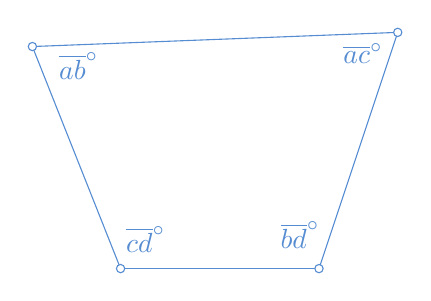
\begin{tikzpicture}[cackithi, node font= /small]
			\draw  (5.48,-1.)-- (8.,-1.);
			\draw  (8.,-1.)-- (9.,2.);
			\draw  (9.,2.)-- (4.36,1.82);
			\draw  (4.36,1.82)-- (5.48,-1.);
			\draw [fill=white] (5.48,-1.) circle (1.5pt);
			\draw (5.8,-0.63) node {$\overline{cd}^\circ$};
			\draw [fill=white] (8.,-1.) circle (1.5pt);
			\draw (7.76,-0.57) node {$\overline{bd}^\circ$};
			\draw [fill=white] (9.,2.) circle (1.5pt);
			\draw (8.56,1.73) node {$\overline{ac}^\circ$};
			\draw [fill=white] (4.36,1.82) circle (1.5pt);
			\draw (4.95,1.57) node {$\overline{ab}^\circ$};
		\end{tikzpicture}
		\vspace*{-10pt}
	\end{figure}
	\textit{Lời giải.} Do tổng bốn góc trong từ giác bằng $360^\circ,$ ta có
	\begin{align*}
		&10a + b + 10a + c + 10b + d + 10c + d \\
		= \,&20a+ 11b+11c+2d=360. \tag{$1$}
	\end{align*}
	Nhận xét rằng nếu $a\le 7$ thì  tổng trong $(1)$ không vượt quá $20\times 7 + 11\times 9 +11\times 9 + 2\times 9 =356.$ Do đó $a$ chỉ có thể nhận giá trị $8$ hoặc $9.$
	Do $b$ và $c$ có thể đổi vai trò cho nhau mà đáp án không thay đổi, ta có thể giả sử $b\ge c.$
	\vskip 0.1cm
	Trường hợp $I$: $a=8.$ Vì trong bốn góc phải có một góc không bé hơn $90^\circ$ nên $b=9.$ Phương trình $(1)$ trở thành $11c+2d=101$ và chỉ có nghiệm duy nhất là $c=9, d=1.$   
	\vskip 0.1cm
	Trường hợp $II$ $a=9$. Nếu $b\le 7$ thì tổng trong ($1$) không vượt quá $20\times 9 + 11\times 7 +11\times 7 + 2\times 9 = 352 < 360$ vô lý. Vậy $b = 8$ hoặc $b = 9$.
	\vskip 0.1cm
	Trường hợp $IIa$: $b=8.$ Phương trình $(1)$ trở thành $11c+2d=92.$ Do $c\le b=8,$ nên ta chỉ có nghiệm duy nhất $c=8, d=2.$
	\vskip 0.1cm
	Trường hợp $IIb$: $b=9.$ Phương trình $(1)$ trở thành $11c+2d=81.$ Dễ thấy phương trình chỉ có nghiệm duy nhất $c=7, d=2.$
	\vskip 0.1cm
	Tóm lại, có ba bộ bốn góc thỏa mãn bài toán: $\{\!89,\! 89,\! 91,\! 91\!\}\!,\! \{\!98,\! 98,\! 82,\! 82\!\}\!,\! \{\!99,\! 97,\! 92,\! 72\!\}.$
	\vskip 0.1cm
	{\bf\color{cackithi}OC$\pmb{32.}$} Cho hình ngũ giác đều $ABCDE$. Vẽ hai đường tròn: một có
	tâm $A$ và bán kính $AB$, và hình kia có tâm $B$ và bán kính $BA$. Gọi $X$ là giao điểm bên trong ngũ giác của hai đường tròn.
	Hỏi số đo của $\angle DEX$ bằng bao nhiêu?
	\vskip 0.1cm
	\textit{Lời giải.} Do $AX, BX, AB$ đều là bán kính của hai đường tròn nên chúng bằng nhau. Như vậy $ABX$ là tam giác đều. Vì mỗi góc trong ngũ giác đều  bằng $\frac{540^\circ}{5}=108^\circ,$ ta có $\angle EAX = 108^\circ - 60^\circ = 48^\circ.$
	\begin{figure}[H]
		\vspace*{-5pt}
		\centering
		\captionsetup{labelformat= empty, justification=centering}
		\definecolor{qqwuqq}{rgb}{0.,0.39215686274509803,0.}
		\definecolor{uuuuuu}{rgb}{0.26666666666666666,0.26666666666666666,0.26666666666666666}
		\definecolor{xdxdff}{rgb}{0.49019607843137253,0.49019607843137253,1.}
		\begin{tikzpicture}[cackithi,scale=1.2]
			\draw [shift={(1.3819660112501053,1.9021130325903073)},,color=qqwuqq,fill=qqwuqq,fill opacity=0.10000000149011612] (0,0) -- (-6.:0.6) arc (-6.:36.:0.6) -- cycle;
			\draw [] (2.,0.)-- (4.,0.);
			\draw [] (4.,0.)-- (4.618033988749895,1.9021130325903064);
			\draw [] (4.618033988749895,1.9021130325903064)-- (3.,3.077683537175253);
			\draw [] (3.,3.077683537175253)-- (1.3819660112501053,1.9021130325903073);
			\draw [] (1.3819660112501053,1.9021130325903073)-- (2.,0.);
			\draw [] (1.3819660112501053,1.9021130325903073)-- (3.,1.7320508075688772);
			\draw [] (3.,1.7320508075688772)-- (2.,0.);
			\draw [] (4.,0.)-- (3.,1.7320508075688772);
			\draw [shift={(4.,0.)},]  plot[domain=0.9272952180016115:3.4474715249946457,variable=\t]({1.*2.*cos(\t r)+0.*2.*sin(\t r)},{0.*2.*cos(\t r)+1.*2.*sin(\t r)});
			\draw [shift={(2.,0.)},]  plot[domain=-0.2992463156024767:2.2003262887940225,variable=\t]({1.*2.*cos(\t r)+0.*2.*sin(\t r)},{0.*2.*cos(\t r)+1.*2.*sin(\t r)});
			
				\draw [fill=white] (2.,0.) circle (1.5pt);
				\draw[] (1.7,-0.09) node {$A$};
				\draw [fill=white] (4.,0.) circle (1.5pt);
				\draw[] (4.3,-0.15) node {$B$};
				\draw [fill=white] (4.618033988749895,1.9021130325903064) circle (1.5pt);
				\draw[] (4.76,2.27) node {$C$};
				\draw [fill=white] (3.,3.077683537175253) circle (1.5pt);
				\draw[] (3.14,3.45) node {$D$};
				\draw [fill=white] (1.3819660112501053,1.9021130325903073) circle (1.5pt);
				\draw[] (1.2,2.29) node {$E$};
				\draw [fill=white] (3.,1.7320508075688772) circle (1.5pt);
				\draw[] (3.04,2.19) node {$X$};
		\end{tikzpicture}
		\vspace*{-10pt}
	\end{figure}
	Mặt khác, tam giác $AEX$ cân tại $A,$ nên $\angle AEX= \frac{180^\circ-48^\circ}{2}= 66^\circ.$ Ta nhận được $\angle DEX= 108^\circ - 66^\circ= 42^\circ.$
	\vskip 0.1cm
	{\bf\color{cackithi}OC$\pmb{33.}$} Seth làm $n$ viên xúc xắc giống hệt nhau bằng cách gấp $n$ bản giống như trong hình bên. Sau đó, anh ta xếp lần lượt các viên xúc xắc chồng lên nhau thành một hình tháp thẳng đứng.
	Biết rằng tổng số chấm ở mỗi một trong bốn mặt xung quanh của tháp xúc xắc đều là số lẻ. Hỏi các giá trị có thể của $n$ là bao nhiêu?
	\begin{figure}[H]
		\vspace*{-5pt}
		\centering
		\captionsetup{labelformat= empty, justification=centering}
		\hspace*{5pt}\includegraphics[height= 0.8\linewidth]{OC33}
		\includegraphics[height= 0.8\linewidth]{OC}
		\vspace*{-10pt}
	\end{figure}
	\textit{Lời giải.} Giả sử tổng số chấm trên $n$ ô của mặt đằng trước của tháp xúc xắc là $T$ và của mặt đằng sau là $S.$ Do tổng $2$ ô trên $2$ mặt đối diện của mỗi viên xúc xắc bằng $7,$ ta có $T+S=7n.$ Theo đầu bài thì cả $T$ và $S$ đều lẻ nên $n$ phải chẵn.
	\vskip 0.1cm
	Ta sẽ chứng minh rằng với mọi $n$ chẵn ta đều có thể xếp được một tháp xúc xắc như vậy. Trước tiên ta xếp $n$ viên xúc xắc theo hướng giống hệt nhau thành một tháp có mỗi mặt gồm toàn các số giống nhau. Sau đó ta xoay viên xúc xắc ở trên cùng đi sao cho các mặt trước, sau đổi chỗ cho nhau và các  mặt trái, phải cũng đổi chỗ cho nhau. 
	\vskip 0.1cm
	Bên dưới là hình minh họa trong trường hợp $n=4.$   Như vậy, tổng các chấm trên mỗi mặt của tháp có dạng $(n-1)a + 7-a=(n-2)a+7$ luôn là số lẻ. Do đó có thể xếp được tháp xúc xắc khi và chỉ khi $n$ chẵn.  
	\begin{figure}[H]
		\vspace*{-5pt}
		\centering
		\captionsetup{labelformat= empty, justification=centering}
		\includegraphics[width= 0.3\linewidth]{OC33b}
		\vspace*{-10pt}
	\end{figure}
	Trong phần cuối của chuyên mục kỳ này, chúng tôi sẽ giới thiệu với bạn đọc ba bài toán trong kỳ thi Olympic toán học trẻ  của Thổ Nhĩ Kỳ. Các bài toán này phù hợp với trình độ học sinh lớp $8-10$.
	\vskip 0.1cm
	{\bf\color{cackithi}OC$\pmb{40.}$} Cho $x, y, z$ là các số thực dương với $x\le 1.$ Chứng minh rằng
	\begin{align*}
		xy+y+2z \geq 4 \sqrt{xyz}.
	\end{align*}
	{\bf\color{cackithi}OC$\pmb{41.}$} Trong một trường có $101$ học sinh, mỗi học sinh có ít nhất một người bạn thân trong số các học sinh khác trong trường. Chứng minh rằng với mọi số nguyên $n, 1<n<101,$ ta có thể chọn một nhóm $n$ học sinh trong trường này sao cho mỗi học sinh được chọn có ít nhất một bạn thân trong số các học sinh khác được chọn. (Biết rằng nếu  $A$ là bạn thân của $B$ thì $B$ cũng là bạn thân của $A$).
	\vskip 0.1cm
	{\bf\color{cackithi} OC$\pmb{42.}$} Cho $m, n, a, k$ là các số nguyên dương và $k>1$ sao cho đẳng thức sau thỏa mãn 
	\begin{align*}
		5^m+63n+49=a^k.
	\end{align*} Tìm giá trị nhỏ nhất của $k$.
\end{multicols}

%	\newpage
%
%	\setcounter{figure}{0}
%	\thispagestyle{diendandayvahoctoannone}
\pagestyle{diendandayvahoctoan}
\everymath{\color{diendantoanhoc}}
\graphicspath{{../diendantoanhoc/pic/}}
\blfootnote{$^{1}$\color[named]{diendantoanhoc}Tòa soạn Hà Nội, Báo Thanh Niên.}
\begingroup
\AddToShipoutPicture*{\put(0,616){\includegraphics[width=19.3cm]{../bannerdiendan}}}
\AddToShipoutPicture*{\put(114,525){\includegraphics[scale=1]{../tieude.pdf}}}
\centering
\endgroup
\vspace*{188pt}

\textit{Với những ai quan tâm kỳ thi Bài giảng và bài viết về Toán học mang tên Hoàng Tụy, không chỉ là xem các thí sinh thuyết trình bài giảng, mà hơn thế, được nghe các thầy giám khảo chia sẻ quan điểm về dạy toán.}

\begin{multicols}{2}
	Theo nhận định của nhiều người theo dõi, điều lôi cuốn người xem nhất ở vòng chung khảo kỳ thi Bài giảng và bài viết về Toán học, mang tên Hoàng Tụy, là phần nhận xét của các thành viên hội đồng giám khảo. Nội dung các nhận xét này không chỉ đơn giản chỉ là những lời khen chê. Quan trọng hơn, đó là những chia sẻ về quan điểm dạy toán từ những giáo sư toán có sự am hiểu sâu sắc về toán phổ thông, thậm chí nhiều người trong đó đóng vai trò chủ chốt trong việc việc tham gia biên soạn chương trình phổ thông $2018$ như GS Đỗ Đức Thái, GS Phùng Hồ Hải. 
	\vskip 0.1cm
	\textbf{\color{diendantoanhoc}Dạy toán ứng dụng không dễ}
	\vskip 0.1cm
	Bài thuyết trình \textit{Lý thuyết đồ thị và một số cấu trúc đáng chú ý} của tác giả Hà Trung (Trường THPT chuyên Lê Hồng Phong, Nam Định) nhận được sự quan tâm đặc biệt của hội đồng giám khảo. Đây là chuyên đề (không bắt buộc) sẽ được dạy cho học sinh lớp $11$ của chương trình phổ thông $2018$ (bắt đầu được triển khai từ năm học $2023-2024$). Nhưng theo tác giả Hà Trung, lý do ông chọn chuyên đề này bởi nó có nhiều kiến thức thú vị, có nhiều ứng dụng trong cuộc sống (ví dụ bản đồ mạng lưới bay của hàng không, mạng tương tác gene). 
	\vskip 0.1cm
	Theo GS Phùng Hồ Hải thì việc tác giả ``gói" ba nội dung (sơ lược về lý thuyết đồ thị; đồ thị lưỡng phân; đồ thị cây, rừng) trong một chuyên đề là hơi ôm đồm. Hơn nữa, đối tượng mà người dạy là hướng đến học sinh giỏi toán, thì không cần thiết phải mất quá nhiều thời gian vòng vo về những ứng dụng mà nên đi thẳng sâu vào bản chất nội dung. 
	\vskip 0.1cm
	GS Ngô Việt Trung cho rằng, tác giả cần lựa chọn bài toán phù hợp với kiến thức đồ thị để giảng dạy. Không nên nhắc tới những vấn đề chỉ mang tính minh họa. Bài toán về chủ đề đồ thị thì mình phải áp dụng kiến thức đồ thị để giải quyết vấn đề. Chẳng hạn như nói về mạng thì kiến thức đồ thị đóng vai trò quan trọng. Ví dụ ChatGPT chắc chắn là phải dùng đồ thị để xác định những gì gắn với nhau. 
	\vskip 0.1cm
	Còn theo GS Đỗ Đức Thái, điều khiến cho đồ thị quan trọng hơn đối với toán học và đối với cuộc sống bây giờ là những thuật toán để từ đó giúp chúng ta tìm được câu trả lời. Chẳng hạn, người ta có thể mô tả  ở chu trình Ơ le thì có cái này, hoặc ở đồ thị lưỡng phân thì sẽ có cái thứ như thế này... Trong khi cái quan trọng phải là có thuật toán để tìm những cái đấy thế nào. Và thuật toán đó phải mô phỏng được, phải lập trình được để thành ra những cái chạy được trên máy tính. ``Có lẽ đến một lúc nào đó chúng ta nên dạy học sinh những cái như thế. Còn cứ gieo vào đầu học sinh, nhất là học sinh giỏi toán, rằng dùng cái này suy ra những cái trừu tượng này..., thì mãi cũng sẽ chẳng đi đến đâu. Cho nên tôi nghĩ nên chọn những bài toán, vẫn là toán hoàn toàn, vẫn khó như thường, nhưng cho phép người ta lập trình được, gắn vào một thuật toán nào đó coding được nó", GS Thái gợi ý. 
	\vskip 0.1cm
	\textbf{\color{diendantoanhoc}Dạy cho tử tế toán!}
	\vskip 0.1cm
	Với phần trình bày của tác giả Nguyễn Thế Minh (Trường Trung học Vinschool Imperia, Hải Phòng), chủ đề \textit{Tích hợp tư duy công dân số trong bài giảng môn Toán}, GS Đỗ Đức Thái cho rằng, bài giảng phù hợp với xu hướng tích hợp mà Chương trình phổ thông $2018$ muốn thúc đẩy. Thông qua kiến thức về toán, người dạy muốn mang đến cho người học những gợi mở ứng dụng trong lĩnh vực tin học, đó là ưu điểm của bài giảng. 
	\begin{figure}[H]
		\vspace*{-5pt}
		\centering
		\captionsetup{labelformat= empty, justification=centering}
		\includegraphics[width= 1\linewidth]{1}
		\caption{\small\textit{\color{diendantoanhoc}GS. Đỗ Đức Thái, Đại học Sư phạm Hà Nội.}}
		\vspace*{-10pt}
	\end{figure}
	Tuy nhiên, cũng từ bài giảng này, GS Thái đã cảnh báo về nguy cơ dạy học xa rời cái cốt lõi, dạy toán, mà nhiều giáo viên có thể mắc phải vì say sưa với cái gọi là ``tích hợp". Cái mà những người biên soạn Chương trình phổ thông $2018$ môn toán quan tâm là thầy cô giáo dạy toán cho học sinh, chứ không phải ra sức tô vẽ cho các bài dạy để bài học trông cho có vẻ hấp dẫn, nhưng lại không đọng lại được trong trí não người học kiến thức toán. ``Dạy toán, việc đầu tiên là dạy toán! Dạy cho tử tế toán! Rồi muốn làm việc gì thì làm sau. Học sinh học môn toán thì trước hết các em phải được học toán", GS Thái khẳng định. 
	\vskip 0.1cm
	\textbf{\color{diendantoanhoc}Phải tuân thủ những chuẩn mực} 
	\vskip 0.1cm
	Với phần trình bày của tác giả Nguyễn Thụy Việt Anh (Trường Liên cấp Hội nhập Quốc tế Ischool, Quảng Trị), về \textit{Hình có trục đối xứng}, GS Đỗ Đức Thái cảnh báo, người giáo viên luôn cần xác định một bài học cụ thể thuộc dạng nào trong lý thuyết dạy học. Trong trường sư phạm, giáo sinh được dạy cách xác định dạng bài điển hình trong lý thuyết dạy học. Bởi mỗi dạng bài điển hình sẽ có một nguyên tắc dạy học mà người dạy phải bám theo nguyên tắc đó, giống như đi đường thì phải đi bên phải.  
	\vskip 0.1cm
	``Dạy toán có những chuẩn mực về mặt sự phạm. Đây là bài học về dạy khái niệm mới, định nghĩa mới. Ở bài này, GV dạy một khái niệm rất khó với học sinh, đó là hình có trục đối xứng, hay nói cách khác, đối xứng trục mà lại không được phép định nghĩa phép đối xứng trục (vì lên đến lớp $10$ học sinh mới được học kiến thức này ở chuyên đề). Nguyên tắc dạy bài học khái niệm mới, định nghĩa mới, bao gồm nhiều bước, trong đó bước cuối cùng là làm nổi bật lên được là chốt lại, neo lại trong đầu học sinh khái niệm mới đó là cái gì", GS Thái phát biểu. 
	\vskip 0.1cm
	\textbf{\color{diendantoanhoc}Học toán để làm gì?} 
	\vskip 0.1cm
	Ngay từ bài giảng đạt giải cao nhất (giải nhì, không có giải nhất) trong phần \textit{Tìm hiểu về môn Toán trong ``Chương trình giáo dục phổ thông mới" thông qua một chủ đề cụ thể}, các thí sinh và người theo dõi cuộc thi cũng được nhận những chia sẻ thấu đáo về quan điểm dạy toán của những người tham gia biên soạn chương trình môn toán. Đây là bài giảng \textit{Giải bài toán tập hợp bằng phương pháp ``ô ăn quan"}, của nhóm tác giả Ngô Quốc Trung, Nguyễn Thị Hiền (Trường Liên cấp Hermann Gmeiner Vinh, Nghệ An). Phần đầu bài giảng, các tác giả dùng phương pháp ô ăn quan để giải các bài toán ở tiểu học (thường được gọi là bài toán giả thiết tạm). ``Tôi thấy phần đó rất thú vị, rất sáng tạo. Nó cho học sinh thấy một cơ chế mà thoát ra khỏi bản chất giải phương trình. Tôi hoàn toàn cho điểm $10$ ở phần đó", GS Thái nhận xét.
	\vskip 0.1cm
	Nhưng với phần thứ hai, các tác giả dùng phương pháp này với nội dung tổ hợp ở lớp $10$, thì các tác giả không thuyết phục được ban giám khảo. ``Nói cho cùng, học toán là học cách nghĩ, cách suy luận, cách khám phá ra một cái gì đó. Từ nó dẫn người ta đến tư duy, đến những thuật toán chung, để khái quát nó lên, giải quyết những mô hình trong cuộc sống mà nó tương tự như thế. Việc dùng một phương pháp thiên về mô tả cho nội dung tổ hợp ở lớp 10 của các tác giả vừa khiến cho bài giảng cầu kỳ, vừa không phù hợp.  Học sinh lớp $10$, $15-16$ tuổi rồi, không phải lúc nào cũng cầm nắm sờ mó với mô tả được. Một lúc nào đó, anh phải chuyển từ \textit{cụ thể} lên đến \textit{hình ảnh}, rồi lên đến \textit{biểu tượng hoá} chứ.",  GS Thái chia sẻ.
	\vskip 0.1cm
	\PIbox{Cuối tháng Ba vừa qua, trong trong khuôn khổ sự kiện "Toán học cho mọi người",  vòng chung khảo kỳ thi Bài giảng và bài viết về Toán học, mang tên Hoàng Tụy, lần thứ hai, đã được diễn ra. Trước đó, hội đồng giám khảo đã tiến hành chấm các hồ sơ dự thi ở vòng sơ khảo, lựa chọn được $8$ hồ sơ tốt nhất để tranh tài tại vòng chung khảo. Tại vòng chung khảo (diễn ra ở hội trường Hoàng Tụy, Viện Toán học Việt Nam),  đại diện nhóm tác giả hoặc các tác giả đã \linebreak thuyết trình các bài giảng và bài viết trước}
	
	\PIbox{hội đồng giám khảo, trước sự theo dõi (trực tiếp và trực tuyến) của những người quan tâm tới kỳ thi. Theo hội đồng giám khảo, chất lượng hồ sơ dự thi năm nay cao hơn hẳn năm trước, vì thế mà phần trình bày của $8$ thí sinh được lựa chọn thuyết trình trong vòng chung khảo ít nhiều đều tạo sự thú vị cho người theo dõi. 
	\vskip 0.1cm	
	Trọng tâm nội dung của kỳ thi lần thứ hai là Tìm hiểu về môn Toán trong ``Chương trình giáo dục phổ thông mới" thông qua một chủ đề cụ thể. Bên cạnh đó là một số nội dung truyền thống như: Tìm hiểu về Toán sơ cấp, lịch sử Toán học và Toán học trong cuộc sống. 
	\vskip 0.1cm	
	Hội đồng giám khảo năm nay gồm GS Ngô Việt Trung, Chủ tịch Hội Toán học Việt Nam, nguyên Viện trưởng Viện Toán học; GS Đỗ Đức Thái, Trường ĐH Sư phạm Hà Nội; GS Phùng Hồ Hải, Phó chủ tịch Hội Toán học Việt Nam, nguyên Viện trưởng Viện Toán học; GS Hà Huy Khoái, nguyên Viện trưởng Viện Toán học; TS Trần Nam Dũng, Phó hiệu trưởng Trường Phổ thông Năng khiếu, ĐH Quốc gia TP.HCM; PGS Phó Đức Tài, Trưởng Khoa Toán-Cơ-Tin học, Trường ĐH Khoa học Tự nhiên, ĐH Quốc gia Hà Nội. }
	\vskip 0.1cm
	\textbf{\color{diendantoanhoc}Kết quả chung cuộc như sau:}
	\vskip 0.1cm
	\textit{Nội dung ``Tìm hiểu về môn Toán trong ``Chương trình giáo dục phổ thông mới" thông qua một chủ đề cụ thể": }
	\vskip 0.1cm
	$\bullet$	Giải nhì (không có giải nhất): Bài giảng ``Giải bài toán tập hợp bằng phương pháp ``ô ăn quan" của nhóm tác giả Ngô Quốc Trung, Nguyễn Thị Hiền, Trường Liên cấp Hermann Gmeiner Vinh, Nghệ An. 
	\vskip 0.1cm
	$\bullet$	Giải ba: Bài viết ``Một cách thiết kế dạy học Toán theo hướng gắn liền với thực tiễn", tác giả Phạm Đức Quang, Trường ĐH Sư phạm Hà Nội $2$.
	\vskip 0.1cm 
	$\bullet$	Giải khuyến khích: Bài giảng ``Hình có trục đối xứng", tác giả Nguyễn Thụy Việt Anh, Trường Liên cấp Hội nhập Quốc tế Ischool, Quảng Trị; Bài giảng ``Tích hợp tư duy công dân số trong bài giảng môn Toán", tác giả Nguyễn Thế Minh, Trường Trung học Vinschool Imperia, Hải Phòng.
	\vskip 0.1cm
	\textit{Các nội dung khác:}
	\vskip 0.1cm 
	$\bullet$	Giải nhất: Bài giảng ``Bổ đề hai đoạn thẳng và một số ứng dụng", tác giả Nguyễn Hữu Tâm, Trường THPT chuyên Lê Quý Đôn, Bình Định. 
	\vskip 0.1cm
	$\bullet$	Giải nhì: Bài giảng ``Mập mờ công thức Euler", tác giả Nguyễn Quang Minh, Biên Hoà, Đồng Nai. 
	\vskip 0.1cm
	$\bullet$	Giải ba: Bài giảng ``Lý thuyết đồ thị và một số cấu trúc đáng chú ý", tác giả Hà Trung, Trường THPT chuyên Lê Hồng Phong, Nam Định. 
	\vskip 0.1cm
	$\bullet$	Giải khuyến khích: Bài giảng ``Nét đẹp của phương pháp đếm dưới góc nhìn của số Fibonacci", tác giả Nguyễn Tuấn Anh, Trường PTTH chuyên Nguyễn Quang Diêu, Đồng Tháp. 
\end{multicols}
%	\newpage
%	
%	\thispagestyle{empty}
%	\begingroup 
%	\AddToShipoutPicture*{\put(0,0){\includegraphics[width=19.3cm]{MV.pdf}}}
%	\centering
%	\vspace*{0cm}
%	\endgroup
%	\newpage	
%	\pagestyle{empty}
%	
%	\setcounter{figure}{0}
%	\thispagestyle{lichsutoanhocnone}
\pagestyle{lichsutoanhoc}
\graphicspath{{../lichsutoanhoc/pic/}}
\everymath{\color{lichsutoanhoc}}
\blfootnote{$^1$\color{lichsutoanhoc}Cộng tác viên Viện Toán học.}
\begingroup
\AddToShipoutPicture*{\put(0,616){\includegraphics[width=19.3cm]{../bannerlichsu}}}
\AddToShipoutPicture*{\put(104,525){\includegraphics[scale=1]{../tieude.pdf}}}
\centering
\endgroup

\vspace*{185pt}

\begin{multicols}{2}
	\textbf{\color{lichsutoanhoc}Nhập đề.}
	Chúng ta có rất ít thông tin về cuộc đời các nhà toán học Hy Lạp vĩ đại. Euclid cũng không ngoại lệ. Tất cả những gì được biết về ông chứa trong một vài câu tóm tắt của Proclus: (Euclid, người đã viết \textit{Cơ sở} (\textit{Elements}), trong đó tập hợp nhiều định lý của Eudoxus, hoàn thiện nhiều kết quả của Theaetetus, đồng thời đã chứng minh rõ ràng, chặt chẽ và sắp xếp lại trong một trật tự logic rất nhiều kết quả chỉ được chứng minh một cách lỏng lẻo bởi những người đi trước.)
		\begin{figure}[H]
		\vspace*{-5pt}
		\centering
		\captionsetup{labelformat= empty, justification=centering}
		\includegraphics[width= 1\linewidth]{1}
		\vspace*{-10pt}
	\end{figure}
	Như vậy, ngay cả nhà triết học Proclus ($411-485$ Công nguyên, viết tắt: CN), người đã viết nhiều cuốn sách về triết học và toán học Hy Lạp, trong đó có cuốn sách bình luận về \textit{Cơ sở} của Euclid [$8$], cũng không cho biết chính xác năm sinh, năm mất và nơi sinh của Euclid. Proclus chỉ cho biết Euclid trẻ hơn các học trò đầu tiên của Plato, nhiều tuổi hơn Eratosthenes và Archimedes. Plato mất vào năm $347$ trước Công nguyên (viết tắt: TCN) và Archimedes sống trong khoảng năm $287$ đến $212$ TCN. Vì vậy, các nhà viết sử cho rằng Euclid sống vào khoảng những năm $300$ TCN, dưới thời Ptolemy I, người trị vì từ $306$ đến $283$ TCN và Ptolemy II ($309-246$ TCN, người trị vì từ $284$ đến $246$ TCN). 
	\vskip 0.1cm
	Phần đầu bài viết này giới thiệu nội dung cơ bản và những đánh giá về \textit{Cơ sở} và các tác phẩm khác của Euclid, chủ yếu dựa trên [$1$]. Các phần sau dựa trên sự tổng hợp của các tài liệu [$1$]--[$8$].
	\vskip 0.1cm
	\textbf{\color{lichsutoanhoc}Bối cảnh ra đời của Elements.}
	Alexander Đại đế đã chinh phục phần lớn thế giới trong vòng $12$ năm ($334-323$ TCN). Vì quân đội của ông chủ yếu là người Hy Lạp nên ông đã truyền bá văn hóa Hy Lạp sang một phần rộng lớn của vùng Cận Đông. Tiếp theo là một chương mới của lịch sử, được gọi là \textit{Thời đại Hy Lạp hóa} (Hellenistic) hoặc \textit{tựa Hy Lạp} (Greek--like), kéo dài trong ba thế kỷ, cho đến khi đế chế La Mã được thành lập.
	\vskip 0.1cm
	Sau khi Alexander qua đời, Ptolemy, một trong những vị tướng hàng đầu của Alexander, trở thành Thống đốc của Ai Cập và hoàn thành việc xây dựng thành phố Alexandria. Alexandria nhanh chóng tỏa sáng và làm lu mờ Athens, khiến Athens bị giảm xuống vị thế của một thành phố tỉnh lẻ. Trong gần $1000$ năm, Alexandria là trung tâm phát triển của văn hóa Hy Lạp hóa.
	\vskip 0.1cm
	Các thế hệ vua Ptolemy đã làm hết mình để biến Alexandria thành trung tâm của đời sống trí thức cho toàn bộ Địa Trung Hải. Họ đã xây dựng một trung tâm lớn của học thuật, gọi là \textit{Bảo tàng} (Musaeum), ở đây có nghĩa là \textit{Ngôi đền của các nàng thơ} (Temple of the Muses), tiền thân của trường đại học hiện đại. Các học giả hàng đầu của thời đại--các nhà khoa học, nhà thơ, nghệ sĩ và nhà văn--đã đến Alexandria theo lời mời của các vua Ptolemy với lòng hiếu khách đặc biệt. Các học giả có thể ở lại \textit{Bảo tàng} bao lâu tùy thích, Tại \textit{Bảo tàng}, họ có thời gian rảnh rỗi để theo đuổi việc nghiên cứu, tiếp cận các sách cổ trong thư viện và có cơ hội thảo luận các vấn đề với các chuyên gia.  Ngoài ăn ở miễn phí, họ được trả lương, với yêu cầu duy nhất là họ phải giảng bài. Các học giả sống trong \textit{Bảo tàng} với chi phí của nhà vua trong điều kiện sang trọng, với các phòng giảng rộng rãi và lộng lẫy, có thể đi dạo trong các hành lang với các hàng cột tráng lệ. Bảo tàng có một phòng ăn rộng lớn, nơi các học giả dùng bữa cùng nhau. 
	\vskip 0.1cm
	Được xây dựng như một tượng đài cho sự huy hoàng của dòng họ Ptolemy, \textit{Bảo tàng} đã là một cột mốc quan trọng trong lịch sử khoa học. Nó được xây dựng như là một tổ chức nghiên cứu và học thuật, hơn là một cơ quan giáo dục, cho các học giả và các nhà khoa học đến sống và làm việc tại đây hàng mấy thế kỷ. Ở đỉnh cao của nó, trung tâm này có đến vài trăm chuyên gia, sự hiện diện của họ đã thu hút nhiều thế hệ trẻ háo hức đến học tập và phát triển tài năng. Khoa học và toán học thời kỳ này đã phát triển với thành công đáng kể. Trong lịch sử toán học chỉ có một thời gian khác trong khoảng $200$ năm có thể so sánh với giai đoạn $300-100$ trước Công nguyên, đó là khoảng thời gian từ Kepler đến Gauss ($1600-1850$).
	\begin{figure}[H]
		\vspace*{-10pt}
		\centering
		\captionsetup{labelformat= empty, justification=centering}
		\includegraphics[width= 1\linewidth]{2}
		\caption{\small\textit{\color{lichsutoanhoc}Một trang từ cuốn sách Elements của Euclid in lần đầu tiên bằng tiếng Latin năm $1482$.}}
		\vspace*{-10pt}
	\end{figure} 
	Các học giả không thể sống mà không có sách, vì vậy nhu cầu đầu tiên là thu thập các bản thảo. Được thành lập gần như đồng thời với \textit{Bảo tàng} và liền kề với nó là \textit{Thư viện lớn} của Alexandria, nơi chứa bộ sưu tập lớn nhất các tác phẩm Hy Lạp còn tồn tại. Tất nhiên trước đó đã có những thư viện, nhưng không có thư viện nào sở hữu những tài nguyên lớn như thư viện Alexandria. Các bản thảo được tìm kiếm trên khắp thế giới và có những đại lý được ủy quyền để sao chép các tác phẩm nếu không mua được chúng. Du khách đến Alexandria được yêu cầu giao nộp bất kỳ cuốn sách nào chưa có trong thư viện.
	\vskip 0.1cm
	Trước khi Bảo tàng chìm vào quên lãng năm $641$, nó đã tạo ra nhiều tác phẩm nổi bật của các học giả, xác định tiến trình phát triển của toán học trong nhiều thế kỷ: Euclid, Archimedes, Apollonius, Ptolemy và Diophantus.
	\vskip 0.1cm
	Các nhà lịch sử thống nhất cho rằng, Euclid là một học giả tích cực của \textit{Bảo tàng} và \textit{Thư viện}, dưới triều đại Ptolemy I và II. 
	\vskip 0.1cm
	Hậu thế biết đến Euclid như là tác giả của \textit{Cơ sở của hình học} (\textit{Elements of Geometry}), một cuốn sách toán học quan trọng nhất của văn hóa Hy Lạp và có lẽ của tất cả các thời đại. \textit{Cơ sở} là tập hợp các kiến thức quan trọng nhất vào thời điểm đó, được sắp xếp thành $13$ phần, hay $13$ chương ($13$ quyển). Sáu quyển đầu dành cho hình học phẳng, ba quyển tiếp theo về số học. Quyển X cung cấp mối liên hệ giữa hai đại lượng: độ lớn (magnitude) được trình bày trong Quyển V và các con số (number) trong quyển VII. Quyển XI nghiên cứu hình học không gian và Quyển XII trình bày phương pháp vét cạn (method of exhaustion) cho cả hình phẳng và hình không gian. Và cuối cùng, Quyển XIII trình bày năm khối đa diện đều và phân loại các đường đã được trình bày trong Quyển X.   
	\vskip 0.1cm
	Mặc dù đã có một vài cuốn sách toán trước \textit{Cơ sở}, nhưng không quyển nào được bảo  tồn, vì lý do rõ ràng là tất cả đã bị lu mờ và được thay thế bởi cuốn sách của Euclid.
	\vskip 0.1cm
	Mặc dù phần lớn kết quả đã có từ trước, nhưng sự sắp xếp hợp lý đến tuyệt vời của các định lý và sự phát triển của các sự kiện cho thấy thiên tài của Euclid. Ông đã hợp nhất các khám phá biệt lập thành một hệ thống các định đề, định nghĩa và tiên đề ban đầu, để từ đó suy ra các kết quả (định lý) theo một thứ tự suy diễn duy nhất.
	\vskip 0.1cm
	Gần như không có cuốn sách nào quan trọng đối với tư tưởng và giáo dục của phương Tây hơn là \textit{Cơ sở} của Euclid. Hiếm có cuốn sách nào, ngoại trừ Kinh Thánh, đã được xuất bản, lưu hành và nghiên cứu rộng rãi như \textit{Cơ sở}. Trong suốt $2000$ năm, sáu cuốn sách đầu tiên của \textit{Cơ sở} là  sách giáo khoa hình học của học sinh. Hơn $1000$ phiên bản của \textit{Cơ sở} đã xuất hiện kể từ bản in đầu tiên bằng tiếng Latin ra đời năm $1482$. Và trước đó, các bản sao viết tay đã thống trị phần lớn việc giảng dạy toán học ở châu Âu.
	\begin{figure}[H]
		\vspace*{-5pt}
		\centering
		\captionsetup{labelformat= empty, justification=centering}
		\includegraphics[width= 1\linewidth]{3}
		\caption{\small\textit{\color{lichsutoanhoc}Bìa trước của bản dịch tiếng Anh đầu tiên của Henry Billingsley năm $1570$.}}
		\vspace*{-10pt}
	\end{figure} 
	Mặc dù danh tiếng của Euclid, cả trong thời cổ đại và thời hiện đại, hầu như chỉ dựa vào \textit{Cơ sở}, nhưng ông còn là tác giả của ít nhất $10$ tác phẩm khác về nhiều chủ đề khác nhau. Văn bản tiếng Hy lạp cuốn \textit{Dữ liệu} (\textit{Data}), một tuyển tập gồm $95$ bài tập có lẽ dành cho những sinh viên đã hoàn thành \textit{Cơ sở}, là văn bản duy nhất khác của Euclid về hình học còn tồn tại. Một chuyên luận, \textit{Các thiết diện conic} (\textit{Conic Sections}), là nền tảng của bốn cuốn sách đầu tiên trong tác phẩm cùng tên của Apollonius, đã bị thất lạc. Và tác phẩm \textit{Các hệ quả} (\textit{Porisms}) cũng  chung số phận. Rõ ràng \textit{Các thiết diện conic} là một cuốn sách về hình học cao cấp, là một bản cổ xưa nhất của hình học giải tích. Ngoài ra, ông còn có \textit{Phân chia các  hình} (\textit{Division of Figures}), \textit{Hiện tượng} (\textit{Phaenomena}), và \textit{Quang học} (\textit{Optics}),...
	\vskip 0.1cm
	Chúng ta biết rất ít về cuộc sống cá nhân của Euclid.  Chỉ biết chắc chắn ông đã thành lập một trường học và giảng dạy ở Alexandria, nhưng không có gì khác được biết ngoại trừ điều đó. Có khả năng ông đã được đào tạo toán học ở Athens dưới sự dẫn dắt của các học trò của Plato. Hai giai thoại sau có thể là những minh chứng cho tính cách của Euclid. Giai thoại thứ nhất kể rằng, khi nhà vua Ptolemy I hỏi ông liệu có con đường nào ngắn để tiếp thu hình học hơn là \textit{Cơ sở} không, ông đã trả lời: ``Thưa Bệ hạ, không có con đường hoàng gia tới hình học" (``There is no royal road to Geometry"), ngụ ý là toán học bình đẳng với tất cả mọi người, Một câu chuyện khác, do Stobaeus (thế kỷ $5$) kể lại, liên quan đến một thanh niên bắt đầu học hình học với Euclid và hỏi, sau khi đã học các định lý đầu tiên: ``Nhưng tôi sẽ nhận được gì sau khi học những điều này?" Euclid đã gọi người hầu của mình đến và bảo rằng: ``Hãy cho người đàn ông này một đồng xu, vì anh ta phải kiếm được lợi nhuận từ những gì anh ta học được." Lời quở trách có lẽ đã được chuyển thể từ một câu châm ngôn của trường phái Pythagoras: ``Một sơ đồ và một bước (trong kiến thức), không phải là một sơ đồ và một đồng xu." (``A diagram and a step (in knowledge), not a diagram and a coin.")  
	Thiết nghĩ những câu chuyện này vẫn còn mang tính thời sự đến tận ngày nay.
	\vskip 0.1cm
	\textbf{\color{lichsutoanhoc}Cơ sở hình học của Euclid}
	\vskip 0.1cm
	Trong hơn hai nghìn năm, Euclid đã là người phát ngôn của hình học Hy Lạp, sự sáng tạo tuyệt vời nhất của trí tuệ Hy Lạp. Kể từ thời của ông, việc nghiên cứu \textit{Cơ sở} là điều cần thiết với một nền giáo dục khai phóng. Thế hệ này qua thế hệ khác đã coi \textit{Cơ sở} là đỉnh cao của logic, và nghiên cứu nó là cách tốt nhất làm cơ sở cho suy luận chính xác.  Chỉ trong vòng $100$ năm trở lại đây, \textit{Cơ sở} mới bắt đầu bị thay thế bởi các sách giáo khoa hiện đại. Tuy nhiên, tác phẩm của Euclid vẫn là mô hình tối cao về toán học thuần túy.
	\vskip 0.1cm
	Bất kỳ ai quen thuộc với quá trình thao tác trí tuệ đều nhận ra rằng nội dung của \textit{Cơ sở} không thể là nỗ lực của một cá nhân đơn lẻ. Có lẽ không nhiều các định lý được thiết lập trong \textit{Cơ sở} là do chính Euclid khám phá ra. Sự vĩ đại của Euclid nằm ở chỗ ông đã sắp xếp một khối lượng lớn các kiến thức độc lập của toán học Hy Lạp về hình học và lý thuyết số vào một trật tự logic chặt chẽ, có quan hệ mật thiết với nhau. Kết quả này tiếp nối kết quả khác với tối thiểu các giả thiết. Uy tín của \textit{Cơ sở} lớn đến mức tác giả của nó hiếm khi được gọi bằng tên mà bằng \textit{Tác giả của Elements} hoặc đơn giản là \textit{Nhà hình học}.
	\vskip 0.1cm 
	Euclid nhận thức được rằng để tránh vòng luẩn quẩn và cung cấp một điểm khởi đầu, một số sự kiện về bản chất của đối tượng phải được coi là một sự thật hiển nhiên mà không cần chứng minh, được gọi là các \textit{tiên đề}. Theo một nghĩa nào đó, chúng là những ``luật chơi" mà từ đó tất cả các suy luận có thể tiến hành, là nền tảng mà toàn bộ các định lý phải dựa vào.
	\vskip 0.1cm
	Euclid đã cố gắng xây dựng toàn bộ tòa nhà kiến thức hình học Hy Lạp, được tích lũy kể từ thời Thales, trên $5$ định đề có bản chất hình học cụ thể và $5$ tiên đề được dùng làm nền móng cho toàn bộ lâu đài toán học. Ba định đề đầu tiên là định đề xây dựng, khẳng định những gì chúng ta được phép vẽ. Từ đó, ông suy ra từ $10$ giả định này $465$ mệnh đề qua một chuỗi suy luận logic, sử dụng chúng như những viên đá lót đường trong một cuộc diễu hành có trật tự từ một mệnh đề đã được chứng minh sang một mệnh đề khác. Điều kỳ diệu là rất nhiều mệnh đề thú vị có thể thu được chỉ từ một vài tiên đề được lựa chọn một cách  khôn ngoan. 
	\vskip 0.1cm
	Đột ngột và không có bình luận giới thiệu, cuốn sách đầu tiên của \textit{Cơ sở} mở ra với danh sách $23$ định nghĩa (xem [$2b$], trang $16-18$). Chúng bao gồm, thí dụ, điểm là gì, đường là gì (Định nghĩa $1$, $2$) và kết thúc bằng Định nghĩa $23$: ``Các đường thẳng song song là các đường thẳng cùng nằm trong một mặt phẳng và khi kéo dài đến vô tận ở cả hai hướng thì không gặp nhau ở cả hai hướng." Các định nghĩa này không được coi là định nghĩa theo nghĩa hiện đại. Mặc dù mơ hồ và không hữu ích trong một số khía cạnh, chúng cũng đủ để tạo ra một số hình ảnh trực quan nhất định. Một số thuật ngữ kỹ thuật được sử dụng, thí dụ chu vi đường tròn, hoàn toàn không được định nghĩa. Thật lạ lùng khi Euclid đã định nghĩa đường thẳng song song, lại không đưa ra một định nghĩa chính thức về hình bình hành.
	\vskip 0.1cm
	Sau các định nghĩa, Euclid đặt ra $10$ nguyên tắc mà chứng minh các mệnh đề và định lý phải dựa trên. Đó là (xem thêm [$2b$], trang $19-20$):
	\vskip 0.1cm
	\textbf{\color{lichsutoanhoc}Các định đề:}
	\vskip 0.1cm
	$1.$ Cùng quy ước rằng có thể vẽ một đoạn thẳng nối hai điểm bất kỳ.
	\vskip 0.1cm
	$2.$ Và có thể kéo dài liên tục một đoạn thẳng thành đường thẳng.
	\vskip 0.1cm
	$3.$ Có thể vẽ một đường tròn có tâm và bán kính bất kỳ.
	\vskip 0.1cm
	$4.$ Tất cả các góc vuông đều bằng nhau.
	\vskip 0.1cm
	$5.$ Nếu một đường thẳng cắt hai đường thẳng khác tạo thành các góc trong về cùng một phía [với nó] có tổng nhỏ hơn $2$ góc vuông, thì hai đường thẳng (bị cắt) khi kéo dài ra vô tận sẽ cắt nhau ở phía của đường thẳng ban đầu mà tổng các góc trong nhỏ hơn $2$ vuông (chứ không cắt ở phía bên kia). 
	\vskip 0.1cm
	\textbf{\color{lichsutoanhoc}Các tiên đề:}
	\vskip 0.1cm
	$1.$ Những thứ cùng bằng một thứ thì bằng nhau.
	\vskip 0.1cm
	$2.$ Nếu cùng thêm những thứ bằng nhau vào những thứ bằng nhau thì những tổng sẽ bằng nhau.
	\vskip 0.1cm
	$3.$ Nếu cùng bớt những thứ bằng nhau vào những thứ bằng nhau thì những phần còn lại sẽ bằng nhau.
	\vskip 0.1cm
	$4.$ Các thứ trùng nhau thì bằng nhau.
	\vskip 0.1cm
	$5.$ Tổng thể thì lớn hơn bộ phận.
	\vskip 0.1cm
	Định đề $5$, còn gọi là \textit{Định đề song song}, đã trở thành một trong những phát biểu nổi tiếng và gây tranh cãi nhất trong lịch sử toán học. Thậm chí có ý kiến cho rằng Euclid không hoàn toàn hài lòng với Định đề $5$. Ông đã trì hoãn sử dụng của nó cho đến khi không thế tiến xa hơn nếu không có nó, mặc dù việc sử dụng nó sớm hơn sẽ đơn giản hóa nhiều chứng minh các định lý.
	\vskip 0.1cm
	Hơn $2000$ năm, từ lúc xuất hiện \textit{Cơ sở} đến thế kỷ $19$, các nhà toán học đã cố gắng rút ra định đề song song từ bốn định đề đầu tiên, tin rằng bốn định đề này cùng với $5$ tiên đề là đủ cho sự phát triển hoàn chỉnh hình học Euclid. Tất cả những nỗ lực nhằm thay đổi trạng thái từ ``Định đề $5$" thành định lý" đều thất bại, vì mỗi nỗ lực đều dựa trên giả định ẩn tương đương với chính định đề đó. 
	\vskip 0.1cm
	Tuy nhiên, những nỗ lực này đã dẫn đến việc phát hiện ra hình học phi--Euclid, trong đó các Định đề của Euclid, ngoại trừ định đề song song đều đúng và các định lý của Euclid đều đúng, ngoại trừ những định lý dựa trên định đề song song. Thiên tài của Euclid thể hiện ở chỗ ông đã nhận ra rằng Định đề $5$ đòi hỏi tuyên bố rõ ràng như một giả định, không thể được chứng minh.   
	\vskip 0.1cm
	Khi xem xét Định đề $5$ Euclid, nhà toán học Giovanni Saccheri $(1667-1733)$ đã phân loại:
	\vskip 0.1cm
	Trường hợp $1$: Qua điểm đã cho có duy nhất đường thẳng song song với đường thẳng đã cho.
	\vskip 0.1cm
	Trường hợp $2$: Qua điểm đã cho có nhiều hơn một đường thẳng song song với đường thẳng đã cho.
	\vskip 0.1cm
	Trường hợp $3$: Qua điểm đã cho không có đường thẳng nào song song với đường thẳng đã cho.
	\vskip 0.1cm
	Trường hợp $1$ cho ta hình học Euclid, Trường hợp $2$ dẫn đến hình học Lobachevsky, Trường hợp $3$ cho ta hình học Riemann.
	\vskip 0.1cm
	Việc xem xét kỹ lưỡng trong hơn $2000$ năm đã phát lộ nhiều điểm sáng và những nhược điểm trong cách xử lý hình học của Euclid. Hầu hết các định nghĩa của ông đều dễ bị chỉ trích trên cơ sở này hay cơ sở khác. Xét cho cùng, một định nghĩa chỉ mang lại ý nghĩa của một từ theo nghĩa khác, đơn giản hơn--hoặc những từ mà ý nghĩa của nó đã rõ ràng. Những từ này đến lượt chúng lại được định nghĩa bằng những từ thậm chí còn đơn giản hơn. Rõ ràng quá trình định nghĩa như vậy phải có kết thúc. Cách duy nhất để tránh một vòng tròn luẩn quẩn là cho phép một số khái niệm ban đầu không được định nghĩa.
	Euclid đã nhầm khi cố gắng giải nghĩa toàn bộ từ vựng mà ông đã sử dụng. Chắc chắn điều này dẫn tới một số định nghĩa kỳ lạ và không thỏa đáng. Thí dụ: ``Điểm là cái không thể chia nhỏ", ``Đường không có chiều rộng". Vậy ``chia nhỏ" và ``chiều rộng" là gì? Ý tưởng về ``điểm" và ``đường thẳng" là những khái niệm cơ bản nhất trong hình học, chúng có thể được mô tả và được giải thích nhưng không thể được định nghĩa thỏa đáng bằng các định nghĩa đơn giản hơn chính chúng. Phải có một sự khởi đầu ở đâu đó trong một hệ thống khép kín, vì vậy chúng nên được chấp nhận không có định nghĩa.
	\vskip 0.1cm
	Có lẽ sự phản đối lớn nhất đã được đưa ra chống lại tác giả \textit{Cơ sở} là sự bất cập đáng tiếc trong các tiên đề của ông. Ngoài những thiếu sót hiển nhiên như  không nêu được sự tồn tại của điểm và đường thẳng hoặc đường thẳng nối hai điểm là duy nhất, Euclid đã đưa ra một số giả định ngầm được sử dụng sau này trong các chứng minh nhưng không xuất phát từ các định đề. Khá nhiều chứng minh của Euclid dựa trên hình vẽ và bằng chứng trực quan. Điều này được minh họa bằng lập luận được sử dụng ngay trong mệnh đề đầu tiên dưới đây trong \textit{Cơ sở}.
	\vskip 0.1cm 
	\textbf{\color{lichsutoanhoc}Mệnh đề} $\pmb{1}$ Cho một đoạn $AB$. Tồn tại tam giác đều có đoạn thẳng là một trong các cạnh của nó.
	\vskip 0.1cm
	\textbf{\color{lichsutoanhoc}Chứng minh} Sử dụng Định đề $3$, vẽ đường tròn tâm $A$ bán kính $AB$ đi qua điểm $B$. Từ tâm $B$ vẽ đường tròn bán kính $BA$ đi qua $A$. Từ giao điểm $C$ của hai đường tròn, dựng đoạn thẳng $CA$ và $CB$ (Định đề $1$).  Ta thấy $AC=AB$ và $BC=AB$ vì chúng là các bán kính của một đường tròn. Từ Tiên đề $1$ suy ra $AC=AB=BC$. Vậy các đoạn thẳng $AB, AC, BC$ tạo thành tam giác đều có đoạn thẳng $AB$ cho trước là một cạnh.
	\vskip 0.1cm
	\textbf{\color{lichsutoanhoc}Lời bình.} Ở đây có một vấn đề: Trên cơ sở trực giác, ta thấy hai đường tròn tâm $A$ và tâm $B$ chắc chắn cắt nhau tại $C$.  Tuy nhiên, mục đích của một lý thuyết tiên đề chính xác là phải cung cấp một hệ thống lý luận không phụ thuộc vào trực giác. Toàn bộ chứng minh sẽ đổ bể nếu các đường tròn ta xây dựng là không cắt nhau. Và điều này (đường tròn cắt nhau) không thể suy ra từ các định đề và tiên đề. Để khắc phục tình trạng này, phải bổ sung thêm một định đề đảm bảo tính ``liên tục" của các đường thẳng và đường tròn. Các nhà toán học sau này đã phải bổ sung thêm:
	\vskip 0.1cm
	\textit{Nếu một đường tròn hoặc đường thẳng có một điểm ở ngoài và một điểm ở trong một đường tròn khác thì nó có hai điểm chung với đường tròn.}
	\vskip 0.1cm 
	Phát biểu đơn thuần của định đề liên quan đến các khái niệm ``bên trong" và ``bên ngoài" không xuất hiện rõ ràng trong \textit{Cơ sở}. Nếu hình học muốn phát huy hết danh tiếng của nó về tính chặt chẽ logic hoàn hảo, thì nó phải chú ý đáng kể đến ý nghĩa của các thuật ngữ đó và các tiên đề chi phối chúng. 
	\vskip 0.1cm
	Trong suốt $25$ năm cuối của thế kỷ $19$, nhiều nhà toán học đã cố gắng xây dựng một hệ tiên đề đầy đủ và cần thiết để chứng minh tất cả các định lý quen thuộc từ lâu trong hình học Euclid. Nghĩa là, họ đã cố gắng bổ sung thêm những định đề nhằm mang lại tính rõ ràng và chặt chẽ cho những ý tưởng mà Euclid đã nhận ra bằng trực giác.  Người thành công nhất trong lĩnh vực này là David Hilbert ($1862-2943$) với tác phẩm \textit{Cơ sở Hình học} in năm $1899$ [$9$] (Grundlagen der Geometrie, tiếng Anh: \textit{Foundations of Geometry}). Trong tác phẩm này, Hilbert đã xây dựng lại hình học Euclid dựa trên năm nhóm tiên đề: các tiên đề về tính liên thông, các tiên đề về thứ tự, Tiên đề về song song (Tiên đề Euclid), các tiên đề về đồng dạng và Tiên đề về liên tục.  Hệ tiên đề này phải bảo đảm tính \textit{đơn giản}, tính \textit{đầy đủ} và tính \textit{độc lập}, khiến hình học Euclid trở nên hoàn hảo hơn.  
	\vskip 0.1cm
	\textbf{\color{lichsutoanhoc}Lý thuyết số của Euclid}
	\vskip 0.1cm
	\textbf{\color{lichsutoanhoc}Các tính chất chia hết.} Mặc dù công trình vĩ đại của Euclid có tựa đề \textit{Cơ sở của Hình học}, chủ đề của nó mở rộng vượt xa những gì chúng ta bây giờ coi là hình học phổ thông. Quyển II và Quyển V hầu như chỉ có đại số (đại số hình học). Ba quyển VII, VIII, IX chứa tổng cộng $102$ mệnh đề, được dành cho \textit{số học Hy Lạp}, nghĩa là số học trên tập các số tự nhiên (với sự mở rộng chứng minh $\sqrt{2}$ là số vô tỷ,...). Euclid đã viết các chương này chủ yếu dựa trên nội dung những cuốn sách số học có thể bắt nguồn từ trường phái Pythagoras. Tuy nhiên, ông đã sắp xếp toàn bộ các kiến thức đã có trong một trật tự hợp lý. Nhiều kết quả đã biết từ trước nhưng không phải cái nào cũng được chứng minh một cách chặt chẽ. Nhiều công trình về lý thuyết số được viết trước có thể đã không còn tồn tại. Vì vậy, không thể phân biệt được cái nào là đã có từ trước và cái nào là do Euclid khám phá. 
	\vskip 0.1cm
	Quyển VII mở đầu với danh sách $22$ định nghĩa phân biệt các số khác nhau: số lẻ và số chẵn, số nguyên tố và hợp số, số hoàn hảo (là số bằng tổng các ước của nó, không tính chính nó).... Các định lý trong Quyển VII, VIII và IX là quen thuộc với học sinh phổ thông, nhưng ngôn ngữ chứng minh thì không quen thuộc. Xuyên suốt ba quyển sách này, mỗi số được thể hiện bằng một đoạn thẳng, do đó mỗi số được Euclid gọi là số $AB$. Mọi đoạn thẳng (độ dài bằng số vô tỷ) có thể không biểu diễn được dưới dạng số hữu tỷ, nhưng mọi số hữu tỷ đều được biểu diễn bằng các đoạn thẳng.
	\vskip 0.1cm
	Do đó, Euclid không sử dụng cụm từ ``là bội số của" hay ``là thừa số của", mà Ông thay thế bằng ``được đo bằng" và ``đo" tương ứng. Nghĩa là, một số $n$  được đo bằng một số $m$  khác nếu có số thứ ba $k$  sao cho  $n = km$.
	\vskip 0.1cm
	Quyển VII bắt đầu bằng hai mệnh đề mà ngày nay được gọi là ``Thuật toán Euclid" tìm ước số chung lớn nhất (số đo) của hai số tự nhiên.
	\vskip 0.1cm
	Từ các mệnh đề đã được chứng minh, ta tìm được các định lý tương tự trong số học. Mệnh đề $8$ phát biểu rằng, $a = \frac{m}{n} b$ và $c = \frac{m}{n} d$ thì $a - c = \frac{m}{n} (b - d)$.  Mệnh đề VII.$24$ nói rằng, nếu $a$ và $b$  nguyên tố cùng nhau với $c$,  thì  $ab$ nguyên tố cùng nhau với $c$.  Quyển VII kết thúc bằng Mệnh đề VII.$39$ với quy tắc tìm bội số chung nhỏ nhất của các số.
	\vskip 0.1cm
	Quyển VIII là quyển ít kết quả nhất trong số $13$ cuốn của \textit{Cơ sở}. Nó bắt đầu với các mệnh đề về cấp số nhân (Euclid gọi là \textit{tỷ số liên tục}) và chuyển sang một số tính chất đơn giản của hình vuông và hình lập phương và kết thúc với Mệnh đề VIII.$27$: Nếu ta có một số ``không gian" (solid number) dạng $ma \cdot mb \cdot mc$  và một số không gian đồng dạng  $na \cdot nb \cdot nc$ thì tỷ số của chúng sẽ là  $m^3 : n^3$ ,tức là như một khối lập phương đối với một khối lập phương.
	\vskip 0.1cm
	Quyển IX, quyển cuối cùng trong ba quyển sách về lý thuyết số, chứa nhiều định lý quan trọng. Trong số đó nổi tiếng nhất là Mệnh đề IX.$20$ về sự tồn tại vô hạn số nguyên tố với chứng minh đơn giản bằng phản chứng: Giả sử tồn tại hữu hạn số nguyên tố. Gọi $P$ là tích của tất cả các số nguyên tố. Xét $N = P + 1$.  Khi ấy theo giả thiết $N$  không thể là số nguyên tố, hay $N$  phải là hợp số. Do đó nó phải chia hết cho $p$  là một trong các số nguyên tố. Nhưng $N$  chia cho bất kỳ số nguyên tố $p$  nào trong tích  $P$ cũng có số dư bằng $1$. Điều vô lý này dẫn đến điều giả sử có hữu hạn số nguyên tố là sai. Vậy có vô hạn số nguyên tố.
	\vskip 0.1cm
	Mệnh đề IX.$14$ chính là định lý mà ngày nay ta gọi là Định lý cơ bản của số học: \textit{Bất kỳ số tự nhiên nào lớn hơn $1$ cũng đều có thể biểu diễn được duy nhất dưới dạng tích của các số nguyên tố.}
	\vskip 0.1cm
	Mệnh đề IX.$35$ là một mệnh đề thú vị, vì nó cho một phương pháp, rất tao nhã, tính tổng các số hạng của cấp số nhân như sau: Từ
	\begin{align*}
		\frac{a_{n+1}}{a_n} = \frac{a_n}{a_{n-1}} = \ldots= \frac{a_2}{a_1},
	\end{align*}
	theo tính chất của tỷ lệ thức (Quyển VII), suy ra
	\begin{align*}
		\frac{a_{n+1} - a_n}{a_n} &= \frac{a_n - a_{n-1}}{a_{n-1}} = \ldots = \frac{a_3 - a_2}{a_2} \\
		&= \frac{a_2 - a_1}{a_1}.		
	\end{align*}
	Cộng tử với tử, mẫu với mẫu của tỷ lệ thức, ta có
	\begin{align*}
		\frac{a_{n+1} - a_1}{a_n + a_{n-1} + \ldots + a_1} = \frac{a_2 - a_1}{a_1}		
	\end{align*}
	Vậy  $S_n = \dfrac{a(1-r^n)}{1 -r}$,
	\vskip 0.1cm 
	trong đó $a = a_1$  là số hạng đầu tiên của cấp số nhân, $S_n = a_1 + \ldots + a_n$  là tổng của $n$  số hạng đầu của cấp số nhân và  $r = \frac{a_2}{a_1}$ là tỷ lệ (công bội).
	\vskip 0.1cm  
	Mệnh đề tiếp theo, cũng là mệnh đề cuối cùng trong Quyển IX nói về số hoàn hảo: Nếu  $S_n = 1 + 2 + 2^2 + \ldots + 2^{n-1} = 2^n -1$ là số hoàn hảo, thì  $2^{n-1}\left(2^n - 1\right)$ cũng là số hoàn hảo. Điều này có thể được chứng minh dễ dàng theo định nghĩa số hoàn hảo trong Quyển VII. Người Hy Lạp đã biết bốn số hoàn hảo: $6$, $28$, $496$ và $8128$.  Euclid không trả lời câu hỏi ngược lại: Công thức trên có cung cấp tất cả các số hoàn hảo không. Euler đã chứng minh rằng mọi số hoàn hảo chẵn đều có dạng trên, nhưng câu hỏi về sự tồn tại số hoàn hảo lẻ vẫn chưa có lời giải. Hiện nay người ta mới chỉ biết $39$ số hoàn hảo (chẵn).
	\vskip 0.1cm
	\textbf{\color{lichsutoanhoc}Tính vô ước của các đoạn thẳng (sự tồn tại số vô tỷ)}. Quyển X của tập \textit{Cơ sở}, trước khi đại số hiện đại ra đời, là tác phẩm được ngưỡng mộ nhất và cũng là đáng sợ nhất. Nó chứng minh sự tồn tại của số vô tỷ và liên quan đến sự phân loại có hệ thống của các đoạn không thông ước (hai đoạn thẳng có độ dài $a$  và $b$  được gọi là thông ước nếu tồn tại đoạn thẳng $k$  có độ dài hữu tỷ sao cho  $a = kb$). Cạnh của hình vuông và đường chéo của nó là không thông ước với nhau. Điều này có thể dễ dàng suy ra từ Định lý Pythagoras (xem [$10$], Tập $6$, số $5$: Chứng minh $\sqrt{2}$ là số vô tỷ).
	\vskip 0.1cm
	\textbf{\color{lichsutoanhoc}Hình học không gian}. Quyển XI gồm $39$ mệnh đề về các tính chất của các hình đa diện. Quyển XII liên quan đến đo lường (độ dài, diện tích, thể tích)  nhờ phương pháp vét cạn và áp dụng đo thể tích của kim tự tháp, hình nón, hình trụ và hình cầu. Archimedes đã gán các kết quả này cho Eudoxus, người mà có lẽ Euclid đã dựa vào để viết các quyển này.  Quyển XIII dành cho nghiên cứu $5$ khối đa diện đều.   
	\vskip 0.1cm
	\textbf{\color{lichsutoanhoc}Kết luận.} Trong một bài viết, không thể nói đầy đủ về \textit{Cơ sở} và các tác phẩm khác của Euclid. Bạn đọc muốn nghiên cứu \textit{Cơ sở} của Euclid với các phân tích sâu hơn, có thể đọc bản dịch tiếng Việt [$2b$] và các tài liệu tiếng Anh trong \textit{Tài liệu tham khảo}. Để phần nào thấy được toán học Hy Lạp đã được Euclid thể hiện trong \textit{Cơ sở} với một trật tự logic hoàn hảo như thế nào, bạn đọc có thể xem thêm [$10$] và các tài liệu trích dẫn trong đó. 
	\vskip 0.1cm
	\textbf{\color{lichsutoanhoc}Tài liệu tham khảo chính}
	\vskip 0.1cm
	[$1$] David M. Burton, T\textit{he History of Mathematics, An Introduction}, Seventh Edition, McGraw--Hill, $2011$. Ch. $4$: The Alexandrian School: Euclid, pp. $141-183$.
	\vskip 0.1cm
	[$2a$] Euclid's \textit{Elements of Geometry}, English translation from the Greek text of J.L. Heiberg ($1883-1885$): Richard Fitzpatrick, $2008$, $545$ p.
	\vskip 0.1cm
	[$2b$] Euclid, \textit{Cơ sở của Hình học}, Nhà xuất bản Trí thức, $2016$, $350$ trang.
	\vskip 0.1cm
	[$3$] Uta C. Merzbach and Carl B. Boyer, \textit{A
	History of Mathematics}, $3$th Edition, John Wiley \& Sons, $2011$, Ch. $5$: \textit{Euclid of Alexandria}, pp. $90-108$.
	\vskip 0.1cm
	[$4$] Thomas Heath, \textit{The thirteen books of Euclid’s Elements}, Translated from the text of Heiberg with introduction and commentary T. L. Heath, the University Press, Cambridge, $1908$.
	\vskip 0.1cm   
	\textbf{\color{lichsutoanhoc}Tài liệu tham khảo}
	\vskip 0.1cm
	[$5$] Thomas Heath, \textit{A History of Greek Mathematics}, Oxford at the Clarendon Press, $1921$, Volume $1$: \textit{Euclid}, pp. $354-446$.
	\vskip 0.1cm   
	[$6$] Stephen Hawking, \textit{God Created the Integers}, The mathematical Breakthroughs that changed History, Running Press, Euclid, pp. $1-118$.   
	\vskip 0.1cm
	[$7$] Victor J. Katz, \textit{A History of Mathematics, An Introduction}, Third Edition, Addison--Wesley, $2008$. Chapter $3$: Euclid, pp. $50-93$.
	\vskip 0.1cm
	[$8$] Proclus, \textit{The Philosophical and Mathematical Commentaries of Proclus}, Translated from the Greek by Thomas Taylor, London, $1792$.
	\vskip 0.1cm
	\textbf{\color{lichsutoanhoc}Tài liệu trích dẫn}
	\vskip 0.1cm
	[$9$] David Hilbert, \textit{Grundlagen der Geometrie}, $1899$. \textit{Foundations of Geometry}, Translation by E. J. Townsend, The Open Court Publishing Company, $1950$.
	\vskip 0.1cm
	[$10$] Tạ Duy Phượng, Các nhà toán học Hy Lạp. Tạp chí Pi, Tập $6$, số $4$, trang $46-50$; Tập $6$, số $5$, trang $45-53$, số $9$, trang $44-51$, số $10$, trang $56-59$; số $11$, trang $51-55$; Tập $7$, số $4$, trang $54-60$.
\end{multicols}
%	\newpage
%
%	\setcounter{figure}{0}
%	\thispagestyle{timhieukhoahocnone}
\pagestyle{timhieukhoahoc}
\everymath{\color{timhieukhoahoc}}
\blfootnote{$^1$\text{\color{timhieukhoahoc}Hà Nội.}}
\graphicspath{{../timhieukhoahoc/pic/}}
\begingroup
\AddToShipoutPicture*{\put(0,616){\includegraphics[width=19.3cm]{../bannertimhieu}}}
\AddToShipoutPicture*{\put(86,520){\includegraphics[scale=1]{../tieude.pdf}}}
\centering
\endgroup
\vspace*{185pt}

\begin{multicols}{2}
	Pascal không chỉ là một nhà toán học lớn mà còn có nhiều đóng góp trong ngành vật lý. Nhân dịp kỷ niệm $400$ năm ngày sinh của Pascal ($1623-2023$), chúng ta hãy cùng Pi tìm hiểu nguyên lý mang tên ông về áp suất trong lòng chất lỏng cùng những thí nghiệm của Pascal xung quanh vấn đề này.
	\begin{figure}[H]
		\vspace*{-5pt}
		\centering
		\captionsetup{labelformat= empty, justification=centering}
		\includegraphics[width= 0.7\linewidth]{1}
		\caption{\small\textit{\color{timhieukhoahoc}Blaise Pascal $(1623-1662)$.}}
		\vspace*{-10pt}
	\end{figure}
	$\pmb{1.}$ \textbf{\color{timhieukhoahoc}Các thí nghiệm của Pascal về áp suất trong chất lỏng}
	\vskip 0.1cm
	Từ năm $1644$, khi Torricelli tiến hành đo áp suất khí quyển với áp kế thủy ngân, nhiều nhà khoa học khác ở châu Âu cũng bắt đầu quan tâm đến vấn đề này. Các tranh cãi chủ yếu xoay quanh sự tồn tại của chân không cũng như sự thay đổi của áp suất theo độ cao. Nhiều thí nghiệm được thực hiện ở Pháp bởi Pascal cũng như Roberval để kiểm chứng các nhận định đã có cũng như đưa ra các kết quả mới. Bạn đọc có thể xem lại các vấn đề về áp suất khí quyển liên quan đến Pascal và Torricelli trong Pi số $11$ năm $2020$.
	\begin{figure}[H]
		\vspace*{-5pt}
		\centering
		\captionsetup{labelformat= empty, justification=centering}
		\includegraphics[width= 1\linewidth]{2}
		\caption{\small\textit{\color{timhieukhoahoc}Hình $1$. Bảng hình vẽ số $1$ trong Traité de l'équilibre des liqueurs của Pascal.}}
		\vspace*{-5pt}
	\end{figure}
	Không chỉ dừng lại ở áp suất khí quyển, Pascal còn tiếp tục nghiên cứu sâu hơn về áp suất ở trong lòng của một chất lỏng. Cuốn sách \textit{Traité de l'équilibre des liqueurs (Về sự cân bằng của chất lỏng)} của ông đã trình bày nhiều thí nghiệm đa dạng về chủ đề này. Những thí nghiệm liên quan được ông tổng kết trong một hình vẽ tóm tắt (Hình $1$).
	\begin{figure}[H]
		\vspace*{-5pt}
		\centering
		\captionsetup{labelformat= empty, justification=centering}
		\includegraphics[width= 0.95\linewidth]{3}
		\caption{\small\textit{\color{timhieukhoahoc}Hình $2$. Với cùng một mực chất lỏng, áp suất ở đáy bình với các hình dạng khác nhau đều sẽ bằng nhau.}}
		\vspace*{-10pt}
	\end{figure}
	Các thí nghiệm I đến IV minh họa phát biểu thứ nhất của Pascal về áp suất trong lòng chất lỏng: áp suất do chất lỏng gây ra phụ thuộc vào độ cao của cột chất lỏng và độc lập với tổng khối lượng của chất lỏng. Các bình chứa với hình dạng khác nhau được đổ nước đến cùng một độ cao và khi đó áp suất tại vị trí được bịt lại ở đáy của chúng đều bằng nhau (Hình $2$). Thí nghiệm V mô tả cách đo áp suất này.
	\begin{figure}[H]
		\vspace*{-10pt}
		\centering
		\captionsetup{labelformat= empty, justification=centering}
		\includegraphics[width= 0.85\linewidth]{4}
		\caption{\small\textit{\color{timhieukhoahoc}Hình $3$. Sơ đồ thí nghiệm đo áp suất ở đáy bình tương tự như trong thí nghiệm V. Lực do áp suất nước tác dụng lên khối chặn ở đáy bình sẽ cân bằng với trọng lượng của các vật trên đĩa cân ở phía đối diện.}}
		\vspace*{-5pt}
	\end{figure}
	Trong thí nghiệm V, bình chứa có dạng một ống hẹp với lỗ mở to ở đáy. Một khối chặn ở đáy bình được nối với một đòn bẩy có một quả cân ở phía đối diện sao cho hai tay đòn bằng nhau. Khi lực do áp suất nước tác dụng lên khối chặn và trọng lực của quả cân cân bằng với nhau ở hai phía của đòn bẩy, ta có thể thiết lập được sự phụ thuộc giữa áp suất và độ cao của cột nước. Nếu với cũng lượng nước đó nhưng được làm cho đông đặc thì khối lượng của quả cân chỉ bằng $1/100$ so với trường hợp nước lỏng. Do đó, quan hệ về áp suất và chiều cao ở trên chỉ áp dụng với chất lỏng và không đúng với chất rắn.
	\begin{figure}[H]
		\vspace*{-5pt}
		\centering
		\captionsetup{labelformat= empty, justification=centering}
		\includegraphics[width= 0.8\linewidth]{5}
		\caption{\small\textit{\color{timhieukhoahoc}Hình $4$. Thí nghiệm VI của Pascal: một cột nước ở một nhánh của bình chứa cân bằng với một pít tông ở nhánh còn lại.}}
		\vspace*{-10pt}
	\end{figure}
	Trong thí nghiệm VI, Pascal sử dụng một bình chứa có hai lỗ ở mặt trên, lỗ bé có diện tích chỉ bằng $1/100$ diện tích của lỗ lớn. Ở mỗi lỗ, ta gắn một ống kim loại. Nếu ống nhỏ được đổ đầy nước và một pít tông được đặt trên ống còn lại thì pít tông cần có khối lượng rất lớn để ngăn cho nước không đẩy lên. Cách đo này tương tự như việc sử dụng quả cân để đo áp suất ở đáy bình chứa trong thí nghiệm V. Điều khác biệt là lúc này áp suất tạo lực đẩy hướng lên trên. Nếu cột nước bên ống nhỏ có chiều cao tăng gấp đôi thì khối lượng của pít tông cần đặt bên ống lớn cũng phải tăng gấp đôi. Những kết quả quan sát vẫn đúng ngay cả khi pít tông chặn được đặt ở mặt bên của bình chứa. Pascal tổng kết các thí nghiệm trên bằng kết luận: \textit{áp suất do cột nước gây ra phụ thuộc vào độ cao của nó}, chứ không phải độ rộng.
	\vskip 0.1cm
	\PIbox{Công thức cho sự phụ thuộc của áp suất theo độ sâu là: $p=\rho gh$ với $\rho$ là khối lượng riêng của chất lỏng còn $g$ là gia tốc trọng trường$^2$.}
	\vskip 0.1cm
	Trong thí nghiệm VII, cột nước ở ống bé cũng được thay bằng một pít tông để cân bằng với pít tông bên ống lớn. Tỷ lệ khối lượng $2$ pít tông cũng bằng tỷ lệ của diện tích hai lỗ, tức là pít tông ở lỗ nhỏ chỉ cần có khối lượng bằng $1/100$ pít tông ở lỗ lớn. Nếu ta ấn một pít tông thì cái còn lại sẽ dịch chuyển một đoạn tương ứng ngược với tỷ lệ diện tích: nếu ta dịch chuyển pít tông ở lỗ nhỏ một đoạn thì pít tông ở lỗ lớn chỉ dịch đi một đoạn bằng $1/100$ đoạn này mà thôi. Như Pascal đã giải thích, tính không nén được của nước làm cho thể tích nước bị dịch chuyển ở hai phía là như nhau. Pascal đã liên hệ sự tương quan này với các máy cơ học đơn giản khác như đòn bẩy và ròng rọc, trong đó nếu ta lợi về lực thì sẽ phải chịu đoạn dịch chuyển dài hơn và ngược lại. Nói cách khác thì tích của lực và đường đi luôn không đổi, hay công sẽ không đổi.
	\begin{figure}[H]
		\vspace*{-5pt}
		\centering
		\captionsetup{labelformat= empty, justification=centering}
		\includegraphics[width= 0.8\linewidth]{6}
		\caption{\small\textit{\color{timhieukhoahoc}Hình $5$. Thí nghiệm VII của Pascal: Sự cân bằng áp suất của hai pít tông. Hai pít tông có khối lượng khác nhau nhưng tỷ lệ với diện tích thiết diện ống sẽ cân bằng nhau ở hai nhánh của bình chứa.}}
		\vspace*{-10pt}
	\end{figure}
	\blfootnote{$^2$\color{timhieukhoahoc}Vào thời của Pascal, vật lý chưa có khái niệm về áp suất cũng như gia tốc trọng trường. Pascal đã đưa ra khái niệm lực trên một đơn vị diện tích nhưng chưa gọi nó là áp suất.}
	\!\!Khi so sánh thí nghiệm VI và VII, Pascal nhận thấy sự tương đương giữa cột nước ở VI và pít tông bên ống bé ở VII, chúng có cùng khối lượng. Phân tích tương tự cũng có thể áp dụng cho thí nghiệm V: cột nước ở phần ống có thiết diện bé tương đương với một pít tông sao cho khối lượng của nó và quả cân sẽ tỷ lệ với tỷ số diện tích của ống và diện tích phần đáy.
	\vskip 0.1cm
	Những thí nghiệm nảy giúp Pascal đưa ra một phát biểu quan trọng thứ hai: \textit{áp suất do cột nước hoặc một lực bên ngoài gây ra sẽ được truyền nguyên vẹn trong lòng chất lỏng theo mọi hướng}. Pascal giải thích rằng hiện tượng này xảy ra do tính liên tục và tính lỏng của các chất lỏng.
	\vskip 0.2cm
	\PIbox{
	\begin{figure}[H]
		\vspace*{-10pt}
		\centering
		\captionsetup{labelformat= empty, justification=centering}
		\includegraphics[width= 1\linewidth]{7}
		\vspace*{-20pt}
	\end{figure}
	Ngày nay ta đã biết hiện tượng trong phát biểu trên của Pascal có nguyên nhân là do cấu tạo ở cấp độ phân tử của chất lỏng. Trong khi chất rắn có các phân tử chỉ dịch chuyển được quanh các vị trí cố định thì các phân tử chất lỏng có thể dịch chuyển tự do hơn nhưng vẫn liên kết với nhau. Do đó, chất lỏng có thể thay đổi hình dạng nhưng thể tích không thay đổi. Việc này dẫn đến chất lỏng không nén được và áp suất sẽ được truyền đi trong lòng nó theo tương tác giữa các phân tử. Còn với chất khí, các phân tử chuyển động hỗn loạn không ngừng và hoàn toàn có thể tách rời nhau nên áp suất sẽ không được truyền đi nguyên vẹn mà phụ thuộc vào các định luật về chất khí như trong phần nhiệt học của sách giáo khoa Vật lý lớp $10$.}
	\vskip 0.2cm
	Cuốn sách của Pascal còn trình bày nhiều thí nghiệm khác nhau liên quan đến phát biểu trên. 
	\begin{figure}[H]
		\vspace*{5pt}
		\centering
		\captionsetup{labelformat= empty, justification=centering}
		\includegraphics[width= 0.75\linewidth]{8}
		\caption{\small\textit{\color{timhieukhoahoc}Hình $6$. Thí nghiệm VIII của Pascal: Hai cột chất lỏng ở hai nhánh của bình thông nhau luôn có mực chất lỏng bằng nhau khi cân bằng.}}
		\vspace*{-10pt}
	\end{figure}
	Trong thí nghiệm VIII, cả hai pít tông đều được thay bằng các ống thẳng chứa nước. Hệ cân bằng khi mực nước ở cả hai ống ngang bằng nhau. Quan hệ giữa khối lượng của chúng cũng giống như trong trường hợp hai pít tông: tỷ lệ với diện tích của lỗ ở mỗi ống. Đây cũng chính là \textit{bình thông nhau} mà ta đã quen thuộc trong sách giáo khoa vật lý. Nếu ta sử dụng hai chất lỏng khác nhau, ví dụ như nước và thủy ngân, ở mỗi bên ống, chúng sẽ cân bằng khi chiều cao của hai cột chất lỏng tỷ lệ nghịch với mật độ của chúng.
	\begin{figure}[H]
		\vspace*{-5pt}
		\centering
		\captionsetup{labelformat= empty, justification=centering}
		\includegraphics[width= 0.75\linewidth]{9}
		\caption{\small\textit{\color{timhieukhoahoc}Hình $7$. Với bình thông nhau có nhiều nhánh, mực chất lỏng ở các nhánh cũng vẫn luôn bằng nhau.}}
		\vspace*{-10pt}
	\end{figure}
	Tính đẳng hướng của việc lan truyền áp suất cũng được thể hiện ở việc khi cho một ống thẳng vào nước với đầu trên và đầu dưới đều hở, độ cao của cột thủy ngân trong ống độc lập với việc đầu phía dưới của ống hướng xuống, bị bẻ cong $90$ độ thành hướng nằm ngang hay cong lên (thí nghiệm IX và X). Trong một thí nghiệm khác, một quả bóng đầy nước sẽ phồng lên hoặc co lại đồng đều khi nó được nâng lên hay hạ xuống trong nước. Pascal giải thích rằng đây là do áp suất do nước tác động vào quả bóng tại tất cả mọi phía và hướng vào tâm.
	\begin{figure}[H]
		\vspace*{-10pt}
		\centering
		\captionsetup{labelformat= empty, justification=centering}
		\includegraphics[width= 0.65\linewidth]{10}
		\caption{\small\textit{\color{timhieukhoahoc}Hình $8$. Thí nghiệm IX và X của Pascal: cột thủy ngân có chiều cao như nhau trong cả hai trường hợp dù đáy ống có hình dạng khác nhau.}}
		\vspace*{-10pt}
	\end{figure}
	\begin{figure}[H]
		\vspace*{-10pt}
		\centering
		\captionsetup{labelformat= empty, justification=centering}
		$a)$\includegraphics[height= 0.65\linewidth]{11a}\quad
		$b)$\includegraphics[height= 0.65\linewidth]{11b}
		\caption{\small\textit{\color{timhieukhoahoc}Hình $9$. $a)$ Thí nghiệm XI của Pascal: áp suất của nước giữ cho xi lanh bằng đồng cân bằng trong ống. $b)$ Thí nghiệm XII của Pascal: một xi lanh bằng gỗ không nổi lên được khỏi ống do áp suất nước từ phía trên nó.}}
		\vspace*{-10pt}
	\end{figure}
	Trong thí nghiệm XI, một xi lanh bằng đồng đặt trong một ống mở rộng ở phía dưới sẽ nằm cân bằng trong ống do áp suất của nước tác dụng từ phía dưới lên. Trong khi đó, một xi lanh hình trụ bằng gỗ (có mật độ ``nhẹ hơn" nước) sẽ bị ấn xuống vào một ống cong do áp suất của nước tác dụng lên phía trên nó (thí nghiệm XII). 
	\vskip 0.1cm
	Đặc biệt, Pascal đã sử dụng lý thuyết mới của mình để giải thích về lực đẩy Archimedes (thí nghiệm XV). Trong các thí nghiệm trước, nước ở phía trên vật sẽ đẩy vật xuống, nước ở phía dưới vật sẽ đẩy vật lên và đẩy vật từ các mặt bên. Trong cùng một mặt phẳng ngang, áp suất là như nhau do cột nước có cùng độ cao nên lực đẩy từ các vị trí mặt bên khác nhau sẽ cân bằng nhau. Do sự chênh lệch độ cao giữa mặt đáy và mặt trên của vật nên với một vật ngập hoàn toàn trong nước, lực đẩy vật ở mặt dưới sẽ lớn hơn lực ấn nó xuống ở mặt trên. Sự chênh lệch này tỷ lệ với chênh lệch độ sâu của hai vị trí. Pascal kết luận rằng lực tác dụng của nước lên vật sẽ đẩy vật lên và có độ lớn bằng đúng trọng lượng của khối nước có thể tích bằng với thể tích của vật.
	\begin{figure}[H]
		\vspace*{-5pt}
		\centering
		\captionsetup{labelformat= empty, justification=centering}
		\includegraphics[width= 0.75\linewidth]{12}
		\caption{\small\textit{\color{timhieukhoahoc}Hình $10$. Các lực do áp suất chất lỏng tác dụng lên vật sẽ tạo thành lực đẩy Archimedes.}}
		\vspace*{-10pt}
	\end{figure}
	Một điểm đáng chú ý là không phải tất cả các thí nghiệm mà Pascal trình bày trong cuốn sách đều được chính tay ông thực hiện. Nhiều thí nghiệm đã có từ trước đó, trong các tài liệu của Simon Stevin và các nhà khoa học khác. Tuy nhiên, Pascal đã có vai trò quan trọng khi ông đưa ra một lý  thuyết mới có thể giải thích được những hiện tượng quan sát được từ các thí nghiệm này, đặc biệt là sự tương đương giữa tác động của một cột nước và một pít tông như trong thí nghiệm VIII. Những nghiên cứu về áp suất chất lỏng của Pascal được Boyle và Newton tiếp tục phát triển và hoàn thiện ở nửa sau thế kỷ $17$ và trong thế kỷ $18$.
	\vskip 0.2cm
	\PIbox{
	\begin{figure}[H]
		\vspace*{-10pt}
		\centering
		\captionsetup{labelformat= empty, justification=centering}
		\includegraphics[width= 0.35\linewidth]{13}
%		\caption{\small\textit{\color{}}}
		\vspace*{-10pt}
\end{figure}
	Có một thí nghiệm tương đối thú vị tuy không phải là của Pascal nhưng vẫn được một số tài liệu gán cho ông. Trong thí nghiệm này, người ta gắn một ống dài có thiết diện nhỏ vào một thùng gỗ chứa đầy nước. Khi nước trong ống đạt một độ cao nhất định, nó sẽ gây áp suất đủ lớn lên thành của thùng gỗ và làm nứt nó. Thí nghiệm này cho thấy độ cao cột nước mới là yếu tố quyết định chứ không phải khối lượng nước ở trong ống.}
	\vskip 0.2cm
	$\pmb{2.}$ \textbf{\color{timhieukhoahoc}Chất lỏng, chất khí và chân không}
	\vskip 0.1cm
	Trong chuyên luận thứ $2$, mang tên ``Về trọng lực của khối khí", Pascal đã chỉ ra sự giống nhau cũng như khác nhau về áp suất giữa chất lỏng và chất khí. Ông đã xây dựng được hệ thống lý thuyết hoàn chình cho những gì mà Torricelli đã đề xuất. Trước hết, ta có thể khẳng định rằng không khí có khối lượng. Minh chứng rõ ràng nhất là một quả bóng khi bơm đầy sẽ nặng hơn so với khi chưa được bơm. Do đó, toàn bộ khối khí trong khí quyển cũng có khối lượng và khối lượng này là hữu hạn. Tương tự như việc lượng nước trong biển cả ép xuống Trái đất phía dưới nó, khối lượng của không khí trong khí quyển cũng gây ra áp suất ép lên bề mặt đất. Cột không khí càng cao gây ra áp suất càng lớn. Do đó áp suất ở đỉnh núi thấp hơn ở các thung lũng, như trong các thí nghiệm với áp kế thủy ngân Torricelli mà Pascal và nhiều nhà khoa học khác đã tiến hành.
	\vskip 0.1cm
	Khi vật thể ngập trong nước, nó sẽ bị áp suất tác dụng từ mọi phía. Vật thể trong không khí cũng như vậy. Việc ta không cảm thấy áp suất khí quyển này cũng giống như việc cá không bị áp suất nước đè chết: áp suất cả trong lẫn ngoài sẽ cân bằng nhau.
	\vskip 0.1cm
	Trong khi một cột nước có mật độ đồng đều tại mọi vị trí, cột không khí sẽ nặng hơn ở phần đáy và nhẹ hơn ở các vị trí cao hơn. Ta có thể thí nghiệm việc này bằng cách mang một quả bóng bay được bơm đầy một nửa lên đỉnh núi, nó sẽ nở ra nhiều hơn so với khi ở dưới mặt đất. Do áp suất giảm theo độ cao nên theo Pascal, khi ta đi lên bên trên của khí quyển hay ở vị trí không có không khí, tất cả các hiện tượng liên quan đến áp suất khí quyển sẽ không còn xảy ra nữa. Chiều cao của cột thủy ngân trong một áp kế Torricelli sẽ giảm dần theo độ cao và nếu ta đưa áp kế lên vị trí nằm bên trên khí quyển, cột thủy ngân sẽ không còn dâng lên trong ống. Tuy nhiên, ta không có một căn phòng hoàn toàn không có không khí để kiểm chứng việc này. Thay vào đó, Pascal đã đưa ra một thí nghiệm mang tên ``thí nghiệm về chân không trong chân không".
	\vskip 0.1cm
	Một ống thủy tinh cong có đầu $A$ đóng và đầu $B$ hở. Ống còn lại có dạng thẳng và hở ở cả hai đầu $M$, $N$. Đầu $M$ được nối thông vào với phần cong của ống $AB$. $B$ được chặn bởi ngón tay của người làm thí nghiệm và ban đầu cả hai ống được đổ đầy thủy ngân sau đó lật ngược lại sao cho $N$ chìm vào trong một chậu thủy ngân. Khi đó thủy ngân sẽ chảy hoàn toàn ra khỏi phần trên của ống $AB$ chỉ còn lại một phần ở phần cong gần $B$, còn thủy ngân trong ống $MN$ sẽ dâng lên với độ cao giống như khi đo áp suất khí quyển. Ở đây, cột thủy ngân dâng lên trong $MN$ để cân bằng với áp suất khí quyển tác dụng lên thủy ngân trong chậu (do tại $M$ là chân không). Mặc khác, ở cả $A$ và $B$ ta đều có chân không nên không có hiện tượng cột thủy ngân dâng lên ở đầu $A$. Nếu ta bỏ ngón tay khỏi $B$ để hở lỗ ra, không khí sẽ đi vào $B$ và thủy ngân ở phần cong sẽ dâng lên để cân bằng với áp suất khí quyển.
	\begin{figure}[H]
		\vspace*{-5pt}
		\centering
		\captionsetup{labelformat= empty, justification=centering}
		\includegraphics[width= 0.45\linewidth]{14}
		\caption{\small\textit{\color{timhieukhoahoc}Hình $11$. Thí nghiệm về chân không trong chân không của Pascal}}
		\vspace*{-10pt}
	\end{figure}
	Sự thay đổi của áp suất khí quyển cũng được Pascal sử dụng để tính độ cao của nước được bơm lên ở các độ cao khác nhau. Những thí nghiệm cũng như lập luận của ông cho thấy rằng áp suất khí quyển là nguyên nhân gây ra tất cả các hiện tượng mà trước đó được cho là do tự nhiên ``sợ chân không" (trước Pascal, người ta cho rằng các hiện tượng như sự dâng lên của cột thủy ngân trong áp kế xảy ra do bản chất tự nhiên muốn tránh sự tồn tại của chân không và tìm cách triệt tiêu nó). Vấn đề đã được Pascal làm sáng tỏ bằng cách liên kết các thí nghiệm và hiện tượng đa dạng liên quan đến chất lỏng và chất khí với các nguyên lý tĩnh học để đưa ra lý  thuyết mới dựa trên cơ sở thực nghiệm.
	\vskip 0.1cm
	$\pmb{3.}$ \textbf{\color{timhieukhoahoc}Kết luận}
	\vskip 0.1cm
	Trong mỗi lĩnh vực mà Pascal tham gia vào, ông đều để lại những dấu ấn quan trọng. Với vấn đề áp suất cũng vậy, những lý  thuyết và thí nghiệm của Pascal đã thể hiện rõ sức mạnh của khoa học trong việc giúp con người tìm hiểu và giải thích các hiện tượng tự nhiên. Nguyên lý Pascal cũng có nhiều ứng dụng trong thực tiễn mà chúng ta sẽ tìm hiểu trong bài viết sau về chủ đề này trên Pi.
	\vskip 0.1cm
	\textbf{\color{timhieukhoahoc}Phụ lục: Mối liên hệ giữa áp suất chất lỏng và lực đẩy Archimedes theo giải tích}
	\vskip 0.1cm
	Xét một vật chiếm thể tích $V$ chìm trong chất lỏng và $S=\partial V$ là bề mặt ngoài của nó. Tại mỗi vị trí có độ sâu $z$ ($z=0$ tại mặt chất lỏng và có giá trị âm trong lòng chất lỏng), áp suất tác dụng lên bề mặt vật là:
	\begin{align*}
		p = - \rho gz + p_0
	\end{align*}
	với $\rho$ là mật độ của chất lỏng, $p_0$ là áp suất khí quyển.
	\vskip 0.1cm
	Tại mỗi phần bề mặt $dS$ của vật với vector pháp tuyến đơn vị $\pmb{n}$, lực tác dụng lên phần bề mặt này là $-p dS \pmb{n}$ (lực do áp suất chất lỏng gây ra sẽ hướng vào phía trong vật thay vì hướng ra ngoài như vector pháp tuyến nên ta phải có dấu âm). Tổng hợp lực do chất lỏng tác dụng lên vật sẽ được biểu diễn theo dạng:
	\begin{align*}
		\pmb{F} = \mathop{{\int\!\!\!\!\!\int}\mkern-21mu \bigcirc}\limits_S 
		{( - p\pmb{n})dS}.
	\end{align*}
	Chú ý rằng ở đây $-p\cdot \pmb{n}$ là một vector nên thực chất ta có ba tích phân mặt cho ba thành phần của $\pmb{F}$ trong ba chiều không gian.
	\vskip 0.1cm
	Thành phần hợp lực theo trục $z$ là:
	\begin{align*}
		{F_z} = \mathop{{\int\!\!\!\!\!\int}\mkern-21mu \bigcirc}\limits_S 
		{( - p{n_z}) \cdot dS}
	\end{align*}	
	với $n_z$ là thành phần của $\pmb{n}$ dọc theo trục $z$.
	\vskip 0.1cm
	Xét trường vector $\pmb{Q}=-p\cdot \pmb{k}$ với $\pmb{k}$ là vector đơn vị của trục $z$, ta có:
	\begin{align*}
		\mathop{{\int\!\!\!\!\!\int}\mkern-21mu \bigcirc}\limits_S 
		{(\pmb{Q} \cdot \pmb{n}) \cdot dS = \mathop{{\int\!\!\!\!\!\int}\mkern-21mu \bigcirc}\limits_S 
			{( - p{n_z}) \cdot dS} }.
	\end{align*}
	Mặt khác, theo định lý  Gauss:
	\begin{align*}
		&\mathop{{\int\!\!\!\!\!\int}\mkern-21mu \bigcirc}\limits_S 
		(\pmb{Q} \cdot \pmb{n}) \cdot dS = \iiint\limits_V div(\pmb{Q})dV \\
		= \,&\iiint\limits_V - \dfrac{\partial p}{\partial z}dV = \iiint\limits_V \rho g dV = \rho gV.
	\end{align*}
	Giá trị này bằng với trọng lượng của khối chất lỏng mà vật chiếm chỗ và cũng chính là biểu thức của lực đẩy Archimedes khi vật nằm trong lòng chất lỏng. Áp dụng cách làm tương tự như trên cho hai trục $x$ và $y$ được $F_x=0$, $F_y=0$. Lực đẩy Archimedes sẽ luôn có chiều thẳng đứng và hướng lên trên.
	\vskip 0.1cm
	\textbf{\color{timhieukhoahoc}Tài liệu tham khảo}
	\vskip 0.1cm
	[$1$] Anselmo, D H A L, et al. ``Pascal's Principle Revisited: A Critical Review of Physics Undergraduate Textbooks." \textit{European Journal of Physics}, vol. $41$, no. $6$, $16$ Oct. $2020$, p. $063001$, \url{https://doi.org/10.1088/1361-6404/aba646.}
	\vskip 0.1cm
	[$2$] Arnold, Keith. ``Pascal's Great Experiment." \textit{Dialogue}, vol. $28$, no. $3$, $1989$, pp. $401-416$, \url{https://doi.org/10.1017/s0012217300015936}. Accessed $18$ Dec. $2019$.
	\vskip 0.1cm
	[$3$] Chalmers, Alan F. ``Qualitative Novelty in Seventeenth--Century Science: Hydrostatics from Stevin to Pascal." \textit{Studies in History and Philosophy of Science Part A}, vol. $51$, June $2015$, pp. $1-10$, \url{https://doi.org/10.1016/j.shpsa.2015.01.001}. Accessed $9$ Nov. $2022$.
	\vskip 0.1cm
	[$4$] Hammond, Nicholas. \textit{The Cambridge Companion to Pascal}. Cambridge, Cambridge University Press, $2003$.
\end{multicols}
%	\newpage
%
%	\setcounter{figure}{0}
%	 \thispagestyle{gocconone}
\pagestyle{gocco}
\everymath{\color{gocco}}
\graphicspath{{../gocco/pic/}}
\blfootnote{$^1${\color[named]{gocco}Tp. Hồ Chí Minh.}}
\begingroup
\AddToShipoutPicture*{\put(0,616){\includegraphics[width=19.3cm]{../bannergocco}}}
\AddToShipoutPicture*{\put(188,550){\includegraphics[scale=1]{../tieude2.pdf}}} 
\centering
\endgroup

\vspace*{155pt}

\begin{multicols}{2}
	\textit{Quân} và \textit{Thế} là $2$ yếu tố quan trọng không thể tách rời trong mỗi cuộc cờ. Khi nhắc đến \textit{Quân} là nhắc đến sức mạnh về vật chất: bên nào số lượng quân hơn, binh chủng đa dạng hơn thì hiển nhiên bên đó đang chiếm ưu thế. Trong khi đó, \textit{Thế} là một khái niệm chung chung, có vẻ khá mơ hồ, bao gồm nhiều yếu tố như: lộ quân thông thoáng, các quân lực trái -- phải, tiền -- hậu phối hợp hài hòa, đội hình ưu việt, nắm quyền chủ động... Như vậy, một cách đầy đủ và khái quát nhất, \textit{Thế} sẽ bao gồm cả vị trí lẫn mỗi liên quan của nó với các quân khác (kể cả quân đối phương). Chúng ta cùng nhau xét lần lượt các vấn đề then chốt:
	\vskip 0.1cm
	\textit{Về vị trí}: Trên bàn cờ luôn luôn tồn tại những vị trí tốt và vị trí xấu. Nếu có được vị trí tốt thì sức mạnh cũng như tính chiến đấu của các quân sẽ được phát huy hiệu quả; ngược lại, chỗ đứng chưa tốt thì những yếu tố đó sẽ bị hạn chế. Những quân chủ lực dù cơ động, linh hoạt nhưng đứng ở chỗ tối, trong góc hoặc đường biên thì chẳng thể gây nguy hiểm lên trận địa đối phương mà còn có thể trở thành điểm công kích cho đối thủ: Xe, Pháo nằm ở các lộ $4$, $5$, $6$ sẽ có tính uy hiếp cao;  Quân Mã nằm ở giữa bàn cờ rõ ràng linh hoạt hơn rất nhiều khi khống chế được 8 điểm. Do vậy, khởi đầu mỗi ván đấu, đôi bên cần nhanh chóng đưa các quân chủ lực đến vị trí xung yếu nhằm kiểm soát thế trận, hạn chế đưa quân vào những vị trí yếu đồng thời cũng tìm cách phong tỏa tối đa sức mạnh cũng như tầm hoạt động của quân đối phương.
	\vskip 0.1cm
	\textit{Về sự phối hợp các quân}: Là mối liên quan giữa các quân với nhau (Liệu chúng có liên kết phối hợp, hỗ trợ nhau để trở nên vững chắc hơn hơn, hay cản trở, hạn chế khả năng hoạt động của nhau ?). Sau giai đoạn khai cuộc và bước vào tiền trung cuộc là thời điểm đôi bên gần như đã bố trí xong đội hình, các quân cùng nhau phối hợp để trở thành một khối thống nhất, có mục tiêu chung. Sức mạnh của khối này có thể sẽ tăng hay giảm tùy theo diễn biến thực tế của mỗi ván đấu.
	\vskip 0.1cm
	\textit{Về mối liên quan với quân đối phương}: Là sự xung khắc, mâu thuẩn để nhằm hạn chế sức mạnh, tầm hoạt động của các quân giữa $2$ bên với nhau. Nếu mâu thuẫn lên đến đỉnh điểm, sẽ xảy ra các tình huống đổi quân, tiêu diệt lẫn nhau. Điều này cũng dẫn đến quy luật: các quân bên này phát huy càng cao sức mạnh của mình thì càng hạn chế sức mạnh của các quân phía đối thủ và ngược lại. Tất nhiên, trong trường hợp hai bên đều có những nước đi chính xác thì thế cờ sẽ dần đi vào trạng thái cân bằng. Chung quy lại, mối liên quan này thực chất là một cuộc đấu tranh quyết liệt để giành giật không gian bàn cờ, nhằm chiếm quyền chủ động, mục đích cuối cùng là lời quân, lời chất, để rồi giành lấy thắng lợi.
	Để hiểu hơn những vấn đề này, tác giả sẽ gửi tới bạn đọc của Pi vài ví dụ tiêu biểu nói về những điểm yếu thường gặp và cách khai thác để có thể áp dụng trong những ván đấu thực chiến:
	\begin{figure}[H]
		\vspace*{-5pt}
		\centering
		\captionsetup{labelformat= empty, justification=centering}
		\includegraphics[width= 0.4\textwidth]{1}
		\caption{\small\textit{\color{gocco}Hình $1$.}}
		\vspace*{-10pt}
	\end{figure}
	$1.$ Hình $1$, Quân lực $2$ bên hoàn toàn tương đồng, cục diện có vẻ bình ổn. Tuy nhiên, khi xét kỹ thì sẽ thấy, bên Đen lộ ra một điểm yếu chết người đó là trục lộ $4$ (trục lộ $6$ của Đỏ). Đỏ được quyền đi trước và chớp lấy thời cơ như sau:
	\vskip 0.1cm
	$\pmb{1)}$	X$2-6$ X$9-2$\quad  $\pmb{2)}$ Tg$5-6$ X$2/6$ $(*)$\quad $\pmb{3)}$ C$7.1$ M$9/8$\quad $\pmb{4)}$ P$5/1$ M$8.7$ $(**)$\quad $\pmb{5)}$ X$6.2$ C$7.1$ \quad $\pmb{6)}$ C$7.1$ M$7.6$\quad $\pmb{7)}$ C$7.1$ M$6.5$\quad $\pmb{8)}$ X$4/3$ M$5.7$\quad $\pmb{9)}$ C$7.1$ M$7/6$\quad $\pmb{10)}$ X$4.3$ $(***)$ (Đỏ chiếm ưu lớn).
	\vskip 0.1cm
	\textit{$(*)$: Nhận thấy yếu điểm, Đỏ nhanh chóng bình Xe rồi bình Tướng nhằm tạo sát cục, buộc Đen phải đem xe về tuyến đáy phòng thủ.
	\vskip 0.1cm
	$(**)$: Đỏ tiếp tục đem chốt sang sông trợ chiến. Vì Xe không thể di chuyển nên lúc này phương án duy nhất Đen có thể chơi là điều Mã biên để đuổi Pháo của Đỏ.
	\vskip 0.1cm
	$(***)$: Những diễn biến vừa rồi, Đỏ liên tục đẩy Chốt tiến sát cửu cung của Đen. Mặc dù Đen cũng rất nỗ lực trong việc đưa Mã lên quấy rối nhưng Đỏ có những nước điều Xe hóa giải cùng đơn giản. Nước tiếp theo Đỏ có nước C$7.6$ dọa sát, dù cho Đen nhìn thấy nhưng cũng rất khó để chống đỡ, chiến thắng dành cho Đỏ chỉ còn là vấn đề về thời gian.}
	\begin{figure}[H]
		\vspace*{-5pt}
		\centering
		\captionsetup{labelformat= empty, justification=centering}
		\includegraphics[width= 0.4\textwidth]{2}
		\caption{\small\textit{\color{gocco}Hình $2$.}}
		\vspace*{-10pt}
	\end{figure}
	$2.$ Hình $2$, quân lực và thể loại binh chủng của đôi bên là ngang nhau, Đen đang có Pháo cắm đáy ở phía trên nhưng chưa thể phối hợp, liên kết với Xe, Mã ở hậu phương. Tuy Đỏ chưa có quân nào xâm nhập phòng tuyến của địch nhưng đang có cơ hội phối hợp tác chiến, nhận thấy cánh trái của Đen đang hoàn toàn trống trải, Đỏ đi trước và ra đòn như sau:
	\vskip 0.1cm
	$\pmb{1)}$ P$3-2$ X$1-2$\quad  $\pmb{2)}$ P$2.9$ X$2.2$\quad $\pmb{3)}$ P$2-1$ T$5.3$\quad $\pmb{4)}$ X$4-2$ X$2-6$\quad $\pmb{5)}$ X$2.9$ S$5/6$ $(*)$\quad $\pmb{6)}$ M$3.2$ T$3/5$\quad $\pmb{7)}$ M$2.3$ X$6-7$\quad  $\pmb{8)}$ M$3/5$ $(**)$ S$4.5$\quad $\pmb{9)}$ Tg$5-4$ Tg$5-4$\quad $\pmb{10)}$ X$2-4$ Tg$4.1$\quad $\pmb{11)}$ X$4-7$ X$7/2$ $(***)$\quad $\pmb{12)}$ X$7/2$ X$7-9$\quad $\pmb{13)}$ X$7-9$ $(****)$ $(1-0)$
	\vskip 0.1cm
	\textit{$(*)$: Nhận thấy tuyến đáy của Đen là điểm có thể công kích, Đỏ ngay lập tức điều Pháo và Xe uy hiếp, sẵn sàng chờ cơ hội để chiếu rút. Ở chiều hướng ngược lại, Đen cũng nhanh chóng đưa Xe ra nhằm chiếm lấy trục lộ quan trọng.
	\vskip 0.1cm
	$(**)$: Chỉ với Xe và Pháo chưa thể tạo ra sát cục, Đỏ tiếp tục đem Mã lên dồn lực tấn công. Bộ ba Xe, Pháo, Mã của Đen nằm tản mát, không thế liên kết phòng thủ, Đen ở ``tình thế ngàn cân treo sợi tóc".
	\vskip 0.1cm
	$(***)$: Đỏ tiếp tục đem Tướng ra hỗ trợ dọa sát, giúp chiến Xe thoải mái càn quét tuyến đáy của Đen, đặt nền tảng cho chiến thắng.
	\vskip 0.1cm
	$(****)$: Đen cố gắng thoái Xe mời đổi nhằm giảm bớt áp lực nhưng vẫn không thể thay đổi được cục diện. Sau khi ăn Mã, Đỏ chuẩn bị có những đòn phối hợp Xe Mã tạo sát, Đen rất khó chống đỡ.}
	\begin{figure}[H]
		\vspace*{-5pt}
		\centering
		\captionsetup{labelformat= empty, justification=centering}
		\includegraphics[width= 0.4\textwidth]{3}
		\caption{\small\textit{\color{gocco}Hình $3$.}}
		\vspace*{-10pt}
	\end{figure}
	$3.$ Hình $3$, quân lực đôi bên khá đồng đều, Xe Đỏ đang bị phong tỏa, chốt đầu của Đen đang được giữ chặt. Điểm yếu duy nhất của Đen là Mã nhập cung, nếu tiếp theo Đen có thể tung Mã lên tham chiến thì chắc chắn Đỏ sẽ khó lòng chống đỡ. Tuy nhiên, Đỏ được quyền đi trước và có những nước đi bất ngờ xoay chuyển tình thế:
	\vskip 0.1cm
	$\pmb{1)}$	X$2.1$ X$8.5$\quad  $\pmb{2)}$ P$5.4$ T$7.5$ $(*)$\quad $\pmb{3)}$ M$8.6$ X$8/6$ $(**)$\quad $\pmb{4)}$ P$7-3$ X$8-7$\quad $\pmb{5)}$ M$6.8$ $(***)$ P$3-4$\quad $\pmb{6)}$ M$8.6$ $(1-0)$
	\vskip 0.1cm
	\textit{$(*)$: Nhận thấy điểm yếu Mã nhập cung của Đen, Đỏ tung đòn phế Xe một cách dứt khoát và uy lực. Đen buộc phải dùng Xe bắt lại Xe Đỏ và hệ quả là Chốt đầu không còn quân bảo vệ, Đỏ liền tấn Pháo chiếu Tướng uy hiếp. Lúc này Đen không thể di chuyển Mã vì Đỏ sẽ đi P$7-5$ sát cục Pháo trùng ngay lập tức.
	\vskip 0.1cm
	$(**)$: Đỏ tiếp tục đưa Mã xâm nhập, gây áp lực lớn lên trận địa đối phương, Đen buộc phải đưa xe về phòng thủ một cách bị động.
	\vskip 0.1cm
	$(***)$: Đỏ lần lượt điều Pháo rồi lại tung Mã liên tục uy hiếp, dọa chiếu bí. Điểm yếu Mã nhập cung với Pháo đầu đóng chặt là quá lớn, Đen mặc dù nhìn thấy trước nhưng vô phương chống đỡ. Đỏ giành chiến thắng.}
	\vskip 0.1cm
	\textit{Chú thích}: C: Chốt, X: Xe, M: Mã, P: Pháo, Tg: Tướng, S: Sĩ, T: Tượng. 
	\vskip 0.1cm
	\textbf{\color{gocco}Câu đố kỳ này:} Đỏ được quyền đi trước, làm thể nào để khai thác những điểm yếu của đối phương để giành lấy ưu thế?
	\begin{figure}[H]
		\vspace*{-5pt}
		\centering
		\captionsetup{labelformat= empty, justification=centering}
		\includegraphics[width= 0.4\textwidth]{4}
		\caption{\small\textit{\color{gocco}Hình $4$.}}
		\vspace*{-10pt}
	\end{figure}
	\begin{figure}[H]
		\vspace*{-5pt}
		\centering
		\captionsetup{labelformat= empty, justification=centering}
		\includegraphics[width= 0.4\textwidth]{5}
		\caption{\small\textit{\color{gocco}Hình $5$.}}
		\vspace*{-5pt}
	\end{figure}
\end{multicols}





%	\newpage

%	\thispagestyle{empty}
%	\begingroup 
%	\AddToShipoutPicture*{\put(0,0){\includegraphics[width=19.3cm]{dovui.pdf}}}
%	\centering
%	\vspace*{0cm}
%	\endgroup
%	\newpage	
%	\pagestyle{empty}
\end{document} 
	%	\setcounter{figure}{0}
	%	\thispagestyle{doisongtoanhocnone}
\pagestyle{doisongtoanhoc}
\everymath{\color{doisongtoanhoc}}
\graphicspath{{../doisongtoanhoc/pic/}}
\blfootnote{$^1$\color{doisongtoanhoc}Trung tâm Thông tin -- Tư liệu, Viện Hàn lâm Khoa học và Công nghệ Việt Nam.}
\begingroup
\AddToShipoutPicture*{\put(0,616){\includegraphics[width=19.3cm]{../bannerdoisong}}}
\AddToShipoutPicture*{\put(80,475){\includegraphics[scale=0.95]{../tieude.pdf}}}\centering
\endgroup

\vspace*{230pt}


\begin{multicols}{2}	
	Ngày $25/3/2023$, tại Hà Nội, Viện Toán học, Trung tâm Thông tin -- Tư liệu, Viện Hàn lâm Khoa học và Công nghệ Việt Nam và Trung tâm Quốc tế Đào tạo và Nghiên cứu Toán học (trực thuộc Viện Toán học, được UNESCO bảo trợ) đã đồng tổ chức ngày ``Toán học dành cho mọi người". Đây là hoạt động hưởng ứng Ngày Toán học Thế giới năm $2023$, đã thu hút đông đảo các nhà khoa học, giáo viên, sinh viên và học sinh trên cả nước tham dự.
	\vskip 0.1cm
	GS. Hoàng Tụy ($1927 - 2019$) là một nhà Toán học xuất sắc, đồng thời cũng là một nhà sư phạm mẫu mực. Trước khi biên soạn những giáo trình đại học được nhiều thế hệ sinh viên, nghiên cứu sinh sử dụng, GS. Hoàng Tụy từng biên soạn những bài giảng đầu tiên cho hệ thống giáo dục quốc dân. Cả cuộc đời cống hiến cho Toán học, Ông không ngừng trăn trở về nền giáo dục nước nhà. Được sự đồng ý của gia đình GS. Hoàng Tụy, Kỳ thi ``Bài giảng và bài viết về Toán học, mang tên Hoàng Tụy" được tổ chức với sự phối hợp của Tạp chí Pi và Trung tâm Quốc tế Đào tạo và Nghiên cứu Toán học.
	\vskip 0.1cm
	Với mục tiêu khích lệ sự tìm tòi, sáng tạo của giáo viên, sinh viên và mọi người yêu Toán học trong việc giảng dạy, đồng thời quảng bá Toán học, khơi dậy lòng say mê Toán học trong học sinh và công chúng, Kỳ thi ``Bài giảng và bài viết mang tên Hoàng Tụy" đã thu hút nhiều tác giả gửi hồ sơ tham gia. 
	\vskip 0.1cm
	Chủ đề của Kỳ thi lần thứ hai, năm $2023$ là: Tìm hiểu về môn Toán trong 	``Chương trình giáo dục phổ thông mới" thông qua một chủ đề cụ thể; Tìm hiểu về Toán sơ cấp, Lịch sử Toán học và Toán học trong cuộc sống. Hội đồng giám khảo năm nay gồm: 
	\vskip 0.1cm
	--	GS.TSKH. Ngô Việt Trung (Chủ tịch Hội Toán học Việt Nam, Nguyên Viện trưởng Viện Toán học), Chủ tịch Hội đồng;
	\vskip 0.1cm 
	--	GS.TSKH. Đỗ Đức Thái (Đại học Sư phạm Hà Nội, Phó Chủ tịch Hội Toán học Việt Nam);
	\vskip 0.1cm
	--	GS.TSKH. Phùng Hồ Hải (Phó Chủ tịch Hội Toán học Việt Nam, Nguyên Viện trưởng Viện Toán học);
	\vskip 0.1cm
	--	GS.TSKH. Hà Huy Khoái (Viện trưởng viện Toán học và khoa học ứng dụng Trường Đại học Thăng Long, Nguyên Viện trưởng Viện Toán học);
	\vskip 0.1cm
	--	TS. Trần Nam Dũng (Phó Hiệu trưởng Trường Phổ thông Năng khiếu, Đại học Quốc gia Thành phố Hồ Chí Minh);
	\vskip 0.1cm
	--	PGS. TS Phó Đức Tài (Trưởng khoa Toán--Cơ--Tin học, Trường Đại học Khoa học Tự Nhiên, Đại học Quốc gia Hà Nội).
	\begin{figure}[H]
		\vspace*{-5pt}
		\centering
		\captionsetup{labelformat= empty, justification=centering}
		\includegraphics[width= 1\linewidth]{1}
		\caption{\small\textit{\color{doisongtoanhoc}Giáo sư Ngô Việt Trung, Chủ tịch Hội Toán học Việt Nam, Chủ tịch Hội đồng Giám khảo.}}
		\vspace*{-10pt}
	\end{figure}
	Ban Tổ chức đã tiến hành chấm các hồ sơ dự thi ở vòng sơ khảo, lựa chọn được $8$ hồ sơ tốt nhất để tranh tài tại vòng chung khảo, bao gồm: 
	\vskip 0.1cm
	$1$. Hình có trục đối xứng, tác giả Nguyễn Thụy Việt Anh, Trường Liên cấp Hội nhập Quốc tế Ischool, Quảng Trị; 
	\begin{figure}[H]
		\vspace*{-5pt}
		\centering
		\captionsetup{labelformat= empty, justification=centering}
		\includegraphics[width= 1\linewidth]{2}
%		\caption{\small\textit{\color{}}}
		\vspace*{-10pt}
	\end{figure}
	$2$. Lý thuyết đồ thị và các cấu trúc đáng chú ý, tác giả Hà Trung, Trường THPT chuyên Lê Hồng Phong, Nam Định; 
	\begin{figure}[H]
		\vspace*{5pt}
		\centering
		\captionsetup{labelformat= empty, justification=centering}
		\includegraphics[width= 1\linewidth]{3}
%		\caption{\small\textit{\color{}}}
		\vspace*{-15pt}
	\end{figure}
	$3$. Bổ đề hai đoạn thẳng và một số ứng dụng, tác giả Nguyễn Hữu Tâm, Trường THPT chuyên Lê Quý Đôn, Bình Định; 
	\begin{figure}[H]
		\vspace*{-5pt}
		\centering
		\captionsetup{labelformat= empty, justification=centering}
		\includegraphics[width= 1\linewidth]{4}
%		\caption{\small\textit{\color{}}}
		\vspace*{-15pt}
	\end{figure}
	$4$. Nét đẹp của phương pháp đếm dưới góc nhìn của số Fibonacci, tác giả Nguyễn Tuấn Anh, Trường PTTH chuyên Nguyễn Quang Diêu, Đồng Tháp; 
	\begin{figure}[H]
		\vspace*{-5pt}
		\centering
		\captionsetup{labelformat= empty, justification=centering}
		\includegraphics[width= 1\linewidth]{5}
%		\caption{\small\textit{\color{}}}
		\vspace*{-15pt}
	\end{figure}
	$5$. Một cách thiết kế dạy học Toán theo hướng gắn liền với thực tiễn, tác giả Phạm Đức Quang, Trường Đại học Hà Nội $2$; 
	\begin{figure}[H]
		\vspace*{5pt}
		\centering
		\captionsetup{labelformat= empty, justification=centering}
		\includegraphics[width= 1\linewidth]{6}
%		\caption{\small\textit{\color{}}}
		\vspace*{-15pt}
	\end{figure}
	$6$. Tích hợp tư duy công dân số trong bài giảng môn Toán, tác giả Nguyễn Thế Minh, Trường Trung học Vinschool Imperia, Hải Phòng; 
	\begin{figure}[H]
		\vspace*{-5pt}
		\centering
		\captionsetup{labelformat= empty, justification=centering}
		\includegraphics[width= 1\linewidth]{7}
%		\caption{\small\textit{\color{}}}
		\vspace*{-15pt}
	\end{figure}
	$7$. Mập mờ công thức Euler, tác giả Nguyễn Quang Minh, Biên Hoà, Đồng Nai; 
	\begin{figure}[H]
		\vspace*{-5pt}
		\centering
		\captionsetup{labelformat= empty, justification=centering}
		\includegraphics[width= 1\linewidth]{8}
%		\caption{\small\textit{\color{}}}
		\vspace*{-15pt}
	\end{figure}
	$8$. Giải bài toán tập hợp bằng phương pháp ``ô ăn quan", nhóm tác giả Ngô Quốc Trung, Nguyễn Thị Hiền, Trường Liên cấp Hermann Gmeiner Vinh, Nghệ An. 
	\begin{figure}[H]
		\vspace*{-5pt}
		\centering
		\captionsetup{labelformat= empty, justification=centering}
		\includegraphics[width= 1\linewidth]{9}
%		\caption{\small\textit{\color{}}}
		\vspace*{-15pt}
	\end{figure}
	Trong khuôn khổ Ngày ``Toán học dành cho mọi người", $8$ nhóm tác giả/tác giả đã thuyết trình các bài giảng và bài viết trước Hội đồng giám khảo. Sau những nhận xét công tâm và đánh giá kỹ lưỡng, Ban Tổ chức đã quyết định trao giải cho các tác giả:
	\vskip 0.1cm
	Về chủ đề ``Tìm hiểu về môn Toán trong ``Chương trình giáo dục phổ thông mới" thông qua một chủ đề cụ thể": Không có giải Nhất, giải Nhì được trao cho bài giảng ``Giải bài toán tập hợp bằng phương pháp ô ăn quan", nhóm tác giả Ngô Quốc Chung, Nguyễn Thị Hiền. Bài viết ``Một cách thiết kế dạy học Toán theo hướng gắn liền với thực tiễn", tác giả Phạm Đức Quang đạt giải Ba. Bài giảng ``Tích hợp tư duy công dân số trong bài giảng môn Toán", tác giả Nguyễn Thế Minh và ``Hình có trục đối xứng", tác giả Nguyễn Thụy Việt Anh đạt giải Khuyến khích. 
	\vskip 0.1cm
	Về các chuyên đề khác, giải Nhất được trao cho bài giảng ``Bổ đề hai đoạn thẳng và một số ứng dụng", tác giả Nguyễn Hữu Tâm. Bài giảng ``Mập mờ công thức Euler", tác giả Nguyễn Quang Minh đạt giải Nhì; ``Lý thuyết đồ thị và một số cấu trúc đáng chú ý", tác giả Hà Trung đạt giải Ba; ``Nét đẹp của phương pháp đếm dưới góc nhìn của số Fibonacci", tác giả Nguyễn Tuấn Anh đạt giải Khuyến khích. 
	\end{multicols}
	\begin{figure}[H]
		\vspace*{5pt}
		\centering
		\captionsetup{labelformat= empty, justification=centering}
		\includegraphics[width= 1\linewidth]{10}
		\caption{\small\textit{\color{doisongtoanhoc}Đại diện ban giám khảo và đại diện gia đình GS Hoàng Tụy trao giải cho các tác giả.}}
		\vspace*{-10pt}
	\end{figure}
	\begin{multicols}{2}
	Theo đánh giá của Ban Tổ chức, chất lượng hồ sơ dự thi của các tác giả tại Kỳ thi ``Bài giảng và bài viết về Toán học, mang tên Hoàng Tụy" lần thứ hai, năm $2023$ cao hơn lần thứ nhất, năm $2021$. Điều đó cho thấy Kỳ thi ``Bài giảng và bài viết về Toán học, mang tên Hoàng Tụy" đã được lan tỏa và hưởng ứng mạnh mẽ, trở thành một nhân tố tích cực góp phần nâng cao chất lượng dạy và học Toán ở cấp trung học phổ thông. 
\end{multicols}
\vspace*{-10pt}
{\color{doisongtoanhoc}\rule{1\linewidth}{0.1pt}}
\vskip 0.2cm
{\centerline{\LARGE\textbf{\color{doisongtoanhoc}LỜI GIẢI, ĐÁP ÁN}}}
\begin{multicols}{2}
	\textbf{\color{doisongtoanhoc}Một chuyến thăm triển lãm}
	\vskip 0.1cm
	Người của công ty Tae Yeon không thể trả lời ``Không có ai cả" vì như vậy người đó sẽ nói dối. Vì vậy, người đầu tiên đến từ công ty TeaYon.
	\vskip 0.1cm
	Hai người tiếp theo trả lời giống nhau, vì thế họ phải cùng nói thật hoặc cùng nói dối, tức là đến từ cùng một công ty.
	\vskip 0.1cm
	Nếu cả hai người này cùng đến từ công ty Tae Yeon, suy ra số người của công ty Tae Yeon trong số họ không ít hơn $2$ người. Suy ra câu trả lời của họ là sai. Vì vậy cả hai người thứ hai và thứ ba đều nói dối, tức là đến từ công ty TeaYon.
	\vskip 0.1cm
	Do vậy, trong số $5$ người này, có ít nhất $3$ người của công ty TeaYon và không quá $2$ người đến từ công ty Tae Yeon.
	\vskip 0.1cm
	Nhưng vì cả $3$ người đầu tiên đều nói dối, suy ra số người của công ty Tae Yeon trong số họ không thể là $0$ hoặc $1$. Vì vậy, cả hai người còn lại đều là nhân viên của công ty Tae Yeon. Và họ đều sẽ trả lời là ``Có hai người".
	\vskip 0.1cm
	\textbf{\color{doisongtoanhoc}Đố vui}
	\vskip 0.1cm
	Sau đây là một cách điền thỏa mãn yêu cầu:
	\begin{table}[H]
		\vspace*{-5pt}
		\centering
		\captionsetup{labelformat= empty, justification=centering}
		\setlength{\tabcolsep}{8pt}
		\renewcommand{\arraystretch}{1.2}
		\begin{tabular}{|c|c|c|c|c|c|}
			\hline
			$1$&$4$&$2$&$8$&$5$&$7$\\
			\hline
			$4$&$2$&$8$&$5$&$7$&$1$\\
			\hline
			$2$&$8$&$5$&$7$&$1$&$4$\\
			\hline
			$8$&$5$&$7$&$1$&$4$&$2$\\
			\hline
			$5$&$7$&$1$&$4$&$2$&$8$\\
			\hline
			$7$&$1$&$4$&$2$&$8$&$5$\\
			\hline
		\end{tabular}
		\vspace*{-10pt}
	\end{table}
	\textbf{\color{doisongtoanhoc}Góc cờ}
	\vskip 0.1cm
	$\pmb{1}$\textbf{\color{doisongtoanhoc}.Ha$\pmb{2+}$ Vg}$\pmb{1}$ Nếu $1$...Vh$1$ $2$.Vf$3$ Th$4$ $3$.Hd$2+–$
	\vskip 0.1cm
	$\pmb{2}$\textbf{\color{doisongtoanhoc}.Vf$\pmb{3}$ Th$\pmb{4}$ $\pmb{3}$.He$\pmb{2}$!} Phương án khác cũng dẫn đến Trắng thắng như sau $3$.Hd$2$! Vh$1$ $4$.Hb$2$! Vg$1$ $5$.Hd$4+$ Vh$1$ $6$.Hxh$4$
	\vskip 0.1cm
	$\pmb{3}$\textbf{\color{doisongtoanhoc}...Vh$\pmb{1}$ $\pmb{4}$.Hb$\pmb{2}$! Vg$\pmb{1}$ $\pmb{5}$.Hd}$\pmb{4+}$ Trắng thắng.
\end{multicols}

	%	\newpage



